\documentclass[10pt,a4paper]{article}
\usepackage[UTF8,fontset = windows]{ctex}
\setCJKmainfont[BoldFont=黑体,ItalicFont=楷体]{华文中宋}
\usepackage{amssymb,amsmath,amsfonts,amsthm,mathrsfs,dsfont,graphicx}
\usepackage{ifthen,indentfirst,enumerate,color,titletoc}
\usepackage{tikz}
\usepackage{multicol}
\usepackage{makecell}
\usepackage{longtable}
\usetikzlibrary{arrows,calc,intersections,patterns,decorations.pathreplacing,3d,angles,quotes,positioning}
\usepackage[bf,small,indentafter,pagestyles]{titlesec}
\usepackage[top=1in, bottom=1in,left=0.8in,right=0.8in]{geometry}
\renewcommand{\baselinestretch}{1.65}
\newtheorem{defi}{定义~}
\newtheorem{eg}{例~}
\newtheorem{ex}{~}
\newtheorem{rem}{注~}
\newtheorem{thm}{定理~}
\newtheorem{coro}{推论~}
\newtheorem{axiom}{公理~}
\newtheorem{prop}{性质~}
\newcommand{\blank}[1]{\underline{\hbox to #1pt{}}}
\newcommand{\bracket}[1]{(\hbox to #1pt{})}
\newcommand{\onech}[4]{\par\begin{tabular}{p{.9\textwidth}}
A.~#1\\
B.~#2\\
C.~#3\\
D.~#4
\end{tabular}}
\newcommand{\twoch}[4]{\par\begin{tabular}{p{.46\textwidth}p{.46\textwidth}}
A.~#1& B.~#2\\
C.~#3& D.~#4
\end{tabular}}
\newcommand{\vartwoch}[4]{\par\begin{tabular}{p{.46\textwidth}p{.46\textwidth}}
(1)~#1& (2)~#2\\
(3)~#3& (4)~#4
\end{tabular}}
\newcommand{\fourch}[4]{\par\begin{tabular}{p{.23\textwidth}p{.23\textwidth}p{.23\textwidth}p{.23\textwidth}}
A.~#1 &B.~#2& C.~#3& D.~#4
\end{tabular}}
\newcommand{\varfourch}[4]{\par\begin{tabular}{p{.23\textwidth}p{.23\textwidth}p{.23\textwidth}p{.23\textwidth}}
(1)~#1 &(2)~#2& (3)~#3& (4)~#4
\end{tabular}}
\begin{document}

\begin{enumerate}[1.]

\item {\tiny (000326)}若``$a>b$'', 则``$a^3>b^3$''是\blank{50}命题(填: 真、假).
\item {\tiny (000327)}已知$A=(-\infty ,0]$, $B=(a,+\infty )$, 若$A\cup B=\mathbf{R}$, 则$a$的取值范围是\blank{50}.
\item {\tiny (000328)}$z+2\bar{z}=9+4\mathrm{i}$($\mathrm{i}$为虚数单位), 则$|z|=$\blank{50}.
\item {\tiny (000329)}若$\triangle ABC$中, $a+b=4$, $\angle C=30^\circ$, 则$\triangle ABC$面积的最大值是\blank{50}.
\item {\tiny (000330)}若函数$f(x)=\log_2\dfrac{x-a}{x+1}$的反函数的图像过点$(-2,3)$, 则$a=$\blank{50}.
\item {\tiny (000331)}若半径为2的球$O$表面上一点$A$作球$O$的截面, 若$OA$与该截面所成的角是$60^\circ$, 则该
截面的面积是\blank{50}.
\item {\tiny (000332)}抛掷一枚均匀的骰子(刻有1、2、3、4、5、6)三次, 得到的数字依次记作$a$、$b$、$c$, 则$a+b\mathrm{i}$($\mathrm{i}$为虚数单位)是方程$x^2-2x+c=0$的根的概率是\blank{50}.
\item {\tiny (000333)}设常数$a>0$, $(x+\dfrac{a}{\sqrt{x}})^9$展开式中$x^6$的系数为$4$, 则$\displaystyle\lim_{n\to \infty}(a+a^2+\cdots+a^n)=$\blank{50}.
\item {\tiny (000334)}已知直线$l$经过点$(-\sqrt{5},0)$且方向向量为$(2,-1)$, 则原点$O$到直线$l$的距离为\blank{50}.
\item {\tiny (000335)}若双曲线的一条渐近线为$x+2y=0$, 且双曲线与抛物线$y=x^2$的准线仅有一个公共点, 则此双曲线的标准方程为\blank{50}.
\item {\tiny (000336)}$\displaystyle\lim_{n\to \infty}\dfrac{2n-5}{n+1}=$\blank{50}.
\item {\tiny (000337)}已知抛物线$C$的顶点在平面直角坐标系原点, 焦点在$x$轴上, 若$C$经过点$M(1,3)$, 则其焦点到准线的距离为\blank{50}.
\item {\tiny (000338)}若线性方程组的增广矩阵为$\begin{pmatrix}    a & 0 & 2 \\ 0 & 1 & b\end{pmatrix}$, 解为$\begin{cases}    x=2, \\ y=1.\end{cases}$ 则$a+b=$\blank{50}.
\item {\tiny (000339)}若复数$z$满足: $\mathrm{i}\cdot z=\sqrt{3}+\mathrm{i}$($\mathrm{i}$是虚数单位), 则$|z|=$\blank{50}.
\item {\tiny (000340)}在$(x+\dfrac{2}{x^2})^6$的二项展开式中第四项的系数是\blank{50}(结果用数值表示).
\item {\tiny (000341)}在长方体$ABCD-A_1B_1C_1D_1$中, 若$AB=BC=1$, $AA_1=\sqrt{2}$, 则异面直线$BD_1$与$CC_1$所成角的大小为\blank{50}.
\item {\tiny (000342)}若函数$f(x)=\begin{cases}    2^x, & x\le 0, \\ -x^2+m, & x>0 \end{cases}$的值域为$(-\infty ,1]$, 则实数$m$的取值范围是\blank{50}.
\item {\tiny (000343)}如图, 在$\triangle ABC$中, 若$AB=AC=3$, $\cos \angle BAC=\dfrac{1}{2}$, $\overrightarrow{DC}=2\overrightarrow{BD}$, 则$\overrightarrow{AD}\cdot \overrightarrow{BC}=$\blank{50}.
\begin{center}
    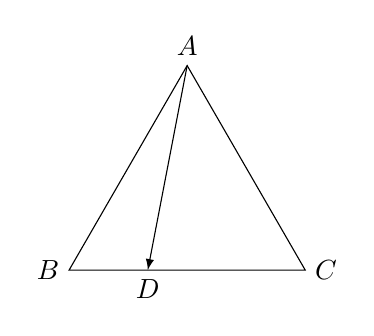
\begin{tikzpicture}[>=latex]
        \draw (0,0) node [left] {$B$} -- (3,0) node [right] {$C$} -- (1.5,{1.5*sqrt(3)}) node [above] {$A$} coordinate (A) -- cycle;
        \draw [->] (A) -- (1,0) node [below] {$D$};
    \end{tikzpicture}
\end{center}
\item {\tiny (000344)}定义在$\mathbf{R}$上的偶函数$y=f(x)$, 当$x\ge 0$时, $f(x)=\lg (x^2-3x+3)$, 则$f(x)$在$\mathbf{R}$上的零点个数为\blank{50}个.
\item {\tiny (000345)}将$6$辆不同的小汽车和$2$辆不同的卡车驶入如图所示的$10$个车位中的某$8$个内, 其中$2$辆卡车必须停在$A$与$B$的位置, 那么不同的停车位置安排共有\blank{50}种(结果用数值表示).
\begin{center}
    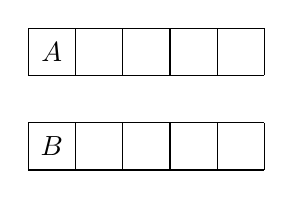
\begin{tikzpicture}[>=latex]
        \draw (0,0) node {$B$};
        \draw (0,1.2) node {$A$};
        \foreach \i in {-0.3,0.3,0.9,1.5}{\draw (-0.3,\i) -- (2.7,\i);};
        \foreach \i in {-0.3,0.3,...,2.8}{\draw (\i,-0.3) -- (\i, 0.3) (\i, 0.9) -- (\i, 1.5);};
    \end{tikzpicture}
\end{center}
\item {\tiny (000346)}设集合$A=\{x||x-2|<1,x\in \mathbf{R}\}$, 集合$B=\mathbf{Z}$, 则$A\cap B=$\blank{50}.
\item {\tiny (000347)}函数$y=\sin (\omega x-\dfrac{\pi}{3})$($\omega >0$)的最小正周期是$\pi$, 则$\omega =$\blank{50}.
\item {\tiny (000348)}设$\mathrm{i}$为虚数单位, 在复平面上, 复数$\dfrac{3}{(2-\mathrm{i})^2}$对应的点到原点的距离为\blank{50}.
\item {\tiny (000349)}若函数$f(x)=\log_2 (x+1)+a$的反函数的图像经过点$(4,1)$, 则实数$a=$\blank{50}.
\item {\tiny (000350)}已知$(a+3b)^n$的展开式中, 各项系数的和与各项二项式系数的和之比为$64$, 则$n=$\blank{50}.
\item {\tiny (000351)}甲、乙两人从$5$门不同的选修课中各选修$2$门, 则甲、乙所选的课程中恰有$1$门相同的选法有\blank{50}种.
\item {\tiny (000352)}若圆锥的侧面展开图是半径为2$\text{cm}$, 圆心角为$270^\circ$的扇形, 则这个圆锥的体积为\blank{50}$\text{cm}^3$.
\item {\tiny (000353)}若数列$\{a_n\}$的所有项都是正数, 且$\sqrt{a_1}+\sqrt{a_2}+\cdots +\sqrt{a_n}=n^2+3n$($n\in \mathbf{N}^*$), 则$\displaystyle\lim_{n\to\infty}\dfrac{1}{n^2}(\dfrac{a_1}{2}+\dfrac{a_2}{3}+\cdots +\dfrac{a_n}{n+1})=$\blank{50}.
\item {\tiny (000354)}如图, 在$\triangle ABC$中, $\angle B=45^\circ$, $D$是$BC$边上的一点, $AD=5$, $AC=7$, $DC=3$, 则$AB$的长为\blank{50}.
\begin{center}
    \begin{tikzpicture}[scale = 0.5]
        \draw  (-6.830127018922193,0.)-- (3.,0.) node [below right] {$C$};
        \draw  (3.,0.)-- (-2.5,4.330127018922193) node [above] {$A$};
        \draw  (-2.5,4.330127018922193)-- (-6.830127018922193,0.) node [below left] {$B$};
        \draw  (-2.5,4.330127018922193)-- (0.,0.) node [below] {$D$};
    \end{tikzpicture}
\end{center}
\item {\tiny (000355)}有以下命题:\\
\textcircled{1} 若函数$f(x)$既是奇函数又是偶函数, 则$f(x)$的值域为$\{0\}$; \\
\textcircled{2} 若函数$f(x)$是偶函数, 则$f(|x|)=f(x)$;\\
\textcircled{3} 若函数$f(x)$在其定义域内不是单调函数, 则$f(x)$不存在反函数;\\
\textcircled{4} 若函数$f(x)$存在反函数${{f}^{-1}}(x)$, 且${{f}^{-1}}(x)$与$f(x)$不完全相同, 则$f(x)$与${{f}^{-1}}(x)$图像的公共点必在直线$y=x$上; \\
其中真命题的序号是\blank{50}(写出所有真命题的序号).
\item {\tiny (000356)}若集合$A=\{x|y^2=x,y\in \mathbf{R}\}$, $B=\{y|y=\sin x,x\in \mathbf{R}\}$, 则$A\cap B=$\blank{50}.
\item {\tiny (000357)}若$-\dfrac{\pi}{2}<\alpha <\dfrac{\pi}{2}$, $\sin \alpha =\dfrac{3}{5}$, 则$\cot 2\alpha =$\blank{50}.
\item {\tiny (000358)}函数$f(x)=1+\log_2 x$($x\ge 1$)的反函数$f^{-1}(x)=$\blank{50}.
\item {\tiny (000359)}若$(1+x)^5=a_0+a_1x+a_2x^2+\cdots+a_5x^5$, 则$a_1+a_2+\cdots+a_5=$\blank{50}.
\item {\tiny (000360)}设$k\in \mathbf{R}$, $\dfrac{y^2}{k}-\dfrac{x^2}{k-2}=1$表示焦点在$y$轴上的双曲线, 则半焦距的取值范围是\blank{50}.
\item {\tiny (000361)}设$m\in \mathbf{R}$, 若$f(x)=(m+1)x^{\tfrac{2}{3}}+mx+1$是偶函数, 则$f(x)$的单调递增区间是\blank{50}.
\item {\tiny (000362)}方程$\log_2(9^x-5)=2+\log_2(3^x-2)$的解$x=$\blank{50}.
\item {\tiny (000363)}已知圆$C:x^2+y^2+2kx+2y+k^2=0$($k\in \mathbf{R}$)和定点$P(1,-1)$, 若过$P$可以作两条直线与圆$C$相切, 则$k$的取值范围是\blank{50}.
\item {\tiny (000364)}如图, 在直三棱柱$ABC-A_1B_1C_1$中, $\angle ABC=90^\circ$, $AB=BC=1$, 若$A_1C$与平面$B_1BCC_1$所成的角为$\dfrac{\pi}{6}$, 则三棱锥$A_1-ABC$的体积为\blank{50}.
\begin{center}
    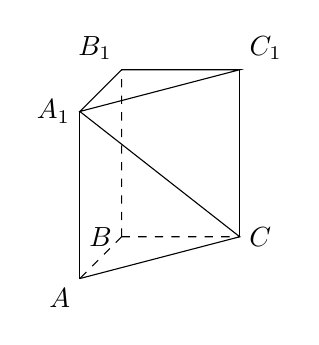
\begin{tikzpicture}[scale = 1.5]
        \draw [dashed] (0,0) -- (1,0) node [right] {$C$} coordinate (C) (0,0) -- (225:0.5) node [below left] {$A$} coordinate (A) (0,0) node [left] {$B$} coordinate (B) -- (0,{sqrt(2)}) node [above left] {$B_1$} coordinate (B1);
        \draw (A) --+ (0,{sqrt(2)}) node [left] {$A_1$} coordinate (A1);
        \draw (C) --+ (0,{sqrt(2)}) node [above right] {$C_1$} coordinate (C1);
        \draw (A1) -- (B1) -- (C1) -- (A1) -- (C) -- (A);
    \end{tikzpicture}
\end{center}
\item {\tiny (000365)}设地球半径为$R$, 若$A$、$B$两地均位于北纬$45^\circ$, 且两地所在纬度圈上的弧长为$\dfrac{\sqrt{2}}{4}\pi R$, 则$A$、$B$之间的球面距离是\blank{50}(结果用含有$R$的代数式表示).
\item {\tiny (000366)}复数$\mathrm{i}(2+\mathrm{i})$的虚部为\blank{50}.
\item {\tiny (000367)}设函数$f(x)=\begin{cases}\log_2 x, & x>0, \\ 4^x, & x\le 0,\end{cases}$ 则$f(f(-1))=$\blank{50}.
\item {\tiny (000368)}已知$M=\{x||x-1|\le 2,x\in \mathbf{R}\}$, $P=\{x|\dfrac{1-x}{x+2}\ge 0,x\in \mathbf{R}\}$, 则$M\cap P=$\blank{50}.
\item {\tiny (000369)}抛物线$y=x^2$上一点$M$到焦点的距离为$1$, 则点$M$的纵坐标为\blank{50}.
\item {\tiny (000370)}已知无穷数列$\{a_n\}$满足$a_{n+1}=\dfrac12{a_n}$($n\in \mathbf{N}^*$), 且$a_2=1$, 记$S_n$为数列$\{a_n\}$的前$n$项和, 则$\displaystyle\lim_{n\to \infty}S_n=$\blank{50}.
\item {\tiny (000371)}已知$x,y\in \mathbf{R}^+$, 且$x+2y=1$, 则$xy$的最大值为\blank{50}.
\item {\tiny (000372)}已知圆锥的母线$l=10$, 母线与旋转轴的夹角$\alpha =30^\circ$, 则圆锥的表面积为\blank{50}.
\item {\tiny (000373)}若$(2x^2+\dfrac1x)^n$($n\in \mathbf{N}^*$)的二项展开式中的第$9$项是常数项, 则$n=$\blank{50}.
\item {\tiny (000374)}已知$A,B$分别是函数$f(x)=2\sin \omega x$($\omega >0$)在$y$轴右侧图像上的第一个最高点和第一个最低点, 且$\angle AOB=\dfrac\pi 2$, 则该函数的最小正周期是\blank{50}.
\item {\tiny (000375)}将序号分别为1、2、3、4、5的$5$张参观券全部分给$4$人, 每人至少一张, 如果分给同一人的$2$张参观券连号, 那么不同的分法种数是\blank{50}.
\item {\tiny (000376)}$\displaystyle\lim_{n\to\infty}\dfrac{2n+3}{n+1}=$\blank{50}.
\item {\tiny (000377)}设全集$U=\mathbf{R}$, 集合$A=\{-1,0,1,2,3\}$, $B=\{x|x\ge 2\}$, 则$A\cap {\complement_U}B=$\blank{50}.
\item {\tiny (000378)}不等式$\dfrac{x+1}{x+2}<0$的解集为\blank{50}.
\item {\tiny (000379)}椭圆$\begin{cases} x=5\cos \theta,  \\ y=4\sin \theta  \end{cases}$($\theta$为参数)的焦距为\blank{50}.
\item {\tiny (000380)}若函数$y=\begin{vmatrix}   \cos x & \sin x  \\   \sin x & \cos x  \\ \end{vmatrix}$的最小正周期为$a\pi $, 则实数$a$的值为\blank{50}.
\item {\tiny (000381)}若点$(8,4)$在函数$f(x)=1+\log_a x$图像上, 则$f(x)$的反函数为\blank{50}.
\item {\tiny (000382)}已知向量$\overrightarrow{a}=(1,2)$, $\overrightarrow{b}=(0,3)$, 则$\overrightarrow{b}$在$\overrightarrow{a}$的方向上的投影为\blank{50}.
\item {\tiny (000383)}已知一个底面置于水平面上的圆锥, 其左视图是边长为6的正三角形, 则该圆锥的侧面积为\blank{50}.
\item {\tiny (000384)}某班级要从$5$名男生和$2$名女生中选出$3$人参加公益活动, 则在选出的$3$人中男、女生
均有的概率为\blank{50}(结果用最简分数表示).
\item {\tiny (000385)}设常数$a>0$, 若$(x+\dfrac ax)^9$的二项展开式中$x^5$的系数为$144$, 则$a=$\blank{50}.
\item {\tiny (000386)}设集合$M=\{x|x^2=x\}$, $N=\{x|\lg x\le 0\}$, 则$M\cap N=$\blank{50}.
\item {\tiny (000387)}已知$a$、$b\in \mathbf{R}$, $\mathrm{i}$是虚数单位, 若$a+\mathrm{i}=2-b\mathrm{i}$, 则$(a+b\mathrm{i})^2=$\blank{50}.
\item {\tiny (000388)}已知函数$f(x)=a^x-1$的图像经过$(1,1)$点, 则$f^{-1}(3)=$\blank{50}.
\item {\tiny (000389)}不等式$x|x-1|>0$的解集为\blank{50}.
\item {\tiny (000390)}已知$\overrightarrow a=(\sin x,\cos x)$, $\overrightarrow b=(\sin x,\sin x)$, 则函数$f(x)=\overrightarrow a\cdot \overrightarrow b$的最小正周期为\blank{50}.
\item {\tiny (000391)}里约奥运会游泳小组赛采用抽签方法决定运动员比赛的泳道, 在由$2$名中国运动员和$6$名外国运动员组成的小组中, $2$名中国运动员恰好抽在相邻泳道的概率为\blank{50}.
\item {\tiny (000392)}如图, 在棱长为$1$的正方体$ABCD-A_1B_1C_1D_1$中, 点$P$在截面$A_1DB$上, 则线段$AP$的最小值为\blank{50}.
\begin{center}
    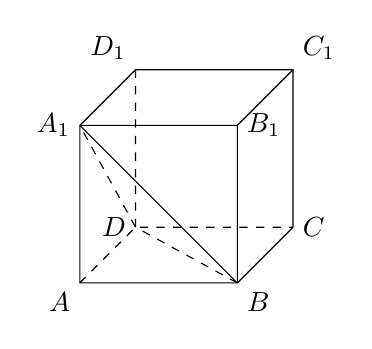
\begin{tikzpicture}
        \draw (0,0) node [below left] {$A$} coordinate (A) --++ (2,0) node [below right] {$B$} coordinate (B) --++ (45:{2/2}) node [right] {$C$} coordinate (C)
        --++ (0,2) node [above right] {$C_1$} coordinate (C1)
        --++ (-2,0) node [above left] {$D_1$} coordinate (D1) --++ (225:{2/2}) node [left] {$A_1$} coordinate (A1) -- cycle;
        \draw (A) ++ (2,2) node [right] {$B_1$} coordinate (B1) -- (B) (B1) --++ (45:{2/2}) (B1) --++ (-2,0);
        \draw [dashed] (A) --++ (45:{2/2}) node [left] {$D$} coordinate (D) --++ (2,0) (D) --++ (0,2);
        \draw (A1) -- (B);
        \draw [dashed] (B) -- (D) -- (A1);
    \end{tikzpicture}
\end{center}
\item {\tiny (000393)}设$(1+x)^n=a_0+a_1x+a_2x^2+a_3x^3+\cdots +a_nx^n$, 若$\dfrac{a_2}{a_3}=\dfrac13$, 则$n=$\blank{50}.
\item {\tiny (000394)}已知圆锥底面半径与球的半径都是$1\text{cm}$, 如果圆锥的体积与球的体积恰好也相等, 那么这个圆锥的侧面积是\blank{50}$\text{cm}^2$.
\item {\tiny (000395)}设$P(x,y)$是曲线$C:\sqrt{\dfrac{x^2}{25}}+\sqrt{\dfrac{y^2}9}=1$上的点, $F_1(-4,0)$, $F_2(4,0)$, 则$|PF_1|+|PF_2|$的最大值为\blank{50}.
\item {\tiny (000396)}已知复数$z=2+\mathrm{i}$($\mathrm{i}$为虚数单位), 则$\overline{{z^2}}=$\blank{50}.
\item {\tiny (000397)}已知集合$A=\{x|\dfrac12\le {2^x}<16\}$, $B=\{x|y=\log _2(9-x^2)\}$, 则$A\cap B=$\blank{50}.
\item {\tiny (000398)}在二项式$(x+\dfrac2x)^6$的展开式中, 常数项是\blank{50}.
\item {\tiny (000399)}等轴双曲线$x^2-y^2=a^2$与抛物线$y^2=16x$的准线交于$A$、$B$两点, 且$|AB|=4\sqrt3$, 则该双曲线的实轴长等于\blank{50}.
\item {\tiny (000400)}若由矩阵$\begin{pmatrix}a & 2 \\ 2 & a\end{pmatrix}\begin{pmatrix}x \\ y\end{pmatrix}=\begin{pmatrix}a+2 \\ 2a\end{pmatrix}$表示$x$、$y$的二元一次方程组无解, 则实数$a=$\blank{50}.
\item {\tiny (000401)}已知$f(x)=\sin\dfrac\pi 3x$, $A=\{1,2,3,4,5,6,7,8\}$, 现从集合$A$中任取两个不同元素$s$、$t$, 则使得$f(s)\cdot f(t)=0$发生的概率是\blank{50}.
\item {\tiny (000402)}若圆锥侧面积为$20\pi$, 且母线与底面所成角为$\arccos \dfrac45$, 则该圆锥的体积为\blank{50}.
\item {\tiny (000403)}已知数列$\{a_n\}$的通项公式为$a_n=n^2+bn$, 若数列$\{a_n\}$是单调递增数列, 则实数$b$的取值范围是\blank{50}.
\item {\tiny (000404)}将边长为$10$的正三角形$ABC$, 按``斜二测''画法在水平放置的平面上画出为$\triangle A'B'C'$, 则$\triangle A'B'C'$中最短边的边长为\blank{50}(精确到0.01).
\item {\tiny (000405)}已知点$A$是圆$O: x^2+y^2=4$上的一个定点, 点$B$是圆$O$上的一个动点, 若满足$|\overrightarrow{AO}+\overrightarrow{BO}|=|\overrightarrow{AO}-\overrightarrow{BO}|$, 则$\overrightarrow{AO}\cdot \overrightarrow{AB}=$\blank{50}.
\item {\tiny (000406)}方程$\lg (3x+4)=1$的解$x=$\blank{50}.
\item {\tiny (000407)}若关于$x$的不等式$\dfrac{x-a}{x-b}>0$($a,b\in \mathbf{R}$)的解集为$(-\infty ,1)\cup (4,+\infty)$, 则$a+b=$\blank{50}.
\item {\tiny (000408)}已知数列$\{a_n\}$的前$n$项和为$S_n=2^n-1$, 则此数列的通项公式为\blank{50}.
\item {\tiny (000409)}函数$f(x)=\sqrt x+1$的反函数是\blank{50}.
\item {\tiny (000410)}$(1+2x)^6$展开式中$x^3$项的系数为\blank{50}(用数字作答).
\item {\tiny (000411)}如图, 已知正方形$ABCD-A_1B_1C_1D_1$, $AA_1=2$, $E$为棱$CC_1$的中点, 则三棱锥$D_1-ADE$的体积为\blank{50}.
\begin{center}
    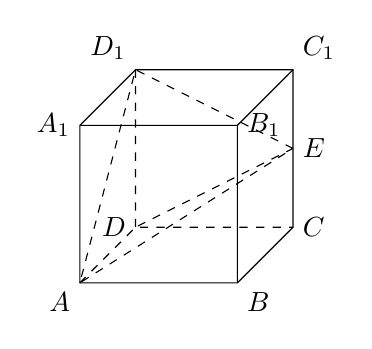
\begin{tikzpicture}
        \draw (0,0) node [below left] {$A$} coordinate (A) --++ (2,0) node [below right] {$B$} coordinate (B) --++ (45:{2/2}) node [right] {$C$} coordinate (C)
        --++ (0,2) node [above right] {$C_1$} coordinate (C1)
        --++ (-2,0) node [above left] {$D_1$} coordinate (D1) --++ (225:{2/2}) node [left] {$A_1$} coordinate (A1) -- cycle;
        \draw (A) ++ (2,2) node [right] {$B_1$} coordinate (B1) -- (B) (B1) --++ (45:{2/2}) (B1) --++ (-2,0);
        \draw [dashed] (A) --++ (45:{2/2}) node [left] {$D$} coordinate (D) --++ (2,0) (D) --++ (0,2);
        \draw ($ (C)!0.5!(C1) $) node [right] {$E$} coordinate (E);
        \draw [dashed] (E) -- (D1) -- (A) -- (E) -- (D);
    \end{tikzpicture}
\end{center}
\item {\tiny (000412)}从单词``shadow''中任意选取$4$个不同的字母排成一排, 则其中含有``a''的共有\blank{50}种排法(用数字作答).
\item {\tiny (000413)}集合$\{x|\cos (\pi \cos x)=0,x\in [0,\pi]\}=$\blank{50}(用列举法表示).
\item {\tiny (000414)}如图, 已知半径为1的扇形$AOB$, $\angle AOB=60^\circ$, $P$为弧$\overset\frown{AB}$上的一个动点, 则$\overrightarrow{OP}\cdot \overrightarrow{AB}$取值范围是\blank{50}.
\begin{center}
    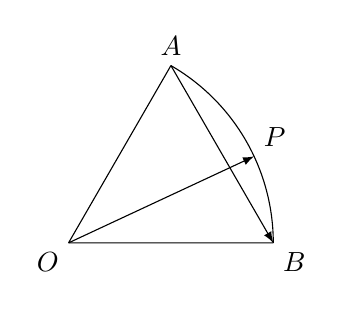
\begin{tikzpicture}[>=latex,scale = 1.3]
        \draw (0,0) node [below left] {$O$} -- (2,0) node [below right] {$B$} (0,0) -- (1,{sqrt(3)}) node [above] {$A$} -- cycle;
        \draw (2,0) arc (0:60:2);
        \draw [->] (0,0) -- (25:2) node [above right] {$P$};
        \draw [->] (1,{sqrt(3)}) -- (2,0);
    \end{tikzpicture}
\end{center}
\item {\tiny (000415)}已知$x$、$y$满足曲线方程$x^2+\dfrac1{y^2}=2$, 则$x^2+y^2$的取值范围是\blank{50}.
\item {\tiny (000416)}已知$U=\mathbf{R}$, 集合$A=\{x|4-2x\ge x+1\}$, 则${\complement_U}A=$\blank{50}.
\item {\tiny (000417)}三阶行列式$\begin{vmatrix}   3 & -5 & 1 \\   2 & 3 & -6 \\   -7 & 2 & 4 \\ \end{vmatrix}$中元素$-5$的代数余子式的值为\blank{50}.
\item {\tiny (000418)}$(1-\dfrac x2)^8$的二项展开式中含$x^2$项的系数是\blank{50}.
\item {\tiny (000419)}已知一个球的表面积为$16\pi$, 则它的体积为\blank{50}.
\item {\tiny (000420)}一个袋子中共有$6$个球, 其中$4$个红色球, $2$个蓝色球, 这些球的质地和形状一样, 从中任意抽取$2$个球, 则所抽的球都是红色球的概率是\blank{50}.
\item {\tiny (000421)}已知直线$l:x-y+b=0$被圆$C:x^2+y^2=25$所截得的弦长为$6$, 则$b=$\blank{50}.
\item {\tiny (000422)}若复数$(1+a\mathrm{i})(2-\mathrm{i})$在复平面上所对应的点在直线$y=x$上, 则实数$a=$\blank{50}.
\item {\tiny (000423)}函数$f(x)=(\sqrt3\sin x+\cos x)(\sqrt3\cos x-\sin x)$的最小正周期为\blank{50}.
\item {\tiny (000424)}过双曲线$C:\dfrac{x^2}{a^2}-\dfrac{y^2}4=1$的右焦点$F$作一条垂直于$x$轴的垂线交双曲线$C$的两条渐近线于$A$、$B$两点, $O$为坐标原点, 则$\triangle OAB$的面积的最小值为\blank{50}.
\item {\tiny (000425)}若关于$x$的不等式$|2^x-m|-\dfrac1{2^x}<0$在区间$[0,1]$内恒成立, 则实数$m$的范围\blank{50}.
\item {\tiny (000426)}已知集合$A=\{1,2,4,6,8\}$, $B=\{x|x=2k,k\in A\}$, 则$A\cap B=$\blank{50}.
\item {\tiny (000427)}已知$\dfrac{\overline z}{1-\mathrm{i}}=2+\mathrm{i}$, 则复数$z$的虚部为\blank{50}.
\item {\tiny (000428)}设函数$f(x)=\sin x-\cos x$, 且$f(a)=1$, 则$\sin 2a=$\blank{50}.
\item {\tiny (000429)}已知二元一次方程$\begin{cases} {a_1}x+{b_1}y={c_1}, \\  {a_2}x+{b_2}y={c_2} \end{cases}$的增广矩阵是$\begin{pmatrix} 1 & -1 & 1 \\  1 & 1 & 3 \\ \end{pmatrix}$, 则此方程组的解是\blank{50}.
\item {\tiny (000430)}数列$\{a_n\}$是首项为$1$, 公差为$2$的等差数列, $S_n$是它前$n$项和, 则$\displaystyle\lim_{n\to\infty}\dfrac{S_n}{a_n^2}=$\blank{50}.
\item {\tiny (000431)}已知角$A$是$\triangle ABC$的内角, 则``$\cos A=\dfrac12$''是``$\sin A=\dfrac{\sqrt3}2$''的\blank{50}条件(填``充分非必要''、``必要非充分''、``充要条件''、``既非充分又非必要''之一).
\item {\tiny (000432)}若双曲线$x^2-\dfrac{y^2}{b^2}=1$的一个焦点到其渐近线距离为$2\sqrt2$, 则该双曲线焦距等于\blank{50}.
\item {\tiny (000433)}若正项等比数列$\{a_n\}$满足: $a_3+a_5=4$, 则$a_4$的最大值为\blank{50}.
\item {\tiny (000434)}已知函数$f(x)=\sin (2x+\dfrac\pi 3)$在区间$[0,a]$(其中$a>0$)上单调递增, 则实数$a$的取值范围是\blank{50}.
\item {\tiny (000435)}设函数$f(x)=\begin{cases}    x^6, & x\ge 1,  \\   -2x-1, & x\le -1, \end{cases}$ 则当$x\le -1$时, $f[f(x)]$表达式的展开式中含${x^2}$项的系数是\blank{50}.
\item {\tiny (000436)}``$x<0$''是``$x<a$''的充分非必要条件, 则$a$的取值范围是\blank{50}.
\item {\tiny (000437)}函数$f(x)=1-3\sin ^2(x+\dfrac\pi 4)$的最小正周期为\blank{50}.
\item {\tiny (000438)}若复数$z$为纯虚数, 且满足$(2-\mathrm{i})z=a+\mathrm{i}$($\mathrm{i}$为虚数单位), 则实数$a$的值为\blank{50}.
\item {\tiny (000439)}二项式$(x^2+\dfrac 1x)^5$的展开式中, $x$的系数为\blank{50}.
\item {\tiny (000440)}用半径$1$米的半圆形薄铁皮制作圆锥型无盖容器, 其容积为\blank{50}立方米.
\item {\tiny (000441)}已知$\alpha$为锐角, 且$\cos (\alpha +\dfrac\pi 4)=\dfrac35$, 则$\sin \alpha =$\blank{50}.
\item {\tiny (000442)}已知正四棱柱$ABCD-A_1B_1C_1D_1$, $AB=a$, $AA_1=2a$, $E$、$F$分别是棱$AD$、$CD$的中点,则异面直线$BC_1$与$EF$所成角是\blank{50}.
\item {\tiny (000443)}在无穷等比数列$\{a_n\}$中, $\displaystyle\lim_{n\to\infty}(a_1+a_2+\cdots+a_n)=\dfrac12$, 则$a_1$的取值范围是\blank{50}.
\item {\tiny (000444)}某班班会准备从含甲、乙的$6$名学生中选取$4$人发言, 要求甲、乙两人至少有一人参加, 那么不同的发言顺序有\blank{50}种.
\item {\tiny (000445)}已知奇函数$f(x)$是定义在$\mathbf{R}$上的增函数, 数列$\{x_n\}$是一个公差为$2$的等差数列, 满足$f(x_7)+f(x_8)=0$, 则$x_{2017}$的值为\blank{50}.
\item {\tiny (000446)}若集合$M=\{x|{x^2}-2x<0\}$, $N=\{x||x|>1\}$, 则$M\cap N=$\blank{50}.
\item {\tiny (000447)}若复数$\angle OFA+\angle OFB={180^\circ}$满足$2z+\overline z=3-2\mathrm{i}$, 其中$\mathrm{i}$为虚数单位, 则$z=$\blank{50}.
\item {\tiny (000448)}如果$\sin \alpha =-\dfrac5{13}$, 且$\alpha$为第四象限角, 则$\tan \alpha$的值是\blank{50}.
\item {\tiny (000449)}函数$f(x)=\begin{vmatrix}   \cos x & \sin x  \\    \sin x & \cos x \end{vmatrix}$的最小正周期是\blank{50}.
\item {\tiny (000450)}函数$f(x)=2^x+m$的反函数为$y=f^{-1}(x)$, 且$y=f^{-1}(x)$的图像过点$Q(5,2)$, 那么$m=$\blank{50}.
\item {\tiny (000451)}点$(1,0)$到双曲线$\dfrac{x^2}4-y^2=1$的渐近线的距离是\blank{50}.
\item {\tiny (000452)}如果实数$x$、$y$满足$\begin{cases} 2x-y\le 0, \\ x+y\le 3, \\  x\ge 0, \\ \end{cases}$, 则$2x+y$的最大值是\blank{50}.
\item {\tiny (000453)}从$5$名学生中任选$3$人分别担任语文、数学、英语课代表, 其中学生甲不能担任数学课代表, 共有\blank{50}种不同的选法(结果用数值表示).
\item {\tiny (000454)}方程$x^2+y^2-4tx-2ty+3t^2-4=0$($t$为参数)所表示的圆的圆心轨迹方程是\blank{50}(结果化为普通方程).
\item {\tiny (000455)}若$a_n$是$(2+x)^n$($n\in \mathbf{N}^*$, $n\ge 2$, $x\in \mathbf{R}$)展开式中$x^2$项的二项式系数, 则$\displaystyle\lim_{n\to\infty}(\dfrac 1{a_2}+\dfrac 1{a_3}+\cdots+\dfrac1{a_n})=$\blank{50}.
\item {\tiny (000456)}设集合$A=\{2,3,4,12\}$, $B=\{0,1,2,3\}$, 则$A\cap B=$\blank{50}.
\item {\tiny (000457)}$\displaystyle\lim_{n\to\infty}\dfrac{5^n-7^n}{5^n+7^n}=$\blank{50}.
\item {\tiny (000458)}函数$y=2\cos^2(3\pi x)-1$的最小正周期为\blank{50}.
\item {\tiny (000459)}不等式$\dfrac{x+2}{x+1}>1$的解集为\blank{50}.
\item {\tiny (000460)}若$z=\dfrac{-2+3\mathrm{i}}{\mathrm{i}}$(其中$\mathrm{i}$为虚数单位), 则$\mathrm{Im} z=$\blank{50}.
\item {\tiny (000461)}若从五个数$-1,0,1,2,3$中任选一个数$m$, 则使得函数$f(x)=(m^2-1)x+1$在$\mathbf{R}$上单调递增的概率为\blank{50}(结果用最简分数表示).
\item {\tiny (000462)}在$(\dfrac3{x^2}+\sqrt{x})^n$的二项展开式中, 所有项的二项式系数之和为$1024$, 则常数项的值等于\blank{50}.
\item {\tiny (000463)}半径为$4$的圆内接三角形$ABC$的面积是$\dfrac1{16}$, 角$A,B,C$所对应的边依次为$a,b,c$, 则$abc$的值为\blank{50}.
\item {\tiny (000464)}已知抛物线$C$的顶点为坐标原点, 双曲线$\dfrac{x^2}{25}-\dfrac{y^2}{144}=1$的右焦点是$C$的焦点$F$. 若斜率为$-1$, 且过$F$的直线与$C$交于$A,B$两点, 则$|AB|=$\blank{50}.
\item {\tiny (000465)}直角坐标系$xOy$内有点$P(-2,-1)$, $Q(0,-2)$, 将$\triangle POQ$绕$x$轴旋转一周, 则所得几何体的体积为\blank{50}.
\item {\tiny (000466)}已知集合$A=\{1,2,5\}$, $B=\{2,a\}$. 若$A\cup B=\{1,2,3,5\}$, 则$a=$\blank{50}.
\item {\tiny (000467)}抛物线$y^2=4x$的焦点坐标是\blank{50}.
\item {\tiny (000468)}不等式$\dfrac x{x+1}<0$的解是\blank{50}.
\item {\tiny (000469)}若复数$z$满足$\mathrm{i}z=1+\mathrm{i}$($\mathrm{i}$为虚数单位), 则$z=$\blank{50}.
\item {\tiny (000470)}在代数式$(x+\dfrac 1{x^2})^7$的展开式中, 一次项的系数是\blank{50}(用数字作答).
\item {\tiny (000471)}若函数$y=2\sin (\omega x-\dfrac\pi 3)+1 \ (\omega >0)$的最小正周期是$\pi$, 则$\omega=$\blank{50}.
\item {\tiny (000472)}若函数$f(x)=x^a$的反函数的图像经过点$(\dfrac12,\dfrac14)$, 则$a=$\blank{50}.
\item {\tiny (000473)}将一个正方形绕着它的一边所在的直线旋转一周, 所得几何体的体积为$27\pi\text{cm}^3$, 则该几何体的侧面积为\blank{50}$\text{cm}^3$.
\item {\tiny (000474)}已知函数$y=f(x)$是奇函数, 当$x<0$时, $f(x)=2^x-ax$, 且$f(2)=2$, 则$a=$\blank{50}.
\item {\tiny (000475)}若无穷等比数列$\{a_n\}$的各项和为$S_n$, 首项$a_1=1$, 公比为$a-\dfrac32$, 且$\displaystyle\lim_{n\to\infty}S_n=a$, 则$a=$\blank{50}.
\item {\tiny (000476)}已知全集$U=\mathbf{N}$, 集合$A=\{1,2,3,4\}$, 集合$B=\{3,4,5\}$, 则$(\complement_U A)\cap B=$\blank{50}.
\item {\tiny (000477)}复数$\dfrac2{1+\mathrm{i}}$的虚部是\blank{50}.
\item {\tiny (000478)}用$1,2,3,4,5$共$5$个数排成一个没有重复数字的三位数, 则这样的三位数有\blank{50}个.
\item {\tiny (000479)}已知$\tan \theta =-2$, 且$\theta \in (\dfrac\pi 2,\pi)$, 则$\cos\theta=$\blank{50}.
\item {\tiny (000480)}圆锥的底面半径为$1$, 母线长为$3$, 则圆锥的侧面积等于\blank{50}.
\item {\tiny (000481)}已知向量$\overrightarrow{a}=(1,\sqrt{3})$, $\overrightarrow{b}=(3,m)$. 若向量$\overrightarrow{b}$在$\overrightarrow{a}$方向上的投影为$3$, 则实数$m=$\blank{50}.
\item {\tiny (000482)}已知球主视图的面积等于$9\pi$, 则该球的体积为\blank{50}.
\item {\tiny (000483)}$(x+\dfrac{1}{x^2})^9$的二项展开式中, 常数项的值为\blank{50}.
\item {\tiny (000484)}已知$A(2,0)$, $B(4,0)$, 动点$P$满足$|PA|=\dfrac{\sqrt2} 2|PB|$, 则$P$到原点的距离为\blank{50}.
\item {\tiny (000485)}设焦点为$F_1$、$F_2$的椭圆$\dfrac{x^2}{a^2}+\dfrac{y^2}3=1 \ (a>0)$上的一点$P$也在抛物线$y^2=\dfrac94x$上, 抛物线焦点为$F_3$, 若$|PF_3|=\dfrac{25}{16}$, 则$\triangle PF_1F_2$的面积为\blank{50}.
\item {\tiny (000486)}函数$f(x)=\lg(2-x)$的定义域是\blank{50}.
\item {\tiny (000487)}已知$f(x)$是定义在$\mathbf{R}$上的奇函数, 则$f(-1)+f(0)+f(1)=$\blank{50}.
\item {\tiny (000488)}首项和公比均为$\dfrac12$的等比数列$\{a_n\}$, $S_n$是它的前$n$项和, 则$\displaystyle\lim_{n\to\infty}S_n=$\blank{50}.
\item {\tiny (000489)}在$\triangle ABC$中, $\angle A,\angle B,\angle C$所对的边分别是$a,b,c$, 若$a:b:c=2:3:4 $, 则$\cos C=$\blank{50}.
\item {\tiny (000490)}已知复数$z=a+b\mathrm{i}(a,b\in \mathbf{R})$满足$|z|=1$, 则$a\cdot b$范围是\blank{50}.
\item {\tiny (000491)}某学生要从物理、化学、生物、政治、历史、地理这六门学科中选三门参加等级考, 要求是物理、化学、生物这三门至少要选一门, 政治、历史、地理这三门也至少要选一门, 则该生的可能选法总数是\blank{50}.
\item {\tiny (000492)}已知$M$、$N$是三棱锥$P-ABC$的棱$AB$, $PC$的中点, 记三棱锥$P-ABC$的体积为$V_1$, 三棱锥$N-MBC$的体积为$V_2$, 则$\dfrac{V_2}{V_1}$等于\blank{50}.
\item {\tiny (000493)}在平面直角坐标系中, 双曲线$\dfrac{x^2}{a^2}-y^2=1 $的一个顶点与抛物线$y^2=12x$的焦点重合, 则双曲线的两条渐近线的方程为\blank{50}.
\item {\tiny (000494)}已知$y=\sin x$和$y=\cos x$的图像的连续的三个交点$A$、$B$、$C$构成三角形$\triangle ABC$, 则$\triangle ABC$的面积等于\blank{50}.
\item {\tiny (000495)}已知函数$f(x)=\begin{cases} 2^x, & x\le 0, \\ f(x-2), & x>0, \end{cases}$ 则$f(1)+f(2)+f(3)+\cdots+f(2017)=$\blank{50}.
\item {\tiny (000496)}已知全集$U=\mathbf{R}$, 集合$A=\{x||x-1|>1\}$, $B=\{x|\dfrac{x-3}{x+1}<0\}$, 则$(\complement_U A)\cap B=$\blank{50}.
\item {\tiny (000497)}已知角$\theta$的顶点在坐标原点, 始边与$x$轴的正半轴重合, 若角$\theta$的终边落在第三象限内, 且$\cos(\dfrac\pi 2+\theta)=\dfrac35$, 则$\cos 2\theta=$\blank{50}.
\item {\tiny (000498)}已知幂函数的图像过点$(2,\dfrac14)$, 则该幂函数的单调递增区间是\blank{50}.
\item {\tiny (000499)}若$S_n$是等差数列$\{a_n\}\ (n\in \mathbf{N}^*)$: $-1,2,5,8,\cdots$的前$n$项和, 则$\displaystyle\lim_{n\to\infty}\dfrac{{S_n}}{{n^2}+1}=$\blank{50}.
\item {\tiny (000500)}某圆锥体的底面圆的半径长为$\sqrt2$, 其侧面展开图是圆心角为$\dfrac23\pi$的扇形, 则该圆锥体的体积是\blank{50}.
\item {\tiny (000501)}过点$P(-2,1)$作圆$x^2+y^2=5$的切线, 则该切线的点法向式方程是\blank{50}.
\item {\tiny (000502)}已知二项式展开式$(1-2x)^7=a_0+a_1x+a_2x^2+\cdots +a_7x^7$, 且复数$z=\dfrac12a_1+\dfrac{a_7}{128}\mathrm{i}$, 则复数$z$的模$|z|=$\blank{50}(其中$\mathrm{i}$是虚数单位).
\item {\tiny (000503)}某高级中学欲从本校的$7$位古诗词爱好者(其中男生$2$人、女生$5$人)中随机选取$3$名同学作为学校诗词朗读比赛的主持人. 若要求主持人中至少有一位是男同学, 则不同选取方法的种数是\blank{50}(结果用数值表示).
\item {\tiny (000504)}已知$\triangle ABC$的三个内角$A,B,C$所对边长分别为$a,b,c$, 记$\triangle ABC$的面积为$S$, 若$S=a^2-(b-c)^2$, 则内角$A=$\blank{50}(结果用反三角函数值表示).
\item {\tiny (000505)}已知函数$f(x)=\left|\dfrac1{|x|-1}\right|$, 关于$x$的方程$f^2(x)+bf(x)+c=0$有$7$个不同实数根, 则实数$b,c$满足的关系式是\blank{50}.
\item {\tiny (000506)}若全集$U=\mathbf{R}$, 集合$A=\{x|x\le 0\text{或} x\ge 2\}$, 则$\complement_U A=$\blank{50}.
\item {\tiny (000507)}不等式$\dfrac{x-1}x<0$的解为\blank{50}.
\item {\tiny (000508)}方程组$\begin{cases} 3x-2y=1, \\ 2x+3y=5 \end{cases}$的增广矩阵是\blank{50}.
\item {\tiny (000509)}若复数$z=2-\mathrm{i}$($\mathrm{i}$为虚数单位), 则$z\cdot \overline z+z$=\blank{50}.
\item {\tiny (000510)}已知$F_1$、$F_2$是椭圆$\dfrac{x^2}{25}+\dfrac{y^2}9=1$的两个焦点, $P$是椭圆上的一个动点, 则$|PF1|\times |PF2|$的最大值是\blank{50}.
\item {\tiny (000511)}已知$x, y$满足$\begin{cases}x-y+1 \ge 0, \\ x+y-3 \ge 0, \\  x\le 2, \end{cases}$ 则目标函数$k=2x+y$的最大值为\blank{50}.
\item {\tiny (000512)}从一副混合后的扑克牌($52$张)中随机抽取$1$张, 事件$A$为``抽得红桃K'', 事件$B$为``抽得为黑桃'', 则概率$P(A\cup B)=$\blank{50}(结果用最简分数表示).
\item {\tiny (000513)}已知点$A(2,3)$、点$B(-2,\sqrt3)$, 直线$l$过点$P(-1,0)$, 若直线$l$与线段$AB$相交, 则直线$l$的倾斜角的取值范围是\blank{50}.
\item {\tiny (000514)}数列$\{a_n\}$的通项公式是$a_n=2n-1\ (n\in \mathbf{N}^*)$, 数列$\{b_n\}$的通项公式是$b_n=3n \ (n\in \mathbf{N}^*)$, 令集合$A=\{a_1,a_2,\cdots,a_n,\cdots\}$, $B=\{b_1,b_2,\cdots,b_n,\cdots\}$, $n\in \mathbf{N}^*$. 将集合$A\cup B$中的所有元素按从小到大的顺序排列, 构成的数列记为$\{c_n\}$. 则数列$\{c_n\}$的前$28$项的和$S_{28}=$\blank{50}.
\item {\tiny (000515)}向量$\overrightarrow{i}$、$\overrightarrow{j}$是平面直角坐标系$x$轴、$y$轴的基本单位向量, 且$|\overrightarrow a-\overrightarrow i|+|\overrightarrow a-2\overrightarrow j|=\sqrt5$, 则$|\overrightarrow a+2 \overrightarrow i|$的取值范围为\blank{50}.
\item {\tiny (000516)}计算: $\displaystyle\lim_{n\to\infty}(1-\dfrac n{n+1})=$\blank{50}.
\item {\tiny (000517)}计算行列式$\begin{vmatrix} 1-\mathrm{i} & 2 \\ 3\mathrm{i}+1 & 1+\mathrm{i}\end{vmatrix}$的结果是\blank{50}(其中$\mathrm{i}$为虚数单位).
\item {\tiny (000518)}与双曲线$\dfrac{x^2}9-\dfrac{y^2}{16}=1$的渐近线相同, 且经过点$A(-3,2 \sqrt3)$的双曲线的方程是\blank{50}.
\item {\tiny (000519)}从$5$名志愿者中选出$3$名, 分别从事布置、迎宾、策划三项不同的工作, 每人承担一项工作, 则不同的选派方案共有\blank{50}种(结果用数值表示).
\item {\tiny (000520)}已知函数$f(x)=a\cdot 2^x+3-a\ (a\in \mathbf{R})$的反函数为$y=f^{-1}(x)$, 则函数$y=f^{-1}(x)$的图像经过的定点的坐标为\blank{50}.
\item {\tiny (000521)}在$(x-a)^{10}$的展开式中, $x^7$的系数是$15$, 则实数$a=$\blank{50}.
\item {\tiny (000522)}已知点$A(2,3)$到直线$ax+(a-1)y+3=0$的距离不小于$3$, 则实数$a$的取值范围是\blank{50}.
\item {\tiny (000523)}类似平面直角坐标系, 我们把平面内两条相交但不垂直的数轴构成的坐标系(两条数轴的原点重合于$O$点且单位长度相同)称为斜坐标系. 在斜坐标系$xOy$中, 若$\overrightarrow{OP}=x\overrightarrow{e_1}+y\overrightarrow{e_2}$(其中$\overrightarrow{e_1},\overrightarrow{e_2}$分别为斜坐标系的$x$轴、$y$轴正方向上的单位向量, $x,y\in \mathbf{R}$), 则点$P$的坐标为$(x,y)$.若在斜坐标系$xOy$中, $\angle xOy=60^\circ$, 点$M$的坐标为$(1,2)$, 则点$M$到原点$O$的距离为\blank{50}.
\item {\tiny (000524)}已知圆锥的轴截面是等腰直角三角形, 该圆锥的体积为$\dfrac83\pi$, 则该圆锥的侧面积等于\blank{50}.
\item {\tiny (000525)}已知函数$f(x)=\begin{cases} (5-a)x+1, & x<1, \\ a^x, & x\ge 1\end{cases} \ (a>0,a\ne 1)$是实数集$\mathbf{R}$上的增函数, 则实数$a$的取值范围为\blank{50}.
\item {\tiny (000526)}集合$P=\{x|0 \le x<3, x\in \mathbf{Z}\}$, $M=\{x|x^2 \le 9\}$, 则$P\cap M=$\blank{50}.
\item {\tiny (000527)}计算$\displaystyle\lim_{n\to\infty}\dfrac{\mathrm{C}_n^2}{n^2+1}=$\blank{50}.
\item {\tiny (000528)}方程$\begin{vmatrix} 1+\lg x & 3-\lg x  \\   1 & 1  \end{vmatrix}=0$的根是\blank{50}.
\item {\tiny (000529)}已知$\sin \alpha -\dfrac35+(\cos \alpha -\dfrac45)\mathrm{i}$是纯虚数($\mathrm{i}$是虚数单位), 则$sin(\alpha +\dfrac{\pi}4)=$\blank{50}.
\item {\tiny (000530)}已知直线$l$的一个法向量是$\overrightarrow{n}=(\sqrt3,-1)$, 则$l$的倾斜角的大小是\blank{50}.
\item {\tiny (000531)}从$4$名男同学和$6$名女同学中选取$3$人参加某社团活动, 选出的$3$人中男女同学都有的不同选法种数是\blank{50}(用数字作答).
\item {\tiny (000532)}在$(1+2x)^5$的展开式中, $x^2$项系数为\blank{50}(用数字作答).
\item {\tiny (000533)}如图, 在直三棱柱$ABC-A_1B_1C_1$中, $\angle ACB=90^\circ$, $AC=4$, $BC=3$, $AB=BB_1$, 则异面直线$A_1B$与$B_1C_1$所成角的大小是\blank{50}(结果用反三角函数表示).
\begin{center}
    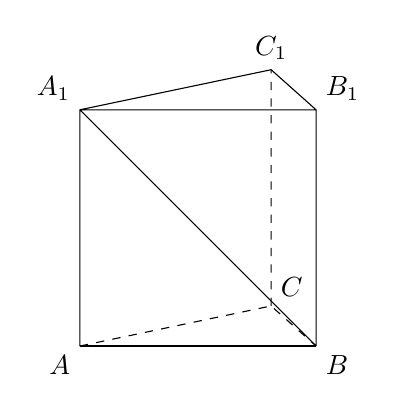
\begin{tikzpicture}[scale = 0.6]
        \draw (0,0) node [below left] {$A$} coordinate (A) -- (5,0) node [below right] {$B$} coordinate (B);
        \draw (3.2,0) + (45:1.2) node [above right] {$C$} coordinate (C);
        \draw [dashed] (A) -- (C) --(B);
        \draw (A) + (0,5) node [above left] {$A_1$} coordinate (A1);
        \draw (B) + (0,5) node [above right] {$B_1$} coordinate (B1);
        \draw (C) + (0,5) node [above] {$C_1$} coordinate (C1);
        \draw (A) -- (A1) -- (B1) -- (B) (A1) -- (C1) -- (B1) (A1) -- (B);
        \draw [dashed] (C) -- (C1);
    \end{tikzpicture}
\end{center}
\item {\tiny (000534)}已知数列$\{a_n\}$, $\{b_n\}$满足$b_n=\ln a_n$, $n\in \mathbf{N}^*$, 其中$\{b_n\}$是等差数列, 且$a_3\cdot a_{1007}=\mathrm{e}^4$, 则$b_1+b_2+\cdots +b_{1009}=$\blank{50}.
\item {\tiny (000535)}如图, 向量$\overrightarrow{OA}$与$\overrightarrow{OB}$的夹角为$120^\circ$, $|\overrightarrow{OA}|=2$, $|\overrightarrow{OB}|=1$, $P$是以$O$为圆心、$|\overrightarrow{OB}|$为半径的弧$\overset\frown{BC}$上的动点, 若$\overrightarrow{OP}=\lambda \overrightarrow{OA}+\mu \overrightarrow{OB}$, 则$\lambda \mu$的最大值是\blank{50}.
\begin{center}
    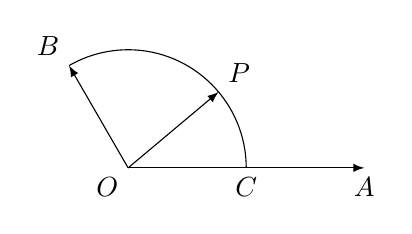
\begin{tikzpicture}[scale = 1.5, >=latex]
        \draw [->] (0,0) node [below left] {$O$} -- (2,0) node [below] {$A$};
        \draw [->] (0,0) --+ (120:1) node [above left] {$B$};
        \draw [->] (0,0) --+ (40:1) node [above right] {$P$};
        \draw (1,0) node [below] {$C$} arc (0:120:1);
    \end{tikzpicture}
\end{center}
\item {\tiny (000536)}设全集$U=\{ 1,2,3,4,5\}$, 若集合$A=\{3,4,5\}$, 则$\complement_U A=$\blank{50}.
\item {\tiny (000537)}若$\sin\theta=\dfrac14$, 则$\cos(\dfrac{3 \pi}2+\theta)=$\blank{50}.
\item {\tiny (000538)}方程$\log_2(2-x)+\log_2(3-x)=\log_2 12$的解$x=$\blank{50}.
\item {\tiny (000539)}$(\sqrt x-\dfrac1x)^9$的二项展开式中的常数项的值为\blank{50}.
\item {\tiny (000540)}不等式$\dfrac1{|x-1|}\ge 1 $的解集为\blank{50}.
\item {\tiny (000541)}函数$f(x)=\sqrt 3\sin x+2\cos^2\dfrac x2$的值域为\blank{50}.
\item {\tiny (000542)}已知$\mathrm{i}$是虚数单位, $\overline z$是复数$z$的共轭复数, 若$\begin{vmatrix} z & 1+\mathrm{i}  \\ 1 & 2\mathrm{i} \end{vmatrix}=0$, 则$\overline z$在复平面内所对应的点所在的象限为第\blank{50}象限.
\item {\tiny (000543)}若数列$\{a_n\}$的前$n$项和$S_n=-3n^2+2n+1 \ (n\in \mathbf{N}^*)$, 则$\displaystyle\lim_{n\to\infty}\dfrac{a_n}{3n}=$\blank{50}.
\item {\tiny (000544)}若直线$l:x+y=5$与曲线$C:x^2+y^2=16$交于两点$A(x_1,y_1)$, $B(x_2,y_2)$, 则$x_1y_2+x_2y_1$的值为\blank{50}.
\item {\tiny (000545)}设$a_1,a_2,a_3,a_4$是$1,2,3,4$的一个排列, 若至少有一个$i\ (i=1,2,3,4)$使得$a_i=i$成立, 则满足此条件的不同排列的个数为\blank{50}.
\item {\tiny (000546)}计算: $\displaystyle\lim_{n\to\infty}\dfrac{2n}{3n-1}=$\blank{50}.
\item {\tiny (000547)}已知集合$A=\{x|0<x<3\}$, $B=\{x|x^2\ge 4\}$, 则$A\cap B=$\blank{50}.
\item {\tiny (000548)}已知$\{a_n\}$为等差数列, $S_n$为其前$n$项和, 若$a_1+a_9=18$, $a_4=7 $, 则$S_{10}=$\blank{50}.
\item {\tiny (000549)}已知函数$f(x)=\log_2(x+a)$的反函数为$y=f^{-1}(x)$, 且$f^{-1}(2)=1$, 则实数$a=$\blank{50}.
\item {\tiny (000550)}已知角$\alpha$的终边与单位圆$x^2+y^2=1$交于点$P(\dfrac12,y_0)$, 则$\cos 2 \alpha$=\blank{50}.
\item {\tiny (000551)}若存在$x\in [0,+\infty)$使$\begin{vmatrix}2^x & 2^x \\ m & x \end{vmatrix}<1$成立, 则实数$m$的取值范围是\blank{50}.
\item {\tiny (000552)}函数$y=\sin 2x$的图像与$y=\cos x$的图像在区间$[0,2\pi]$上交点的个数是\blank{50}.
\item {\tiny (000553)}若直线$ax-y+3=0$与圆$(x-1)^2+(y-2)^2=4$相交于$A$、$B$两点, 且$|AB|=2 \sqrt3$, 则$a$=\blank{50}.
\item {\tiny (000554)}在$\triangle ABC$中, $\angle A=90^\circ $, $\triangle ABC$的面积为$1$. 若$\overrightarrow{BM}=\overrightarrow{MC}$, $\overrightarrow{BN}=4 \overrightarrow{NC}$, 则$\overrightarrow{AM}\cdot \overrightarrow{AN}$的最小值为\blank{50}.
\item {\tiny (000555)}已知函数$f(x)=x|2x-a|-1$有三个零点, 则实数$a$的取值范围为\blank{50}.
\item {\tiny (000556)}设全集$U=\mathbf{Z}$, 集合$M=\{1,2\}$, $P=\{-2,-1,0,1,2\}$, 则$P\cap \complement_U M$=\blank{50}.
\item {\tiny (000557)}已知复数$z=\dfrac{\mathrm{i}}{2+\mathrm{i}}$($\mathrm{i}$为虚数单位), 则$z\cdot \overline z$=\blank{50}.
\item {\tiny (000558)}不等式$2^{x^2-4x-3}>(\dfrac12 )^{3(x-1)}$的解集为\blank{50}.
\item {\tiny (000559)}函数$f(x)=\sqrt3\sin x\cos x+\cos^2x$的最大值为\blank{50}.
\item {\tiny (000560)}在平面直角坐标系$xOy$中, 以直线$y=\pm 2x$为渐近线, 且经过椭圆$x^2+\dfrac{y^2}4=1$右顶点的双曲线的方程是\blank{50}.
\item {\tiny (000561)}将圆锥的侧面展开后得到一个半径为$2$的半圆, 则此圆锥的体积为\blank{50}.
\item {\tiny (000562)}设等差数列$\{a_n\}$的公差$d$不为$0$, $a_1=9d$. 若$a_k$是$a_1$与$a_{2k}$的等比中项, 则$k=$\blank{50}.
\item {\tiny (000563)}已知$(1+2x)^6$展开式的二项式系数的最大值为$a$, 系数的最大值为$b$, 则$\dfrac ba=$\blank{50}.
\item {\tiny (000564)}同时掷两枚质地均匀的骰子, 则两个点数之积不小于$4$的概率为\blank{50}.
\item {\tiny (000565)}已知函数$f(x)=\begin{cases} \log_2 (x+a), & x\le 0, \\ x^2-3ax+a, & x>0 \end{cases}$有三个不同的零点, 则实数$a$的取值范围是\blank{50}.
\item {\tiny (000566)}在复平面内, 复数$\dfrac{5+4\mathrm{i}}{\mathrm{i}}$($\mathrm{i}$为虚数单位)对应的点的坐标为\blank{50}.
\item {\tiny (000567)}函数$f(x)=\sqrt{1-\lg x}$的定义域为\blank{50}.
\item {\tiny (000568)}二项式$(x-\dfrac1{2x})^4$的展开式中的常数项为\blank{50}.
\item {\tiny (000569)}若$\begin{vmatrix} 4^x & 2 \\ 2^x & 1 \end{vmatrix}=0$, 则$x=$\blank{50}.
\item {\tiny (000570)}已知圆$O:x^2+y^2=1$与圆$O'$关于直线$x+y=5$对称, 则圆$O'$的方程是\blank{50}.
\item {\tiny (000571)}在坐标平面$xOy$内, $O$为坐标原点, 已知点$A(-\dfrac12,\dfrac{\sqrt3}2)$, 将$\overrightarrow{OA}$绕原点按顺时针方向旋转$\dfrac{\pi}2$, 得到$\overrightarrow{OA'}$, 则$\overrightarrow{OA'}$的坐标为\blank{50}.
\item {\tiny (000572)}某船在海平面$A$处测得灯塔$B$在北偏东$30^\circ$方向, 与$A$相距$6.0$海里.船由$A$向正北方向航行$8.1$海里到达$C$处, 这时灯塔$B$与船相距\blank{50}海里(精确到$0.1$海里).
\item {\tiny (000573)}若存在公差为$d$的等差数列$\{a_n\} \ (n\in \mathbf{N}^*)$满足$a_3a_4+1=0$, 则公差$d$的取值范围是\blank{50}.
\item {\tiny (000574)}著名的斐波那契数列$\{a_n\}:1,1,2,3,5,8,\cdots$, 满足$a_1=a_2=1,a_{n+2}=a_{n+1}+a_n \ (n\in \mathbf{N}^*)$, 那么$1+a_3+a_5+a_7+a_9+\cdots+a_{2017}$是斐波那契数列中的第\blank{50}项.
\item {\tiny (000575)}若不等式$(-1)^n\cdot a<3+\dfrac{(-1)^{n+1}}{n+1}$对任意正整数$n$恒成立, 则实数$a$的取值范围是\blank{50}.
\item {\tiny (000576)}已知集合$A=\{1,2,m\}$, $B=\{3,4\}$.若$A\cap B=\{3\}$, 则实数$m=$\blank{50}.
\item {\tiny (000577)}已知$\cos\theta=-\dfrac35$, 则$\sin(\theta+\dfrac{\pi}2)=$\blank{50}.
\item {\tiny (000578)}若行列式$\begin{vmatrix} 2^{x-1} & 4  \\ 1 & 2 \end{vmatrix}$, 则$x=$\blank{50}.
\item {\tiny (000579)}已知一个关于$x$, $y$的二元一次方程组的增广矩阵是$\begin{pmatrix} 1 & -1 & 2 \\ 0 & 1 & 2 \end{pmatrix}$, 则$x+y=$\blank{50}.
\item {\tiny (000580)}在$(x-\dfrac2x)^6$的二项展开式中, 常数项的值为\blank{50}.
\item {\tiny (000581)}若将一颗质地均匀的骰子(一种各面上分别标有1, 2, 3, 4, 5, 6六个点的正方体玩具), 先后抛掷2次, 则出现向上的点数之和为$4$的概率是\blank{50}.
\item {\tiny (000582)}数列$\{a_n\}$的前$n$项和为$S_n$, 若点$(n,S_n) \ (n\in \mathbf{N}^*)$在函数$y=\log_2 (x+1)$的反函数的图像上, 则$a_n$=\blank{50}.
\item {\tiny (000583)}在$\triangle ABC$中, 若$\sin A,\sin B,\sin C$成等比数列, 则角$B$的最大值为\blank{50}.
\item {\tiny (000584)}抛物线$y^2=-8x$的焦点与双曲线$\dfrac{x^2}{a^2}-y^2=1$的左焦点重合, 则这条双曲线的两条渐近线的夹角为\blank{50}.
\item {\tiny (000585)}已知函数$f(x)=\cos x(\sin x+\sqrt3\cos x)-\dfrac{\sqrt3}2$, $x\in \mathbf{R}$. 设$\alpha>0$, 若函数$g(x)=f(x+\alpha)$为 奇函数, 则$\alpha$的值为\blank{50}.
\item {\tiny (000586)}不等式$\dfrac x{x+1}\le 0$的解集为\blank{50}.
\item {\tiny (000587)}已知$\sin\alpha=\dfrac45$, 则$\cos(\alpha+\dfrac{\pi}2)=$\blank{50}.
\item {\tiny (000588)}$\displaystyle\lim_{n\to\infty}\dfrac{3^n-1}{3^{n+1}+1}=$\blank{50}.
\item {\tiny (000589)}已知球的表面积为$16\pi$, 则该球的体积为\blank{50}.
\item {\tiny (000590)}已知函数$f(x)=1+\log_a x$, $y=f^{-1}(x)$是函数$y=f(x)$的反函数, 若$y=f^{-1}(x)$的图像过点$(2,4)$, 则$a$的值为\blank{50}.
\item {\tiny (000591)}若数列$\{a_n\}$为等比数列, 且$a_5=3$, 则$\begin{vmatrix} a_2 & -a_7 \\ a_3 & a_8 \end{vmatrix}=$\blank{50}.
\item {\tiny (000592)}在$\triangle ABC$中, 角$A$、$B$、$C$所对的边分别为$a$、$b$、$c$, 若$(a+b+c)(a-b+c)=ac$, 则$B=$\blank{50}.
\item {\tiny (000593)}若$(2x+\dfrac 1x)^n$的二项展开式中的所有二项式系数之和等于$256$, 则该展开式中常数项的值为\blank{50}.
\item {\tiny (000594)}已知函数$f(x)$是定义在$\mathbf{R}$上且周期为$4$的偶函数. 当$x\in [2,4]$时, $f(x)=\left|\log_4(x-\dfrac32)\right|$, 则$f(\dfrac12)$的值为\blank{50}.
\item {\tiny (000595)}已知数列$\{a_n\}$的前$n$项和为$S_n$, 且$a_1=1$, $2S_n=a_na_{n+1}$($n\in \mathbf{N}^*$), 若$b_n=(-1)^n\dfrac{2n+1}{{a_n}{a_{n+1}}}$, 则数列$\{b_n\}$的前$n$项和$T_n=$\blank{50}.
\item {\tiny (000596)}设全集$U=\{1,2,3,4\}$, 集合$A=\{x|x^2-5x+4<0,x\in \mathbf{Z}\}$, 则$\complement_U A$=\blank{50}.
\item {\tiny (000597)}参数方程为$\begin{cases} x=t^2, \\ y=2t, \end{cases}$ ($t$为参数)的曲线的焦点坐标为\blank{50}.
\item {\tiny (000598)}已知复数$z$满足$|z|=1$, 则$|z-2|$的取值范围是\blank{50}.
\item {\tiny (000599)}设数列$\{a_n\}$的前$n$项和为$S_n$, 若$S_n=1-\dfrac23{a_n} \ (n\in \mathbf{N}^*)$, 则$\displaystyle\lim_{n\to\infty}S_n$=\blank{50}.
\item {\tiny (000600)}若$(x+\dfrac1{2x})^n \ (n\ge 4, \ n\in \mathbf{N}^*)$的二项展开式中前三项的系数依次成等差数列, 则$n=$\blank{50}.
\item {\tiny (000601)}把$1,2,3,4,5,6,7,8,9,10$分别写在$10$张形状大小一样的卡片上, 随机抽取一张卡片, 则抽到写着偶数或大于$6$的数的卡片的概率为\blank{50}(结果用最简分数表示).
\item {\tiny (000602)}若行列式$\begin{vmatrix} 1 & 2 & 4 \\ \cos \dfrac x2 & \sin \dfrac x2 & 0 \\ \sin \dfrac x2 & \cos \dfrac x2 & 8 \end{vmatrix}$中元素$4$的代数余子式的值为$\dfrac12$, 则实数$x$的取值集合为\blank{50}.
\item {\tiny (000603)}满足约束条件$|x|+2|y|\le 2$的目标函数$z=y-x$的最小值是\blank{50}.
\item {\tiny (000604)}已知函数$f(x)=\begin{cases} \log_2 x, & 0<x<2, \\ (\dfrac23)^x+\dfrac59, & x\ge 2. \end{cases}$ 若函数$g(x)=f(x)-k$有两个不同的零点, 则实数$k$的取值范围是\blank{50}.
\item {\tiny (000605)}某部门有$8$位员工, 其中$6$位员工的月工资分别为$8200$, $8300$, $8500$, $9100$, $9500$, $9600$(单位: 元), 另两位员工的月工资数据不清楚, 但两人的月工资和为$17000$元, 则这$8$位员工月工资的中位数可能的最大值为\blank{50}元.
\item {\tiny (000606)}计算: $\displaystyle\lim_{n\to\infty}(1+\dfrac1n)^3=$\blank{50}.
\item {\tiny (000607)}函数$y=\log_2(1-\dfrac1x)$的定义域为\blank{50}.
\item {\tiny (000608)}若$\dfrac{\pi}2<\alpha<\pi$, $\sin\alpha=\dfrac35$, 则$\tan\dfrac{\alpha}2=$\blank{50}.
\item {\tiny (000609)}若复数$z=(1+\mathrm{i})\cdot \mathrm{i}^2$($\mathrm{i}$表示虚数单位), 则$\overline z=$\blank{50}.
\item {\tiny (000610)}曲线$C$: $\begin{cases} x=\sec\theta, \\ y=\tan\theta, \end{cases}$($\theta$为参数)的两个顶点之间的距离为\blank{50}.
\item {\tiny (000611)}若从一副$52$张的扑克牌中随机抽取$2$张, 则在放回抽取的情形下, 两张牌都是K的概率为\blank{50}(结果用最简分数表示).
\item {\tiny (000612)}若关于$x$的方程$\sin x+\cos x-m=0$在区间$[0,\dfrac{\pi}2]$上有解, 则实数$m$的取值范围是\blank{50}.
\item {\tiny (000613)}若一个圆锥的母线与底面所成的角为$\dfrac{\pi}6$,体积为$125\pi$,则此圆锥的高为\blank{50}.
\item {\tiny (000614)}若函数$f(x)=\log_2^2x-\log_2 x+1 \ (x\ge 2)$的反函数为$f^{-1}(x)$, 则$f^{-1}(3)$=\blank{50}.
\item {\tiny (000615)}若三棱锥$S-ABC$的所有的顶点都在球$O$的球面上, $SA\perp$平面$ABC$, $SA=AB=2$, $AC=4$, $\angle BAC=\dfrac{\pi}3$, 则球$O$的表面积为\blank{50}.
\item {\tiny (000616)}方程$\log_3(2x+1)=2$的解是\blank{50}.
\item {\tiny (000617)}已知集合$M=\{x||x+1|\le 1\},N=\{-1,0,1\},$则$M\cap N=$\blank{50}.
\item {\tiny (000618)}若复数$z_1=a+2\mathrm{i}$, $z_2=2+\mathrm{i}$($\mathrm{i}$是虚数单位), 且$z_1z_2$为纯虚数, 则实数$a$=\blank{50}.
\item {\tiny (000619)}直线$\begin{cases} x=-2-\sqrt2 t,  \\y=3+\sqrt2 t, \end{cases}$($t$为参数)对应的普通方程是\blank{50}.
\item {\tiny (000620)}若$(x+2)^n=x^n+ax^{n-1}+\cdots+bx+c \ (n\in \mathbf{N}^*, \ n\ge 3)$, 且$b=4c$, 则$a$的值为\blank{50}.
\item {\tiny (000621)}某空间几何体的三视图如图所示, 则该几何体的侧面积是\blank{50}.
\begin{center}
    \begin{tikzpicture}[>=latex]
        \draw (0,0) circle (1);
        \draw (-1,-1.1) -- (-1,-1.3) (1,-1.1) -- (1,-1.3);
        \draw [->] (-0.2,-1.2) -- (-1,-1.2);
        \draw [->] (0.2,-1.2) -- (1,-1.2);
        \draw (0,-1.2) node {$4$};
        \draw (0,-1.6) node {俯视图};
        \draw (-1,2) -- (1,2) -- (0,5) -- cycle;
        \draw (0,1.4) node {主视图};
        \draw (-1,1.9) -- (-1,1.7) (1,1.9) -- (1,1.7);
        \draw [->] (-0.2,1.8) -- (-1,1.8);
        \draw [->] (0.2,1.8) -- (1,1.8);
        \draw (0,1.8) node {$4$};
        \draw (1.1,2) -- (1.3,2) (1.1,5) -- (1.3,5);
        \draw [->] (1.2,3.2) -- (1.2,2);
        \draw [->] (1.2,3.8) -- (1.2,5);
        \draw (1.2,3.5) node {$6$};
        \draw (2,2) -- (4,2) -- (3,5) -- cycle;
        \draw (3,1.4) node {左视图};
        \draw (2,1.9) -- (2,1.7) (4,1.9) -- (4,1.7);
        \draw [->] (2.8,1.8) -- (2,1.8);
        \draw [->] (3.2,1.8) -- (4,1.8);
        \draw (3,1.8) node {$4$};
        \draw (4.1,2) -- (4.3,2) (4.1,5) -- (4.3,5);
        \draw [->] (4.2,3.2) -- (4.2,2);
        \draw [->] (4.2,3.8) -- (4.2,5);
        \draw (4.2,3.5) node {$6$};
    \end{tikzpicture}
\end{center}
\item {\tiny (000622)}若函数$f(x)=2^x(x+a)-1$在区间$[0,1]$上有零点, 则实数$a$的取值范围是\blank{50}.
\item {\tiny (000623)}在约束条件$|x+1|+|y-2|\le 3$下, 目标函数$z=x+2y$的最大值为\blank{50}.
\item {\tiny (000624)}某学生在上学的路上要经过$2$个路口, 假设在各路口是否遇到红灯是相互独立的, 遇到红灯的概率都是$\dfrac13$, 则这名学生在上学的路上到第二个路口时第一次遇到红灯的概率是\blank{50}.
\item {\tiny (000625)}已知椭圆$x^2+\dfrac{y^2}{b^2}=1\ (0<b<1)$, 其左、右焦点分别为$F_1$, $F_2$, $|F_1F_2|=2c$. 若此椭圆上存在点$P$, 使$P$到直线$x=\dfrac1c$的距离是$|PF_1|$与$|PF_2|$的等差中项, 则$b$的最大值为\blank{50}.
\item {\tiny (000626)}函数$y=1-2\sin^2(2x)$的最小正周期是\blank{50}.
\item {\tiny (000627)}若全集$U=\mathbf{R}$, 集合$A=\{x|x\ge 1\}\cup\{x|x<0\}$, 则$\complement_U A=$\blank{50}.
\item {\tiny (000628)}若复数$z$满足$z+\mathrm{i}=\dfrac{2+\mathrm{i}}{\mathrm{i}}$($\mathrm{i}$为虚数单位), 则$|z|=$\blank{50}.
\item {\tiny (000629)}设$m$为常数, 若点$F(0,5)$是双曲线$\dfrac{y^2}m-\dfrac{x^2}9=1$的一个焦点, 则$m=$\blank{50}.
\item {\tiny (000630)}已知正四棱锥的底面边长是$2$, 侧棱长是$\sqrt3$, 则该正四棱锥的体积为\blank{50}.
\item {\tiny (000631)}若实数$x,y$满足$\begin{cases} x-y+1 \le 0, \\ x+y-3 \ge 0, \\ y\le 4,\end{cases}$ 则目标函数$z=2x-y$的最大值为\blank{50}.
\item {\tiny (000632)}若$(\sqrt x-\dfrac1x)^n$的二项展开式中各项的二项式系数的和是$64$, 则展开式中的常数项的值为\blank{50}.
\item {\tiny (000633)}数列$\{a_n\}$是等比数列, 前n项和为$S_n$, 若$a_1+a_2=2$, $a_2+a_3=-1$, 则$\displaystyle\lim_{n\to\infty}{S_n}=$\blank{50}.
\item {\tiny (000634)}若函数$f(x)=4^x+2^{x+1}$的图像与函数$y=g(x)$的图像关于直线$y=x$对称, 则$g(3)=$\blank{50}.
\item {\tiny (000635)}甲与其四位朋友各有一辆私家车, 甲的车牌尾数是$0$, 其四位朋友的车牌尾数分别是$0$, $2$, $1$, $5$, 为遵守当地4月1日至5日$5$天的限行规定(奇数日车牌尾数为奇数的车通行, 偶数日车牌尾数为偶数的车通行), 五人商议拼车出行, 每天任选一辆符合规定的车, 但甲的车最多只能用一天, 则不同的用车方案总数为\blank{50}.
\item {\tiny (000636)}集合$A=\{1,2,3,4\}$, $B=\{x|(x-1)(x-5)<0\}$, 则$A\cap B=$\blank{50}.
\item {\tiny (000637)}复数$z=\dfrac{2-\mathrm{i}}{1+\mathrm{i}}$所对应的点在复平面内位于第\blank{50}象限.
\item {\tiny (000638)}已知首项为$1$公差为$2$的等差数列$\{a_n\}$, 其前$n$项和为$S_n$, 则$\displaystyle\lim_{n\to\infty}\dfrac{a_n^2}{S_n}=$\blank{50}.
\item {\tiny (000639)}若方程组$\begin{cases} ax+2y=3, \\ 2x+ay=2 \end{cases}$ 无解, 则实数$a=$\blank{50}.
\item {\tiny (000640)}若$(x+a)^7$的二项展开式中, 含$x^6$项的系数为$7$, 则实数$a=$\blank{50}.
\item {\tiny (000641)}已知双曲线$x^2-\dfrac{y^2}{a^2}=1 \ (a>0)$,它的渐近线方程是$y=\pm 2x$,则$a$的值为\blank{50}.
\item {\tiny (000642)}在$\triangle ABC$中, 三边长分别为$a=2$, $b=3$, $c=4$, 则$\dfrac{\sin 2A}{\sin B}=$\blank{50}.
\item {\tiny (000643)}在平面直角坐标系中, 已知点$P(-2,2)$, 对于任意不全为零的实数$a$、$b$, 直线$l:a(x-1)+b(y+2)=0$, 若点$P$到直线$l$的距离为$d$, 则$d$的取值范围是\blank{50}.
\item {\tiny (000644)}函数$f(x)=\begin{cases} |x|, & x\le 1,  \\ (x-2)^2, & x>1, \end{cases}$ 如果方程$f(x)=b$有四个不同的实数解$x_1$、$x_2$、$x_3$、$x_4$, 则${x_1}+{x_2}+{x_3}+{x_4}=$\blank{50}.
\item {\tiny (000645)}三条侧棱两两垂直的正三棱锥, 其俯视图如图所示, 主视图的边界是底边长为$2$的等腰三角形, 则主视图的面积等于\blank{50}.
\begin{center}
    \begin{tikzpicture}[scale = 1.5, >=latex]
        \draw (0,0) -- (2,0) -- (1,{sqrt(3)}) coordinate (T) -- cycle;
        \draw (0,0) -- (1,{sqrt(3)/3}) -- (2,0) (1,{sqrt(3)/3}) -- (1,{sqrt(3)});
        \draw (0,-0.1) -- (0,-0.3) (2,-0.1) -- (2,-0.3);
        \draw (1,-0.2) node {$2$};
        \draw [->] (0.8,-0.2) -- (0,-0.2);
        \draw [->] (1.2,-0.2) -- (2,-0.2);
        \draw (1,-0.5) node {俯视图};
        \draw (2,0) ++ (30:0.1) --++ (30:0.2) (T) ++ (30:0.1) --++ (30:0.2);
        \draw [->] ($(2,0)!0.4!(T)$) ++ (30:0.2) --+ (-60:0.8);
        \draw [->] ($(2,0)!0.6!(T)$) ++ (30:0.2) --+ (120:0.8);
        \draw ($(2,0)!0.5!(T)$) ++ (30:0.2) node {$2$};
        \draw (0,0) ++ (150:0.1) --++ (150:0.2) (T) ++ (150:0.1) --++ (150:0.2);
        \draw [->] ($(0,0)!0.4!(T)$) ++ (150:0.2) --+ (240:0.8);
        \draw [->] ($(0,0)!0.6!(T)$) ++ (150:0.2) --+ (60:0.8);
        \draw ($(0,0)!0.5!(T)$) ++ (150:0.2) node {$2$};
    \end{tikzpicture}
\end{center}
\item {\tiny (000646)}函数$y=\sqrt{2x-x^2}$的定义域是\blank{50}.
\item {\tiny (000647)}若关于$x,y$的方程组$\begin{cases} ax+y-1=0,  \\ 4x+ay-2=0  \end{cases}$有无数多组解, 则实数$a=$\blank{50}.
\item {\tiny (000648)}若``$x^2-2x-3>0$''是``$x<a$''的必要不充分条件, 则$a$的最大值为\blank{50}.
\item {\tiny (000649)}已知复数$z_1=3+4\mathrm{i}$, $z_2=t+\mathrm{i}$(其中$\mathrm{i}$为虚数单位), 且$z_1\cdot \overline{z_2}$是实数, 则实数$t$等于\blank{50}.
\item {\tiny (000650)}若函数$f(x)=\begin{cases} -x+3a, & x<0,  \\ a^x+1, & x\ge 0 \end{cases}$($a>0$, 且$a\ne 1$)是$\mathbf{R}$上的减函数, 则$a$的取值范围是\blank{50}.
\item {\tiny (000651)}设变量$x,y$满足约束条件$\begin{cases} x+y\ge 2, \\ x-y\le 1, \\ y\le 2,\end{cases}$ 则目标函数$z=-2x+y$的最小值为\blank{50}.
\item {\tiny (000652)}已知圆$C:(x-4)^2+(y-3)^2=4$和两点$A(-m,0)$, $B(m,0)$($m>0$), 若圆$C$上至少存在一点$P$, 使得$\angle APB=90^\circ $, 则$m$的取值范围是\blank{50}.
\item {\tiny (000653)}已知向量$\overrightarrow a=(\cos(\dfrac{\pi}3+\alpha),1)$, $\overrightarrow b=(1,4)$, 如果$\overrightarrow a \parallel \overrightarrow b$, 那么$\cos(\dfrac{\pi}3-2\alpha)$的值为\blank{50}.
\item {\tiny (000654)}若从正八边形的$8$个顶点中随机选取$3$个顶点, 则以它们作为顶点的三角形是直角三角形的概率是\blank{50}.
\item {\tiny (000655)}若将函数$f(x)=|\sin(\omega x-\dfrac{\pi}8)| \ (\omega >0)$的图像向左平移$\dfrac{\pi}{12}$个单位后, 所得图像对应的函数为偶函数, 则$\omega$的最小值是\blank{50}.
\item {\tiny (000656)}已知集合$A=\{x|\ln x>0 \}$, $B=\{x|2^x<3\}$, 则\blank{50}.
\item {\tiny (000657)}若实数$x$, $y$满足约束条件$\begin{cases} x\ge 0, \\  y\le x, \\  2x+y-9 \le 0, \end{cases}$ 则$z=x+3y$的最大值等于\blank{50}.
\item {\tiny (000658)}已知$(x-\dfrac ax)^7$展开式中$x^3$的系数为$84$, 则正实数$a$的值为\blank{50}.
\item {\tiny (000659)}盒中装有形状、大小完全相同的$5$个球, 其中红色球$3$个, 黄色球$2$个. 若从中随机取出$2$个球, 则所取出的$2$个球颜色不同的概率为\blank{50}.
\item {\tiny (000660)}设$f(x)$为$\mathbf{R}$上的奇函数. 当$x\ge 0$时, $f(x)=2^x+2x+b$($b$为常数), 则$f(-1)$的值为\blank{50}.
\item {\tiny (000661)}设$P,Q$分别为直线$\begin{cases}  x=t, \\  y=6-2t, \end{cases}$($t$为参数)和曲线$C:\begin{cases} x=1+\sqrt5\cos\theta, \\ y=-2+\sqrt5\sin\theta,\end{cases}$($\theta$为参数)的点, 则$|PQ|$的最小值为\blank{50}.
\item {\tiny (000662)}各项均不为零的数列$\{a_n\}$的前$n$项和为$S_n$.  对任意$n\in \mathbf{N}^*$, $\overrightarrow{m_n}=(a_{n+1}-a_n,2a_{n+1})$
都是直线$y=kx$的法向量. 若$\displaystyle\lim_{n\to\infty}S_n$存在, 则实数$k$的取值范围是\blank{50}.
\item {\tiny (000663)}已知正四棱锥$P-ABCD$的棱长都相等, 侧棱$PB$、$PD$的中点分别为$M$、$N$, 则截面$AMN$与底面$ABCD$所成的二面角的余弦值是\blank{50}.
\item {\tiny (000664)}设$a>0$, 若对于任意的$x>0$, 都有$\dfrac1a-\dfrac1x\le 2x$, 则$a$的取值范围是\blank{50}.
\item {\tiny (000665)}若适合不等式$|x^2-4x+k|+|x-3|\le 5$的$x$的最大值为$3$, 则实数$k$的值为\blank{50}.
\item {\tiny (000666)}已知集合$A=\{x|\dfrac{x-2}{x+1}\ge 0\}$, 集合$B=\{y|0 \le y<4\}$, 则$A\cap B$=\blank{50}.
\item {\tiny (000667)}若直线$l$的参数方程为$\begin{cases} x=4-4t,  \\ y=-2+3t,\end{cases} \  t\in \mathbf{R}$, 则直线$l$在$y$轴上的截距是\blank{50}.
\item {\tiny (000668)}已知圆锥的母线长为$4$, 母线与旋转轴的夹角为$30^\circ$, 则该圆锥的侧面积为\blank{50}.
\item {\tiny (000669)}抛物线$y=\dfrac14{x^2}$的焦点到准线的距离为\blank{50}.
\item {\tiny (000670)}已知关于$x,y$的二元一次方程组的增广矩阵为$\begin{pmatrix} 2 & 1 & 5  \\ 1 & -2 & 0 \end{pmatrix}$, 则$3x-y$=\blank{50}.
\item {\tiny (000671)}若三个数$a_1,a_2,a_3$的方差为$1$, 则$3a_1+2,3a_2+2,3a_3+2$的方差为\blank{50}.
\item {\tiny (000672)}已知射手甲击中A目标的概率为$0.9$, 射手乙击中A目标的概率为$0.8$, 若甲、乙两人各向A目标射击一次, 则射手甲或射手乙击中A目标的概率是\blank{50}.
\item {\tiny (000673)}函数$y=\sin (\dfrac{\pi}6-x), \ x\in [0,\dfrac32\pi]$的单调递减区间是\blank{50}.
\item {\tiny (000674)}已知等差数列$\{a_n\}$的公差为$2$, 前$n$项和为$S_n$, 则$\displaystyle\lim_{n\to\infty}\dfrac{S_n}{{a_n}{a_{n+1}}}$=\blank{50}.
\item {\tiny (000675)}已知定义在$\mathbf{R}$上的函数$f(x)$满足: \textcircled{1} $f(x)+f(2-x)=0$; \textcircled{2} $f(x)-f(-2-x)=0$; \textcircled{3} 在$[-1,1]$上的表达式为$f(x)=\begin{cases} \sqrt{1-x^2}, & x\in [-1,0], \\ 1-x, & x\in (0,1] \end{cases}$, 则函数$f(x)$与函数$g(x)=\begin{cases} 2^x, & x\le 0, \\ \log_{\frac12} x,& x>0 \end{cases}$的图像在区间$[-3,3]$上的交点的个数为\blank{50}.
\item {\tiny (000676)}函数$y=2\sin^2(2x)-1$的最小正周期是\blank{50}.
\item {\tiny (000677)}设$\mathrm{i}$为虚数单位, 复数$z=\dfrac{1-2 \mathrm{i}}{2+\mathrm{i}}$, 则$|z|=$\blank{50}.
\item {\tiny (000678)}设$f^{-1}(x)$为$f(x)=\dfrac{2x}{x+1}$的反函数, 则$f^{-1}(1)=$\blank{50}.
\item {\tiny (000679)}$\displaystyle\lim_{n\to\infty}\dfrac{2^{n+1}+3^{n+1}}{2^n+3^n}=$\blank{50}.
\item {\tiny (000680)}若圆锥的侧面积是底面积的$2$倍, 则其母线与轴所成角的大小是\blank{50}.
\item {\tiny (000681)}设等差数列$\{a_n\}$的前$n$项和为$S_n$, 若$\dfrac{a_5}{a_3}=\dfrac53$, 则$\dfrac{S_5}{S_3}=$\blank{50}.
\item {\tiny (000682)}直线$\begin{cases} x=2+t, \\ y=4-t,\end{cases}$($t$为参数)与曲线$\begin{cases} x=3+\sqrt2\cos\theta, \\ y=5+\sqrt2\sin\theta \end{cases}$($\theta$为参数)的公共点的个数是\blank{50}.
\item {\tiny (000683)}已知双曲线$C_1$与双曲线$C_2$的焦点重合,$C_1$的方程为$\dfrac{x^2}3-{y^2}=1$, 若$C_2$的一条渐近线的倾斜角是$C_1$的一条渐近线的倾斜角的$2$倍, 则$C_2$的方程为\blank{50}.
\item {\tiny (000684)}若$f(x)={x^{\frac13}}-{x^{-\frac12}}$, 则满足$f(x)>0$的$x$的取值范围是\blank{50}.
\item {\tiny (000685)}某企业有甲、乙两个研发小组, 他们研发新产品成功的概率分别为$\dfrac23$和$\dfrac35$. 现安排甲组研发新产品A, 乙组研发新产品B, 设甲、乙两组的研发相互独立 , 则至少有一种新产品研发成功的概率为\blank{50}.
\item {\tiny (000686)}已知集合$A=\{x|x>-1, \ x\in \mathbf{R}\}$, 集合$B=\{x|x<2, \ x\in \mathbf{R}\}$, 则$A\cap B=$\blank{50}.
\item {\tiny (000687)}已知复数$z$满足$(2-3\mathrm{i})z=3+2\mathrm{i}$($i$为虚数单位), 则$|z|=$\blank{50}.
\item {\tiny (000688)}函数$f(x)=\begin{vmatrix} \sin x & 2\cos x \\ 2\cos x & \sin x\end{vmatrix}$的最小正周期是\blank{50}.
\item {\tiny (000689)}已知双曲线$\dfrac{x^2}{a^2}-\dfrac{y^2}{(a+3)^2}=1 \ (a>0)$的一条渐近线方程为$y=\pm 2x$, 则$a=$\blank{50}.
\item {\tiny (000690)}若圆柱的侧面展开图是边长为$4\text{cm}$的正方形, 则圆柱的体积为\blank{50}$\text{cm}^3$(结果精确到$0.1\text{cm}^3$).
\item {\tiny (000691)}已知$x,y$满足$\begin{cases} x-y\le 0,\\ x+y\le 2, \\ x+2 \ge 0,\end{cases}$ 则$z=2x+y$的最大值是\blank{50}.
\item {\tiny (000692)}直线$\begin{cases} x=t-1, \\ y=2-t,\end{cases}$($t$为参数)与曲线$\begin{cases} x=3\cos\theta, \\ y=2\sin\theta,\end{cases}$($\theta$为参数)的交点个数是\blank{50}.
\item {\tiny (000693)}已知函数$f(x)=\begin{cases}2^x, & x\le 0, \\ \log_2 x, & 0<x\le 1\end{cases}$的反函数是$f^{-1}(x)$, 则$f^{-1}(\dfrac12)=$\blank{50}.
\item {\tiny (000694)}设多项式$1+x+(1+x)^2+(1+x)^3+\cdots+(1+x)^n\ (x\ne 0, \ n\in \mathbf{N}^*)$的展开式中$x$项的系数为$T_n$, 则$\displaystyle\lim_{n\to \infty}\dfrac{T_n}{n^2}=$\blank{50}.
\item {\tiny (000695)}生产零件需要经过两道工序, 在第一、第二道工序中产生废品的概率分别为$0.01$和$p$, 每道工序产生废品相互独立. 若经过两道工序后得到的零件不是废品的概率是$0.9603$, 则$p=$\blank{50}.
\item {\tiny (000696)}行列式$\begin{vmatrix} 1 & 2 & 3 \\ 4 & 5 & 6  \\ 7 & 8 & 9 \end{vmatrix}$中, 元素$5$的代数余子式的值为\blank{50}.
\item {\tiny (000697)}设实数$\omega>0$, 若函数$f(x)=\cos(\omega x)+\sin(\omega x)$的最小正周期为$\pi$, 则$\omega=$\blank{50}.
\item {\tiny (000698)}已知圆锥的底面半径和高均为$1$, 则该圆锥的侧面积为\blank{50}.
\item {\tiny (000699)}设向量$\overrightarrow{a}=(2,3)$, 向量$\overrightarrow{b}=(6,t)$. 若$\overrightarrow{a}$与$\overrightarrow{b}$的夹角为钝角, 则实数$t$的取值范围为\blank{50}.
\item {\tiny (000700)}集合$A=\{1,3,a^2\}$, 集合$B=\{a+1,a+2\}$. 若$B\cup A=A$, 则实数$a=$\blank{50}.
\item {\tiny (000701)}设$z_1,z_2$是方程$z^2+2z+3=0$的两根, 则$|z_1-z_2|=$\blank{50}.
\item {\tiny (000702)}设$f(x)$是定义在$\mathbf{R}$上的奇函数, 当$x>0$时,$f(x)=2^x-3$. 则不等式$f(x)<-5$的解为\blank{50}.
\item {\tiny (000703)}若变量$x,y$满足约束条件$\begin{cases} x+y\le 12, \\ 2x-y\ge 0,  \\ x-2y\le 0, \end{cases}$ 则$z=y-x$的最小值为\blank{50}.
\item {\tiny (000704)}小明和小红各自掷一颗均匀的正方体骰子, 两人相互独立地进行. 则小明掷出的点数不大于$2$或小红掷出的点数不小于$3$的概率为\blank{50}.
\item {\tiny (000705)}设$A$是椭圆$\dfrac{x^2}{a^2}+\dfrac{y^2}{a^2-4}=1 \ (a>0)$上的动点, 点$F$的坐标为$(-2,0)$, 若满足$|AF|=10$的点$A$有且仅有两个, 则实数$a$的取值范围为\blank{50}.
\item {\tiny (000706)}设全集$U=\mathbf{R}$, 若集合$A=\{2\}$,$B=\{x|-1<x<2\}$, 则$A\cap (\complement_UB)=$\blank{50}.
\item {\tiny (000707)}设抛物线的焦点坐标为$(1,0)$, 则此抛物线的标准方程为\blank{50}.
\item {\tiny (000708)}某次体检, $8$位同学的身高(单位: 米)分别为. $1.68$, $1.71$, $1.73$, $1.63$, $1.81$, $1.74$, $1.66$, $1.78$, 则这组数据的中位数是\blank{50}(米).
\item {\tiny (000709)}函数$f(x)=2\sin 4x \cos 4x$的最小正周期为\blank{50}.
\item {\tiny (000710)}已知球的俯视图面积为$\pi$, 则该球的表面积为\blank{50}.
\item {\tiny (000711)}若线性方程组的增广矩阵为$\begin{pmatrix} 1 & 2 & c_1 \\ 2 & 0 & c_2\end{pmatrix}$、解为$\begin{cases}x=1, \\ y=3,\end{cases}$ 则$c_1+c_2=$\blank{50}.
\item {\tiny (000712)}在报名的$8$名男生和$5$名女生中, 选取$6$人参加志愿者活动, 要求男、女生都有, 则不同的选取方式的种数为\blank{50}(结果用数值表示).
\item {\tiny (000713)}设无穷等比数列$\{a_n\}$的公比为$q$, 若$a_2=\displaystyle\lim_{n\to\infty}(a_4+a_5+\cdots+a_n)$, 则$q=$\blank{50}.
\item {\tiny (000714)}若事件$A$、$B$满足$P(A)=\dfrac12$, $P(B)=\dfrac45$, $P(AB)=\dfrac25$, 则$P(\overline A B)-P(A\overline B)=$\blank{50}.
\item {\tiny (000715)}设奇函数$f(x)$的定义域为$\mathbf{R}$, 当$x>0$时,$f(x)=x+\dfrac{m^2}x-1$(这里$m$为正常数). 若$f(x)\le m-2$对一切$x\le 0$成立, 则$m$的取值范围为\blank{50}.
\item {\tiny (000716)}已知集合$U=\{-1,0,1,2,-3\}$, $A=\{-1,0,2\}$, 则$\complement_U A=$\blank{50}.
\item {\tiny (000717)}已知一个关于$x,y$的二元一次方程组的增广矩阵是$\begin{pmatrix} 1 & -1 & 1  \\ 0 & 1 & 2 \end{pmatrix}$, 则$x+y=$\blank{50}.
\item {\tiny (000718)}$\mathrm{i}$是虚数单位, 若复数$(1-2\mathrm{i})(a+\mathrm{i})$是纯虚数, 则实数$a$的值为\blank{50}.
\item {\tiny (000719)}若$\begin{vmatrix} \log_2 x & -1  \\ -4 & 2  \end{vmatrix}=0$, 则$x=$\blank{50}.
\item {\tiny (000720)}我国古代数学名著《九章算术》有``米谷粒分''题: 粮仓开仓收粮, 有人送来米$1534$石, 验得米内夹谷, 抽样取米一把, 数得$254$粒内夹谷$28$粒, 则这批米内夹谷约为\blank{50}石(精确到小数点后一位数字).
\item {\tiny (000721)}已知圆锥的母线长为$5$, 侧面积为$15\pi$, 则此圆锥的体积为\blank{50}(结果保留$\pi$).
\item {\tiny (000722)}若二项式$(2x+\dfrac ax)^7$的展开式中一次项的系数是$-70$, 则$\displaystyle\lim_{n\to\infty}(a+a^2+a^3+\cdots+a^n)=$\blank{50}.
\item {\tiny (000723)}已知椭圆$\dfrac{x^2}{a^2}+y^2=1 \ (a>0)$的焦点$F_1$、$F_2$, 抛物线${y^2}=2x$的焦点为$F$, 若$\overrightarrow{F_1F}=3 \overrightarrow{FF_2}$, 则$a=$\blank{50}.
\item {\tiny (000724)}设$f(x)$是定义在$\mathbf{R}$上以$2$为周期的偶函数, 当$x\in [0,1]$时, $f(x)=\log_2(x+1)$, 则函数$f(x)$在$[1,2]$上的解析式是\blank{50}.
\item {\tiny (000725)}已知$x,y\in \mathbf{R}$, 且满足$\begin{cases} \sqrt3x+y\le 4 \sqrt3, \\  \sqrt3x-y\ge 0,\\ y\ge 0. \end{cases}$ 若存在$\theta \in \mathbf{R}$使得$x\cos \theta +y\sin \theta +1=0$成立, 则点$P(x,y)$构成的区域面积为\blank{50}.
\item {\tiny (000726)}集合$A=\{x|\dfrac x{x-2}<0\}$,$B=\{x|x\in \mathbf{Z}\}$, 则$A\cap B$等于\blank{50}.
\item {\tiny (000727)}已知半径为$2R$和$R$的两个球, 则大球和小球的体积比为\blank{50}.
\item {\tiny (000728)}抛物线$y=x^2$的焦点坐标是\blank{50}.
\item {\tiny (000729)}已知实数$x,y$满足$\begin{cases} x-2\le 0, \\ y-1\le 0, \\ x+y\ge 2,\end{cases}$ 则目标函数$u=x+2y$的最大值是\blank{50}.
\item {\tiny (000730)}已知在$\triangle ABC$中, $a$, $b$, $c$分别为$\angle A$, $\angle B$, $\angle C$所对的边. 若$b^2+c^2-a^2=\sqrt{2}bc$, 则$\angle A=$\blank{50}.
\item {\tiny (000731)}三阶行列式$\begin{vmatrix}-5 & 6 & 7  \\ 4 & 2^x & 1  \\ 0 & 3 & 1  \end{vmatrix}$中元素$-5$的代数余子式为$f(x)$, 则方程$f(x)=0$的解为\blank{50}.
\item {\tiny (000732)}设$z$是复数,$a(z)$表示满足$z^n=1$时的最小正整数$n$, $\mathrm{i}$是虚数单位, 则$a(\dfrac{1+\mathrm{i}}{1-\mathrm{i}})=$\blank{50}.
\item {\tiny (000733)}无穷等比数列$\{a_n\}$的通项公式$a_n=(\sin x)^n$, 前$n$项的和为$S_n$, 若$\displaystyle\lim_{n\to\infty}S_n=1$, $x\in (0,\pi)$, 则$x=$\blank{50}.
\item {\tiny (000734)}给出下列函数: \textcircled{1} $y=x+\dfrac1x$; \textcircled{2} $y={x^2}+x$; \textcircled{3} $y={2^{|x|}}$; \textcircled{4} $y={x^{\dfrac23}}$; \textcircled{5} $y=\tan x$; \textcircled{6} $y=\sin(\arccos x)$; \textcircled{7} $y=\lg(x+\sqrt{{x^2}+4})-\lg 2$. 从这$7$个函数中任取两个函数, 则其中一个是奇函数另一个是偶函数的概率是\blank{50}.
\item {\tiny (000735)}代数式$(x^2+2)(\dfrac1{x^2}-1)^5$的展开式的常数项是\blank{50}(用数字作答).
\item {\tiny (000736)}已知全集$U=\mathbf{R}$, 集合$A=\{x|x^2-2x-3>0\}$, 则$\complement_U A=$\blank{50}.
\item {\tiny (000737)}在$(x+\dfrac1x)^6$的二项展开式中, 常数项是\blank{50}.
\item {\tiny (000738)}函数$f(x)=\lg (3^x-2^x)$的定义域为\blank{50}.
\item {\tiny (000739)}已知抛物线$x^2=ay$的准线方程是$y=-\dfrac14$, 则$a=$\blank{50}.
\item {\tiny (000740)}若一个球的体积为$\dfrac{32\pi}3$, 则该球的表面积为\blank{50}.
\item {\tiny (000741)}已知实数$x,y$满足$\begin{cases} x\ge 0, \\ y\ge 0, \\ x+y\le 1, \end{cases}$ 则目标函数$z=x-y$的最小值为\blank{50}.
\item {\tiny (000742)}函数$f(x)=\begin{vmatrix} (\sin x+\cos x)^2 & -1 \\ 1 & 1 \end{vmatrix}$的最小正周期是\blank{50}.
\item {\tiny (000743)}若一圆锥的底面半径为$3$, 体积是$12\pi$, 则该圆锥的侧面积等于\blank{50}.
\item {\tiny (000744)}将两颗质地均匀的骰子抛掷一次, 记第一颗骰子出现的点数是$m$, 记第二颗骰子出现的点数是$n$, 向量$\overrightarrow a=(m-2,2-n)$, 向量$\overrightarrow b=(1,1)$, 则向量$\overrightarrow a\perp \overrightarrow b$的概率是\blank{50}.
\item {\tiny (000745)}已知直线$l_1:mx-y=0$, $l_2:x+my-m-2=0$. 当$m$在实数范围内变化时, $l_1$与$l_2$的交点$P$恒在一个定圆上, 则定圆方程是\blank{50}.
\item {\tiny (000746)}已知$A=(-\infty,a]$, $B=[1,2]$, 且$A\cap B\ne \varnothing$, 则实数$a$的范围是\blank{50}.
\item {\tiny (000747)}直线$ax+(a-1)y+1=0$与直线$4x+ay-2=0$互相平行, 则实数$a=$\blank{50}.
\item {\tiny (000748)}已知$\alpha \in (0,\pi)$, $\cos\alpha =-\dfrac35$, 则$\tan(\alpha+\dfrac{\pi}4)=$\blank{50}.
\item {\tiny (000749)}长方体的对角线与过同一个顶点的三个表面所成的角分别为$\alpha$, $\beta$, $\gamma$, 则$\cos^2\alpha+\cos^2\beta+\cos^2\gamma =$\blank{50}.
\item {\tiny (000750)}已知函数$f(x)=\begin{cases} -x^2, & x\ge 0,  \\2^{-x}-1, & x<0, \end{cases}$ 则$f^{-1}[f^{-1}(-9)]=$\blank{50}.
\item {\tiny (000751)}从集合$\{-1,1,2,3\}$随机取一个为$m$, 从集合$\{-2,-1,1,2\}$随机取一个为$n$, 则方程$\dfrac{x^2}m+\dfrac{y^2}n=1$表示双曲线的概率为\blank{50}.
\item {\tiny (000752)}已知数列$\{a_n\}$是公比为$q$的等比数列, 且$a_2,a_4,a_3$成等差数列, 则$q=$\blank{50}.
\item {\tiny (000753)}若将函数$f(x)=x^6$表示成$f(x)=a_0+a_1(x-1)+a_2(x-1)^2+a_3(x-1)^3+\cdots+a_6(x-1)^6$则$a_3$的值等于\blank{50}.
\item {\tiny (000754)}如图, 长方体$ABCD-A_1B_1C_1D_1$的边长$AB=AA_1=1$ ,$AD=\sqrt2$ , 它的外接球是球$O$, 则$A$, $A_1$这两点的球面距离等于\blank{50}.
\begin{center}
    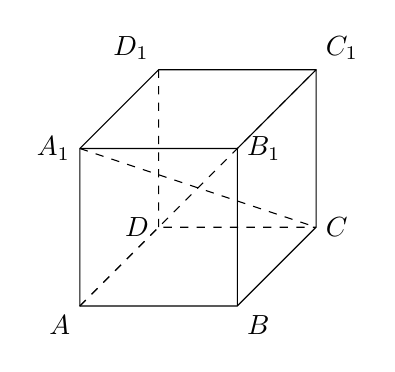
\begin{tikzpicture}
        \draw (0,0) node [below left] {$A$} coordinate (A) --++ (2,0) node [below right] {$B$} coordinate (B) --++ (45:{2*sqrt(2)/2}) node [right] {$C$} coordinate (C)
        --++ (0,2) node [above right] {$C_1$} coordinate (C1)
        --++ (-2,0) node [above left] {$D_1$} coordinate (D1) --++ (225:{2*sqrt(2)/2}) node [left] {$A_1$} coordinate (A1) -- cycle;
        \draw (A) ++ (2,2) node [right] {$B_1$} coordinate (B1) -- (B) (B1) --++ (45:{2*sqrt(2)/2}) (B1) --++ (-2,0);
        \draw [dashed] (A) --++ (45:{2*sqrt(2)/2}) node [left] {$D$} coordinate (D) --++ (2,0) (D) --++ (0,2);
        \draw [dashed] (A1) -- (C) (A) --(C1);
    \end{tikzpicture}
\end{center}
\item {\tiny (000755)}椭圆的长轴长等于$m$, 短轴长等于$n$, 则此椭圆的内接矩形的面积的最大值为\blank{50}.
\item {\tiny (000756)}已知集合$A=\{1,2,3\}B=\{1,m\}$, 若$3-m\in A$, 则非零实数$m$的数值是\blank{50}.
\item {\tiny (000757)}不等式$|1-x|>1$的解集是\blank{50}.
\item {\tiny (000758)}若函数$f(x)=\sqrt{8-ax-2x^2}$是偶函数, 则该函数的定义域是\blank{50}.
\item {\tiny (000759)}已知$\triangle ABC$的三内角$A,B,C$所对的边长分别为$a,b,c$, 若$a^2=b^2+c^2-2bc\sin A$, 则内角$A$的大小是\blank{50}.
\item {\tiny (000760)}已知向量$\overrightarrow a$在向量$\overrightarrow b$方向上的投影为$-2$, 且$|\overrightarrow b|=3$, 则$\overrightarrow a\cdot \overrightarrow b$=\blank{50}(结果用数值表示).
\item {\tiny (000761)}方程$\log_3(3 \cdot 2^x+5)-\log_3(4^x+1)=0$的解$x=$\blank{50}.
\item {\tiny (000762)}已知函数$f(x)=\begin{vmatrix}
2\sin x & -\cos 2x  \\ 1  & \cos x  \end{vmatrix}$, 则函数$f(x)$的单调递增区间是\blank{50}.
\item {\tiny (000763)}已知$\alpha$是实系数一元二次方程$x^2-(2m-1)x+m^2+1=0$的一个虚数根, 且$|\alpha|\le 2$, 则实数$m$的取值范围是\blank{50}.
\item {\tiny (000764)}已知某市$A$社区$35$岁至$45$岁的居民有$450$人, $46$岁至$55$岁的居民有$750$人, $56$岁至$65$岁的居民有$900$人. 为了解该社区$35$岁至$65$岁居民的身体健康状况, 社区负责人采用分层抽样技术抽取若干人进行体检调查, 若从$46$岁至$55$岁的居民中随机抽取了$50$人, 试问这次抽样调查抽取的人数是\blank{50}人.
\item {\tiny (000765)}将一枚质地均匀的硬币连续抛掷$5$次, 则恰好有$3$次出现正面向上的概率是\blank{50}(结果用数值表示).
\item {\tiny (000766)}函数$y=3\sin(2x+\dfrac{\pi}3)$的最小正周期T=\blank{50}.
\item {\tiny (000767)}函数$y=\lg x$的反函数是\blank{50}.
\item {\tiny (000768)}已知集合$P=\{x|(x+1)(x-3)<0\}$, $Q=\{x||x|>2\}$, 则$P\cap Q$=\blank{50}.
\item {\tiny (000769)}函数$y=x+\dfrac9x$, $x\in (0,+\infty)$的最小值是\blank{50}.
\item {\tiny (000770)}计算: $\displaystyle\lim_{n\to\infty}[\dfrac12+\dfrac14+\dfrac18+\cdots+(\dfrac12)^n]$=\blank{50}.
\item {\tiny (000771)}记球$O_1$和$O_2$的半径、体积分别为$r_1$、$V_1$和$r_2$、$V_2$, 若$\dfrac{V_1}{V_2}=\dfrac8{27}$, 则$\dfrac{r_1}{r_2}=$\blank{50}.
\item {\tiny (000772)}若某线性方程组对应的增广矩阵是$\begin{pmatrix} m & 4 & 2 \\ 1 & m & m \end{pmatrix}$, 且此方程组有唯一一组解, 则实数$m$的取值范围是\blank{50}.
\item {\tiny (000773)}若一个布袋中有大小、质地相同的三个黑球和两个白球, 从中任取两个球, 则取出的两球中恰是一个白球和一个黑球的概率是\blank{50}.
\item {\tiny (000774)}$(1+2x)^n$的二项展开式中, 含$x^3$项的系数等于含$x$项的系数的$8$倍, 则正整数$n=$\blank{50}.
\item {\tiny (000775)}平面上三条直线$x-2y+1=0$, $x-1=0$, $x+ky=0$, 如果这三条直线将平面划分为六个部分, 则实数$k$的取值组成的集合$A=$\blank{50}.
\item {\tiny (000776)}已知集合$A=\{1,3,5,7,9\}$, $B=\{0,1,2,3,4,5\}$, 则图中阴影部分集合用列举法表示的结果是\blank{50}.
\begin{center}
    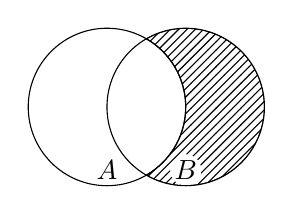
\begin{tikzpicture}
        \begin{scope}[even odd rule]
            \clip  (1,-0.8) circle (0.2) (1,0) circle (1);
            \filldraw [pattern = {north east lines}] (0.5,{0.5*sqrt(3)}) arc (60:-60:1) arc (-120:120:1);
        \end{scope}
        \draw (0,0) circle (1);
        \draw (1,0) circle (1);
        \draw (0,-0.8) node {$A$};
        \draw (1,-0.8) node {$B$};
    \end{tikzpicture}
\end{center}
\item {\tiny (000777)}若复数$z$满足$z(1-\mathrm{i})=2 \mathrm{i}$($\mathrm{i}$是虚数单位), 则$|z|=$\blank{50}.
\item {\tiny (000778)}函数$y=\sqrt{\lg(x+2)}$的定义域为\blank{50}.
\item {\tiny (000779)}在从$4$个字母$a$、$b$、$c$、$d$中任意选出$2$个不同字母的试验中, 其中含有字母$d$事件的概率是\blank{50}.
\item {\tiny (000780)}如图的三个直角三角形是一个体积为$20\text{cm}^3$的几何体的三视图, 则$h=$\blank{50}.
\begin{center}
    \begin{tikzpicture}[>=latex]
        \draw (0,0) -- (2.5,0) -- (0,2) -- cycle;
        \draw (0,-0.1) -- (0,-0.3) (2.5,-0.1) -- (2.5,-0.3);
        \draw (1.25,-0.2) node {$5$};
        \draw [->] (1.05,-0.2) -- (0,-0.2);
        \draw [->] (1.45,-0.2) -- (2.5,-0.2);
        \draw (1.25,-0.5) node {主视图};
        \draw (-0.1,0) -- (-0.3,0) (-0.1,2) -- (-0.3,2);
        \draw (-0.2,1) node {$h$};
        \draw [->] (-0.2,0.8) -- (-0.2,0);
        \draw [->] (-0.2,1.2) -- (-0.2,2);
        \draw (3.5,0) -- (6.5,0) -- (3.5,2) -- cycle;
        \draw (3.5,-0.1) -- (3.5,-0.3) (6.5,-0.1) -- (6.5,-0.3);
        \draw (5,-0.2) node {$6$};
        \draw [->] (4.8,-0.2) -- (3.5,-0.2);
        \draw [->] (5.2,-0.2) -- (6.5,-0.2);
        \draw (5,-0.5) node {左视图};
        \draw (0,-1) -- (2.5,-1) -- (0,-4) -- cycle;
        \draw (1.25,-4.5) node {俯视图};
    \end{tikzpicture}
\end{center}
\item {\tiny (000781)}如图, 以长方体$ABCD-A_1B_1C_1D_1$的顶点$D$为坐标原点, 过$D$的三条棱所在的直线为坐标轴, 建立空间直角坐标系, 若$\overrightarrow{DB_1}$的坐标为$(4,3,2)$, 则$\overrightarrow{BD_1}$的坐标为\blank{50}.
\begin{center}
    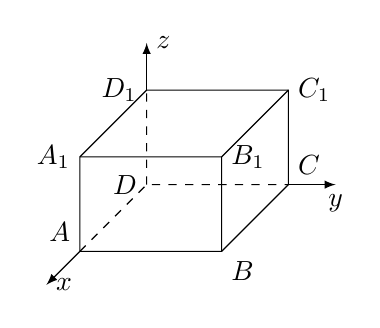
\begin{tikzpicture}[scale = 0.6, >=latex]
        \draw (0,0) node [above left] {$A$} coordinate (A) --++ (3,0) node [below right] {$B$} coordinate (B) --++ (45:{4/2}) node [above right] {$C$} coordinate (C)
        --++ (0,2) node [right] {$C_1$} coordinate (C1)
        --++ (-3,0) node [left] {$D_1$} coordinate (D1) --++ (225:{4/2}) node [left] {$A_1$} coordinate (A1) -- cycle;
        \draw (A) ++ (3,2) node [right] {$B_1$} coordinate (B1) -- (B) (B1) --++ (45:{4/2}) (B1) --++ (-3,0);
        \draw [dashed] (A) --++ (45:{4/2}) node [left] {$D$} coordinate (D) --++ (3,0) (D) --++ (0,2);
        \draw [->] (A) --++ (225:1) node [right] {$x$};
        \draw [->] (C) --++ (1,0) node [below] {$y$};
        \draw [->] (D1) --++ (0,1) node [right] {$z$};
    \end{tikzpicture}
\end{center}
\item {\tiny (000782)}方程$\cos 2x=-\dfrac{\sqrt3}2$的解集为\blank{50}.
\item {\tiny (000783)}已知抛物线的顶点在坐标原点, 焦点在$y$轴上, 抛物线上一点$M(a,-4) \ (a>0)$到焦点F的距离为$5$. 则该抛物线的标准方程为\blank{50}.
\item {\tiny (000784)}已知等比数列$\{a_n\}$的前$n$项和为$S_n$($n\in \mathbf{N}*$), 且$\dfrac{S_6}{S_3}=-\dfrac{19}8$,$a_4-a_2=-\dfrac{15}8$, 则$a_3$的值为\blank{50}.
\item {\tiny (000785)}在直角三角形$ABC$中, $\angle A=\dfrac{\pi}2$, $AB=3$, $AC=4$, $E$为三角形$ABC$内一点, 且$AE=\dfrac{\sqrt2}2$. 若$\overrightarrow{AE}=\lambda \overrightarrow{AB}+\mu \overrightarrow{AC}$, 则$3\lambda +4 \mu$的最大值等于\blank{50}.
\item {\tiny (000786)}双曲线$\dfrac{x^2}{a^2}-\dfrac{y^2}9=1 \ (a>0)$的渐近线方程为$3x\pm 2y=0$, 则$a=$\blank{50}.
\item {\tiny (000787)}若二元一次方程组的增广矩阵是$\begin{pmatrix} 1 & 2 & c_1  \\ 3 & 4 & c_2 \end{pmatrix}$, 其解为$\begin{cases} x=10, \\ y=0, \end{cases}$ 则$c_1+c_2=$\blank{50}.
\item {\tiny (000788)}设$m\in \mathbf{R}$, 若复数$(1+m\mathrm{i})(1+\mathrm{i})$在复平面内对应的点位于实轴上, 则$m=$\blank{50}.
\item {\tiny (000789)}定义在$\mathbf{R}$上的函数$f(x)=2^x-1$的反函数为$y=f^{-1}(x)$, 则$f^{-1}(3)=$\blank{50}.
\item {\tiny (000790)}直线$l$的参数方程为$\begin{cases}  x=1+t, \\ y=-1+2t, \end{cases}$($t$为参数), 则$l$的一个法向量为\blank{50}.
\item {\tiny (000791)}已知数列$\{a_n\}$, 其通项公式为$a_n=3n+1$, $n\in \mathbf{N}^*$, $\{a_n\}$的前$n$项和为$S_n$, 则$\displaystyle\lim_{n\to\infty}\dfrac{S_n}{n\cdot {a_n}}=$\blank{50}.
\item {\tiny (000792)}已知向量$\overrightarrow a$、$\overrightarrow b$的夹角为$60^{\circ}$, $|\overrightarrow a|=1$, $|\overrightarrow b|=2$, 若$(\overrightarrow a+2 \overrightarrow b)\perp (x\overrightarrow a-\overrightarrow b)$, 则实数$x$的值为\blank{50}.
\item {\tiny (000793)}若球的表面积为$100 \pi$, 平面$\alpha$与球心的距离为$3$, 则平面$\alpha$截球所得的圆面面积为\blank{50}.
\item {\tiny (000794)}若平面区域的点$(x,y)$满足不等式$\dfrac{|x|}k+\dfrac{|y|}4\le 1\ (k>0)$, 且$z=x+y$的最小值为$-5$, 则常数$k=$\blank{50}.
\item {\tiny (000795)}若函数$f(x)={\log_a}(x^2-ax+1)\ (a>0, \ a\ne 1)$没有最小值, 则$a$的取值范围是\blank{50}.
\item {\tiny (000796)}$\displaystyle\lim_{n\to \infty}\dfrac{2n+1}{n-1}=$\blank{50}.
\item {\tiny (000797)}不等式$\dfrac x{x-1}<0$的解集为\blank{50}.
\item {\tiny (000798)}已知$\{a_n\}$是等比数列, 它的前$n$项和为$S_n$, 且$a_3=4$, $a_4=-8$, 则$S_5=$\blank{50}.
\item {\tiny (000799)}已知$f^{-1}(x)$是函数$f(x)=\log_2(x+1)$的反函数, 则$f^{-1}(2)=$\blank{50}.
\item {\tiny (000800)}$(\sqrt x+\dfrac1x)^9$二项展开式中的常数项为\blank{50}.
\item {\tiny (000801)}椭圆$\begin{cases} x=2 \cos\theta, \\ y=\sqrt3\sin\theta  \end{cases}$($\theta$为参数)的右焦点为\blank{50}.
\item {\tiny (000802)}满足约束条件$\begin{cases} x+2y\le 4, \\ 2x+y\le 3, \\ x\ge 0, \\ y\ge 0 \end{cases}$的目标函数$f=3x+2y$的最大值为\blank{50}.
\item {\tiny (000803)}函数$f(x)=\cos^2 x+\dfrac{\sqrt3}2\sin 2x,\ x\in \mathbf{R}$的单调递增区间为\blank{50}.
\item {\tiny (000804)}已知抛物线型拱桥的顶点距水面$2$米时, 量得水面宽为$8$米. 当水面下降$1$米后, 水面的宽为\blank{50}米.
\item {\tiny (000805)}一个四面体的顶点在空间直角坐标系$O-xyz$中的坐标分别是$(0,0,0)$, $(1,0,1)$, $(0,1,1)$, $(1,1,0)$, 则该四面体的体积为\blank{50}.
\item {\tiny (000806)}抛物线$x^2=12y$的准线方程为\blank{50}.
\item {\tiny (000807)}若函数$f(x)=\dfrac1{x-2m+1}$是奇函数, 则实数$m=$\blank{50}.
\item {\tiny (000808)}若函数$f(x)=\sqrt{2x+3}$的反函数为$g(x)$, 则函数$g(x)$的零点为\blank{50}.
\item {\tiny (000809)}书架上有上、中、下三册的《白话史记》和上、下两册的《古诗文鉴赏辞典》, 现将这五本书从左到右摆放在一起, 则中间位置摆放中册《白话史记》的不同摆放种数为\blank{50}(结果用数值表示).
\item {\tiny (000810)}在锐角三角形$ABC$中, 角$A$、$B$、$C$的对边分别为$a$、$b$、$c$, 若$(b^2+c^2-a^2)\tan A=bc$, 则角$A$的大小为\blank{50}.
\item {\tiny (000811)}若$(x^3-\dfrac1{x^2})^n$的展开式中含有非零常数项, 则正整数$n$的最小值为\blank{50}.
\item {\tiny (000812)}某单位年初有两辆车参加某种事故保险, 对在当年内发生此种事故的每辆车, 单位均可获赔(假设每辆车最多只获一次赔偿). 设这两辆车在一年内发生此种事故的概率分别为$\dfrac1{20}$和$\dfrac1{21}$, 且各车是否发生事故相互独立, 则一年内该单位在此种保险中获赔的概率为\blank{50}(结果用最简分数表示).
\item {\tiny (000813)}在平面直角坐标系$xOy$中, 直线$l$的参数方程为$\begin{cases} x=\dfrac{\sqrt2}2t-\sqrt2, \\ y=\dfrac{\sqrt2}4t, \end{cases}$($t$为参数), 椭圆$C$的参数方程为$\begin{cases} x=\cos \theta,  \\ y=\dfrac12\sin \theta,  \end{cases}$($\theta$为参数), 则直线$l$与椭圆$C$的公共点坐标为\blank{50}.
\item {\tiny (000814)}设函数$f(x)=\log_m x$($m>0$且$m\ne 1$), 若$m$是等比数列$\{a_n\}$($n\in \mathbf{N}^*$)的公比, 且$f(a_2a_4a_6\cdots a_{2018})=7$, 则$f(a_1^2)+f(a_2^2)+f(a_3^2)+\cdots+f(a_{2018}^2)$的值为\blank{50}.
\item {\tiny (000815)}设变量$x,y$满足条件$\begin{cases}  x-y\ge 0, \\ 2x+y\le 2, \\ y\ge 0, \\ x+y\le m, \end{cases}$ 若该条件表示的平面区域是三角形, 则实数$m$的取值范围是\blank{50}.
\item {\tiny (000816)}不等式$|x-3|<2$的解集为\blank{50}.
\item {\tiny (000817)}若复数$z$满足$2 \overline z-3=1+5 \mathrm{i}$($\mathrm{i}$是虚数单位), 则$z=$\blank{50}.
\item {\tiny (000818)}若$\sin\alpha =\dfrac13$, 则$\cos(\alpha -\dfrac{\pi}2)=$\blank{50}.
\item {\tiny (000819)}已知两个不同向量$\overrightarrow{OA}=(1,m)$, $\overrightarrow{OB}=(m-1,2)$, 若$\overrightarrow{OA}\perp \overrightarrow{AB}$, 则实数$m=$\blank{50}.
\item {\tiny (000820)}在等比数列$\{a_n\}$中, 公比$q=2$, 前$n$项和为$S_n$, 若$S_5=1$, 则$S_{10}=$\blank{50}.
\item {\tiny (000821)}若$x,y$满足$\begin{cases}x\le 2, \\ x-y+1\ge 0, \\ x+y-2\ge 0,\end{cases}$ 则$z=2x-y$的最小值为\blank{50}.
\item {\tiny (000822)}如图所示, 一个圆柱的主视图和左视图都是边长为$1$的正方形,\blank{50}俯视图是一个直径为$1$的圆, 那么这个圆柱的体积为\blank{50}.
\begin{center}
    \begin{tikzpicture}
        \draw (0,0) rectangle (1.2,1.2) (1.8,0) rectangle (3,1.2);
        \draw (0.6,-0.3) node {主视图} (2.4,-0.3) node {左视图};
        \draw (0.6,-1.4) circle (0.6);
        \draw (0.6,-2.3) node {俯视图};
    \end{tikzpicture}
\end{center}
\item {\tiny (000823)}$(1+\dfrac1{x^2})(1+x)^6$展开式中$x^2$的系数为\blank{50}.
\item {\tiny (000824)}已知$f(x)$是定义在$[-2,2]$上的奇函数, 当$x\in (0,2]$时,$f(x)=2^x-1$, 函数$g(x)=x^2-2x+m$. 如果对于任意的$x_1\in [-2,2]$, 总存在$x_2\in [-2,2]$, 使得$f(x_1)\le g(x_2)$, 则实数$m$的取值范围是\blank{50}.
\item {\tiny (000825)}已知曲线$C:y=-\sqrt{9-x^2}$, 直线$l:y=2$, 若对于点$A(0,m)$, 存在$C$上的点$P$和$l$上的点$Q$, 使得$\overrightarrow{AP}+\overrightarrow{AQ}=\overrightarrow 0$, 则$m$取值范围是\blank{50}.
\item {\tiny (000826)}函数$y=\lg x-1$的零点是\blank{50}.
\item {\tiny (000827)}计算:$\displaystyle\lim_{n\to\infty}\dfrac{2n}{4n+1}=$\blank{50}.
\item {\tiny (000828)}若$(1+3x)^n$的二项展开式中$x^2$项的系数是$54$, 则$n=$\blank{50}.
\item {\tiny (000829)}掷一颗均匀的骰子, 出现奇数点的概率为\blank{50}.
\item {\tiny (000830)}若$x,y$满足$\begin{cases} x-y\ge 0, \\ x+y\le 2, \\ y\ge 0, \end{cases}$ 则目标函数$f=x+2y$的最大值为\blank{50}.
\item {\tiny (000831)}若复数$z$满足$|z|=1$, 则$|z-\mathrm{i}|$的最大值是\blank{50}.
\item {\tiny (000832)}若一个圆锥的主视图(如图所示)是边长为$3,3,2$的三角形, 则该圆锥的体积是\blank{50}.
\begin{center}
    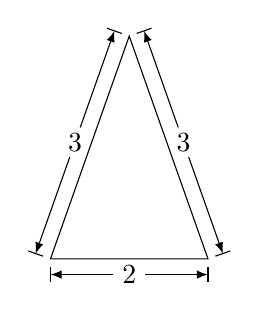
\begin{tikzpicture}[>=latex]
        \draw (-1,0) -- (1,0) -- (0,{2*sqrt(2)}) -- cycle;
        \draw (-1,-0.1) -- (-1,-0.3) (1,-0.1) -- (1,-0.3);
        \draw (0,-0.2) node {$2$};
        \draw [->] (-0.2,-0.2) -- (-1,-0.2);
        \draw [->] (0.2,-0.2) -- (1,-0.2);
        \draw (1,0) ++ ({asin(1/3)}:0.1) --++ ({asin(1/3)}:0.2);
        \draw (0,{2*sqrt(2)}) ++ ({asin(1/3)}:0.1) --++ ({asin(1/3)}:0.2);
        \draw [->] ($(1,0)!{1.3/3}!(0,{2*sqrt(2)})$) ++ ({asin(1/3)}:0.2) --++ ({-acos(1/3)}:1.3);
        \draw [->] ($(1,0)!{1.7/3}!(0,{2*sqrt(2)})$) ++ ({asin(1/3)}:0.2) --++ ({180-acos(1/3)}:1.3);
        \draw ($(1,0)!{0.5}!(0,{2*sqrt(2)})$) ++ ({asin(1/3)}:0.2) node {$3$};
        \draw (-1,0) ++ ({180-asin(1/3)}:0.1) --++ ({180-asin(1/3)}:0.2);
        \draw (0,{2*sqrt(2)}) ++ ({180-asin(1/3)}:0.1) --++ ({180-asin(1/3)}:0.2);
        \draw [->] ($(-1,0)!{1.3/3}!(0,{2*sqrt(2)})$) ++ ({180-asin(1/3)}:0.2) --++ ({180+acos(1/3)}:1.3);
        \draw [->] ($(-1,0)!{1.7/3}!(0,{2*sqrt(2)})$) ++ ({180-asin(1/3)}:0.2) --++ ({acos(1/3)}:1.3);
        \draw ($(-1,0)!{0.5}!(0,{2*sqrt(2)})$) ++ ({180-asin(1/3)}:0.2) node {$3$};
    \end{tikzpicture}
\end{center}
\item {\tiny (000833)}若双曲线$\dfrac{x^2}3-\dfrac{16y^2}{p^2}=1\ (p>0)$的左焦点在抛物线$y^2=2px$的准线上, 则$p=$\blank{50}.
\item {\tiny (000834)}若$\sin(x-y)\cos x-\cos(x-y)\sin x=\dfrac35$, 则$\tan 2y$的值为\blank{50}.
\item {\tiny (000835)}若$\{a_n\}$为等比数列, $a_n>0$, 且$a_{2018}=\dfrac{\sqrt2}2$, 则$\dfrac1{a_{2017}}+\dfrac2{a_{2019}}$的最小值为\blank{50}.
\item {\tiny (000836)}已知集合$A=\{1,2,m\}$,$B=\{2,4\}$, 若$A\cup B=\{1,2,3,4\}$, 则实数$m=$\blank{50}.
\item {\tiny (000837)}$(x+\dfrac1x)^n$的展开式中的第$3$项为常数项, 则正整数$n=$\blank{50}.
\item {\tiny (000838)}已知复数$z$满足${z^2}=4+3\mathrm{i}$($\mathrm{i}$为虚数单位), 则$|z|=$\blank{50}.
\item {\tiny (000839)}已知平面直角坐标系$xOy$中动点$P(x,y)$到定点$(1,0)$的距离等于$P$到定直线$x=-1$的距离, 则点$P$的轨迹方程为\blank{50}.
\item {\tiny (000840)}已知数列$\{a_n\}$是首项为$1$, 公差为$2$的等差数列,$S_n$是其前$n$项和, 则$\displaystyle\lim_{n\to\infty}\dfrac{S_n}{a_n^2}=$\blank{50}.
\item {\tiny (000841)}设变量$x,y$满足条件$\begin{cases} x\ge 1, \\ x+y-4\le 0, \\  x-3y+4\le 0,  \end{cases}$ 则目标函数$z=3x-y$的最大值为\blank{50}.
\item {\tiny (000842)}将圆心角为$\dfrac{2\pi}3$, 面积为$3\pi$的扇形围成一个圆锥的侧面, 则此圆锥的体积为\blank{50}.
\item {\tiny (000843)}三棱锥$P-ABC$及其三视图中的主视图和左视图如图所示, 则棱$PB$的长为\blank{50}.
\begin{center}
    \begin{tikzpicture}[>=latex]
        \draw (0,0) node [right] {$C$} coordinate (C) -- (0,2) node [above] {$P$} coordinate (P) -- (-2,0) node [left] {$A$} coordinate (A);
        \draw (-1,0) ++ (-135:{sqrt(3)/2}) node [below] {$B$} coordinate (B) -- (A) (B) -- (C) (B) -- (P);
        \draw [dashed] (A) -- (C);
        \draw (2,0) -- (4,0) -- (4,2) -- cycle;
        \draw (3,0) -- (4,2);
        \draw (5,0) -- ({5+sqrt(3)},0) coordinate (D) -- (5,2) -- cycle;
        \draw (2,-0.1) -- (2,-0.3) (3,-0.1) -- (3,-0.3) (4,-0.1) -- (4,-0.3);
        \draw [->] (2.2,-0.2) -- (2,-0.2);
        \draw [->] (2.8,-0.2) -- (3,-0.2);
        \draw [->] (3.2,-0.2) -- (3,-0.2);
        \draw [->] (3.8,-0.2) -- (4,-0.2);
        \draw (2.5,-0.2) node {$2$} (3.5,-0.2) node {$2$};
        \draw (3,-0.7) node {主视图};
        \draw (5,-0.1) -- (5,-0.3) (D) ++ (0,-0.1) --++ (0,-0.2);
        \draw [->] ({5+sqrt(3)/2-0.4},-0.2) -- (5,-0.2);
        \draw [->] ({5+sqrt(3)/2+0.4},-0.2) -- ({5+sqrt(3)},-0.2);
        \draw ({5+sqrt(3)/2},-0.2) node {$2\sqrt{3}$};
        \draw ({5+sqrt(3)/2},-0.7) node {主视图};
        \draw (4.9,0) -- (4.7,0) (4.9,2) -- (4.7,2);
        \draw [->] (4.8,0.8) -- (4.8,0);
        \draw [->] (4.8,1.2) -- (4.8,2);
        \draw (4.8,1) node {$4$};
    \end{tikzpicture}
\end{center}
\item {\tiny (000844)}某商场举行购物抽奖促销活动, 规定每位顾客从装有编号为$0$、$1$、$2$、$3$的四个相同小球的抽奖箱中, 每次取出一球记下编号后放回, 连续取两次, 若取出的两个小球编号相
加之和等于$6$, 则中一等奖, 等于$5$中二等奖, 等于$4$或$3$中三等奖. 则顾客抽奖中三等奖的概率为\blank{50}.
\item {\tiny (000845)}已知函数$f(x)=\lg (\sqrt{x^2+1}+ax)$的定义域为$\mathbf{R}$, 则实数$a$的取值范围是\blank{50}.
\item {\tiny (000846)}已知全集$U=\mathbf{R}$,若集合$A=\{x|\dfrac x{x-1}>0\}$, 则$\complement_U A=$\blank{50}.
\item {\tiny (000847)}已知复数$z$满足$z\cdot (1-\mathrm{i})=2\mathrm{i}$, 其中$\mathrm{i}$为虚数单位, 则$|z|=$\blank{50}.
\item {\tiny (000848)}双曲线$2 x^2-y^2=6$的焦距为\blank{50}.
\item {\tiny (000849)}已知$(ax+\dfrac1x)^6$二项展开式中的第五项系数为$\dfrac{15}2$, 则正实数$a$\blank{50}.
\item {\tiny (000850)}方程$\log_2(9^x+7)=2+\log_2(3^x+1)$的解为\blank{50}.
\item {\tiny (000851)}已知函数$f(x)=\dfrac{3x+1}{x+a}\ (a\ne \dfrac13)$的图像与它的反函数的图像重合, 则实数$a$的值为\blank{50}.
\item {\tiny (000852)}在$\triangle ABC$中, 边$a,b,c$所对角分别为$A,B,C$, 若$\begin{vmatrix} a & \sin (\dfrac{\pi}2+B)  \\ b & \cos A  \end{vmatrix}=0$, 则$\triangle ABC$的形状为\blank{50}.
\item {\tiny (000853)}若某几何体的三视图(单位:$\text{cm}$)如图所示, 则此几何体的体积是\blank{50}$\text{cm}^3$.
\begin{center}
    \begin{tikzpicture}[>=latex,scale = 0.7]
        \draw (1,0) -- (2,0) -- (2,3) -- (3,3) -- (3,4) -- (0,4) -- (0,3) -- (1,3) -- cycle;
        \draw (5,0) -- (8,0) -- (8,4) -- (5,4) -- cycle (5,3) -- (8,3);
        \draw (0,-1) -- (0,-4) -- (3,-4) -- (3,-1) -- cycle;
        \draw [dashed] (1,-1) -- (1,-4) (2,-1) -- (2,-4);
        \draw (1.5,-4.5) node {俯视图} (1.5,-0.5) node {主视图} (6.5,-0.5) node {俯视图};
        \draw (3.1,-4) -- (3.3,-4) (3.1,-1) -- (3.3,-1);
        \draw [->] (3.2,-2.1) -- (3.2,-1);
        \draw [->] (3.2,-2.9) -- (3.2,-4);
        \draw (3.2,-2.5) node {$3$};
        \draw (5,4.1) -- (5,4.3) (8,4.1) -- (8,4.3);
        \draw [->] (6.1,4.2) -- (5,4.2);
        \draw [->] (6.9,4.2) -- (8,4.2);
        \draw (6.5,4.2) node {$3$};
        \draw (0,4.1) -- (0,4.3) (1,4.1) -- (1,4.3) (2,4.1) -- (2,4.3) (3,4.1) -- (3,4.3);
        \draw [->] (0.3,4.2) -- (0,4.2);
        \draw [->] (0.7,4.2) -- (1,4.2);
        \draw (0.5,4.2) node {$1$};
        \draw [->] (1.3,4.2) -- (1,4.2);
        \draw [->] (1.7,4.2) -- (2,4.2);
        \draw (1.5,4.2) node {$1$};
        \draw [->] (2.3,4.2) -- (2,4.2);
        \draw [->] (2.7,4.2) -- (3,4.2);
        \draw (2.5,4.2) node {$1$};
        \draw (3.1,4) -- (3.3,4) (3.1,3) -- (3.3,3) (3.1,0) -- (3.3,0);
        \draw [->] (3.2,1.1) -- (3.2,0);
        \draw [->] (3.2,1.9) -- (3.2,3);
        \draw (3.2,1.5) node {$3$};
        \draw [->] (3.2,3.2) -- (3.2,3);
        \draw [->] (3.2,3.8) -- (3.2,4);
        \draw (3.2,3.5) node {$1$};
    \end{tikzpicture}
\end{center}
\item {\tiny (000854)}已知四面体$ABCD$中, $AB=CD=2$, $E$, $F$分别为$BC$, $AD$的中点, 且异面直线$AB$与$CD$所成的角为$\dfrac{\pi}3$, 则$EF$=\blank{50}.
\item {\tiny (000855)}设$m,n$分别为连续两次投掷骰子得到的点数, 且向量$\overrightarrow a=(m,n)$,$\overrightarrow b=(1,-1)$, 则$\overrightarrow a$与$\overrightarrow b$的夹角为锐角的概率是\blank{50}.
\item {\tiny (000856)}已知数列$\{a_n\}$的通项公式为$a_n={(-1)}^n\cdot n+2^n, \ n\in \mathbf{N}^*$, 则这个数列的前$2n$项和$S_{2n}=$\blank{50}.
\item {\tiny (000857)}设集合$A=\{x||x|<2,\ x\in \mathbf{R}\}$, $B=\{x|x^2-4x+3\ge 0, \ x\in \mathbf{R}\}$, 则$A\cap B=$\blank{50}.
\item {\tiny (000858)}已知$\mathrm{i}$为虚数单位, 复数$z$满足$\dfrac{1-z}{1+z}=\mathrm{i}$, 则$|z|=$\blank{50}.
\item {\tiny (000859)}设$a>0$且$a\ne 1$, 若函数$f(x)=a^{x-1}+2$的反函数的图像经过定点$P$, 则点$P$的坐标是\blank{50}.
\item {\tiny (000860)}计算: $\displaystyle\lim_{n\to\infty}\dfrac{\mathrm{P}_n^2+\mathrm{C}_n^2}{(n+1)^2}=$\blank{50}.
\item {\tiny (000861)}在平面直角坐标系内, 直线$l:2x+y-2=0$, 将$l$与两条坐标轴围成的封闭图形绕$y$轴旋转一周, 所得几何体的体积为\blank{50}.
\item {\tiny (000862)}已知$\sin 2\theta +\sin\theta =0$,$\theta \in (\dfrac{\pi}2,\pi)$, 则$\tan 2\theta =$\blank{50}.
\item {\tiny (000863)}设定义在$\mathbf{R}$上的奇函数$y=f(x)$, 当$x>0$时, $f(x)=2^x-4$, 则不等式$f(x)\le 0$的解集是\blank{50}.
\item {\tiny (000864)}在平面直角坐标系$xOy$中, 有一定点$A(1,1)$, 若线段$OA$的垂直平分线过抛物线$C:y^2=2px \ (p>0)$的焦点, 则抛物线$C$的方程为\blank{50}.
\item {\tiny (000865)}曲线$\begin{cases} x=1-\dfrac{\sqrt5}5 t, \\ y=-1+\dfrac{2\sqrt5}5t, \end{cases}$($t$为参数)与曲线$\begin{cases} x=\sin \theta \cdot \cos \theta, \\ y=\sin \theta +\cos \theta,  \end{cases}$($\theta$为参数)的公共点的坐标为\blank{50}.
\item {\tiny (000866)}记$(2x+\dfrac1x)^n \ (n\in \mathbf{N}^*$)的展开式中第$m$项的系数为$b_m$, 若$b_3=2b_4$, 则$n=$\blank{50}.
\item {\tiny (000867)}已知各项均为正数的数列$\{a_n\}$满足$\sqrt{a_1}+\sqrt{a_2}+\cdots+\sqrt{a_n}=n^2+3n$($n\in \mathbf{N}^*$), 则$\dfrac{a_1}2+\dfrac{a_2}3+\cdots \dfrac{a_n}{n+1}=$\blank{50}.
\item {\tiny (000868)}函数$f(x)=\dfrac{\sqrt{x+2}}{x-1}$的定义域为\blank{50}.
\item {\tiny (000869)}已知线性方程组的增广矩阵为$\begin{pmatrix} 1 & -1  & 3  \\ a & 3 & 4 \end{pmatrix}$, 若该线性方程组的解为$\begin{pmatrix} -1 \\ 2\end{pmatrix}$, 则实数$a=$\blank{50}.
\item {\tiny (000870)}计算$\displaystyle\lim_{n\to\infty}\dfrac{1+2+3+\cdots +n}{n^2+1}=$\blank{50}.
\item {\tiny (000871)}若向量$\overrightarrow a$、$\overrightarrow b$满足$|\overrightarrow a|=1$, $|\overrightarrow b|=2$, 且$\overrightarrow a$与$\overrightarrow b$的夹角为$\dfrac{\pi}3$, 则$|\overrightarrow a+\overrightarrow b|=$\blank{50}.
\item {\tiny (000872)}若复数$z_1=3+4\mathrm{i}$, $z_2=1-2\mathrm{i},$ 其中$\mathrm{i}$是虚数单位, 则复数$\dfrac{|z_1|}{\mathrm{i}}+\overline{z_2}$的虚部为\blank{50}.
\item {\tiny (000873)}$(\dfrac1x-\sqrt x)^6$的展开式中, 常数项为\blank{50}.
\item {\tiny (000874)}已知$\triangle  ABC$的内角$A$、$B$、$C$所对应边的长度分别为$a$、$b$、$c$, 若$\begin{vmatrix}a & c \\ c & a\end{vmatrix} = \begin{vmatrix}-b & -a \\ b & b\end{vmatrix}$, 则角$C$的大小是\blank{50}.
\item {\tiny (000875)}已知等比数列$\{a_n\}$的各项均为正数, 且满足:$a_1a_7=4$, 则数列$\{\log_2a_n\}$的前$7$项之和为\blank{50}.
\item {\tiny (000876)}已知双曲线$x^2-\dfrac{y^2}4=1$的右焦点为$F$, 过点$F$且平行于双曲线的一条渐近线的直线与双曲线交于点$P$, $M$在直线$PF$上, 且满足$\overrightarrow{OM}\cdot \overrightarrow{PF}=0$, 则$\dfrac{|\overrightarrow{PM}|}{|\overrightarrow{PF}|}=$\blank{50}.
\item {\tiny (000877)}现有$5$位教师要带$3$个班级外出参加志愿者服务, 要求每个班级至多两位老师带队, 且教师甲、乙不能单独带队, 则不同的带队方案有\blank{50}(用数字作答).
\item {\tiny (000878)}抛物线$y^2=4x$的焦点坐标是\blank{50}.
\item {\tiny (000879)}若集合$A=\{x|3x+1>0\}$, $B=\{x||x-1|<2\}$, 则$A\cap B$=\blank{50}.
\item {\tiny (000880)}若$\overrightarrow d=(3,2)$是直线$l$的一个方向向量, 则$l$的倾斜角的大小为\blank{50}(结果用反三角函数值表示).
\item {\tiny (000881)}若复数$z$满足$\dfrac{1-\mathrm{i}}z=-\mathrm{i}$, 其中$\mathrm{i}$为虚数单位, 则$z=$\blank{50}.
\item {\tiny (000882)}求值:$\begin{vmatrix}\arcsin\dfrac{\sqrt3}2 & 2  \\ \arctan\dfrac{\sqrt3}3 & 3  \end{vmatrix}$=\blank{50}弧度.
\item {\tiny (000883)}已知$\overrightarrow{AB}=3\overrightarrow{AP}$, 设$\overrightarrow{BP}=\lambda \overrightarrow{PA}$, 则实数$\lambda=$\blank{50}.
\item {\tiny (000884)}函数$y=\sqrt{x^2+2}+\dfrac1{\sqrt{x^2+2}}$的最小值为\blank{50}.
\item {\tiny (000885)}试写出$(x-\dfrac1x)^7$展开式中系数最大的项\blank{50}.
\item {\tiny (000886)}已知三个球的表面积之比是$1:2:3$, 则这三个球的体积之比为\blank{50}.
\item {\tiny (000887)}已知实数$x,y$满足$\begin{cases}x+y\ge 2, \\ x-y\le 2, \\ 0 \le y\le 3, \end{cases}$ 则目标函数$z=-\dfrac32x-y$的最大值为\blank{50}.
\item {\tiny (000888)}若不等式$x^2-5x+6<0$的解集为$(a,b)$, 则$\displaystyle\lim_{n\to\infty}\dfrac{a^n-2b^n}{3a^n-4b^n}=$\blank{50}.
\item {\tiny (000889)}从集合$A=\{1,2,3,4,5,6,7,8,9,10\}$中任取两个数, 欲使取到的一个数大于$k$, 另一个数小于$k$(其中$k\in A$)的概率是$\dfrac25$, 则$k=$\blank{50}.
\item {\tiny (000890)}设函数$f(x)=a^x+a^{-x}  \ (a>0, \ a\ne 1)$, 且$f(1)=3$, 则$f(0)+f(1)+f(2)$的值是\blank{50}.
\item {\tiny (000891)}已知集合$A=\{x||x-2|<a\}$, $B=\{x|x^2-2x-3<0\}$, 若$B\subseteq A$, 则实数$a$的取值范围是\blank{50}.
\item {\tiny (000892)}如果复数$z$满足$|z|=1$且$z^2=a+b\mathrm{i}$, 其中$a,b\in \mathbf{R}$, 则$a+b$的最大值是\blank{50}.
\item {\tiny (000893)}已知$x,y$满足$\begin{cases}
   x-y+5 \ge 0, \\ x+y\ge 0, \\ x\le 3, \end{cases}$ 若使得$z=ax+y$取最大值的点$(x,y)$有无数个, 则$a$的值等于\blank{50}.
\item {\tiny (000894)}在直角坐标系$xOy$中, 已知三点$A(a,1),B(2,b),C(3,4)$, 若向量$\overrightarrow{OA}$, $\overrightarrow{OB}$在向量$\overrightarrow{OC}$方向上的投影相同, 则$3a-4b$的值是\blank{50}.
\item {\tiny (000895)}已知$F_1,F_2$是椭圆$C:\dfrac{x^2}{a^2}+\dfrac{y^2}{b^2}=1\ (a>b>0)$的两个焦点, $P$为椭圆上一点, 且$\overrightarrow{PF_1}\perp \overrightarrow{PF_2}$, 若$\triangle PF_1F_2$的面积为$9$, 则$b=$\blank{50}.
\item {\tiny (000896)}$\triangle ABC$中,$a,b,c$分别是$\angle A,\angle B,\angle C$的对边且$ac+c^2=b^2-a^2$, 若$\triangle ABC$最大边长是$\sqrt7$且$\sin C=2\sin A$, 则$\triangle ABC$最小边的边长为\blank{50}.
\item {\tiny (000897)}设等差数列$\{a_n\}$的公差为$d$, 若$a_1,a_2,a_3,a_4,a_5,a_6,a_7$的方差为$1$, 则$d$=\blank{50}.
\item {\tiny (000898)}已知函数$f(x)=\begin{cases} \cos \dfrac{\pi x}2, & |x|\le 1,  \\ x^2-1, & |x|>1,  \end{cases}$ 则关于$x$的方程$f^2(x)-3f(x)+2=0$的实根的个数是\blank{50}个.
\item {\tiny (000899)}设集合$M=\{x|x^2=x\}$, $N=\{x|\log_2 x\le 0\}$, 则$M\cup N=$\blank{50}.
\item {\tiny (000900)}已知虚数$1+2\mathrm{i}$是方程$x^2+ax+b=0 (a\,b\in \mathbf{R})$的一个根, 则$a+b=$\blank{50}.
\item {\tiny (000901)}在报名的$5$名男生和$4$名女生中, 选取$5$人参加志愿者服务, 要求男、女生都有, 则不同的选取方式的种数为\blank{50}(结果用数值表示).
\item {\tiny (000902)}已知复数$z$在复平面上对应的点在曲线$y=\dfrac 2 x$上运动, 则$|z|$的最小值等于\blank{50}.
\item {\tiny (000903)}在正项等比数列$\{a_n\}$中, $a_1a_3=1$, $a_2+a_3=\dfrac43$, 则$\displaystyle\lim_{n\to\infty}(a_1+a_2+\cdots +a_n)=$\blank{50}.
\item {\tiny (000904)}已知$f(x)=2 \sin \omega x\ (\omega >0)$在$[0,\dfrac\pi 3]$单调递增, 则实数$\omega$的最大值为\blank{50}.
\item {\tiny (000905)}若行列式$\begin{vmatrix}   1 & 2 & 4 \\   \cos (\pi +x) & 2 & 0 \\   -1 & 1 & 6 \end{vmatrix}$中的元素$4$的代数余子式的值等于$\dfrac32$, 则实数$x$的取值集合为\blank{50}.
\item {\tiny (000906)}若二项式$(2x-\dfrac1{\sqrt x})^n$展开式中的第$5$项为常数项, 则展开式中各项的二项式系数之和为\blank{50}.
\item {\tiny (000907)}已知$A$、$B$是球$O$的球面上两点, $\angle AOB=90^\circ$, $C$为该球面上的动点, 若三棱锥$O-ABC$体积的最大值为$\dfrac{32}{3}$, 则球$O$的表面积为\blank{50}.
\begin{center}
    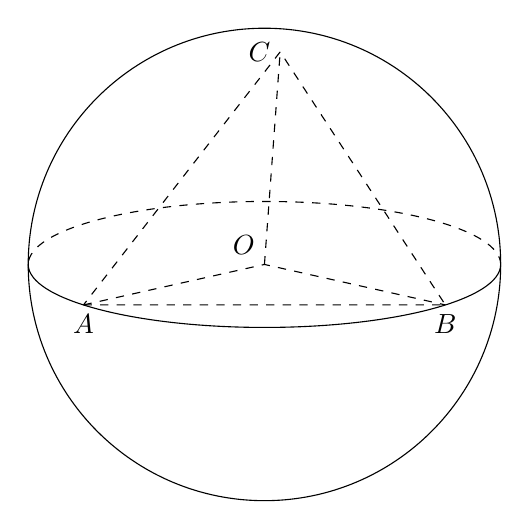
\begin{tikzpicture}
        \draw (0,0) circle (3);
        \draw (-3,0) arc (180:360:3 and 0.8);
        \draw [dashed] (3,0) arc (0:180:3 and 0.8);
        \draw ({3*cos(-140)},{0.8*sin(-140)}) coordinate (A) node [below] {$A$};
        \draw ({3*cos(-40)},{0.8*sin(-40)}) coordinate (B) node [below] {$B$};
        \draw (0.2,2.7) coordinate (C) node [left] {$C$};
        \draw (0,0) coordinate (O) node [above left] {$O$};
        \draw [dashed] (A) -- (B) -- (C) -- cycle;
        \draw [dashed] (A) -- (O) -- (B) (O) -- (C);
    \end{tikzpicture}
\end{center}
\item {\tiny (000908)}如图, $A$、$B$为椭圆$\dfrac{x^2}{a^2}+\dfrac{y^2}{b^2}=1 \ (a>b>0)$的两个顶点, 过椭圆的右焦点$F$作$x$轴的垂线, 与其交于点$C$. 若$AB\parallel OC$($O$为坐标原点), 则直线$AB$的斜率为\blank{50}.
\begin{center}
    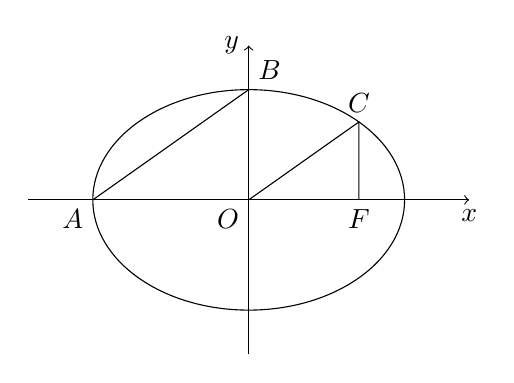
\begin{tikzpicture}[scale = 1.4]
        \draw [->] (-2,0) -- (2,0) node [below] {$x$};
        \draw [->] (0,-1.4) -- (0,1.4) node [left] {$y$};
        \draw (0,0) node [below left] {$O$};
        \draw (0,0) ellipse ({sqrt(2)} and 1);
        \draw (1,0) node [below] {$F$} -- (1,{sqrt(2)/2}) node [above] {$C$} -- (0,0);
        \draw ({-sqrt(2)},0) node [below left] {$A$} -- (0,1) node [above right] {$B$};
    \end{tikzpicture}
\end{center}
\item {\tiny (000909)}若经过抛物线 $y^2=4x$焦点的直线$l$与圆$(x-4)^2+y^2=4$相切, 则直线$l$的方程为\blank{50}.
\item {\tiny (000910)}若集合$A=\{x|y=\sqrt{x-1},\ x\in \mathbf{R}\}$, $B=\{x||x|\le 1,\ x\in \mathbf{R}\}$, 则$A\cap B=$\blank{50}.
\item {\tiny (000911)}若函数$f(x)=1+\dfrac1x$($x>0$)的反函数为$f^{-1}(x)$, 则不等式$f^{-1}(x)>2$的解集为\blank{50}.
\item {\tiny (000912)}若$\sin \alpha =\dfrac35$且$\alpha$是第二象限角, 则$\tan(\alpha -\dfrac\pi 4)=$\blank{50}.
\item {\tiny (000913)}若函数$f(x)$是定义在$\mathbf{R}$上的奇函数, 且满足$f(x+2)=-f(x)$, 则$f(2016)=$\blank{50}.
\item {\tiny (000914)}在$(x^3-\dfrac1x)^8$的展开式中, 其常数项的值为\blank{50}.
\item {\tiny (000915)}若函数$f(x)=\sin 2x$, $g(x)=f(x+\dfrac\pi 6)$, 则函数$g(x)$的单调递增区间为\blank{50}.
\item {\tiny (000916)}设$P$是曲线$\begin{cases} x=\dfrac{\sqrt2}2\sec \theta, \\ y=\tan \theta \end{cases}$($\theta $为参数)上的一动点, $O$为坐标原点, $M$为线段$OP$的中点, 则点$M$的轨迹的普通方程为\blank{50}.
\item {\tiny (000917)}不等式组$\begin{cases} x\le 3, \\ x+y\ge 0, \\ x-y+2 \ge 0 \end{cases}$所表示的区域的面积为\blank{50}.
\item {\tiny (000918)}若函数$f(x)=\log _5 x$($x>0$), 则方程$f(x+1)+f(x-3)=1$的解$x=$\blank{50}.
\item {\tiny (000919)}如图所示, 三个边长为$2$的等边三角形有一条边在同一直线上, 边$B_3C_3$上有$10$个不同的点$P_1,P_2,\cdots,P_{10}$, 记$M_i=\overrightarrow{AB_2}\cdot \overrightarrow{AP_i}$($i=1,2,\cdots,10$), 则$M_1+M_2+\cdots+M_{10}=$\blank{50}.
\begin{center}
    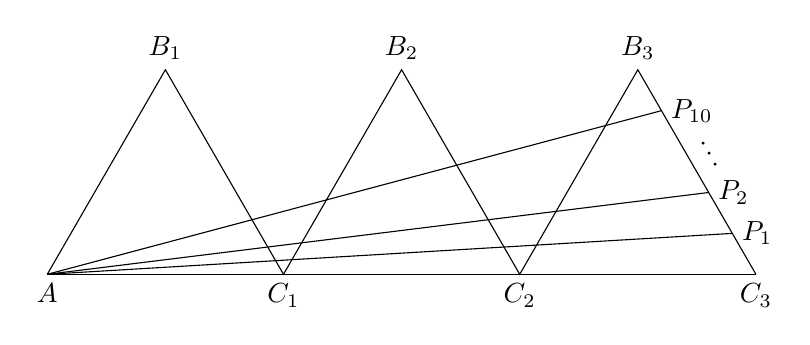
\begin{tikzpicture}[scale = 3]
        \draw (0,0) node [below] {$A$} -- (1,0) node [below] {$C_1$} -- (2,0) node [below] {$C_2$} -- (3,0) node [below] {$C_3$};
        \draw (3,0) -- (2.5,{sqrt(3)/2}) node [above] {$B_3$} -- (2,0) -- (1.5,{sqrt(3)/2}) node [above] {$B_2$} -- (1,0) -- (0.5,{sqrt(3)/2}) node [above] {$B_1$} -- (0,0);
        \draw ($(3,0)!0.2!(2.5,{sqrt(3)/2})$) coordinate (P1) node [right] {$P_1$} -- (0,0);
        \draw ($(3,0)!0.4!(2.5,{sqrt(3)/2})$) coordinate (P2) node [right] {$P_2$} -- (0,0);
        \draw ($(3,0)!0.8!(2.5,{sqrt(3)/2})$) coordinate (P3) node [right] {$P_{10}$} -- (0,0);
        \draw ($(3,0)!0.6!(2.5,{sqrt(3)/2})$) node [right] {\rotatebox{120}{$\cdots$}};
    \end{tikzpicture}
\end{center}
\item {\tiny (000920)}已知全集$U=\mathbf{R}$, $A=\{x|x^2-2x<0\}$, $B=\{x|x\ge 1\}$, 则$A\cap \complement_U B=$\blank{50}.
\item {\tiny (000921)}若函数$y=\cos ^2 \omega x$($\omega >0$)的最小正周期是$\pi$, 则$\omega=$\blank{50}.
\item {\tiny (000922)}圆$C:x^2+y^2-2x-4y+4=0$的圆心到直线$3x+4y+4=0$的距离$d=$\blank{50}.
\item {\tiny (000923)}已知圆锥的母线长为$5\text{cm}$, 侧面积为$15 \pi \text{cm}^2$, 则此圆锥的体积为\blank{50}$\text{cm}^3$.
\item {\tiny (000924)}已知$x,y\in \mathbf{R}^+$, 且满足$\dfrac x3+\dfrac y4=1$, 则$xy$的最大值为\blank{50}.
\item {\tiny (000925)}已知双曲线$\dfrac{x^2}{a^2}-\dfrac{y^2}{b^2}=1 \ (a>0,\ b>0)$的一条渐近线方程是$y=\sqrt3x$, 它的一个焦点与抛物线$y^2=16x$的焦点相同, 则双曲线的标准方程为\blank{50}.
\item {\tiny (000926)}已知函数$f(x)=\begin{cases}2^x +a, & x\ge 0, \\ x^2-ax, & x<0.\end{cases}$ 若$f(x)$的最小值是$a$, 则$a=$\blank{50}.
\item {\tiny (000927)}从$6$名男医生和$3$名女医生中选出$5$人组成一个医疗小组, 若这个小组中必须男女医生都有, 共有\blank{50}种不同的组建方案(结果用数值表示).
\item {\tiny (000928)}若数列$\{a_n\}$是首项为$1$, 公比为$a-\dfrac32$的无穷等比数列, 且$\{a_n\}$各项的和为$a$, 则$a$的值是\blank{50}.
\item {\tiny (000929)}设$a\ne 0$, $n$是大于$1$的自然数, $(1+\dfrac xa)^n$的展开式为$a_0+a_1x+a_2x^2+\cdots+a_nx^n$. 若$a_1=3$, $a_2=4$, 则$a=$\blank{50}.
\item {\tiny (000930)}矩形$ABCD$中, $AB=2$, $AD=1$, $P$为矩形内部一点, 且$AP=1$. 若$\overrightarrow{AP}=\lambda \overrightarrow{AB}+\mu \overrightarrow{AD} \ (\lambda,\ \mu \in \mathbf{R})$, 则$2 \lambda +\sqrt3\mu$的最大值是\blank{50}.
\item {\tiny (000931)}函数$y=\log_3 (x-1)$的定义域是\blank{50}.
\item {\tiny (000932)}集合$A=\{x|x^2-3x<0\}$, $B=\{x||x|<2\}$, 则$A\cup B$等于\blank{50}.
\item {\tiny (000933)}若复数$\dfrac{1+\mathrm{i}}{1-\mathrm{i}}+\dfrac12b$($\mathrm{i}$为虚数单位)的实部与虚部相等, 则实数$b$的值为\blank{50}.
\item {\tiny (000934)}已知函数$f(x)=\begin{vmatrix}   {\log _3}x & 1  \\   2 & 1  \\\end{vmatrix}$, 则$f^{-1}(0)=$\blank{50}.
\item {\tiny (000935)}若一个圆锥的母线长是底面半径的$3$倍, 则该圆锥的侧面积是底面积的\blank{50}倍.
\item {\tiny (000936)}平面向量$\overrightarrow a$与$\overrightarrow b$的夹角为$60^\circ$, $|\overrightarrow a|=1$, $\overrightarrow b=(3,0)$, 则$|2 \overrightarrow a+\overrightarrow b|=$\blank{50}.
\item {\tiny (000937)}已知$\triangle ABC$的周长为$4$, 且$\sin A+\sin B=3 \sin C$, 则$AB$边的长为\blank{50}.
\item {\tiny (000938)}若$a_n$为$(1+x)^n$的展开式中的$x^2$项的系数, 则$\displaystyle\lim_{n\to\infty}\dfrac{2a_n}{n^2+1}=$\blank{50}.
\item {\tiny (000939)}若$m>0$, $n>0$, $m+n=1$, 且$\dfrac t m+\dfrac 1 n$($t>0$)的最小值为$9$, 则$t=$\blank{50}.
\item {\tiny (000940)}若以$x$轴正方向为始边, 曲线上的点与圆心的连线为终边的角$\theta$为参数, 则圆$x^2+y^2-2x=0$的参数方程为\blank{50}.
\item {\tiny (000941)}若$AB$是圆$x^2+(y-3)^2=1$的任意一条直径, $O$为坐标原点, 则$\overrightarrow{OA}\cdot \overrightarrow{OB}$的值为\blank{50}.
\item {\tiny (000942)}已知集合$A=\{-1,3,2m-1\}$, 集合$B=\{3,m^2\}$. 若$B\subseteq A$, 则实数$m=$\blank{50}.
\item {\tiny (000943)}计算: $\displaystyle\lim_{n\to\infty}\dfrac{3^n+1}{3^{n+1}+2^n}=$\blank{50}.
\item {\tiny (000944)}函数$f(x)=\sqrt[3]x+1$的反函数$f^{-1}(x)=$\blank{50}.
\item {\tiny (000945)}函数$f(x)=(\sin x-\cos x)^2$的最小正周期为\blank{50}.
\item {\tiny (000946)}直线$x+2y-1=0$与直线$y=1$的夹角大小为\blank{50}(结果用反三角函数值表示).
\item {\tiny (000947)}已知菱形$ABCD$, 若$|\overrightarrow{AB}|=1$, $A=\dfrac\pi 3$, 则向量$\overrightarrow{AC}$在$\overrightarrow{AB}$上的投影为\blank{50}.
\item {\tiny (000948)}已知一个凸多面体的平面展开图由两个正六边形和六个正方形构成, 如图所示, 若该凸多面体所有棱长均为$1$, 则其体积$V=$\blank{50}.
\begin{center}
    \begin{tikzpicture}[scale = 0.6]
        \draw (0,0) -- (6,0) (0,1) -- (6,1);
        \foreach \i in {0,1,...,6}{\draw (\i,0) -- (\i,1);};
        \draw (1,1) --++ (60:1) --++ (120:1) --++ (180:1) --++ (240:1) --++ (300:1); 
        \draw (6,0) --++ (-60:1) --++ (-120:1) --++ (-180:1) --++ (-240:1) --++ (-300:1);
    \end{tikzpicture}
\end{center}
\item {\tiny (000949)}已知函数$f(x)={x^3}+\lg (\sqrt{x^2+1}+x)$, 若$f(x)$的定义域中的$a$、$b$满足$f(-a)+f(-b)-3=f(a)+f(b)+3$, 则$f(a)+f(b)=$\blank{50}.
\item {\tiny (000950)}数列$\{a_n\}$中, 若$a_1=3$, $\sqrt{a_{n+1}}=a_n$($n\in \mathbf{N}^*$), 则数列$\{a_n\}$的通项公式$a_n=$\blank{50}.
\item {\tiny (000951)}在代数式$(4x^2-2x-5)(1+\dfrac1{x^2})^5$的展开式中, 常数等于\blank{50}.
\item {\tiny (000952)}满足约束条件$|x|+2|y|\le 2 $的目标函数$z=y-x$的最大值是\blank{50}.
\item {\tiny (000953)}若$\mathrm{i}(b\mathrm{i}+1)$是纯虚数, $\mathrm{i}$是虚数单位, 则实数$b=$\blank{50}.
\item {\tiny (000954)}函数$y=\sqrt{2^x-1}$的定义域是\blank{50}(用区间表示).
\item {\tiny (000955)}已知$\triangle ABC$中, $|\overrightarrow{AB}|=2 $,  $|\overrightarrow{AC}|=3 $, $\overrightarrow{AB}\cdot \overrightarrow{AC}<0$, 且$\triangle ABC$的面积为$\dfrac32$, 则$\angle BAC=$\blank{50}.
\item {\tiny (000956)}双曲线$4 x^2-y^2=1$的一条渐近线与直线$tx+y+1=0$垂直, 则$t=$\blank{50}.
\item {\tiny (000957)}已知抛物线$y^2=4x$上一点$M(x_0,2 \sqrt3)$, 则点$M$到抛物线焦点的距离为\blank{50}.
\item {\tiny (000958)}无穷等比数列首项为$1$,公比为$q \ (q>0)$, 前$n$项和为$S_n$, 若$\displaystyle\lim_{n\to\infty}S_n=2$, 则$q=$\blank{50}.
\item {\tiny (000959)}在一个水平放置的底面半径为$\sqrt 3$的圆柱形量杯中装有适量的水, 现放入一个半径为$R$的实心铁球, 球完全浸没于水中且无水溢出, 若水面高度恰好上升$R$, 则$R$=\blank{50}.
\item {\tiny (000960)}在平面直角坐标系$xOy$中, 将点$A(2,1)$绕原点$O$逆时针旋转$\dfrac\pi 4$到点$B$, 若直线$OB$的倾斜角为$\alpha$, 则$\cos \alpha$的值为\blank{50}.
\item {\tiny (000961)}已知函数$f(x)=2^x-a\cdot 2^{-x}$的反函数是$f^{-1}(x)$, $f^{-1}(x)$在定义域上是奇函数, 则正实数$a=$\blank{50}.
\item {\tiny (000962)}已知$x\ge 1$, $y\ge 0$, 集合$A=\{(x,y)|x+y\le 4\}$, $B=\{(x,y)|x-y+t=0\}$. 如果$A\cap B\ne \varnothing$,则$t$的取值范围是\blank{50}.
\item {\tiny (000963)}如图, 一个空间几何体的主视图、左视图、俯视图均为全等的等腰直角三角形, 如果直角三角形的直角边长都为$1$, 那么这个几何体的表面积为\blank{50}.
\begin{center}
    \begin{tikzpicture}
        \draw (0,2) -- (2,0) -- (0,0) -- cycle;
        \draw (1,0) node [below] {主视图};
        \draw (3,0) -- (5,0) -- (3,2) -- cycle;
        \draw (4,0) node [below] {左视图};
        \draw (0,-1) -- (2,-1) -- (0,-3) -- cycle;
        \draw (1,-3) node [below] {俯视图};
    \end{tikzpicture}
\end{center}
\item {\tiny (000964)}已知全集$U=\mathbf{R}$, 集合$A=\{x|(x-1)(x-4)\le 0\}$, 则集合$A$的补集$\complement_UA=$\blank{50}.
\item {\tiny (000965)}指数方程$4^x-6 \times 2^x-16=0$的解是\blank{50}.
\item {\tiny (000966)}已知无穷等比数列$\{a_n\}$的首项$a_1=18$, 公比$q=-\dfrac12$, 则无穷等比数列$\{a_n\}$各项的和是\blank{50}.
\item {\tiny (000967)}函数$y=\cos 2x, \ x\in [0,\pi]$的递增区间为\blank{50}.
\item {\tiny (000968)}抛物线$y^2=x$上一点$M$到焦点的距离为$1$, 则点$M$的横坐标是\blank{50}.
\item {\tiny (000969)}一盒中装有$12$个同样大小的球, 其中$5$个红球, $4$个黑球, $2$个白球, $1$个绿球. 从中随机取出$1$个球, 则取出的$1$个球是红球或黑球或白球的概率为\blank{50}.
\item {\tiny (000970)}关于$\theta$的函数$f(\theta)=\cos^2\theta-2x\cos\theta-1$的最大值记为$M(x)$, 则$M(x)$的解析式为\blank{50}.
\item {\tiny (000971)}如图所示, 是一个由圆柱和球组成的几何体的三视图, 若$a=2$, $b=3$, 则该几何体的体积等于\blank{50}.
\begin{center}
    \begin{tikzpicture}[>=latex,scale = 0.6]
        \draw (0,1) circle (1);
        \draw (-1,-0.1) -- (-1,-0.3) (1,-0.1) -- (1,-0.3);
        \draw [->] (-0.2,-0.2) -- (-1,-0.2);
        \draw [->] (0.2,-0.2) -- (1,-0.2);
        \draw (0,-0.2) node {$a$};
        \draw (1.1,0) -- (1.3,0) (1.1,2) -- (1.3,2);
        \draw [->] (1.2,0.8) -- (1.2,0);
        \draw [->] (1.2,1.2) -- (1.2,2);
        \draw (1.2,1) node {$a$};
        \draw (0,-1) node {俯视图};
        \draw (-1,3.5) rectangle (1,6.5) (0,7.5) circle (1);
        \draw (-1,3.4) -- (-1,3.2) (1,3.4) -- (1,3.2);
        \draw [->] (-0.2,3.3) -- (-1,3.3);
        \draw [->] (0.2,3.3) -- (1,3.3);
        \draw (0,3.3) node {$a$};
        \draw (1.1,3.5) -- (1.3,3.5) (1.1,6.5) -- (1.3,6.5);
        \draw [->] (1.2,4.6) -- (1.2,3.5);
        \draw [->] (1.2,5.4) -- (1.2,6.5);
        \draw (1.2,5) node {$b$};
        \draw (0,2.5) node {主视图};
        \draw (3,3.5) rectangle (5,6.5) (4,7.5) circle (1);
        \draw (3,3.4) -- (3,3.2) (5,3.4) -- (5,3.2);
        \draw [->] (3.8,3.3) -- (3,3.3);
        \draw [->] (4.2,3.3) -- (5,3.3);
        \draw (4,3.3) node {$a$};
        \draw (5.1,3.5) -- (5.3,3.5) (5.1,6.5) -- (5.3,6.5);
        \draw [->] (5.2,4.6) -- (5.2,3.5);
        \draw [->] (5.2,5.4) -- (5.2,6.5);
        \draw (5.2,5) node {$b$};
        \draw (4,2.5) node {左视图};
    \end{tikzpicture}
\end{center}
\item {\tiny (000972)}已知双曲线$x^2-\dfrac{y^2}{m^2}=1 \ (m>0)$的渐近线与圆$x^2+(y+2)^2=1$没有公共点, 则该双曲线的焦距的取值范围为\blank{50}.
\item {\tiny (000973)}已知$\triangle ABC$外接圆的半径为$2$, 圆心为$O$, 且$\overrightarrow{AB}+\overrightarrow{AC}=2 \overrightarrow{AO}$, $|\overrightarrow{AB}|=|\overrightarrow{AO}|$, 则$\overrightarrow{CA}\cdot \overrightarrow{CB}=$\blank{50}.
\item {\tiny (000974)}若不等式组$\begin{cases} x\ge 0, \\ x+3y\ge 4, \\  3x+y\le 4 \end{cases}$所表示的平面区域被直线$y=kx+\dfrac 43$分为面积相等的两部分, 则$k$的值是\blank{50}.
\item {\tiny (003694)}已知函数$f(x)=\log_a x+x-b$($a>0$且$a\ne 1$). 当$2<a<3<b<4$时, 函数$f(x)$的零点$x_0\in (n,n+1), \ n\in \mathbf{N}^*$, 则$n=$\blank{50}.
\item {\tiny (003695)}设实数$a,b,c$满足: $ac\ne 0$且$a\ne c$, 集合$A=\{y|y=ax^2+bx+c, \ x\in \mathbf{R}\}$, $B=\{y|y=cx^2+bx+a\}$, 以下结论一定正确的是\bracket{20}.
\fourch{$A\subseteq B$}{$B\subseteq A$}{$A\cup B=\mathbf{R}$}{$A\cap B\ne\varnothing$}
\item {\tiny (003696)}对于无穷数列$\{a_n\}$, 定义数列$b_n=|a_{n+1}-a_n|$, 记$\{b_n\}$的前$n$项和为$S_n$, 若$\displaystyle\lim_{n\to \infty} S_n$存在, 则称数列$\{a_n\}$为``好数列''.\\
(1) 若$a_n=\dfrac{1}{n}$, 判断数列$\{a_n\}$是否为``好数列''? 并说明理由;\\
(2) 若数列$\{a_n\}$满足$a_1=1$, $a_{n+1}=qa_n \ (q\ne 0)$, 且$\{a_n\}$是``好数列'', 求$q$的取值范围;\\
(3) 若递增数列$\{a_n\}$的前$n$项和为$\{T_n\}$, 则``$\{a_n\}$为`好数列'''是``$\{T_n\}$为`好数列'''的什么条件? 判断并说明理由.
\item {\tiny (003697)}函数$f(x)=\sin x$, 对于$x_1<x_2<x_3<\cdots<x_n$且$x_1,x_2,\cdots,x_n\in [0,8\pi] \ (n\ge 10, \ n\in \mathbf{N})$, 记$M=|f(x_1)-f(x_2) |+|f(x_2)-f(x_3)|+|f(x_3)-f(x_4)|+\cdots+| f(x_{n-1})-f(x_n)|$, 则$M$的最大值等于\blank{50}.
\item {\tiny (003698)}设$\alpha_1,\alpha_2\in \mathbf{R}$, 且$\dfrac1{2+\sin\alpha_1}+\dfrac1{2+\sin(2\alpha_2)}=2$, 则$|10 \pi-\alpha_1-\alpha_2|$的最小值等于\blank{50}.
\item {\tiny (003699)}正四棱锥$V-ABCD$的表面积为$12$, $AB=2$, $N$为棱$CD$的中点, 直线$AB$在平面$\alpha$内. 将该正四棱锥绕直线$AB$任意旋转, 旋转过程中, 设$V$在$\alpha$内的射影为$O$, 则线段$ON$长的最大值为\blank{50}.
\begin{center}
    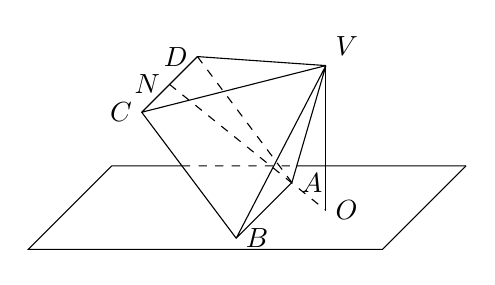
\begin{tikzpicture}
        \coordinate (V) at ({4*sqrt(3)/5},{3*sqrt(3)/5});
        \coordinate (A) at ({3/5+sqrt(2)/4},{-4/5+sqrt(2)/4});
        \coordinate (B) at ({3/5-sqrt(2)/4},{-4/5-sqrt(2)/4});
        \coordinate (C) at ({-3/5-sqrt(2)/4},{4/5-sqrt(2)/4});
        \coordinate (D) at ({-3/5+sqrt(2)/4},{4/5+sqrt(2)/4});
        \draw (V) node [above right] {$V$} -- (A) node [right] {$A$} -- (B) node [right] {$B$} -- (C) node [left] {$C$} -- (D) node [left] {$D$}  (V) -- (B) (V) -- (C) (V) -- (D);
        \draw [dashed] (D) -- (A); 
        \draw (V) -- ({4*sqrt(3)/5},{-4/5}) coordinate (O) node [right] {$O$};
        \draw (B) ++ (225:0.2) ++ (-2.5,0) coordinate (P);
        \draw (P) ++ (4.5,0) coordinate (Q);
        \draw (Q) ++ (45:1.5) coordinate (T) ++ (-4.5,0) coordinate (S);
        \draw (S) -- (P) -- (Q) -- (T);
        \draw ($(C)!0.5!(D)$) node [left] {$N$} coordinate (N);
        \path [name path=A--V] (A) -- (V);
        \path [name path=S--T] (S) -- (T);
        \path [name path=B--C] (B) -- (C);
        \path [name intersections={of = A--V and S--T,by=F}];
        \path [name intersections={of = B--C and S--T,by=E}];
        \draw (S) -- (E) (F) -- (T);
        \draw [dashed] (E) -- (F);
        \draw [dashed] (N) -- (O);
    \end{tikzpicture}
\end{center}
\item {\tiny (003700)}已知$a,b$为空间两条互相垂直的直线, 等腰$\mathrm{Rt}\triangle ABC$的直角边$AC$所在直线与$a,b$都垂直, 斜边$AB$以直线$AC$为旋转轴旋转. 有下列结论: \textcircled{1} 当直线$AB$与$a$所成的角为$60^\circ$时, $AB$与$b$所成的角为$30^\circ$; \textcircled{2} 直线$AB$与$a$所成角的最小值为$45^\circ$; \textcircled{3} 直线$AB$与$a$所成角的最大值为$60^\circ$. 其中所有真命题的序号为\blank{50}.
\item {\tiny (003701)}已知数列$\{a_n\}$满足: \textcircled{1} $a_1=0$; \textcircled{2} 对任意的$n\in \mathbf{N}^*$, 都有$a_{n+1}>a_n$成立. 
函数$f_n(x)=|\sin \dfrac{1}{n}(x-a_n)|, \ x\in [a_n,a_{n+1}]$满足: 对于任意的实数$m\in [0,1)$, $f_n(x)=m$总是有且仅有两个不同的根, 求$\{a_n\}$的通项公式.
\item {\tiny (003702)}设$\overrightarrow a,\overrightarrow b,\overrightarrow c$是平面上的向量,$|\overrightarrow a| =1,|\overrightarrow b| =3,|\overrightarrow c|=4$, 且$\overrightarrow b\cdot \overrightarrow c=0$, 实数$\lambda$满足$0 \le \lambda \le 1$. 若$\overrightarrow a,\overrightarrow b,\overrightarrow c$及$\lambda$, 使得$s=|\overrightarrow a-\lambda \overrightarrow b-(1-\lambda)\overrightarrow c|$是正整数, 则$s$的值的集合是\blank{50}.
\item {\tiny (003703)}如图, 在平面内, $l_1,l_2$是两条平行直线, 它们之间的距离为$2$, 点$P$位于$l_1,l_2$的下方, 它到$l_1$的距离为$1$, 动点$N,M$分别在$l_1,l_2$上, 满足$|\overrightarrow{PM}+\overrightarrow{PN}|=6$, 则$\overrightarrow{PM}\cdot \overrightarrow{PN}$的最大值为\bracket{20}.
\fourch{$6$}{$8$}{$12$}{$15$}
\begin{center}
    \begin{tikzpicture}[>=latex]
        \draw (0,0) -- (5,0) node [right] {$l_1$} (0,2) -- (5,2) node [right] {$l_2$};
        \draw [->] (4.5,-1) node [below right] {$P$} -- (2,0) node [below] {$N$};
        \draw [->] (4.5,-1) -- (2.5,2) node [below] {$M$};
    \end{tikzpicture}
\end{center}
\item {\tiny (003704)}已知过原点$O$的直线与椭圆$C:\dfrac{x^2}4+{y^2}=1$交于$A,B$两点, 点$A$到$y$轴的距离$d$满足$d\in [1,2)$, 点$D$在椭圆$C$上, 且$AD\perp AB$, 直线$BD$与$x$轴、$y$轴分别交于$M,N$两点.\\
(1) 设直线$BD,AM$的斜率分别为$k_1,k_2$, 求$k_1\cdot k_2$的取值范围;\\
(2) 求$\triangle OMN$面积的最大值.
\item {\tiny (003705)}已知点$A(0,\dfrac2n)$, $B(0,-\dfrac2n)$, $C(4+\dfrac2n,0)$, 其中$n$为正整数, 设$S_n$表示$\triangle ABC$外接圆的面积, 则$\displaystyle\lim_{n\to\infty}{S_n}=$\blank{50}.
\item {\tiny (003706)}如图所示: 矩形$A_nB_nP_nQ_n$的一边$A_nB_n$在$x$轴上, 另两个顶点$P_n,Q_n$在函数$f(x)=\dfrac{2x}{1+x^2}$的图像上(其中点$B_n$的坐标为$(n,0) \ (n\ge 2,\ n\in \mathbf{N}^*)$), 矩形$A_nB_nP_nQ_n$的面积记为$S_n$, 则$\displaystyle\lim_{n\to\infty}{S_n}=$\blank{50}.
\begin{center}
    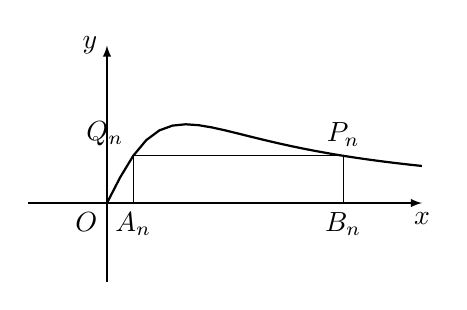
\begin{tikzpicture}[>=latex]
        \draw [->] (-1,0) -- (4,0) node [below] {$x$};
        \draw [->] (0,-1) -- (0,2) node [left] {$y$};
        \draw (0,0) node [below left] {$O$};
        \draw [thick, domain = 0:4] plot (\x,{2*\x/(1+\x*\x)});
        \draw ({1/3},0) node [below] {$A_n$} -- ({1/3},{3/5}) node [above left] {$Q_n$} -- (3,{3/5}) node [above] {$P_n$} -- (3,0) node [below] {$B_n$};
    \end{tikzpicture}
\end{center}
\item {\tiny (003707)}若全集$U=\{x|x^2-7x+12\le 0\}$, 集合$M=\{x|3<x<4\}$, $N=\left\{x\left|\dfrac{x-3}{4-x}\ge 0\right.\right\}$, 则$\complement_U M\cap \complement_U N=$\blank{50}.
\item {\tiny (003708)}设$\alpha:2\le x\le 4$, $\beta: m+1\le x\le 2m+4, \ m\in \mathbf{R}$, 如果$\alpha$是$\beta$的充分非必要条件, 则$m$的范围是\blank{50}.
\item {\tiny (003709)}若函数$y=a^x+b$($a>0$且$a\ne 1$)的图像经过点$(1,7)$, 其反函数的图像经过点$(4,0)$, 则$a-b=$\blank{50}.
\item {\tiny (003710)}已知$\sin\theta=\dfrac 14$, 则$\sin\left[2\left(\theta-\dfrac\pi 4\right)\right]=$\blank{50}.
\item {\tiny (003711)}已知圆锥的母线长为$a$, 轴截面(过轴的截面)为直角三角形, 则圆锥的全面积为\blank{50}.
\item {\tiny (003712)}函数$f(x)=2+\sin x-\tan 2x$, 如果$f(a)=1$, 则$f(-a)=$\blank{50}.
\item {\tiny (003713)}设$S_n$是等差数列$\{a_n\}$的前$n$项和. 若$\dfrac{S_3}{S_7}=\dfrac 13$, 则$\dfrac{S_6}{S_7}=$\blank{50}.
\item {\tiny (003714)}若关于$x$的不等式$|x-3|-|x+2|>a$恒成立, 则实数$a$的范围是\blank{50}.
\item {\tiny (003715)}若$S_n=\dfrac 15+\dfrac {2}{5^2}+\dfrac {1}{5^3}+\dfrac{2}{5^4}+\cdots+\dfrac{1}{5^{2n-1}}+\dfrac{2}{5^{2n}}$, 则$\displaystyle\lim_{n\to \infty}S_n=$\blank{50}.
\item {\tiny (003716)}若函数$f(x)=ax^2+bx+c\ (a>0)$, 不等式$ax^2+bx+c<0$的解集为$\{x|-2<x<0\}$, 当$0<n<m$时, $f(n),f(m),f(\sqrt{mn}),f\left(\dfrac{m+n}2\right)$这四个值中最大的一个是\blank{50}.
\item {\tiny (003717)}设地球半径为$R$, 甲地位于北纬$45^\circ$东经$105^\circ$, 乙地位于南纬$30^\circ$东经$105^\circ$, 则甲乙两地间的球面距离是\blank{30}.
\fourch{$\dfrac{5\pi}{12}R$}{$\dfrac{7\pi}{12}R$}{$\dfrac{\sqrt{2}}2R$}{$\dfrac{\sqrt{3}}2R$}
\item {\tiny (003718)}已知函数$f(x)=\begin{cases}
\log_2(x+4), & x\ge 0,\\f(x+1)-f(x+2), & x<0,\end{cases}$ 则$f(-3)$的值为\blank{30}.
\fourch{$1$}{$0$}{$2$}{$-2$}
\item {\tiny (003719)}若集合$A=\{x|x^2-2x<0\}$, $B=\{x||x|<1\}$, 则$A\cup B$等于\blank{50}.
\item {\tiny (003720)}函数$y=\sqrt{2016^{1-x}}$的定义域是\blank{50}.
\item {\tiny (003721)}已知函数$f(x)=\begin{vmatrix}
1&1\\1&\log_2 x
\end{vmatrix}$, 则$f^{-1}(1)=$\blank{50}.
\item {\tiny (003722)}若复数$\dfrac{1+\mathrm{i}}{1-\mathrm{i}}+\dfrac 12 b \ (b\in \mathbf{R})$的实部的绝对值与虚部相等, 则$b$的值为\blank{50}.
\item {\tiny (003723)}已知$p$为常数, $a_n=\begin{cases}
\dfrac{2n-1}{n+1}, &1\le n\le 2016,\\\left(1+\dfrac 1n\right)^p, & n>2016,
\end{cases}$ 则$\displaystyle\lim_{n\to \infty}a_n=$\blank{50}.
\item {\tiny (003724)}若一个圆锥的母线与轴的夹角为$\arcsin\dfrac 13$, 则该圆锥的侧面积是底面积的\blank{50}倍.
\item {\tiny (003725)}设$x\in\mathbf{R}$, 向量$\overrightarrow{a}=(x,1)$, $\overrightarrow{b}=(1,2)$, 且$\overrightarrow{a}\perp \overrightarrow{b}$, 则$|\overrightarrow{a}+\overrightarrow{b}|=$\blank{50}.
\item {\tiny (003726)}若函数$f(x)=\dfrac{k-2^x}{1+k\cdot 2^x}, \ (k\ne 1, \ k\in \mathbf{R})$在定义域内为奇函数, 则$k=$\blank{50}.
\item {\tiny (003727)}从集合$\{0,1,2,3\}$的所有非空子集中, 等可能地取出一个. 则取出的非空子集中所有元素之和恰为$5$的概率为\blank{50}.
\item {\tiny (003728)}(理科)若对于任意的实数$x\in \mathbf{R}$, 不等式$2x^2-a\sqrt{1+x^2}+3\ge 0$恒成立, 则实数$a$的取值范围为\blank{50}.
\item {\tiny (003729)}``$(2x+1)x=0$''是``$x=0$''的\blank{30}.
\twoch{充分不必要条件}{必要不充分条件}{充分必要条件}{既不充分也不必要条件}
\item {\tiny (003730)}下列函数中, 与函数$y=x^{2n+1} \ (n\in \mathbf{N}^*)$的值域相同的函数为\blank{30}.
\fourch{$y=\left(\dfrac 12\right)^{x+1}$}{$y=\ln(x+1)$}{$y=\dfrac{x+1}{x}$}{$y=x+\dfrac 1x$}
\item {\tiny (003731)}函数$f(x)=x\cos 2x$在区间$[0,2\pi]$上的零点的个数为\blank{30}.
\fourch{$2$}{$3$}{$4$}{$5$}
\item {\tiny (003732)}函数$f(x)=\sqrt{27-3^{2x+1}}$的定义域是\blank{50}.(用区间表示)
\item {\tiny (003733)}已知椭圆中心在原点, 一个焦点为$F(-2\sqrt{3},0)$, 且长轴长是短轴长的$2$倍, 则该椭圆的标准方程是\blank{50}.
\item {\tiny (003734)}实践中常采用``捉--放--捉''的方法估计一个鱼塘中鱼的数量. 如从这个鱼塘中随机捕捞出$100$条鱼, 将这$100$条鱼分别作一记号后再放回鱼塘, 数天后再从鱼塘中随机捕捞出$108$条鱼, 其中有记号的鱼有$9$条, 从而可以估计出鱼塘中的鱼约有\blank{50}条.
\item {\tiny (003735)}若二项式$\left(ax-\dfrac{\sqrt{3}}{6}\right)^3$的展开式的第二项系数为$-\dfrac{\sqrt{3}}{2}$, 则实数$a$的值为\blank{50}.
\item {\tiny (003736)}在$\triangle ABC$中, 角$A,B,C$的对边分别为$a,b,c$. 若$b=\sqrt{5}$, $\angle B=\dfrac{\pi}{4}$, $\tan A=2$, 则$a$等于\blank{50}.
\item {\tiny (003737)}已知数列$\{a_n\}$满足$a_1=a_2=1$, $\dfrac{a_{n+2}}{a_{n+1}}-\dfrac{a_{n+1}}{a_n}=1$, 则$a_6-a_5$的值为\blank{50}.
\item {\tiny (003738)}直线$x=0$, $y=0$与曲线$y=\sqrt{4-x^2}$所围成的图形绕$x$轴旋转一周而成的旋转体的体积等于\blank{50}.
\item {\tiny (003739)}点$P$在双曲线$\dfrac{x^2}{a^2}-\dfrac{y^2}{b^2}=1 \ (a>0, \ b>0)$上, $F_1,F_2$是该双曲线的两个焦点, $\angle F_1PF_2=90^\circ$, 且$\triangle F_1PF_2$的三条边长成等差数列, 则$a:b=$\blank{50}.
\item {\tiny (003740)}(理科)直角坐标系$xOy$中, 以原点为极点, $x$轴的正半轴为极轴建立极坐标系, 已知曲线$C_1: \begin{cases}x=2+2\cos\theta, \\y=2\sin \theta,\end{cases}$($\theta$为参数) 曲线$C_2:\rho\cos\left(\theta+\dfrac{\pi}{3}\right)=t$, 若两曲线有公共点, 则实数$t$的取值范围是\blank{50}.
\item {\tiny (003741)}已知$a>b$, 二次三项式$ax^2+2x+b\ge 0$对于一切实数$x$恒成立. 又存在$x_0\in \mathbf{R}$, 使得$ax_0^2+2x_0+b=0$成立, 则$\dfrac{a^2+b^2}{a-b}$的最小值为\blank{50}.
\item {\tiny (003742)}若$a,b,c\in \mathbf{R}$, 且$a>b$, 则下列不等式一定成立的是\blank{30}.
\fourch{$a+c\ge b-c$}{$ac>bc$}{$\dfrac{c^2}{a-b}>0$}{$(a-b)c^2\ge 0$}
\item {\tiny (003743)}设数列$\{a_n\}$, 下列正确的是\blank{30}.
\onech{若$a_n^2=4^n, \ n\in \mathbf{N}$, 则$\{a_n\}$为等比数列}
{若$a_n\cdot a_{n+2}=a_{n+1}^2, \ n\in\mathbf{N}^*$, 则$\{a_n\}$为等比数列}
{若$a_m\cdot a_n=2^{m+n}, \ m,n\in \mathbf{N}$, 则$\{a_n\}$为等比数列}
{若$a_n\cdot a_{n+3}=a_{n+1}\cdot a_{n+2}, \ n\in \mathbf{N}$, 则$\{a_n\}$为等比数列}
\item {\tiny (003744)}我们规定``渐近线''的概念: 已知曲线$C$, 如果存在有一条直线, 当曲线$C$上任一点$M$沿曲线运动时$M$可无限趋近于该直线但永远达不到, 那么这条直线称为这条曲线的``渐近线''. 下列函数
\textcircled{1} $f(x)=x^2+2x-3$, \textcircled{2} $g(x)=2^x+1$, \textcircled{3} $h(x)=\log_2(x-1)$, \textcircled{4} $t(x)=\dfrac{2x+1}{x-1}$, \textcircled{5} $u(x)=\dfrac{x^2+2}{x}$, 其中有``渐近线''的个数为\blank{30}.
\fourch{$2$}{$3$}{$4$}{$5$}
\item {\tiny (003745)}已知集合$A=\{y|y=\sin x, \ x\in \mathbf{R}\}$, $B=\{x|x(2-x)>0\}$, 则$A\cup B=$\blank{50}.
\item {\tiny (003746)}幂函数$f(x)$的图像经过点$(2,\sqrt{2})$, 且$f^{-1}(x)$为$f(x)$的反函数, 则$f^{-1}(4)=$\blank{50}.
\item {\tiny (003747)}若$\log_a \dfrac 23<1 \ (a>0, \ a\ne 1)$, 则实数$a$的取值范围为\blank{50}.
\item {\tiny (003748)}(理科)设曲线$C$定义为到点$(-1,-1)$和$(1,1)$距离之和为$4$的动点的轨迹. 若将曲线$C$绕坐标原点逆时针旋转$45^\circ$, 则此时曲线$C$的方程为\blank{50}.\\
(文科)椭圆$2x^2+3y^2=6$的焦距为\blank{50}.
\item {\tiny (003749)}已知无穷等比数列$\{a_n\}$的各项和为$4$, 则首项$a_1$的取值范围为\blank{50}.
\item {\tiny (003750)}已知$\left(\sqrt{x}+\dfrac 3{\sqrt[3]{x}}\right)^n$展开式中, 各项系数的和与各项二项式系数的和之差为$56$, 则$n=$\blank{50}.
\item {\tiny (003751)}(理科)设口袋中有黑球、白球共$7$个, 从中任取$2$个球, 已知取到的白球的个数的数学期望为$\dfrac 6 7$, 则口袋中白球的个数为\blank{50}.\\
(文科)从$0,1,2,3,4$这五个数中随机取$2$个数组成一个二位数, 则这个二位数为偶数的概率是\blank{50}.
\item {\tiny (003752)}一个正三棱锥的四个顶点都在半径为$1$的球面上, 其中底面的三个顶点在该球的一个大圆上, 则该正三棱锥的体积是\blank{50}.
\item {\tiny (003753)}将边长为$1$米的正三角形薄片, 沿一条平行于底边的直线剪成两块, 其中一块是梯形, 记$S=\dfrac{(\text{梯形的周长})^2}{\text{梯形的面积}}$, 则$S$的最小值是\blank{50}.
\item {\tiny (003754)}定义区间$(c,d),(c,d],[c,d),[c,d]$的长度均为$d-c\ (d>c)$. 若$a\ne 0$, 关于$x$的不等式$x^2-\left(2a+\dfrac 1a\right)x-1<0$的非空解集(用区间表示)记为$I(a)$, 则当区间$I(a)$的长度取得最小值时, 实数$a$的值为\blank{50}.
\item {\tiny (003755)}过点$(1,0)$且与直线$x-2y-2=0$的法向量垂直的直线方程是\blank{30}.
\twoch{$x-2y+1=0$}{$2x+y-2=0$}{$x+2y-1=0$}{$x-2y-1=0$}
\item {\tiny (003756)}(理科)在极坐标中, 与点$\left(2,\dfrac{\pi}{3}\right)$关于极点对称的点的一个极坐标是\blank{30}.
\fourch{$\left(-2,-\dfrac{\pi}{3}\right)$}{$\left(2,-\dfrac{\pi}{3}\right)$}{$\left(2,-\dfrac{2\pi}{3}\right)$}{$\left(-2,\dfrac{4\pi}{3}\right)$}\\
(文科)如果实数$x,y$满足条件$\begin{cases}
x-y+1\ge 0,\\y+1\ge 0,\\x+y+1\le 0,
\end{cases}$ 那么$2x-y$的最大值为\blank{30}.
\fourch{$2$}{$1$}{$-2$}{$-3$}
\item {\tiny (003757)}设函数$f(x)=x^3+\dfrac{2^x-1}{2^x+1}$, 已知$a\in (-1,1)$, $b\in (-1,1)$. 则$a+b\ge 0$是$f(a)+f(b)\ge 0$的\blank{30}.
\twoch{充分不必要条件}{必要不充分条件}{充分必要条件}{既不充分也不必要条件}
\item {\tiny (003758)}已知$a\in\mathbf{R}$, 命题$P:$``实系数一元二次方程$x^2+ax+2=0$的两根都是虚数''; 命题$Q:$``存在复数$z$同时满足$|z|=2$且$|z+a|=1$''.
是判断命题$P$和命题$Q$之间是否存在推出关系? 说明你的理由.
\item {\tiny (003759)}已知公差不为$0$的等差数列$\{a_n\}$的首项$a_1$为$a \ (a\in \mathbf{R})$, 设数列的前$n$项和为$S_n$, 且$\dfrac{1}{a_1},\dfrac{1}{a_2},\dfrac{1}{a_4}$成等比数列.\\
(1) 求数列$\{a_n\}$的通项公式及$S_n$;\\
(2) 记$A_n=\dfrac{1}{S_1}+\dfrac{1}{S_2}+\dfrac{1}{S_3}+\cdots+\dfrac{1}{S_n}$, $B_n=\dfrac{1}{a_1}+\dfrac{1}{a_2}+\dfrac{1}{a_{2^2}}+\cdots+\dfrac{1}{a_{2^{n-1}}}$, 当$n\ge 2$时, 试比较$A_n$和$B_n$的大小.
\item {\tiny (003760)}已知集合$A=\{1,3,\sqrt{m}\}$, $B=\{1,m\}$, $A\cup B=A$, 则$m=$\blank{50}.
\item {\tiny (003761)}若$\begin{vmatrix}
x^2 & y^2\\-1 & 1
\end{vmatrix}=\begin{vmatrix}
x & x \\ y & -y
\end{vmatrix}$, 则$x+y=$\blank{50}.
\item {\tiny (003762)}若$\dfrac{3+b\mathrm{i}}{a+b\mathrm{i}}=1-\mathrm{i}$($a,b$为实数, $\mathrm{i}$为虚数单位), 则$a+b=$\blank{50}.
\item {\tiny (003763)}已知递增的等差数列$\{a_n\}$满足$a_1=1$, $a_3=a_2^2-4$, 则$a_n=$\blank{50}.
\item {\tiny (003764)}设常数$a\in \mathbf{R}$, 若$\left(x^2+\dfrac ax\right)^5$的二项展开式中$x^7$的系数为$-10$, 则$a=$\blank{50}.
\item {\tiny (003765)}已知双曲线$C_1: \dfrac{x^2}{a^2}-\dfrac{y^2}{b^2}=1 \ (a>0,\ b>0)$与双曲线$C_2: \dfrac{x^2}{4}-\dfrac{y^2}{16}=1$有相同的渐近线, 且$C_1$的右焦点为$F(\sqrt{5},0)$, 则$a=$\blank{50}, $b=$\blank{50}.
\item {\tiny (003766)}(理科)如图, 在极坐标系中, 过点$M(2,0)$的直线$l$与极轴的夹角$\alpha=\dfrac{\pi}{6}$, 若将$l$的极坐标方程写成$\rho=f(\theta)$的形式, 则$f(\theta)=$\blank{50}.
\begin{center}
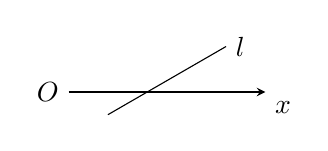
\begin{tikzpicture}[>=stealth]
\draw [->](0,0) node [left] {$O$}--(2.5,0) node [below right]{$x$};
\draw (0.5,{-0.5/sqrt(3)})--(2,{1/sqrt(3)}) node [right] {$l$};
\end{tikzpicture}
\end{center}
\item {\tiny (003767)}某学校组织学生参加英语测试, 成绩的频率分布直方图如图, 数据的分组依次为$[20,40),[40,60),[60,80),[80,100)$. 若低于$60$分的人数是$15$人, 则该班的学生人数是\blank{50}.
\begin{center}
	\begin{tikzpicture}[>=stealth]
	\draw [->](-0.5,0)--(0,0) node [below left] {$O$}--(3,0) node [below right]{成绩$/$分};
	\draw [->] (0,-0.5)--(0,2) node [left] {$\dfrac{\text{频率}}{\text{组距}}$};
	\draw (0.5,0)--(0.5,0.3)--(1,0.3) (1,0)--(1,0.6)--(1.5,0.6) (1.5,0)--(1.5,1.2)--(2,1.2)--(2,0) (2,0.9)--(2.5,0.9)--(2.5,0);
	\draw (0,0.3) node [left] {$0.005$};
	\draw (0,0.6) node [left] {$0.01$};
	\draw (0,0.9) node [left] {$0.015$};
	\draw (0,1.2) node [left] {$0.02$};
	\draw (0.5,0) node [below] {$20$};
	\draw (1,0) node [below] {$40$};
	\draw (1.5,0) node [below] {$60$};
	\draw (2,0) node [below] {$80$};
	\draw (2.5,0) node [below] {$100$};
	\draw [dashed] (0,0.3)--(0.5,0.3) (0,0.6)--(1,0.6) (0,0.9)--(2,0.9) (0,1.2)--(1.5,1.2);
	\end{tikzpicture}
\end{center}
\item {\tiny (003768)}(理科)已知正四棱柱$ABCD-A_1B_1C_1D_1$中, $AA_1=2AB$, 则$CD$与平面$BDC_1$所成角的正弦值等于\blank{50}.
\item {\tiny (003769)}$f(x)$是定义在$\mathbf{R}$上且周期为$2$的函数, 在区间$[-1,1]$上, $f(x)=\begin{cases}ax+1, & -1\le x<0,\\\dfrac{bx+2}{x+1}, & 0\le x\le 1,\end{cases}$ 其中$a,b\in \mathbf{R}$. 若$f\left(\dfrac 12\right)=f\left(\dfrac 32\right)$, 则$a+3b$的值为\blank{50}.
\item {\tiny (003770)}函数$f(x)=2^x+x^3-2$在区间$(0,1)$内的零点的个数是\blank{30}.
\fourch{$0$}{$1$}{$2$}{$3$}
\item {\tiny (003771)}设$\overrightarrow{a},\overrightarrow{b}$都是非零向量, 下列四个条件中, 使$\dfrac{\overrightarrow{a}}{|\overrightarrow{a}|}=\dfrac{\overrightarrow{b}}{|\overrightarrow{b}|}$成立的充分条件是\blank{30}.
\twoch{$|\overrightarrow{a}|=|\overrightarrow{b}|$且$\overrightarrow{a}\parallel \overrightarrow{b}$}{$\overrightarrow{a}=-\overrightarrow{b}$}{$\overrightarrow{a}\parallel\overrightarrow{b}$}{$\overrightarrow{a}=2\overrightarrow{b}$}
\item {\tiny (003772)}定义在$(-\infty,0)\cup (0,+\infty)$上的函数$f(x)$, 如果对于任意给定的等比数列$\{a_n\}$, $\{f(a_n)\}$仍是等比数列, 则称$f(x)$为``保等比数列函数''. 现有定义在$(-\infty,0)\cup (0,+\infty)$上的如下函数: \textcircled{1} $f(x)=x^2$; \textcircled{2} $f(x)=2^x$; \textcircled{3} $f(x)=\sqrt{|x|}$; \textcircled{4} $f(x)=\ln|x|$. 则其中是``保等比数列函数''的$f(x)$的序号为\blank{30}.
\fourch{\textcircled{1}\textcircled{2}}{\textcircled{3}\textcircled{4}}{\textcircled{1}\textcircled{3}}{\textcircled{2}\textcircled{4}}
\item {\tiny (003773)}在锐角$\triangle ABC$中, $a,b,c$分别为内角$A,B,C$所对的边, 且满足$\sqrt{3}a-2b\sin A=0$.\\
(1) 求角$B$的大小;\\
(2) 若$a+c=5$, 且$a>c$, $b=\sqrt{7}$, 求$\triangle ABC$的面积.
\item {\tiny (003774)}已知集合$A=\left\{x\left|\dfrac{2x+1}{x+2}<1, \ x\in \mathbf{R}\right.\right\}$, 函数$f(x)=|mx+1| \ (m\in \mathbf{R})$. 函数$g(x)=x^2+ax+b \ (a,b\in \mathbf{R})$的值域为$[0,+\infty)$.\\
(1) 若不等式$f(x)<3$的解集为$A$, 求$m$的值;\\
(2) 在(1)的条件下, 若$\left|f(x)-2f\left(\dfrac x 2\right)\right|\le k$恒成立, 求$k$的取值范围;\\
(3) 若关于$x$的不等式$g(x)<c$的解集为$(m,m+6)$, 求实数$c$的值.
\item {\tiny (003775)}已知$U=\left\{y\left|y=\log_\frac 12 x, \ x\ge \dfrac 18\right.\right\}$, $A=\left\{x\left|y=\dfrac{1}{\sqrt{2-x}}\right.\right\}$, 则$\complement_U A=$\blank{50}.
\item {\tiny (003776)}命题``已知$x,y\in \mathbf{R}$,  若$x+y>2$, 则$x>1$且$y>1$''的否命题是\blank{150}; 该否命题是\blank{50}命题(填``真'',``假'').
\item {\tiny (003777)}若存在实数$a$, 使得关于$x$的不等式$ax+b>x+1$的解集为$\{x|x<1\}$, 则实数$b$的取值范围为\blank{50}.
\item {\tiny (003778)}已知函数$f(x)=4^x-k\cdot 2^{x+1}+4$在$[0,2]$上存在零点, 则实数$k\in$\blank{50}.
\item {\tiny (003779)}若在$\triangle ABC$中, $2\sin^2A-3\cos A=0$, 则角$A$的大小为\blank{50}.
\item {\tiny (003780)}(理科)在极坐标系中, 若过点$(3,0)$且与极轴垂直的直线交曲线$\rho=4\cos\theta$于$A,B$两点, 则$|AB|=$\blank{50}.
\item {\tiny (003781)}已知直线$l_1:4x-3y+6=0$和直线$l_2:x+1=0$, 抛物线$y^2=4x$上的动点$P$到直线$l_1$和$l_2$的距离之和的最小值为\blank{50}.
\item {\tiny (003782)}若等比数列$\{a_n\}$中$a_2=1$, 则其前$3$项的和$S_3$的取值范围为\blank{50}.
\item {\tiny (003783)}(理科)已知$f(x)$是$\mathbf{R}$上的奇函数, $g(x)$是$\mathbf{R}$上的偶函数, 若函数$f(x)+g(x)$的值域为$[1,3)$, 则$f(x)-g(x)$的值域为\blank{50}.\\
(文科)已知$f(x)$是$\mathbf{R}$上的奇函数, $g(x)$是$\mathbf{R}$上的偶函数, 若函数$f(x)+g(x)$的值域为$[1,3)$, 则$f(-x)+g(x)$的值域为\blank{50}.
\item {\tiny (003784)}给定两个长度为$1$的平面向量$\overrightarrow{OA}$和$\overrightarrow{OB}$, 它们的夹角为$120^\circ$. 如图所示, 点$C$在以$O$为圆心的圆弧$AB$上变动. 若$\overrightarrow{OC}=x\overrightarrow{OA}+y\overrightarrow{OB}$, 其中$x,y\in \mathbf{R}$, 则$x+y$的最大值是\blank{50}.
\begin{center}
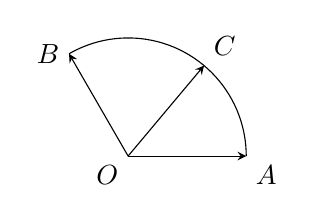
\begin{tikzpicture}[>=stealth]
\draw [->] (0,0) node [below left] {$O$}--(1.5,0) node [below right] {$A$};
\draw [->] (0,0)--({-1.5/2},{0.75*sqrt(3)}) node [left]{$B$};
\draw (1.5,0) arc (0:120:1.5);
\draw [->] (0,0)--({1.5*cos(50)},{1.5*sin(50)}) node [above right] {$C$};
\end{tikzpicture}
\end{center}
\item {\tiny (003785)}已知函数$f(x)=2\sin\left(\dfrac x2+\dfrac \pi 3\right)$, 若对任意的$x\in \mathbf{R}$都有$f(x_1)\le f(x)\le f(x_2)$, 则$|x_1-x_2|$的最小值为\blank{30}.
\fourch{$\dfrac \pi 3$}{$\dfrac{2\pi}{3}$}{$2\pi$}{$4\pi$}
\item {\tiny (003786)}若数列$\{b_n\}$为等比数列, 其前$n$项的和为$S_n$, 若对任意$n\in \mathbf{N}^*$, 点$(n,S_n)$均在函数$y=bx+r$($b>0, \ b\ne 1, \ b,r$为常数)的图像上, 则$r=$\blank{30}.
\fourch{$0$}{$-1$}{$1$}{$2$}
\item {\tiny (003787)}``顺数''是指在一个整数中, 每一位数字比其左边的一位数字大(除首位数字外), 如$24567$就是一个五位``顺数''. 任取一个两位``顺数'', 该数大于$56$的概率为\blank{30}.
\fourch{$\dfrac 13$}{$\dfrac 14$}{$\dfrac {7}{12}$}{$\dfrac{5}{16}$}
\item {\tiny (003788)}如图: 直三棱柱$ABC-A'B'C'$内接于高为$\sqrt{2}$的圆柱中, 已知$\angle ACB=90^\circ$, $AA'=\sqrt{2}$, $BC=AC=1$, $O$为$AB$的中点. \\
(1) 求圆柱的全面积;\\
(2) (文科)求异面直线$AB'$与$CO$所成的角的大小.\\
(理科)求二面角$A'-BC-A$的大小.
\begin{center}
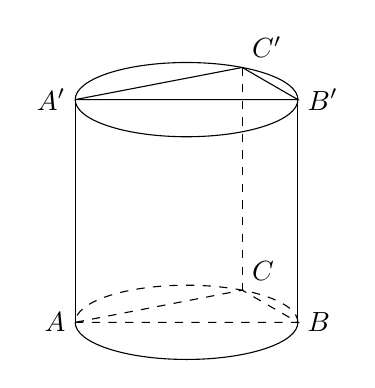
\begin{tikzpicture}
\draw [dashed] (0,0) arc (0:180:{sqrt(2)} and {sqrt(2)/3});
\draw (0,0) arc (0:-180:{sqrt(2)} and {sqrt(2)/3});
\draw (0,{2*sqrt(2)}) arc (0:180:{sqrt(2)} and {sqrt(2)/3});
\draw (0,{2*sqrt(2)}) arc (0:-180:{sqrt(2)} and {sqrt(2)/3});
\draw (0,0)--(0,{2*sqrt(2)}) ({-2*sqrt(2)},0)--({-2*sqrt(2)},{2*sqrt(2)});
\draw [dashed] ({-2*sqrt(2)},0)node [left] {$A$}--(0,0) node [right] {$B$}--({-sqrt(2)+sqrt(2)*cos(60)},{sqrt(2)/3*sin(60)}) node [above right] {$C$}--cycle;
\draw  ({-2*sqrt(2)},{2*sqrt(2)}) node [left] {$A'$}--(0,{2*sqrt(2)}) node [right] {$B'$}--({-sqrt(2)+sqrt(2)*cos(60)},{sqrt(2)/3*sin(60)+2*sqrt(2)}) node [above right] {$C'$}--cycle;
\draw [dashed] ({-sqrt(2)+sqrt(2)*cos(60)},{sqrt(2)/3*sin(60)+2*sqrt(2)})--({-sqrt(2)+sqrt(2)*cos(60)},{sqrt(2)/3*sin(60)});
\end{tikzpicture}
\end{center}
\item {\tiny (003789)}设函数$f(x)=\log_\frac 12 x$, $g(x)=f^{-1}(|x|)$.\\
(1) 求函数$g(x)$的解析式, 并画出大致图像;\\
(2) 若不等式$g(x)+g(2x)\le k$对任意$x\in \mathbf{R}$恒成立, 求实数$k$的取值范围.
\item {\tiny (003790)}已知$f(x)=1-x^2 \ (x<-1)$, 则$f^{-1}(-3)=$\blank{50}.
\item {\tiny (003791)}已知$\alpha\in \left(\dfrac{\pi}{2},\pi\right)$, $\sin\alpha=\dfrac{3}{5}$, 则$\tan\left(\alpha+\dfrac{\pi}{4}\right)=$\blank{50}.
\item {\tiny (003792)}若关于$x,y$的二元线性方程组的增广矩阵为$\begin{pmatrix}1 & 3 & 5\\2 & 4 & 6\end{pmatrix}$, 则$x-y=$\blank{50}.
\item {\tiny (003793)}已知某圆锥的体积是$12\pi$cm$^2$, 底面半径等于$3$cm, 则该圆锥的高为\blank{50}.
\item {\tiny (003794)}若复数$z=\left(\dfrac 12-\dfrac{\sqrt{3}}{2}\mathrm{i}\right)^2$是实系数方程$ax^2+bx+1=0$的根, 则$a\cdot b=$\blank{50}.
\item {\tiny (003795)}某抛物线形拱桥的跨度为$20$米, 拱高是$4$米, 在建桥时, 每隔$4$米需用一根支柱支撑, 其中最高支柱的高度是\blank{50}米.(答案保留两位小数)
\item {\tiny (003796)}(理科)化极坐标方程$(\rho-2)\left(\theta-\dfrac{\pi}{3}\right)=0$为直角坐标方程: \blank{100}.
\item {\tiny (003797)}设$x,y$均为正实数, 且$\dfrac{1}{2+x}+\dfrac{1}{2+y}=\dfrac 14$, 则$xy$的最小值为\blank{50}.
\item {\tiny (003798)}三角形的三内角$A,B,C$所对边的长分别为$a,b,c$, 设向量$\overrightarrow{m}=(a-b,a-c)$, $\overrightarrow{n}=(c,a+b)$. 若$\overrightarrow{m}\parallel \overrightarrow{n}$, 则角$B$的大小为\blank{50}.
\item {\tiny (003799)}已知$f(x)=4-\dfrac 1x$, 若存在区间$[a,b]\subseteq \left(\dfrac 13,+\infty\right)$, 使得$\{y|y=f(x), \ x\in [a,b]\}=[ma,mb]$, 则实数$m$的取值范围是\blank{50}.
\item {\tiny (003800)}下列命题中正确的是\blank{30}.
\twoch{若$ac>bc$, 则$a>b$}{若$a^2>b^2$, 则$a>b$}{若$\dfrac 1a>\dfrac 1b$, 则$a<b$}{若$\sqrt{a}<\sqrt{b}$, 则$a<b$}
\item {\tiny (003801)}下列函数中, 既是偶函数, 又是在区间$(0,+\infty)$上单调递减的函数为\blank{30}.
\fourch{$y=\lg\dfrac{1}{|x|}$}{$y=x^3$}{$y=3^{|x|}$}{$y=x^2$}
\item {\tiny (003802)}已知数列$\{a_n\}$是等差数列, 则``$a_1+a_9<a_4+a_7$''是``$\{a_n\}$为递增数列''的\blank{30}.
\twoch{充分非必要条件}{必要非充分条件}{充要条件}{既非充分又非必要条件}
\item {\tiny (003803)}某校高一年级开设研究性学习课程, 一班和二班报名参加的人数分别是$18$和$27$. 现用分层抽样的方法, 从中抽取若干名学生组成研究性学习小组, 已知从二班抽取了$3$名同学.\\
(1) 求研究性学习小组的人数;\\
(2) 规划在研究性学习的中、后期各安排$1$次交流活动, 每次随机抽取小组中$1$名同学发言. 求$2$次发言的学生恰好来自不同班级的概率.
\item {\tiny (003804)}已知点$A(-1,0)$, $B(1,0)$, $C\left(-\dfrac{5\sqrt{7}}{12},0\right)$, $D\left(\dfrac{5\sqrt{7}}{12},0\right)$, 动点$P(x,y)$满足$\overrightarrow{AP}\cdot\overrightarrow{BP}=0$, 动点$Q(x,y)$满足$|\overrightarrow{QC}|+|\overrightarrow{QD}|=\dfrac{10}{3}$.\\
(1) 求动点$P$的轨迹方程$C_0$和动点$Q$的轨迹方程$C_1$;\\
(2) 是否存在与曲线$C_0$外切且与曲线$C_1$内接的平行四边形? 若存在, 请求出{\bf 一个}这样的四边形; 若不存在, 说明理由;\\
(3) 固定曲线$C_0$, 在(2)的基础上提出一个一般性的问题, 使(2)成为(3)的特例, 探究能得出相应结论(或加强结论)需满足的条件, 并说明理由.
\item {\tiny (003805)}已知命题$p:$``若$\overrightarrow{a}=\overrightarrow{b}$, 则$|\overrightarrow{a}|=|\overrightarrow{b}|$'', 则命题$p$及其逆命题, 否命题, 逆否命题中, 正确命题的个数是\blank{50}.
\item {\tiny (003806)}在一次教师联欢会上, 到会的女教师比男教师多$12$人, 从到会教师中随机挑选一人表演节目. 如果每位教师被选中的概率相等, 而且选中男教师的概率为$\dfrac 9{20}$, 那么参加这次联欢会的教师共有\blank{50}人.
\item {\tiny (003807)}在$\triangle ABC$中, $C=60^\circ$, $AB=\sqrt{3}$, $BC=\sqrt{2}$, 那么$A=$\blank{50}.
\item {\tiny (003808)}设$A,B,C$是圆$x^2+y^2=1$上不同的三个点, $O$为圆心, 且$\overrightarrow{OA}\cdot\overrightarrow{OB}=0$, 存在实数$\lambda,\mu$使得$\overrightarrow{OC}=\lambda\overrightarrow{OA}+\mu\overrightarrow{OB}$, 则实数$\lambda$和$\mu$的关系为\blank{50}.
\item {\tiny (003809)}如下图所示的程序框图中, 循环体执行的次数是\blank{50}.
\begin{center}
\begin{tikzpicture}[>=stealth]
\draw (0,-0.3)--(1,-0.3) arc (-90:90:0.3)--(0,0.3) arc (90:270:0.3);
\draw (0.5,0) node {开始};
\draw [->] (1.3,0)--(1.6,0);
\draw (1.6,-0.3) rectangle (4,0.3);
\draw (2.8,0) node {$i=2, \ S=0$};
\draw [->] (4,0)--(4.3,0);
\draw (4.3,-0.3) rectangle (6.3,0.3);
\draw (5.3,0) node {$S=S+i$};
\draw [->] (6.3,0)--(6.6,0);
\draw (6.6,-0.3) rectangle (8.6,0.3);
\draw (7.6,0) node {$i=i+2$};
\draw [->] (8.6,0)--(8.9,0);
\draw [->] (8.9,0)--(10,0.5)--(11.1,0)--(10,-0.5)--cycle;
\draw (10,0) node {$i\ge 100$};
\draw [->] (11.1,0) node [above right] {是}--(12,0);
\draw (11.7,-0.3)--(12.3,0.3)--(14.1,0.3)--(13.5,-0.3)--cycle;
\draw (12.9,0) node {输出$S$};
\draw [->] (13.8,0)--(14.1,0);
\draw (14.4,-0.3)--(15.4,-0.3) arc (-90:90:0.3)--(14.4,0.3) arc (90:270:0.3);
\draw (14.9,0) node {结束};
\draw [->] (10,-0.5) node [below right] {否}--(10,-1)--(4.15,-1)--(4.15,0);
\end{tikzpicture}
\end{center}
\item {\tiny (003810)}设常数$a>0$, 若对任意正实数$x,y$, 不等式$(x+y)\cdot\left(\dfrac 1x+\dfrac ay\right)\ge 9$恒成立, 则$a$的最小值为\blank{50}.
\item {\tiny (003811)}若$(1-2x)^{2014}=a_0+a_1x+a_2x^2+\cdots+a_{2014}x^{2014} \ (x\in \mathbf{R})$, 则$\dfrac{a_1}{2}+\dfrac{a_2}{2^2}+\cdots+\dfrac{a_{2014}}{2^{2014}}$的值为\blank{50}.
\item {\tiny (003812)}若三个人踢毽, 互相传递, 每人每次只能踢以下, 由甲开始踢, 经过$5$次传递后, 毽又被踢回给甲, 则不同的传递方式共有\blank{50}种.
\item {\tiny (003813)}在数列$\{a_n\}$中, 若$a_n^2-a_{n+1}^2=p\ (n\ge 1, \ n\in\mathbf{N}^*, \ p$为常数$)$, 则称$\{a_n\}$为``等方差数列''. 下列是对``等方差数列''的判断,
\textcircled{1} 若$\{a_n\}$是等方差数列, 则$\{a_n^2\}$是等差数列;
\textcircled{2} $\{(-1)^n\}$是等方差数列;
\textcircled{3} 若$\{a_n\}$是等方差数列, 则$\{a_{kn}\} \ (k\in \mathbf{N}^*, \ k$为常数$)$也是等方差数列.
其中真命题的序号为\blank{50}(将所有真命题的序号填写在横线上).
\item {\tiny (003814)}(理科)在极坐标系中, 圆$\rho=2\cos\theta$的圆心到直线$\rho\cos\theta=2$的距离是\blank{50}.
\item {\tiny (003815)}在同一坐标系中画出函数$y=\log_a x, \ y=a^x, y=x+a$的图像, 可能正确的是\blank{30}.
\fourch{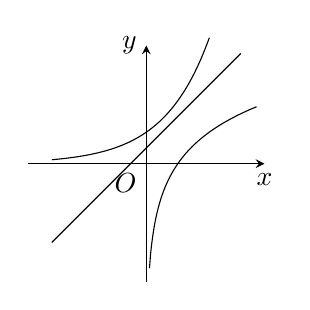
\begin{tikzpicture}[>=stealth,samples=100]
	\draw [->] (-1.5,0)--(0,0) node [below left] {$O$}--(1.5,0) node [below] {$x$};
	\draw [->] (0,-1.5)--(0,1.5) node [left] {$y$};
	\draw [domain=-3:3] plot ({\x*0.4},{(\x+0.5)*0.4});
	\draw [domain=-3:2] plot ({\x*0.4},{exp(\x*ln(2))*0.4});
	\draw [domain=0.1:3.5] plot ({\x*0.4},{ln(\x)/ln(2)*0.4});
	\end{tikzpicture}}{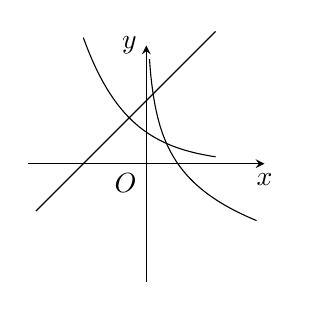
\begin{tikzpicture}[>=stealth,samples=100]
	\draw [->] (-1.5,0)--(0,0) node [below left] {$O$}--(1.5,0) node [below] {$x$};
	\draw [->] (0,-1.5)--(0,1.5) node [left] {$y$};
	\draw [domain=-3.5:2.2] plot ({\x*0.4},{(\x+2)*0.4});
	\draw [domain=-2:2.2] plot ({\x*0.4},{exp(\x*ln(1/2))*0.4});
	\draw [domain=0.1:3.5] plot ({\x*0.4},{-ln(\x)/ln(2)*0.4});
	\end{tikzpicture}}{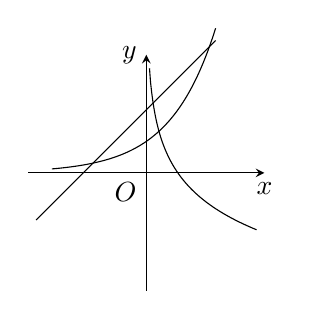
\begin{tikzpicture}[>=stealth,samples=100]
	\draw [->] (-1.5,0)--(0,0) node [below left] {$O$}--(1.5,0) node [below] {$x$};
	\draw [->] (0,-1.5)--(0,1.5) node [left] {$y$};
	\draw [domain=-3.5:2.2] plot ({\x*0.4},{(\x+2)*0.4});
	\draw [domain=-3:2.2] plot ({\x*0.4},{exp(\x*ln(2))*0.4});
	\draw [domain=0.1:3.5] plot ({\x*0.4},{-ln(\x)/ln(2)*0.4});
	\end{tikzpicture}}{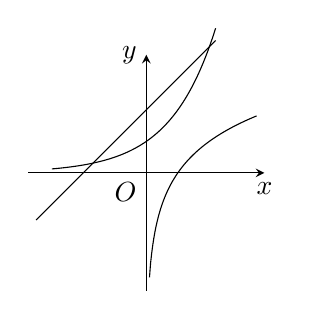
\begin{tikzpicture}[>=stealth,samples=100]
	\draw [->] (-1.5,0)--(0,0) node [below left] {$O$}--(1.5,0) node [below] {$x$};
	\draw [->] (0,-1.5)--(0,1.5) node [left] {$y$};
	\draw [domain=-3.5:2.2] plot ({\x*0.4},{(\x+2)*0.4});
	\draw [domain=-3:2.2] plot ({\x*0.4},{exp(\x*ln(2))*0.4});
	\draw [domain=0.1:3.5] plot ({\x*0.4},{ln(\x)/ln(2)*0.4});
	\end{tikzpicture}}
\item {\tiny (003816)}(理科)如图, 四棱锥$S-ABCD$的底面为正方形, $SD\perp $底面$ABCD$, 则下列结论中{\bf 不正确}的是\blank{30}
\twoch{$AC\perp SB$}{$AB\parallel$平面$SCD$}{$AB$与$SC$所成的角等于$DC$与$SA$所成的角}{$SA$与平面$SBD$所成的角等于$SC$与平面$SBD$所成的角}\\
(文科)如图, 在四面体$A-BCD$中, 截面$PQMN$是正方形, $PQ\parallel AC$, $QM\parallel BD$, 则下列命题中, 正确的有\blank{30}.
\textcircled{1} $AC\perp BD$; \textcircled{2} $AC\parallel$截面$PQMN$; \textcircled{3} $AC=BD$; \textcircled{4} 异面直线$PM$与$BD$所成的角为$45^\circ$.
\fourch{\textcircled{1}\textcircled{2}\textcircled{3}}{\textcircled{1}\textcircled{3}\textcircled{4}}{\textcircled{1}\textcircled{2}\textcircled{4}}{\textcircled{2}\textcircled{3}\textcircled{4}}
\begin{center}
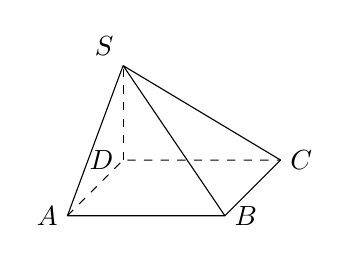
\begin{tikzpicture}
\draw (0,0) node [left] {$A$} coordinate (A)--(2,0) node [right] {$B$} coordinate (B)--({2+0.5*sqrt(2)},{0.5*sqrt(2)}) node [right] {$C$} coordinate (C);
\draw [dashed] (A)--({0.5*sqrt(2)},{0.5*sqrt(2)}) node[left]{$D$} coordinate (D)--(C);
\draw [dashed] (D)--+(0,1.2) node[above left] {$S$} coordinate (S);
\draw (S)--(A) (S)--(B) (S)--(C);
\end{tikzpicture}
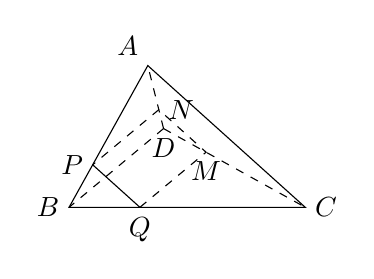
\begin{tikzpicture}
\draw (0,0) coordinate (B) node[left]{$B$}--(3,0) coordinate (C) node [right] {$C$}--(1,1.8) node [above left] {$A$} coordinate (A)--cycle;
\draw [dashed] (1.2,1) node [below]{$D$} coordinate (D)--(A) (D)--(B) (D)--(C);
\coordinate (P) at ($(A)!0.7!(B)$);
\coordinate (Q) at ($(C)!0.7!(B)$);
\coordinate (M) at ($(C)!0.7!(D)$);
\coordinate (N) at ($(A)!0.7!(D)$);
\draw (P) node [left] {$P$}--(Q) node [below] {$Q$};
\draw [dashed] (Q)--(M) node [below] {$M$} --(N) node [right] {$N$} --(P);
\end{tikzpicture}
\end{center}
\newpage
\item {\tiny (003817)}观察下列等式: 
\textcircled{1} $\cos 2\alpha=2\cos^2\alpha-1$; \textcircled{2} $\cos 4\alpha=8\cos^4\alpha-8\cos^2\alpha+1$; \textcircled{3} $\cos 6\alpha=32\cos^6\alpha-48\cos^4\alpha+18\cos^2\alpha-1$; \textcircled{4} $\cos 8\alpha=128\cos^8\alpha-256\cos^6\alpha+160\cos^4\alpha-32\cos^2\alpha+1$ \textcircled{5} $\cos10\alpha=m\cos^{10}\alpha-1280\cos^8\alpha+1120\cos^6\alpha+n\cos^4\alpha+p\cos^2\alpha-1$.
由此可以推测$m-n+p=$\blank{30}.
\fourch{$962$}{$963$}{$964$}{$965$}
\item {\tiny (003818)}已知$P=\{x|x^2-8x-20\le 0\}$, $S=\{x|1-m\le x\le 1+m\}$.\\
(1) 是否存在实数$m$, 使$x\in P$是$x\in S$的充要条件, 若存在, 求出$m$的范围;\\
(2) 是否存在实数$m$, 使$x\in P$是$x\in S$的必要条件, 若存在, 求出$m$的范围.
\item {\tiny (003819)}已知圆$C_1: \left(x+\dfrac{\sqrt{6}}{2}\right)^2+y^2=\dfrac{25}{8}$, 圆$C_2: \left(x-\dfrac{\sqrt{6}}{2}\right)^2+y^2=\dfrac{1}{8}$. 动圆$P$与已知两圆都外切.\\
(1) 求动圆的圆心$P$的轨迹$E$的方程;\\
(2) 直线$l: y=kx+1$与点$P$的轨迹$E$交于不同的两点$A,B$, $AB$的中垂线与$y$轴交于点$N$, 求点$N$的纵坐标的取值范围.
\item {\tiny (003820)}已知向量$\overrightarrow{a}=(1,k)$, $\overrightarrow{b}=(2,2)$, 若$\overrightarrow{a}+\overrightarrow{b}$与$\overrightarrow{a}$共线, 计算$\overrightarrow{a}\cdot\overrightarrow{b}=$\blank{50}.
\item {\tiny (003821)}复数$\dfrac{m+\mathrm{i}}{1+\mathrm{i}}-\dfrac 12$的实部与虚部相等, 则实数$m$的值为\blank{50}.
\item {\tiny (003822)}若$\displaystyle\lim_{n\to \infty}\left(\dfrac{an^2+cn+2}{2n+1}-n\right)=3$, 则$a+c=$\blank{50}.
\item {\tiny (003823)}已知关于$x,y$的二元一次方程组的增广矩阵为$\begin{pmatrix}2 & 3 & 1 \\1 & 1 & 2\end{pmatrix}$, 则$D_x=$\blank{50}.
\item {\tiny (003824)}若$\theta$是某三角形的内角且$\cos2\theta+3\cos\theta+1=0$, 则$\theta=$\blank{50}.
\item {\tiny (003825)}(理科)有$3$位射击手独立瞄准一个相同目标, 他们命中的概率都是$0.8$, 则目标恰好被两名射手命中的概率是\blank{50}.\\
(文科)袋子中有大小形状相同的$4$个红球, $3$个白球, 某人随机抽出两个球, 则恰好是一红一白的概率是\blank{50}.
\item {\tiny (003826)}已知$F_1,F_2$为椭圆$\dfrac{x^2}{25}+\dfrac{y^2}{16}=1$的左、右焦点, $P$为椭圆上一点, $M$是$F_1P$的中点, $|OM|=3$, 则点$M$到椭圆左焦点的距离为\blank{50}.
\item {\tiny (003827)}(理科)正三棱锥$P-ABC$中, 点$P,A,B,C$都在半径为$\sqrt{3}$的球面上, 若$PA,PB,PC$两两互相垂直, 则球心到截面$ABC$的距离为\blank{50}.
\item {\tiny (003828)}已知正数$x,y$满足$\ln x+\ln y=\ln (x+y)$, 则$2x+y$的最小值是\blank{50}.
\item {\tiny (003829)}二维空间中圆的一维测度(周长)$l=2\pi r$, 二维测度(面积)$S=\pi r^2$; 三维空间中球的二维测度(表面积)$S=4\pi r^2$, 三维测度(体积)$V=\dfrac 43\pi r^3$; 类比观察, 则四维空间中``超球''的三维测度$V=8\pi r^3$, 猜想其四维测度$W=$\blank{50}.
\item {\tiny (003830)}设$l,m,n$是直线, 其中$m,n$在平面$\alpha$内, 则``$l\perp \alpha$''是``$l\perp m, \ l\perp n$''的\blank{30}.
\twoch{充分不必要条件}{必要不充分条件}{充要条件}{既不充分也不必要条件}
\item {\tiny (003831)}方程$(2x+3y-1)(\sqrt{x-3}-1)=0$表示的曲线是\blank{30}.
\fourch{两条直线}{两条射线}{两条线段}{一条直线和一条射线}
\item {\tiny (003832)}已知等比数列$\{a_n\}$的公比$q<0$, 其前$n$项和为$S_n$, 则$a_9S_8$与$a_8S_9$的大小关系是\blank{30}.
\twoch{$a_9S_8>a_8S_9$}{$a_9S_8<a_8S_9$}{$a_9S_8\ge a_8S_9$且可能取到等号}{$a_9S_8\le a_8S_9$且可能取到等号}
\item {\tiny (003833)}已知正数$a,b,c,d$满足$ac\ne bd$. 求证: $\dfrac{a+d}{b+c}$在$\dfrac ab$与$\dfrac dc$之间.
\item {\tiny (003834)}已知$\{a_n\}$为无穷等比数列, 数列$\{b_n\}$满足$b_1+b_2+\cdots+b_n=\dfrac{n}{n+1} \ (n\in \mathbf{N}^*)$, 且$a_1+3b_2=2$, $\displaystyle_{n\to \infty}(a_1+a_2+a_3+\cdots+a_n)=\dfrac 56$. \\
(1) 求数列$\{a_n\}$和$\{b_n\}$的通项公式;\\
(2) 是否存在$m\in \mathbf{N}^*$, 使得当正整数$n\ge m$时, 总有$a_n<b_n$? 若有, 求出$m$的最小值; 若没有, 请说明理由.
\item {\tiny (003835)}若集合$A=\{x||x-2|\le 2\}$, $B=\{y|y=-x^2, \ -1\le x\le 2\}$, 则$A\cap B=$\blank{50}.
\item {\tiny (003836)}若$z_1,z_2$是方程$z^4=4$的两个虚根, 则$z_1\cdot z_2=$\blank{50}.
\item {\tiny (003837)}若抛物线$y^2=2mx$的焦点与双曲线$\dfrac{x^2}{2}-\dfrac{y^2}{2}=1$的右焦点重合, 则$m=$\blank{50}.
\item {\tiny (003838)}已知函数$f(x)=\begin{cases}
\dfrac 3x, & x\ge 3,\\ \log_3 x, & 0<x<3,
\end{cases}$ 若关于$x$的方程$f(x)=k$有两个不同的实根, 则实数$k$的取值范围是\blank{50}.
\item {\tiny (003839)}方程$\dfrac{\sin x}{1+\cos x}=\dfrac{1-\cos x}{\sin x}$的解集为\blank{50}.
\item {\tiny (003840)}若$(1+x)^n+\left(1+x^\frac 12\right)^n+\left(1+x^\frac 13\right)^n+\cdots+\left(1+x^\frac 1n\right)^n \ (n\in \mathbf{N}^*)$的展开式中$x$的系数是$a_n$, 展开式中所有项的系数和为$b_n$, 则$\displaystyle\lim_{n\to \infty}\dfrac{na_n}{b_n}=$\blank{50}.
\item {\tiny (003841)}如图, $M$是平行四边形$ABCD$的边$AB$的中点, 直线$l$过点$M$分别交$AD,AC$于点$E,F$. 若$\overrightarrow{AD}=3\overrightarrow{AE}$, 则$AF:FC=$\blank{50}.
\begin{center}
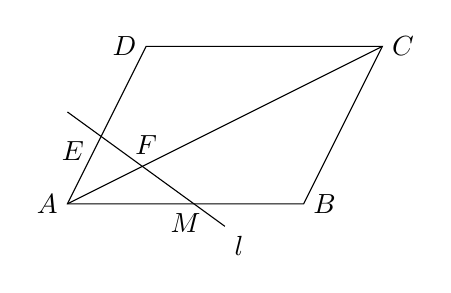
\begin{tikzpicture}
\draw (0,0) node [left] {$A$}--(3,0) node [right] {$B$}--(4,2) node [right] {$C$}--(1,2) node [left] {$D$}--cycle;
\draw (0,0)--(4,2);
\draw (0,{7/6})--(2,{-2/7}) node [below right] {$l$};
\draw ({3/2},0) node [below] {$M$} ({1/3},{2/3}) node [left] {$E$} (1,0.5) node [above] {$F$};
\end{tikzpicture}
\end{center}
\item {\tiny (003842)}(理科)某学生在参加政、史、地三门课程的学业水平考试中, 取得A等级的概率分别为$\dfrac 45$, $\dfrac 35$, $\dfrac 25$, 且三门课程的成绩是否取得A等级相互独立. 记$\xi$为该生取得A等级的课程数, 则数学期望$E\xi$的值为\blank{50}.
\item {\tiny (003843)}已知公比为$q(q>0)$的等比数列$\{a_n\}$中, $a_1=256$, 记$\prod_n=a_1\times a_2\times \cdots\times a_n$(即$\prod _n$表示数列$\{a_n\}$的前$n$项之积), 若$\{\prod_n\}$中最大项有且只有$\prod_9$, 则$q$的取值范围是\blank{50}.
\item {\tiny (003844)}(理科)一质点从所有棱长都为$1$的正五棱柱$ABCDE-A_1B_1C_1D_1E_1$的顶点$E$出发, 沿正五棱柱的棱运动, 每过一条棱称为一次运动. 运动方向是$E\to A\to B\to B_1\to \cdots$, 从开始在$EA$上称为第$1$棱运动, $AB$上称为第$2$棱运动, $BB_1$上称为第$3$棱运动, $\cdots$, 且第$n+2$棱运动所在棱与第$n$棱运动所在棱是异面直线. 经过$2014$次运动后, 质点到达顶点位置时\blank{50}.\\
(文科)质点从正方体$ABCD-A_1B_1C_1D_1$的顶点$A$出发, 沿正方体的棱运动. 每经过一条棱称为一次运动. 第一次从$A$到$B$, 第二次从$B$到$C$, 运动规律满足第$n+2$次运动所在棱与第$n$次运动所在棱成异面直线. 那么质点经$2014$次运动后到达顶点位置为\blank{50}.
\item {\tiny (003845)}为了从甲乙两人中选一人参加数学竞赛,老师将两人最近的$6$次数学测试的分数进行统计, 甲乙两人的得分情况如下表所示, 
\begin{center}
\begin{tabular}{|c|c|c|c|c|c|c|}
	\hline
	甲 & $72$ & $78$ & $79$ & $85$ & $86$ & $92$\\ \hline
	乙 & $78$ & $86$ & $88$ & $88$ & $91$ & $93$\\ \hline
\end{tabular}
\end{center}
若甲乙两人的平均成绩分别是$\bar{x}_{\text{甲}}$, $\bar{x}_{\text{乙}}$, 则下列说法正确的是\blank{30}.
\twoch{$\bar{x}_{\text{甲}}>\bar{x}_{\text{乙}}$, 乙比甲成绩稳定, 应该选乙参加比赛}{$\bar{x}_{\text{甲}}>\bar{x}_{\text{乙}}$, 甲比乙成绩稳定, 应该选甲参加比赛}{$\bar{x}_{\text{甲}}<\bar{x}_{\text{乙}}$, 甲比乙成绩稳定, 应该选甲参加比赛}{$\bar{x}_{\text{甲}}<\bar{x}_{\text{乙}}$, 乙比甲成绩稳定, 应该选乙参加比赛}
\item {\tiny (003846)}已知$m,n$是两条不同直线, $\alpha,\beta,\gamma$是三个不同平面, 下列命题中正确的是\blank{30}.
\twoch{$m\parallel \alpha$, $n\parallel \alpha$, 则$m\parallel n$}{若$m\parallel \alpha$, $m\parallel \beta$, 则$\alpha\parallel \beta$}{若$\alpha\perp \gamma$, $\beta\perp \gamma$, 则$\alpha\parallel \beta$}{若$m\perp \alpha$, $n\perp \alpha$, 则$m\parallel n$}
\item {\tiny (003847)}平面四边形$ABCD$中, $\overrightarrow{AB}+\overrightarrow{CD}=\overrightarrow{0}$, $(\overrightarrow{AB}-\overrightarrow{AD})\cdot \overrightarrow{AC}=0$, 则四边形$ABCD$是\blank{30}.
\fourch{矩形}{菱形}{等腰梯形}{直角梯形}
\item {\tiny (003848)}已知函数$f(x)=x\begin{vmatrix}
\mathrm{e}^{2x} & 1\\-\mathrm{e}^x & a
\end{vmatrix}$, 其中$\mathrm{e}$是自然对数的底数, $a\in \mathbf{R}$.\\
(1) 当$-1<a<0$时, 解不等式$f(x)<0$;\\
(2) 当$a=0$时, 求整数$t$的所有值, 使方程$f(x)=x+2$在$[t,t+1]$上有解.
\item {\tiny (003849)}如图是一个算法的流程图.\\
(1) 写出数列$\{a_n\}$的前$6$项;\\
(2) 试求输出$S$的值.
\begin{center}
\begin{tikzpicture}[>=stealth]
\draw (-0.5,0) arc (270:90:0.3)--(0.5,0.6) arc (90:-90:0.3) --cycle;
\draw (0,0.3) node {开始};
\draw [->] (0,0)--(0,-0.6);
\draw (-1.2,-0.6) rectangle (1.2,-1.2);
\draw (0,-0.9) node {$i=1, \ S=0$};
\draw [->] (0,-1.2)--(0,-1.8);
\draw (-1.5,-1.8) rectangle (1.5,-2.7);
\draw (0,-2.25) node {$a_i=i\cos\dfrac{i\pi}{2}+1$};
\draw [->] (0,-2.7)--(0,-3.3);
\draw (-1.2,-3.3) rectangle (1.2,-3.9);
\draw (0,-3.6) node {$S=S+a_i$};
\draw [->] (0,-3.9)--(0,-4.5);
\draw (0,-4.5)--(-1.2,-5)--(0,-5.5)--(1.2,-5)--cycle;
\draw (0,-5) node {$i<2014$};
\draw [->] (0,-5.5)--(0,-6.1);
\draw (0,-5.8) node [left] {否};
\draw [->] (1.2,-5) node [above right] {是} -- (3.2,-5)--(3.2,-3.9);
\draw (2,-3.9) rectangle (4.4,-3.3);
\draw (3.2,-3.6) node {$i=i+1$};
\draw [->] (3.2,-3.3)--(3.2,-1.5)--(0,-1.5);
\draw (-0.6,-6.1)--(1,-6.1)--(0.6,-6.7)--(-1,-6.7)--cycle (0,-6.4) node {输出$S$};
\draw [->] (0,-6.7)--(0,-7.3);
\draw (-0.5,-7.9) arc (270:90:0.3)--(0.5,-7.3) arc (90:-90:0.3) --cycle;
\draw (0,-7.6) node {结束};
\end{tikzpicture}
\end{center}
\item {\tiny (003850)}设$\dfrac{\sqrt{3}-\tan\left(\dfrac{\pi}{3}-\theta\right)}{1+\sqrt{3}\tan\left(\dfrac{\pi}{3}-\theta\right)}=3$, 则$\cos 2\theta$等于\blank{50}.
\item {\tiny (003851)}在$(1+x)^n$的展开式中, 第十项是使得二项式系数最大的唯一的项, 则$n$的值是\blank{50}.
\item {\tiny (003852)}光线每穿过一块玻璃板, 其强度就要损失$10\%$, 要使光线的强度减弱到原来的$\dfrac 13$以下, 那么至少需要重叠\blank{50}块玻璃板.
\item {\tiny (003853)}若$|\overrightarrow a|=10$, $\overrightarrow b=(3,-4)$, 且$\overrightarrow a$与$\overrightarrow b$的方向相同, 则$\overrightarrow a=$\blank{50}.
\item {\tiny (003854)}不等式$\lg(-x)<x+1$的解集为\blank{50}.
\item {\tiny (003855)}某科技小组有$6$名同学, 现从中选出$3$人去参观展览, 至少有$1$名女生入选时的不同选法有$16$中, 则小组中的女生人数为\blank{50}.
\item {\tiny (003856)}若用边长为$4$的正方形纸片制作一个母线长为$4$的无底圆锥, 则这样制作出的圆锥的最大体积为\blank{50}.
\item {\tiny (003857)}已知$f(x)=\begin{cases}
1, & x\ge 0,\\-1, & x<0,
\end{cases}$ 则不等式$x+(x+2)f(x+2)\le 5$的解集是\blank{50}.
\item {\tiny (003858)}椭圆$\dfrac{x^2}{a^2}+\dfrac{y^2}{b^2}=1 \ (a>b>0)$和圆$x^2+y^2=\left(\dfrac b2+c\right)^2 \ (c^2=a^2-b^2)$有两个不同的公共点, 则$\dfrac ca$的值是\blank{50}.
\item {\tiny (003859)}设数列$\{a_n\}$为$\dfrac 12,\dfrac 13+\dfrac 23,\dfrac 14+\dfrac 24+\dfrac 34,\cdots$, 若$b_n=\dfrac{1}{a_na_{n+1}}$, 记$\{b_n\}$的前$n$项和为$S_n$, 则$S_{11}$的值为\blank{50}.
\item {\tiny (003860)}若集合$M=\{y|y=x^2-1, \ x\in \mathbf{R}\}$, 集合$N=\{x|y=\sqrt{3-x}, \ x\in \mathbf{R}\}$, 则$M\cap N=$\blank{30}.
\fourch{$\{(-\sqrt{2},1),(\sqrt{2},1)\}$}{$\{t|0\le t\le \sqrt{3}\}$}{$\{t|-1\le t\le 3\}$}{$\{t|-\infty<t\le \sqrt{3}\}$}
\item {\tiny (003861)}设$A(-1,0)$, $B(1,0)$, 条件甲: $A,B,C$是以$C$为直角顶点的三角形的三个顶点; 条件乙: $C$的坐标是方程$x^2+y^2=1$的解, 则甲是乙的\blank{30}.
\fourch{充分非必要条件}{必要非充分条件}{充要条件}{既不充分又不必要条件}
\item {\tiny (003862)}如图, 直角梯形$OABC$中, $AB\parallel OC$, $AB=1$, $OC=BC=2$, 直线$l: x=t$截此梯形所得位于$l$左方图形面积为$S$, 
\begin{center}
	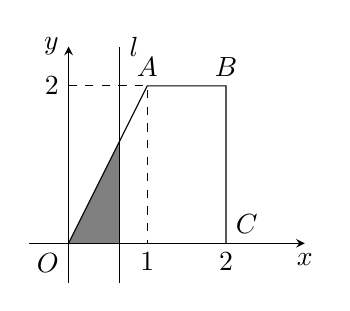
\begin{tikzpicture}[samples=200,>=stealth]
	\fill [gray] (0,0)--(0.65,0)--(0.65,1.3)--cycle;
	\draw [->] (-0.5,0)--(0,0) node [below left] {$O$} --(3,0) node [below] {$x$};
	\draw [->] (0,-0.5)--(0,2.5) node [left] {$y$};
	\draw (0,0)--(1,2) node [above] {$A$}--(2,2) node [above] {$B$}--(2,0) node [above right] {$C$};
	\draw (0.65,-0.5)--(0.65,2.5) node [right] {$l$};
	\draw [dashed] (0,2) node [left] {$2$} --(1,2)--(1,0) node [below] {$1$};
	\draw (2,0) node [below] {$2$};
	
	\end{tikzpicture}
\end{center}
则函数$S=f(t)$的图像大致为\blank{30}.
\fourch{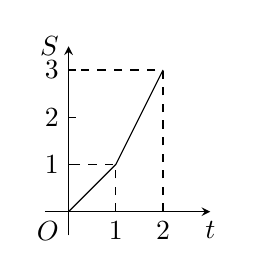
\begin{tikzpicture}[>=stealth]
	\draw [->] (-0.3,0)--(0,0) node [below left] {$O$} --(1.8,0) node [below] {$t$};
	\draw [->] (0,-0.3)--(0,2.1) node [left] {$S$};
	\draw (0.6,0) node [below] {$1$}--(0.6,0.1);
	\draw (1.2,0) node [below] {$2$}--(1.2,0.1);
	\draw (0,0.6) node [left] {$1$}--(0.1,0.6);
	\draw (0,1.2) node [left] {$2$}--(0.1,1.2);
	\draw (0,1.8) node [left] {$3$}--(0.1,1.8);
	\draw (0,0)--(0.6,0.6)--(1.2,1.8);
	\draw [dashed] (0.6,0)--(0.6,0.6)--(0,0.6);
	\draw [dashed] (1.2,0)--(1.2,1.8)--(0,1.8);
	\end{tikzpicture}}{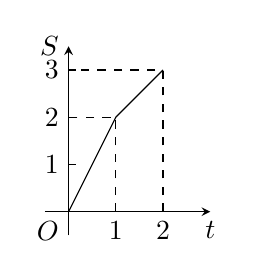
\begin{tikzpicture}[>=stealth]
	\draw [->] (-0.3,0)--(0,0) node [below left] {$O$} --(1.8,0) node [below] {$t$};
	\draw [->] (0,-0.3)--(0,2.1) node [left] {$S$};
	\draw (0.6,0) node [below] {$1$}--(0.6,0.1);
	\draw (1.2,0) node [below] {$2$}--(1.2,0.1);
	\draw (0,0.6) node [left] {$1$}--(0.1,0.6);
	\draw (0,1.2) node [left] {$2$}--(0.1,1.2);
	\draw (0,1.8) node [left] {$3$}--(0.1,1.8);
	\draw (0,0)--(0.6,1.2)--(1.2,1.8);
	\draw [dashed] (0.6,0)--(0.6,1.2)--(0,1.2);
	\draw [dashed] (1.2,0)--(1.2,1.8)--(0,1.8);
	\end{tikzpicture}}{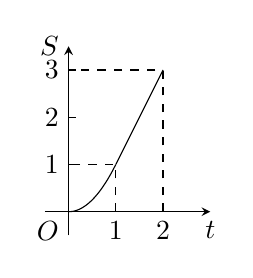
\begin{tikzpicture}[>=stealth,samples=200]
	\draw [->] (-0.3,0)--(0,0) node [below left] {$O$} --(1.8,0) node [below] {$t$};
	\draw [->] (0,-0.3)--(0,2.1) node [left] {$S$};
	\draw (0.6,0) node [below] {$1$}--(0.6,0.1);
	\draw (1.2,0) node [below] {$2$}--(1.2,0.1);
	\draw (0,0.6) node [left] {$1$}--(0.1,0.6);
	\draw (0,1.2) node [left] {$2$}--(0.1,1.2);
	\draw (0,1.8) node [left] {$3$}--(0.1,1.8);
	\draw [domain=0:1] plot ({\x*0.6},{\x*\x*0.6});
	\draw (0.6,0.6)--(1.2,1.8);
	\draw [dashed] (0.6,0)--(0.6,0.6)--(0,0.6);
	\draw [dashed] (1.2,0)--(1.2,1.8)--(0,1.8);
	\end{tikzpicture}}{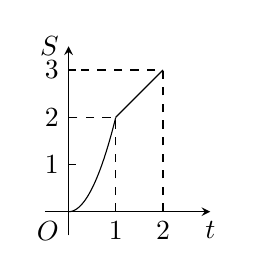
\begin{tikzpicture}[>=stealth,samples=200]
	\draw [->] (-0.3,0)--(0,0) node [below left] {$O$} --(1.8,0) node [below] {$t$};
	\draw [->] (0,-0.3)--(0,2.1) node [left] {$S$};
	\draw (0.6,0) node [below] {$1$}--(0.6,0.1);
	\draw (1.2,0) node [below] {$2$}--(1.2,0.1);
	\draw (0,0.6) node [left] {$1$}--(0.1,0.6);
	\draw (0,1.2) node [left] {$2$}--(0.1,1.2);
	\draw (0,1.8) node [left] {$3$}--(0.1,1.8);
	\draw [domain=0:1] plot ({\x*0.6},{2*\x*\x*0.6});
	\draw (0.6,1.2)--(1.2,1.8);
	\draw [dashed] (0.6,0)--(0.6,1.2)--(0,1.2);
	\draw [dashed] (1.2,0)--(1.2,1.8)--(0,1.8);
	\end{tikzpicture}}
\item {\tiny (003863)}求证: (1) 在所有周长相同的长方形中, 只有正方形的面积最大;\\
(2) 在所有面积相同的长方形中, 只有正方形的面积最小.
\item {\tiny (003864)}平面上定点$F$到定直线$l$的距离$|FM|=2$, $P$为该平面上的动点, 过$P$作直线$l$的垂线, 垂足为$Q$, 且$(\overrightarrow{PF}+\overrightarrow{PQ})\cdot (\overrightarrow{PF}-\overrightarrow{PQ})=0$.\\
(1) 试建立适当的平面直角坐标系, 求动点$P$的轨迹$C$的方程;\\
(2) 过点$F$的直线交轨迹$C$于$A,B$两点, 交直线$l$于点$N$, 已知$\overrightarrow{NA}=\lambda_1\overrightarrow{AF}$, $\overrightarrow{NB}=\lambda_2\overrightarrow{BF}$, 求证: $\lambda_1+\lambda_2$为定值.
\item {\tiny (003865)}集合$\{y|y=2^{-x}\}\cap\{y|y=\lg x, \ 0<x<100\}=$\blank{50}.
\item {\tiny (003866)}若$(1+\mathrm{i})z=a+\mathrm{i}$, $z$对应点在第二象限, 实数$a$的取值范围为\blank{50}.
\item {\tiny (003867)}如果$\left(\dfrac{1}{\sqrt{x}}-\dfrac{\sqrt{2}}{2}\right)^n$展开式第三项的二项式系数为$66$, 那么展开式第六项为\blank{50}.
\item {\tiny (003868)}已知$\sin x=\cos 2x, \ x\in\left(\dfrac{\pi}{2},\pi\right)$, 则$\tan x=$\blank{50}.
\item {\tiny (003869)}函数$f(x)=a^x+b \ (a>1, \ b<-1)$, 则$y=f^{-1}(x)$的图像一定不经过第\blank{50}象限.
\item {\tiny (003870)}函数$f(x)=3\sin (\omega x), \ omega>0$在区间$\left[-\dfrac{\pi}{3},\dfrac{\pi}{4}\right]$单调递增, 则$\omega$的取值范围为\blank{50}.
\item {\tiny (003871)}$\triangle OAB$中$OA=3$, $OB=4$, $C$是$AB$中点, 则$\overrightarrow OC\cdot \overrightarrow{AB}=$\blank{50}.
\item {\tiny (003872)}若$\{a,b\}\subseteq \{0,1,2,3,4,5,6\}$, 从复数$a+b\mathrm{i} \ (a\ne b)$中任取一个, 模小于等于$5$的概率为\blank{50}.
\item {\tiny (003873)}(理科)一个不透明的袋中装有白球、红球共$9$个($9$个球除颜色外其余完全相同), 经充分混合后, 从袋中随机摸出$2$球, 且摸出的$2$球中至少有一个是白球的概率为$\dfrac 56$, 现用$\xi$表示摸出的$2$个球中红球的个数, 则随机变量$\xi$的数学期望$E\xi=$\blank{50}.\\
(文科)一个不透明的袋中装有$5$个白球、$4$个红球($9$个球除颜色外其余完全相同), 经充分混合后, 从袋中随机摸出$3$球, 则摸出的$3$球中至少有一个是白球的概率为\blank{50}.
\item {\tiny (003874)}已知数列$\{a_n\}$的通项$a_n=\left(\dfrac 13\right)^n$, 数列$\{b_n\}$满足$b_1=-1$, $b_2=2$, $b_{n+2}=b_n, \ n\in \mathbf{N}^*$, 则$\displaystyle\lim_{n\to \infty}(a_1b_1+a_2b_2+\cdots+a_nb_n)=$\blank{50}.
\item {\tiny (003875)}在长方体$ABCD-A_1B_1C_1D_1$中, $B_1C$和$C_1D$与底面所成的角分别为$60^\circ$和$45^\circ$, 则异面直线$B_1C$和$C_1D$所成的角的余弦值为\blank{30}.
\fourch{$\dfrac{\sqrt{3}}6$}{$\dfrac{\sqrt{2}}{6}$}{$\dfrac{\sqrt{6}}{3}$}{$\dfrac{\sqrt{6}}{4}$}
\item {\tiny (003876)}(理科)甲、乙、丙、丁与小强一起比赛象棋, 每两人都要比赛一盘, 到现在为止, 甲已经赛了$4$盘, 乙赛了$3$盘, 丙赛了$2$盘, 丁赛了$1$盘, 则小强已经赛了\blank{30}.
\fourch{$4$盘}{$3$盘}{$2$盘}{$1$盘}\\
(文科)``$-2\le a\le 2$''是``实系数一元二次方程$x^2+ax+1=0$有虚根''的\blank{30}.
\fourch{充要条件}{必要不充分条件}{充分不必要条件}{既不充分也不必要条件}
\item {\tiny (003877)}已知点$P(x,y)$是直线$kx+y+4=0 \ (k>0)$上一动点, $PA,PB$是圆$C:x^2+y^2-2y=0$的两条切线, $A,B$是切点, 若四边形$PACB$($C$为圆心)面积的最小值为$2$, 则$k$的值为\blank{30}.
\fourch{$2$}{$\dfrac{\sqrt{21}}{2}$}{$2\sqrt{2}$}{$3$}
\item {\tiny (003878)}已知$\triangle ABC$的面积为$3$, 且满足$0\le \overrightarrow{AB}\cdot\overrightarrow{AC}\le 6$, 设$\overrightarrow{AB}$和$\overrightarrow{AC}$的夹角为$\theta$.\\
(1) 求$\theta$的取值范围;\\
(2) 求函数$f(\theta)=2\sin^2\left(\dfrac{\pi}{4}+\theta\right)-\sqrt{3}\cos 2\theta$的最大值与最小值.
\item {\tiny (003879)}(理科)在底面是直角梯形的四棱锥$S-ABCD$中, $\angle ABC=90^\circ$, $AD\parallel BC$, $SA\perp$平面$ABCD$, $SA=AB=BC=1$, $AD=\dfrac 12$, 求平面$SCD$与平面$SAB$所成的二面角的大小.\\
(文科)如图, 在体积为$\dfrac 13$的三棱锥$P-ABC$中, $PA\perp$平面$ABC$, $\angle ACB=90^\circ$, $PA=2AC=2BC$. 点$M,N$分别是$PB,PC$的中点.\\
(1) 求异面直线$AN$与$CM$所成的角的大小;\\
(2) 求$A$到平面$PBC$的距离.
\begin{center}
	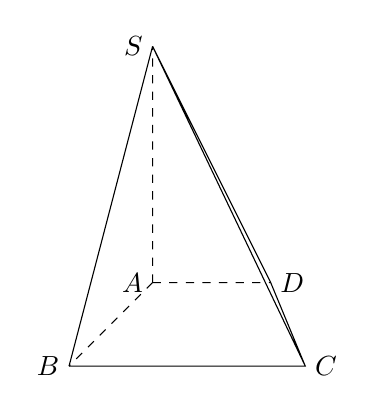
\begin{tikzpicture}
	\coordinate (A) at (0,0);
	\coordinate (D) at (1.5,0);
	\coordinate (B) at ({-sqrt(2)*3/4},{-sqrt(2)*3/4});
	\coordinate (C) at ({-sqrt(2)*3/4+3},{-sqrt(2)*3/4});
	\coordinate (S) at (0,3);
	\draw (B) --(C)--(S)--(D) node [right] {$D$} (S) node [left] {$S$}--(B) node [left] {$B$} (C) node [right] {$C$}--(D);
	\draw [dashed] (A) node [left] {$A$}--(B) (A)--(S) (A)--(D);
	\end{tikzpicture}
\end{center}
\begin{center}
	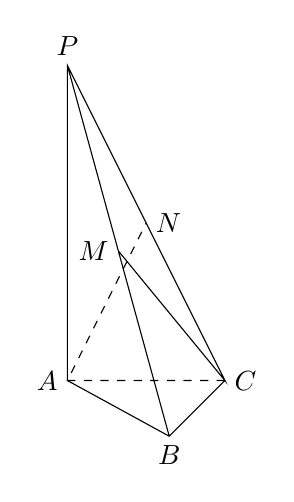
\begin{tikzpicture}
	\coordinate (A) at (0,0);
	\coordinate (C) at (2,0);
	\coordinate (P) at (0,4);
	\coordinate (B) at ({2-sqrt(2)/2},{-sqrt(2)/2});
	\coordinate (M) at ($(B)!0.5!(P)$);
	\coordinate (N) at ($(C)!0.5!(P)$);
	\draw (C) node [right] {$C$}--(B) node [below ] {$B$} --(A) node[left]{$A$}--(P) node [above]{$P$}--(C)--(M) node [left] {$M$} (P)--(B);
	\draw [dashed] (C)--(A)--(N) node [right] {$N$};
	
	\end{tikzpicture}
\end{center}
\item {\tiny (003880)}若$z=\sin\theta-\dfrac 35+\left(\cos\theta-\dfrac 45\right)\mathrm{i}$是纯虚数, 则$\tan\left(\theta-\dfrac{\pi}{4}\right)=$\blank{50}.
\item {\tiny (003881)}要使$y=x^2+4x \ (x\ge a)$有反函数, 则$a$的最小值为\blank{50}.
\item {\tiny (003882)}三个实数成等差数列, 首项是$9$. 若将第二项加$2$, 第三项加$20$可使得这三个数依次构成等比数列$\{a_n\}$, 则$a_3$的所有取值中的最小值是\blank{50}.
\item {\tiny (003883)}二项式$\left(x+\dfrac 1{2x}\right)^8$展开式中的二项式系数最大的项的系数为\blank{50}.
\item {\tiny (003884)}已知函数$y=f(x)$的定义域为$\{x|-3\le x\le 8, \ x\ne 5\}$, 值域为$\{y|-1\le y\le 2, \ y\ne 0\}$. 下列关于函数$y=f(x)$的说法: \textcircled{1} 当$x=-3$时, $y=-1$; \textcircled{2} 将$y=f(x)$的图像补上$(5,0)$, 得到的图像必定是一条连续的曲线; \textcircled{3} $y=f(x)$是$[-3,5)$上的单调函数; \textcircled{4} $y=f(x)$的图像与坐标轴只有一个交点. 其中正确的命题是\blank{50}.
\item {\tiny (003885)}点$P$是双曲线$\dfrac{x^2}{4}-y^2=1$的右支上一点, $M,N$分别是圆$(x+\sqrt{5})^2+y^2=1$和圆$(x-\sqrt{5})^2+y^2=1$上的点, 则$|PM|-|PN|$的最大值是\blank{50}.
\item {\tiny (003886)}设$\triangle ABC$的内角$A,B,C$所对的边分别为$a,b,c$, 若三边的长为连续的三个正整数, 且$A>B>C, \ A=2C$, 则$\sin A:\sin B:\sin C$为\blank{50}.
\item {\tiny (003887)}从集合$\{1,2,3,4,5,6,7,8,9\}$中任取两个不同的数, 则其中一个数恰是另一个数的$3$倍的概率为\blank{50}.
\item {\tiny (003888)}在$\triangle ABC$中, 边$AC=1$, $AB=2$, 角$A=\dfrac{2\pi}{3}$, 过$A$作$AP\perp BC$于$P$, 且$\overrightarrow{AP}=\lambda \overrightarrow{AB}+\mu \overrightarrow{A}$, 则$\lambda\mu=$\blank{50}.
\item {\tiny (003889)}已知函数$f(x)=\begin{cases}ax^2-2x-1, & x\ge 0,\\ x^2+bx+c, & x<0\end{cases}$是偶函数, 直线$y=t$与函数$y=f(x)$的图像自左向右依次交于四个不同点$A,B,C,D$. 若$AB=BC$, 则实数$t$的值为\blank{50}.
\item {\tiny (003890)}直线$\begin{vmatrix}
x & 0 & 1\\-1 & 2 & -1\\y & 1 & 1
\end{vmatrix}=0$的一个法向量是\blank{30}.
\fourch{$(2,3)$}{$(3,-2)$}{$(-2,3)$}{$(3,2)$}
\item {\tiny (003891)}已知平面$\alpha,\beta$和直线$m$, 给出条件: \textcircled{1} $m\parallel \alpha$; \textcircled{2} $m\perp \alpha$; \textcircled{3} $m\subseteq \alpha$; \textcircled{4} $\alpha\perp \beta$; \textcircled{5} $\alpha\parallel\beta$. 由给出的两个条件能推导出$m\parallel \beta$的是\blank{30}.
\fourch{\textcircled{1}\textcircled{4}}{\textcircled{1}\textcircled{5}}{\textcircled{2}\textcircled{4}}{\textcircled{3}\textcircled{5}}
\item {\tiny (003892)}已知函数$f(x)$是定义在$(-\infty,0)\cup (0,+\infty)$上的偶函数, 当$x>0$时, $f(x)=\begin{cases}
2^{|x-1|}-1, & 0<x\le 2,\\\dfrac 12f(x-2), & x>2,
\end{cases}$ 则函数$g(x)=4f(x)-1$的零点的个数为\blank{30}.
\fourch{$4$}{$6$}{$8$}{$10$}
\item {\tiny (003893)}已知圆方程为$x^2+y^2-2ax-4ay+4a^2+t=0 \ (a\ne 0)$.\\
(1) 若$t=\dfrac 12 a^2$, 确定无论$a$为何值均与圆相切的直线的方程;\\
(2) 若$t=a^2-4$, 确定无论$a$为何值被圆截得的弦长为$1$的直线的方程.
\item {\tiny (003894)}对于函数$f(x)=ax^2+(b+1)x+b-2 \ (a\ne 0)$, 若存在实数$x_0$, 使$f(x_0)=x_0$成立, 则称$x_0$为$f(x)$的不动点.\\
(1) 若对于任何实数$b$, 函数$f(x)$恒有两个相异的不动点, 求实数$a$的取值范围;\\
(2) 在(1)的条件下, 若函数$y=f(x)$的图像上$A,B$两点的横坐标是函数$f(x)$的不动点, 且直线$y=kx+\dfrac{1}{2a^2+1}$是线段$AB$的垂直平分线, 求实数$b$的取值范围.
\item {\tiny (003895)}已知椭圆$\dfrac{x^2}{t^2}+\dfrac{y^2}{5t}=1$的焦距为$2\sqrt{6}$, 则实数$t=$\blank{50}.
\item {\tiny (003896)}函数$y=x^2+4x \ (x<-3)$的反函数为\blank{50}.
\item {\tiny (003897)}已知$a$是实数, 若$A=\{x|ax^2+6x+9=0, \ x\in \mathbf{R}\}$中至多有一个元素, 则$a$的取值范围为\blank{50}.
\item {\tiny (003898)}已知球$O$的半径为$4$, $A,B$是球面上两点, $\angle AOB=45^\circ$, 则$A,B$两点的球面距离为\blank{50}.
\item {\tiny (003899)}设$A_n$为$(1+x)^{n+1}$的展开式中含$x^{n-1}$项的系数, $B_n$为$(1+x)^{n-1}$的展开式中二项式系数的和($n\in \mathbf{N}^*$), 则能使$A_n\ge B_n$成立的$n$的最大值是\blank{50}.
\item {\tiny (003900)}已知不等式$a\le \dfrac{x^2+2}{|x|}$对$x$取一切非零实数恒成立, 则$a$的取值范围是\blank{50}.
\item {\tiny (003901)}已知数列$\{a_n\}$是等差数列, 前$n$项和为$S_n$, 若$\overrightarrow{OP}=a_{1006}\overrightarrow{OA}+a_{1009}\overrightarrow{OB}$, 且$P,A,B$三点共线($O$不在该直线上), 则$S_{2014}=$\blank{50}.
\item {\tiny (003902)}已知函数$f(x)=\sin x+\tan \dfrac x2+x^3, \ x\in (-1,1)$, 则满足不等式$f(a-1)+f(2a-1)<0$的实数$a$的取值范围是\blank{50}.
\item {\tiny (003903)}有两个相同的直三棱柱, 高为$\dfrac 2a$, 底面三角形的三边长分别是$3a,4a,5a \ (a>0)$. 用它们拼成一个三棱柱或四棱柱, 在所有可能的情形中, 表面积最小的棱柱只有一种, 是一个三棱柱. 则实数$a$的取值范围是\blank{50}.
\item {\tiny (003904)}设$f(x)=a\sin 2x+b\cos 2x$, 其中$a,b\in \mathbf{R}$, $ab\ne 0$. 若$f(x)\le \left|f\left(\dfrac{\pi}{6}\right)\right|$对一切$x\in \mathbf{R}$恒成立, 则
\textcircled{1} $f\left(\dfrac{11\pi}{12}\right)=0$; \textcircled{2} $\left|f\left(\dfrac{7\pi}{12}\right)\right|<\left|f\left(\dfrac{\pi}{5}\right)\right|$; \textcircled{3} $f(x)$既不是奇函数也不是偶函数; \textcircled{4} $\left[k\pi+\dfrac{\pi}{6},k\pi+\dfrac{2\pi}{3}\right] \ (k\in \mathbf{Z})$是$f(x)$的单调区间; \textcircled{5} 存在经过点$(a,b)$的直线与函数$f(x)$的图像不相交. 
以上结论正确的是\blank{50}(写出所有正确结论的编号).
\item {\tiny (003905)}已知条件$p: |x+1|>2$, 条件$q: x>a$, 且$\bar{p}$是$\bar{q}$的充分不必要条件, 则$a$的取值范围可以是\blank{30}.
\fourch{$a\ge 1$}{$a\le 1$}{$a\ge -1$}{$a\le -3$}
\item {\tiny (003906)}已知$\{a_n\}$是以$a \ (a>0)$为首项以$q \ (-1<q<0)$为公比的等比数列, 设$A=\displaystyle\lim_{n\to \infty}(a_1+a_2+\cdots+a_n)$, $B=\displaystyle\lim_{n\to \infty}(a_1+a_2+a_3\cdots+a_{2n})$, $C=\displaystyle\lim_{n\to \infty}(a_1+a_3+a_5+\cdots+a_{2n-1})$, $D=\displaystyle\lim_{n\to \infty}(a_2+a_4+a_6+\cdots+a_{2n})$. 则$A,B,C,D$的大小关系是\blank{30}.
\fourch{$D<A<B<C$}{$D<A=B<C$}{$C<D<B<A$}{$A=B=C=D$}
\item {\tiny (003907)}设$f(x)$是定义在$\mathbf{R}$上的函数, 且对任意实数$x$, 恒有$f(x+2)=-3f(x)$. 当$x\in [0,2]$时, $f(x)=2x-x^2$, 则$f(0)+f(-1)+f(-2)+\cdots+f(-2014)=$\blank{30}.
\fourch{$-\dfrac 34(1-3^{1007})$}{$-\dfrac 34(1+3^{1007})$}{$-\dfrac 14\left(1-\dfrac{1}{3^{1007}}\right)$}{$-\dfrac 14\left(1+\dfrac{1}{3^{1007}}\right)$}
\item {\tiny (003908)}已知复数$z_1=\sqrt{3}+\mathrm{i}$, $|z_2|=2$, $z_1\cdot z_2^2$是虚部为正数的纯虚数.\\
(1) 求$z_1\cdot z_2^2$的模;\\
(2) 求复数$z_2$.
\item {\tiny (003909)}已知椭圆$C:\dfrac{x^2}{a^2}+\dfrac{y^2}{b^2}=1 \ (a>b>0)$的一个焦点坐标为$(1,0)$, 且长轴长是短轴长的$\sqrt{2}$倍.\\
(1) 求椭圆$C$的方程;\\
(2) 设$O$为坐标原点, 椭圆$C$与直线$y=kx+1$相交于两个不同的点$A,B$, 线段$AB$的中点为$P$, 若直线$OP$的斜率为$-1$, 求$\triangle AOB$的面积.
\item {\tiny (003910)}已知$\sin\alpha=\dfrac 5{13}$, $\alpha\in \left(\dfrac{\pi}{2},\dfrac{3\pi}{2}\right)$, 则$\tan\left(\dfrac{\pi}{4}+\alpha\right)$的值是\blank{50}.
\item {\tiny (003911)}已知函数$f(x)=\begin{cases}
2^x-1, & x\ge 0,\\ -x^2-2x, & x<0,
\end{cases}$ 若$f(a)=1$, 则实数$a$的值是\blank{50}.
\item {\tiny (003912)}已知$x,y\in \mathbf{R}$, 且$x+2y=1$, 则$2^x+4^y$的最小值是\blank{50}.
\item {\tiny (003913)}设点$P(x_0,y_0)$是函数$y=\tan x$与$y=-x \ (x>0)$的图像的一个交点, 则$(x_0^2+1)(\cos 2x_0+1)=$\blank{50}.
\item {\tiny (003914)}投掷一枚质地均匀的骰子两次, 若第一次面向上的点数小于第二次面向上的点数, 我们称其为正实验; 若第二次面上上的点数小于第一次面向上的点数, 我们称其为负实验; 若两次面向上的点数相等, 我们称其为无效实验. 那么一个人投掷该骰子两次后出现无效实验的概率是\blank{50}.
\item {\tiny (003915)}向量$\overrightarrow{a}=(3,-4)$, 向量$\left|\overrightarrow b\right|=2$, 若$\overrightarrow a\cdot \overrightarrow b=-5$, 那么向量$\overrightarrow a$, $\overrightarrow b$的夹角是\blank{50}.
\item {\tiny (003916)}下图所示为一个判断直线$Ax+By+C=0$与圆$(x-a)^2+(y-b)^2=r^2$的位置关系的程序框图的一部分, 在``$?$''处应填上\blank{50}.
\begin{center}
	\begin{tikzpicture}[>=stealth]
	\draw [->] (-0.4,0)--(0,0);
	\draw (-0.3,-0.3)--(0.3,0.3)--(2.7,0.3)--(2.1,-0.3)--cycle;
	\draw (1.2,0) node {输入$A,B,C$};
	\draw [->] (2.4,0)--(2.8,0);
	\draw (2.5,-0.3)--(3.1,0.3)--(5.5,0.3)--(4.9,-0.3)--cycle;
	\draw (4,0) node {输入$a,b,r$};
	\draw [->] (5.2,0)--(5.6,0);
	\draw (5.6,-0.6) rectangle (8.6,0.6);
	\draw (7.1,0) node {$d=\dfrac{|\phantom{11}?\phantom{11}|}{\sqrt{A^2+B^2}}$};
	\draw [->] (8.6,0)--(9,0);
	\draw (9,0)--(10,0.5)--(11,0)--(10,-0.5)--cycle;
	\draw (10,0) node {$d=r$};
	\draw [->] (11,0)--(11.4,0);
	\draw (11.2,0) node [above] {是};
	\draw [->] (10,-0.5)node [below right] {否}--(10,-0.9); 
	\draw (11.1,-0.3)--(11.7,0.3)--(15.1,0.3)--(14.5,-0.3)--cycle;
	\draw (13.2,0) node {输出直线与圆相切};
	\draw[->] (14.8,0)--(15.2,0);
	\end{tikzpicture}
\end{center}
\item {\tiny (003917)}已知曲线$C_1,C_2$的极坐标方程分别为$\rho=4\cos\theta \ \left(\rho\ge 0, \ 0\le \theta<\dfrac{\pi}{2}\right)$, $\rho\cos\theta=3$, 则曲线$C_1$与$C_2$交点的极坐标为\blank{50}.
\item {\tiny (003918)}椭圆两焦点为$F_1(-4,0)$, $F_2(4,0)$, $P$在椭圆上, 若$\triangle PF_1F_2$的面积的最大值为$12$, 则该椭圆的标准方程为\blank{50}.
\item {\tiny (003919)}将正整数按下表的规律排列, 把行与列交叉处的一个数称为某行某列的数, 记作$a_{i,j} \ (i,j\in \mathbf{N}^*)$, 如第$2$行第$4$列的数是$15$, 记作$a_{2,4}=15$, 则$a_{12,14}=$\blank{50}.
\begin{center}
\begin{tabular}{cccccccc}
$1$ & $4$ & $5$ & $16$ & $17$ & $36$ & $\cdots$\\
$2$ & $3$ & $6$ & $15$ & $18$ & $35$ & $\cdots$\\
$9$ & $8$ & $7$ & $14$ & $19$ & $34$ & $\cdots$\\
$10$ & $11$ & $12$ & $13$ & $20$ & $33$ & $\cdots$\\
$25$ & $24$ & $23$ & $22$ & $21$ & $32$ & $\cdots$\\
$26$ & $27$ & $28$ & $29$ & $30$ & $31$ & $\cdots$\\
$\cdots$ & $\cdots$ & $\cdots$ & $\cdots$ & $\cdots$ & $\cdots$ & $\cdots$
\end{tabular}
\end{center}
\item {\tiny (003920)}设矩形的长为$a$, 宽为$b$, 其比满足$b:a=\dfrac{\sqrt{5}-1}{2}\approx 0.618$, 这种矩形给人以美感, 称为黄金矩形. 黄金矩形常应用于工艺品设计中. 下面是某工艺品厂随机抽取两个批次的初加工矩形宽度与长度的比值样本:
\begin{center}
\begin{tabular}{cccccc}
甲批次: & $0.598$ & $0.625$ & $0.628$ & $0.595$ & $0.639$\\
乙批次: & $0.618$ & $0.613$ & $0.592$ & $0.622$ & $0.620$
\end{tabular}
\end{center}
跟据上述两个样本来估计两个批次的总体平均数, 与标准值$0.618$作比较, 正确结论是\blank{30}
\twoch{甲批次的总体平均数与标准值更接近}{甲批次的总体平均数与标准值更接近}{两个批次总体平均数与标准值接近程度相同}{两个批次总体平均数与标准值接近程度不能确定}
\item {\tiny (003921)}已知函数$f(x)=\dfrac{x}{1+|x|} \ (x\in \mathbf{R})$时, 则下列结论{\bf 不正确}的是\blank{30}.
\onech{任意$x\in \mathbf{R}$, 等式$f(-x)+f(x)=0$恒成立}{存在$m\in (0,1)$, 使得方程$|f(x)|=m$有两个不等实数根}{对任意$x_1,x_2\in \mathbf{R}$, 若$x_1\ne x_2$, 则一定有$f(x_1)\ne f(x_2)$}{存在$k\in (1,+\infty)$, 使得函数$g(x)=f(x)-kx$在$\mathbf{R}$上三个零点}
\item {\tiny (003922)}给出下列类比推理命题($\mathbf{R}$为实数集, $\mathbf{C}$为复数集, $M$为平面向量集), 其中类比结论正确的是\blank{30}.
\onech{由``若$a\in \mathbf{R}$, 则$a^2=|a|^2$''类比推出``若$a\in \mathbf{C}$, 则$a^2=|a|^2$''}{由``若$a,b\in \mathbf{R}$, 且$a-b=0$, 则$a=b$''类比推出``若$\overrightarrow{a},\overrightarrow{b}\in \mathbf{M}$, 且$\overrightarrow a-\overrightarrow b=\overrightarrow 0$, 则$\overrightarrow a=\overrightarrow b$''}{由``若$a,b\in \mathbf{R}$, 且$a^2+b^2=0$, 则$a=0$或$b=0$''类比推出``若$a,b\in \mathbf{C}$, 且$a^2+b^2=0$, 则$a=0$或$b=0$''}{由``若$a,b\in \mathbf{R}$, 且$a\cdot b=0$, 则$a=0$或$b=0$''类比推出``若$\overrightarrow a, \overrightarrow b\in \mathbf{M}$, 且$\overrightarrow a\cdot \overrightarrow b=0$, 则$\overrightarrow a=\overrightarrow 0$或$\overrightarrow b=\overrightarrow 0$''}
\item {\tiny (003923)}(1) 设$x,y$是不全为零的实数, 试比较$2x^2+y^2$与$x^2+xy$的大小;\\
(2) 设$a,b,c$为正数, 且$a^2+b^2+c^2=1$, 求证: $\dfrac 1{a^2}+\dfrac 1{b^2}+\dfrac 1{c^2}-\dfrac{2(a^3+b^3+c^3)}{abc}\ge 3$.
\item {\tiny (003924)}数列$\{a_n\}$的首项为$1$, 前$n$项和是$S_n$, 存在常数$A,B$使$a_n+S_n=An+B$对任意正整数$n$都成立.\\
(1) 设$A=0$, 求证: 数列$\{a_n\}$是等比数列;\\
(2) 设数列$\{a_n\}$是等差数列, 若$p<q$, 且$\dfrac{1}{S_p}+\dfrac{1}{S_q}=\dfrac{1}{S_{11}}$, 求$p,q$的值;\\
(3) 设$A>0$, $A\ne 1$, 且$\dfrac{a_n}{a_{n+1}}\le M$对任意正整数$n$都成立, 求$M$的取值范围.
\item {\tiny (003925)}已知集合$A=\{x|x^2-2x\le 0 \}$, $B=\{x|-1<x<1\}$, 则$A\cap B=$\blank{50}.
\item {\tiny (003926)}若复数$(1+\mathrm{i})(a+\mathrm{i})$是实数($\mathrm{i}$是虚数单位), 则实数$a$的值\blank{50}.
\item {\tiny (003927)}已知数列$\{a_n\}$是等差数列, 若$a_4+2a_6+a_8=12$, 则该数列前$11$项的和为\blank{50}.
\item {\tiny (003928)}阅读下图的程序框图, 若输入$n=5$, 则输出$k$的值为\blank{50}.
\begin{center}
	\begin{tikzpicture}[>=stealth]
	\draw (0,-0.3)--(1,-0.3) arc (-90:90:0.3)--(0,0.3) arc (90:270:0.3);
	\draw (0.5,0) node {开始};
	\draw [->] (1.3,0)--(1.7,0);
	\draw (1.4,-0.3)--(2,0.3)--(3.6,0.3)--(3,-0.3)--cycle;
	\draw (2.5,0) node {输入$n$};
	\draw [->](3.3,0)--(3.7,0);
	\draw (3.7,0.3) rectangle (4.9,-0.3);
	\draw (4.3,0) node {$k=0$};
	\draw [->] (4.9,0)--(5.3,0);
	\draw (5.3,0.3) rectangle (7.1,-0.3);
	\draw (6.2,0) node {$n=3n+1$};
	\draw [->] (7.1,0)--(7.5,0);
	\draw (7.5,0)--(8.4,0.5)--(9.3,0)--(8.4,-0.5)--cycle;
	\draw (8.4,0) node {$n>150$};
	\draw [->] (9.3,0) --(9.7,0); 
	\draw (9.5,0) node [above]{是};
	\draw [->] (8.4,-0.5) node [below right] {否}--(8.4,-0.9)--(7.1,-0.9);
	\draw (7.1,-1.2) rectangle (5.3,-0.6);
	\draw (6.2,-0.9) node {$k=k+1$};
	\draw [->] (5.3,-0.9)--(3.5,-0.9)--(3.5,0);
	\draw (9.4,-0.3)--(10,0.3)--(11.8,0.3)--(11.2,-0.3)--cycle;
	\draw (10.6,0) node {输出$k,n$};
	\draw [->] (11.5,0)--(11.9,0);
	\draw (12.2,0.3) arc (90:270:0.3)--(13.2,-0.3) arc (-90:90:0.3)--cycle;
	\draw (12.7,0) node {结束};
	\end{tikzpicture}
\end{center}
\item {\tiny (003929)}如图所示, 已知正方体$ABCD-A_1B_1C_1D_1$的棱长为$2$, 长为$2$的线段$MN$的一个端点$M$在棱$DD_1$上运动, 另一端点$N$在正方形$ABCD$内运动, 则$MN$的中点的轨迹的面积为\blank{50}.
\begin{center}
	\begin{tikzpicture}
	\draw (0,0) node [below left] {$A$}--(1.5,0) node [below right] {$B$}--({1.5+0.375*sqrt(2)},{0.375*sqrt(2)}) node [right] {$C$}--({1.5+0.375*sqrt(2)},{1.5+0.375*sqrt(2)}) node [above right] {$C_1$}--({0.375*sqrt(2)},{1.5+0.375*sqrt(2)}) node [above left] {$D_1$} --(0,1.5) node [left] {$A_1$}--(1.5,1.5) node [right] {$B_1$}--(1.5,0) (1.5,1.5)--({1.5+0.375*sqrt(2)},{1.5+0.375*sqrt(2)}) (0,0)--(0,1.5);
	\draw [dashed] (0,0)--({0.375*sqrt(2)},{0.375*sqrt(2)}) node [left] {$D$}--({1.5+0.375*sqrt(2)},{0.375*sqrt(2)}) ({0.375*sqrt(2)},{0.375*sqrt(2)})--({0.375*sqrt(2)},{1.5+0.375*sqrt(2)});
	\draw [dashed] ({0.375*sqrt(2)},{0.375*sqrt(2)+0.9}) coordinate (M) node [below left] {$M$}--({0.375*sqrt(2)+0.6*sqrt(2)-0.3},{0.375*sqrt(2)-0.3}) coordinate (N) node [right] {$N$};
	\coordinate (P) at ($(M)!0.5!(N)$);
	\filldraw (P) circle (0.02) node [right] {$P$};
	\end{tikzpicture}
\end{center}
\item {\tiny (003930)}以抛物线$C:y^2=8x$上的一点$A$为圆心作圆, 若该圆经过抛物线$C$的顶点和焦点, 那么该圆的方程为\blank{50}.
\item {\tiny (003931)}$\triangle ABC$的三个内角$A,B,C$所对边的长分别为$a,b,c$, 已知$c=3$, $C=\dfrac{\pi}{3}$, $a=2b$, 则$b$的值为\blank{50}.
\item {\tiny (003932)}若函数$y=\cos(\omega x+\varphi) \ (\omega>0, \ 0<\varphi<\pi)$为奇函数, $A,B$分别为相邻的两个最高点, 并且两点间的距离为$4$, 则该函数的图像的对称轴为\blank{50}.
\item {\tiny (003933)}若称横坐标、纵坐标都为整数的点为``整点'', 过曲线$y=\sqrt{100-x^2}$上任意两个整点作直线, 则倾斜角不小于$30^\circ$的直线条数为\blank{50}.
\item {\tiny (003934)}数列$\{a_n\}$满足$a_1=1$, $\sqrt{\dfrac{1}{a_n^2}+4}=\dfrac{1}{a_{n+1}}$, 记数列$\{a_n^2\}$前$n$项的和为$S_n$, 若$S_{2n+1}-S_n\le \dfrac t{30}$对任意的$n\in \mathbf{N}^*$恒成立, 则正整数$t$的最小值为\blank{50}.
\item {\tiny (003935)}设函数$f(x)=\cos^2\left(x+\dfrac{\pi}{4}\right)-\sin^2\left(x+\dfrac{\pi}{4}\right)$, $x\in \mathbf{R}$, 则函数$f(x)$是\blank{30}.
\twoch{最小正周期为$\pi$的奇函数}{最小正周期为$\pi$的偶函数}{最小正周期为$\dfrac{\pi}{2}$的奇函数}{最小正周期为$\dfrac{\pi}{2}$的偶函数}
\item {\tiny (003936)}函数$y=\ln(\cos x) \ \left(-\dfrac{\pi}{2}<x<\dfrac{\pi}{2}\right)$的大致图像是\blank{30}.
\fourch{\begin{tikzpicture}[samples=200,>=stealth]
	\draw [->](-1.5,0)--(0,0) node [above left] {$O$}--(1.5,0) node [below] {$x$};
	\draw [->](0,-1.5)--(0,1.5) node [left] {$y$};
	\draw [dashed] (-1,-1.5)--(-1,1.5) (1,-1.5)--(1,1.5);
	\draw (-1,0) node [below left] {$-\dfrac{\pi}{2}$};
	\draw (1,0) node  [below right] {$\dfrac{\pi}{2}$};
	\draw [domain=-75:75] plot ({\x/90},{ln(cos(\x))});
	\end{tikzpicture}}{\begin{tikzpicture}[samples=200,>=stealth]
	\draw [->](-1.5,0)--(0,0) node [above left] {$O$}--(1.5,0) node [below] {$x$};
	\draw [->](0,-1.5)--(0,1.5) node [left] {$y$};
	\draw [dashed] (-1,-1.5)--(-1,1.5) (1,-1.5)--(1,1.5);
	\draw (-1,0) node [below left] {$-\dfrac{\pi}{2}$};
	\draw (1,0) node  [below right] {$\dfrac{\pi}{2}$};
	\draw [domain=-75:0] plot ({\x/90},{ln(cos(\x))});
	\draw [domain=0:75] plot ({\x/90},{-ln(cos(\x))});
	\end{tikzpicture}}{\begin{tikzpicture}[samples=200,>=stealth]
	\draw [->](-1.5,0)--(0,0) node [below left] {$O$}--(1.5,0) node [below] {$x$};
	\draw [->](0,-1.5)--(0,1.5) node [left] {$y$};
	\draw [dashed] (-1,-1.5)--(-1,1.5) (1,-1.5)--(1,1.5);
	\draw (-1,0) node [below left] {$-\dfrac{\pi}{2}$};
	\draw (1,0) node  [below right] {$\dfrac{\pi}{2}$};
	\draw [domain=-75:0] plot ({\x/90},{-ln(cos(\x))});
	\draw [domain=0:75] plot ({\x/90},{ln(cos(\x))});
	\end{tikzpicture}}{\begin{tikzpicture}[samples=200,>=stealth]
	\draw [->](-1.5,0)--(0,0) node [below left] {$O$}--(1.5,0) node [below] {$x$};
	\draw [->](0,-1.5)--(0,1.5) node [left] {$y$};
	\draw [dashed] (-1,-1.5)--(-1,1.5) (1,-1.5)--(1,1.5);
	\draw (-1,0) node [below left] {$-\dfrac{\pi}{2}$};
	\draw (1,0) node  [below right] {$\dfrac{\pi}{2}$};
	\draw [domain=-75:75] plot ({\x/90},{-ln(cos(\x))});
	\end{tikzpicture}}
\item {\tiny (003937)}在实数集$\mathbf{R}$上定义运算$\otimes: x\otimes y=2x^2+y^2+1-y$, 则满足$x\otimes y=y\otimes x$的实数对$(x,y)$在平面直角坐标系中对应点的轨迹为\blank{30}.
\fourch{双曲线}{一条直线}{两条直线}{以上都不对}
\item {\tiny (003938)}如图, 该几何体由半圆柱体与直三棱柱构成, 半圆柱体底面直径$BC=4$, $AB=AC$, $\angle BAC=90^\circ$, $D$为半圆弧$B_1C_1$的中点, 若异面直线$BD$和$AB_1$所成的角的大小为$\arccos\dfrac 23$, 求:\\
(1) 该几何体的体积;\\
(2) 直线$AC$与平面$ACC_1A_1$所成的角的大小.
\begin{center}
	\begin{tikzpicture}
	\draw (-2,-2) node [left]{$B$} --(-2,2) node [left] {$B_1$} --(2,2) node [right]{$C_1$}--(2,-2) node [right] {$C$};
	\draw [dashed] (-2,-2)--(2,-2);
	\draw (2,2) arc (0:180:2 and 1);
	\draw [dashed] (2,-2) arc (0:180: 2 and 1);
	\path (2,2) arc (0:120:2 and 1) coordinate (D);
	\coordinate (A) at ($(0,0)!-1!(D)$);
	\coordinate (A1) at ($(0,2)!-1!(D)$);
	\draw [dashed] (D) node [above left] {$D$}--(A) node [below right]{$A$} (-2,-2)--(D);
	\draw (-2,-2)--(A)--(2,-2) (A)--(A1) node [right] {$A_1$} (-2,2)--(A1)--(2,2) (A)--(-2,2);
	\end{tikzpicture}
\end{center}
\item {\tiny (003939)}设数列$\{a_n\}$的前$n$项和为$S_n$, 对任意的正整数$n$, 都有$a_n=5S_n+1$成立, 记$b_n=\dfrac{4+a_n}{1-a_n} \ (n\in\mathbf{N}^*)$.\\
(1) 求数列$\{b_n\}$的通项公式;\\
(2) 记$c_n=b_{2n}-b_{2n-1} \ (n\in \mathbf{N}^*)$, 设数列$\{c_n\}$的前$n$项和为$T_n$, 求证: 对任意正整数$n$都有$T_n<\dfrac 32$.
\item {\tiny (003940)}已知集合$A=\{x|x=a+(a^2-1)\mathrm{i}\}$($a\in \mathbf{R}$, $\mathrm{i}$是虚数单位), 若$A\subseteq \mathbf{R}$, 则$a=$\blank{50}.
\item {\tiny (003941)}在正方体$ABCD-A_1B_1C_1D_1$中, $M$和$N$分别为$A_1B_1$和$BB_1$的中点, 那么直线$AM$与$CN$所成角的余弦值是\blank{50}.
\item {\tiny (003942)}计算$1-3\mathrm{C}_{10}^1+9\mathrm{C}_{10}^2-27\mathrm{C}_{10}^3+\cdots-3^9\mathrm{C}_{10}^9+3^{10}=$\blank{50}.
\item {\tiny (003943)}在$\triangle ABC$中, 角$A,B,C$所对的边分别为$a,b,c$. 若$a=\sqrt{2}$, $b=2$, $\sin B+\cos B=\sqrt{2}$, 则角$A$的大小为\blank{50}.
\item {\tiny (003944)}(理科)已知两曲线参数方程分别为$\begin{cases}x=\sqrt{5}\cos\theta,\\y=\sin\theta,\end{cases} (0\le \theta<\pi)$和$\begin{cases}
x=\dfrac 54 t^2, \\ y=t, \end{cases}
(t\in \mathbf{R})$, 它们的焦点坐标为\blank{50}.
\item {\tiny (003945)}从抛物线$y^2=4x$上一点$P$引抛物线的垂线, 垂足为$M$, 且$|PM|=5$, 设抛物线的焦点为$F$, 则$\triangle MPF$的面积为\blank{50}.
\item {\tiny (003946)}在$\triangle ABC$中, 点$O$是$BC$的中点, 过点$O$的直线分别交直线$AB,AC$于不同的两点$M,N$, 若$\overrightarrow{AB}=m\overrightarrow{AM}, \overrightarrow{AC}=n\overrightarrow{AN}$, $m>0$, $n>0$, 则$\dfrac 1m+\dfrac 4n$的最小值为\blank{50}.
\item {\tiny (003947)}已知$3$名志愿者在$10$月$1$日至$10$月$5$日期间参加$2013$年国庆节志愿者活动工作.\\
(文科)若每名志愿者在$5$天中任选一天参加社区服务工作, 且各志愿者的选择互不影响, 则$3$名志愿者恰好连续$3$天参加社区服务工作的概率为\blank{50}.\\
(理科)若每名志愿者在这$5$天中任选两天参加社区服务工作, 且各志愿者的选择互不影响, 以$\xi$表示这$3$名志愿者在$10$月$1$日参加志愿者服务工作的人数, 则随机变量$\xi$的数学期望为\blank{50}.
\item {\tiny (003948)}已知对于任意非零实数$m$, 不等式$|5m-3|+|3-4m|\ge |m|\left(x-\dfrac 2x\right)$恒成立, 则实数$x$的取值范围是\blank{50}.
\item {\tiny (003949)}已知圆的半径为$1$, $PA,PB$为该圆的两条切线, $A,B$为切点, 那么$\overrightarrow{PA}\cdot\overrightarrow{PB}$的最小值为\blank{50}.
\item {\tiny (003950)}若$m,n$为两条不同的直线, $\alpha,\beta$为两个不同的平面, 则以下命题正确的是\blank{30}.
\twoch{若$m\parallel \alpha$, $n\parallel\alpha$, 则$m\parallel n$}{若$m\parallel \beta$, $\alpha\parallel\beta$, 则$m\parallel\alpha$}{若$m\parallel n$, $m\perp \alpha$, 则$n\perp \alpha$}{若$\alpha\cap\beta=m$, $m\perp n$, 则$n\perp\alpha$}
\item {\tiny (003951)}双曲线$\dfrac{x^2}{a^2}-\dfrac{y^2}{b^2}=1$的左焦点为$F_1$, 顶点为$A_1,A_2$, $P$是该双曲线右支上任意一点, 则分别以线段$PF_1,A_1A_2$为直径的两圆一定\blank{30}.
\fourch{相交}{内切}{外切}{相离}
\item {\tiny (003952)}方程$x^2+\sqrt{2}x-1=0$的解可视为函数$y=x+\sqrt{2}$的图像与函数$y=\dfrac 1x$的图像交点的横坐标, 若$x^4+ax-4=0$的各个实根$x_1,x_2,\cdots,x_k \ (k\le 4)$所对应的点$\left(x_i,\dfrac{4}{x_i}\right) \ (i=1,2,\cdots,k)$均在直线$y=x$的同侧, 则实数$a$的取值范围是\blank{30}.
\fourch{$(-\infty,-6)$}{$(6,+\infty)$}{$[-6,6]$}{$(-\infty,-6)\cup (6,+\infty)$}
\item {\tiny (003953)}已知集合$M$是满足下列性质的函数$f(x)$的全体, 存在非零常数$T$, 对任意$x\in \mathbf{R}$, 有$f(x+T)=Tf(x)$成立.\\
(1) 函数$f(x)=x$是否属于集合$M$? 说明理由;\\
(2) 设$f(x)\in M$, 且$T=2$, 已知当$1<x<2$时, $f(x)=x+\ln x$, 求当$-3<x<-2$时, $f(x)$的解析式.
\item {\tiny (003954)}在数列$\{a_n\}$中, 对于任意$n\in \mathbf{N}^*$, 等式$a_1+2a_2+2^2a_3+\dots+2^{n-1}a_n=(n\cdot 2^n-2^n+1)b$成立, 其中常数$b\ne 0$.\\
(1) 求$a_1,a_2$的值;\\
(2) 求证: 数列$\{2^{a_n}\}$为等比数列;\\
(3) 关于$n$的不等式$\dfrac{1}{a_2}+\dfrac{1}{a_4}+\dfrac{1}{a_8}+\cdots+\dfrac{1}{a_{2^n}}>\dfrac{c}{a_1} \ (c\in \mathbf{R})$的解集为$\{n|n\ge 3, \ n\in \mathbf{N}^*\}$, 求$b$和$c$应满足的条件.
\item {\tiny (003955)}复数$\dfrac{(1+\mathrm{i})^2}{1-\sqrt{3}\mathrm{i}}$的模是\blank{50}.
\item {\tiny (003956)}若$\begin{vmatrix}a_1 & b_1 & c_1\\1 & 2 & 3\\4 & 5 & 6\end{vmatrix}=a_1A_1+b_1B_1+c_1C_1$, 则$B_1$化简后的最后结果等于\blank{50}.
\item {\tiny (003957)}已知集合$P=\{a,-1\}$, $Q=\{x|x^2-1<0, \ x\in \mathbf{Z}\}$, 如果$P\cap Q\ne\varnothing$, 则实数$a=$\blank{50}.
\item {\tiny (003958)}若圆锥的侧面展开图是弧长为$2\pi$cm, 半径为$\sqrt{2}$cm的扇形, 则该圆锥的体积为\blank{50}cm$^3$.
\item {\tiny (003959)}已知角$\alpha$的终边上一点的坐标为$\left(\sin\dfrac{2\pi}{3},\cos\dfrac{2\pi}{3}\right)$, 则角$\alpha$的最小正值为\blank{50}.
\item {\tiny (003960)}(理科)已知随机变量$\xi$的分布列如下表, 则随机变量$10\xi+1$的均值是\blank{50}.
\begin{center}
\begin{tabular}{|c|c|c|c|c|c|}
\hline
$x$ & $1$ & $2$ & $3$ & $4$ & $5$\\ \hline
$P(\xi=x)$ & $0.1$ & $a$ & $0.4$ & $0.1$ & $0.2$\\ \hline
\end{tabular}
\end{center}
\item {\tiny (003961)}若函数$f(x)=2\cos\left(\dfrac{\pi}{3}x-\dfrac{\pi}{6}\right) \ (-1<x<5)$的图像与$x$轴交于点$A$, 过点$A$的直线$l$与函数的图像交于另外两点$B,C$. $O$是坐标原点, 则$(\overrightarrow{OB}+\overrightarrow{OC})\cdot\overrightarrow{OA}=$\blank{50}.
\item {\tiny (003962)}设$(1+x)+(1+x)^2+\cdots+(1+x)^n=a_0+a_1x+a_2x^2+\cdots+a_nx^n, \ n\in \mathbf{N}^*$, 若$a_1+a_2+\cdots+a_{n-1}=61-n$, 则$n=$\blank{50}.
\item {\tiny (003963)}若存在$x\in [0,1]$, 使不等式$x^2+x\ge a^2+a$成立, 则实数$a$的取值范围是\blank{50}.
\item {\tiny (003964)}$F$为双曲线$C: \dfrac{x^2}{64}-\dfrac{y^2}{16}=1$的左焦点, 双曲线$C$上的点$P_i$与$P_{7-i} \ (i=1,2,3)$关于$y$轴对称, 且$P_1,P_2,P_3$在双曲线的右支上, 则$|P_1F|+|P_2F|+|P_3F|-|P_4F|-|P_5F|-|P_6F|$的值是\blank{50}.
\item {\tiny (003965)}(文科)已知非零实数$a,b$满足$a>b$. 则下列不等式中成立的是\blank{30}.
\fourch{$a^2>b^2$}{$\dfrac 1a<\dfrac 1b$}{$a^2b>ab^2$}{$\dfrac{a}{b^2}>\dfrac{b}{a^2}$}\\
(理科)对任意的实数$\alpha,\beta$, 下列等式恒成立的是\blank{30}.
\twoch{$2\sin\alpha\cdot\cos\beta=\sin(\alpha+\beta)+\sin(\alpha-\beta)$}{$2\cos\alpha\cdot\sin\beta=\sin(\alpha+\beta)+\cos(\alpha-\beta)$}{$\cos\alpha+\cos\beta=2\sin\dfrac{\alpha+\beta}{2}\cdot\sin\dfrac{\alpha-\beta}{2}$}{$\cos\alpha-\cos\beta=2\cos\dfrac{\alpha+\beta}{2}\cdot\cos\dfrac{\alpha-\beta}{2}$}
\item {\tiny (003966)}(理科)已知函数$f(x)$是定义在$\mathbf{R}$上的单调递减函数且为奇函数, 数列$\{a_n\}$是等差数列, $a_{1007}>0$, 则$f(a_1)+f(a_2)+f(a_3)+\cdots+f(a_{2012})+f(a_{2013})$的值\blank{30}.
\fourch{恒为正数}{恒为负数}{恒为$0$}{可正可负}
\item {\tiny (003967)}已知$A,B$为平面内两定点, 过该平面内动点$M$作直线$AB$的垂线, 垂足为$N$. 若$\overrightarrow{MN}^2=\lambda \overrightarrow{AN}\cdot\overrightarrow{NB}$, 其中$\lambda$为常数, 则动点$M$的轨迹不可能是\blank{50}.
\fourch{圆}{椭圆}{抛物线}{双曲线}
\item {\tiny (003968)}(文科)如图, 在正三棱柱$ABC-A_1B_1C_1$中, $AA_1=6$, 异面直线$BC_1$与$AA_1$所成角的大小为$\dfrac{\pi}{6}$, 求该三棱柱的体积和表面积.\\
(理科)在等腰直角三角形$ABC$中, $\angle A=90^\circ$, $BC=6$, $D,E$分别是$AC,AB$上的点, $CD=BE=\sqrt{2}$, $O$为$BC$的中点. 将$\angle ADE$沿$DE$折起, 得到如图所示的四棱锥$A'-BCDE$, 其中$A'O=\sqrt{3}$.\\
(1) 证明: $A'O\perp$平面$BCDE$;\\
(2) 求二面角$A'-CD-B$的平面角的余弦值.
\begin{center}
	\begin{tikzpicture}
	\draw [dashed](0,0) node [left] {$A$}--({2*sqrt(3)},0) node [right] {$C$};
	\path (1,-1) coordinate (B);
	\path (1,3) coordinate (B1);
	\draw (0,0)--(B)--({2*sqrt(3)},0);
	\draw (B) node [below] {$B$}--(B1) node [below right] {$B_1$};
	\draw (0,0)--(0,4) node [left] {$A_1$}--(B1)--({2*sqrt(3)},4) node [right] {$C_1$}--(0,4) ({2*sqrt(3)},0)--({2*sqrt(3)},4)--(B);
	\end{tikzpicture}
	
	\begin{tikzpicture}
	\draw (-1.8,0) node [left] {$C$}--(0,0) node [above] {$O$}--(1.8,0) node [right] {$B$}--(0,-1.8) node [below] {$A$}--cycle;
	\draw (-1.2,-0.6) node[left] {$D$}--(1.2,-0.6) node  [right] {$E$};
	\draw [dashed] (0,0)--(0,-1.8);
	\end{tikzpicture}
	
	\begin{tikzpicture}
	\path (-1.8,0) coordinate (C) --(0,0) coordinate (O) --(1.8,0) coordinate (B);
	\path (0.9,0) arc (0:-135:0.9) coordinate (P);
	\coordinate (D) at ($(C)!{1/3}!(P)$);
	\coordinate (E) at ($(B)!{1/3}!(P)$);
	\coordinate (A') at (0,{0.6*sqrt(3)});
	\draw (C) node [left] {$C$}--(D) node [below left] {$D$}--(E) node [below right] {$E$}--(B) node [right] {$B$}--(A') node [above] {$A'$} --cycle (D)--(A')--(E);
	\draw [dashed] (C)--(0,0)  node[above right] {$O$}--(B);
	\filldraw (0,0) circle (0.02);
	\end{tikzpicture}
\end{center}
\item {\tiny (003969)}如图, 某市拟在长为$8$千米的道路$OP$的一侧修建一条运动赛道, 赛道的前一部分为曲线段$OSM$, 该曲线段为函数$y=A\sin \omega x \ (A>0,\omega>0), \ x\in [0,4]$的图像, 且图像的最高点为$S(3,2\sqrt{3})$; 赛道的后一部分为折线段$MNP$, 为保证参赛运动员的安全, 限定$\angle MNP=\dfrac{2\pi}{3}$.\\
(1) 求$A,\omega$的值和线段$MP$的长;\\
(2) 设$\angle PMN=\theta$, 问$\theta$为何值时, 才能使折线段赛道$MNP$最长?
\begin{center}
	\begin{tikzpicture}[scale=0.5,samples=200,>=stealth]
	\draw (-1,0)--(0,0) node [below left] {$O$}--(10,0) node [below] {$x$};
	\draw (0,-1)--(0,4.5) node [left] {$y$};
	\draw [domain=0:4] plot (\x,{2*sqrt(3)*sin(\x*30)});
	\draw (3,{2*sqrt(3)}) node [above]{$S$};
	\draw (4,3) node [below] {$M$};
	\draw (4,3)--(8,0) node [below] {$P$};
	\coordinate (D) at ($(4,3)!{2/sqrt(3)*sin(40)}!(8,0)$);
	\path (D) arc ({-atan(3/4)}:{-atan(3/4)+20}:{10/sqrt(3)*sin(40)}) coordinate (N);
	\draw (4,3)--(N) node [above right] {$N$}--(8,0);
	\draw ($(4,3)!{0.4/sqrt(3)*sin(40)}!(8,0)$)   arc ({-atan(3/4)}:{-atan(3/4)+20}:{2/sqrt(3)*sin(40)}) node[above]{$\theta$};
	\end{tikzpicture}
\end{center}
\item {\tiny (003970)}已知平面$\alpha\cap$平面$\beta=l$, 直线$a\subsetneqq\alpha$, 直线$b\subsetneqq \beta$, 则``$a$与$b$是异面直线''是``$a,b$均与$l$相交且交点不同''的\blank{50}条件.
\item {\tiny (003971)}函数$y=\arcsin(1-x)+\arccos x$的值域是\blank{50}.
\item {\tiny (003972)}(理科)在极坐标系中, 方程$\rho=3\cos^2\dfrac{\theta}{2}-\sin^2\dfrac{\theta}{2}-1$表示的曲线是\blank{50}.\\
(文科)某学校要把$9$台型号相同的电脑送给某地区的三所小学, 每所小学至少得到$2$台, 则不同的送法有\blank{50}种.
\item {\tiny (003973)}(理科)极坐标中的曲线$\rho=2$与$\rho\sin\theta=m$有两个公共点, 则$m$的取值范围是\blank{50}.\\
(文科)已知$a,b$为不垂直的异面直线, $\alpha$是一个平面, 则$a,b$在$\alpha$上的射影有可能是
\textcircled{1} 两条平行直线; \textcircled{2} 两条互相垂直的直线; \textcircled{3} 同一条直线; \textcircled{4} 一条直线及其外一点.
上面的结论中, 正确结论的编号是\blank{50}.
\item {\tiny (003974)}(理科)在正三棱柱$ABC-A_1B_1C_1$中, 各棱长均为$4$, $M,N$分别是棱$BC,CC_1$的中点, 则二面角$B-AM-B_1$的正切值为\blank{50}, 三棱锥$B-AB_1-N$的体积为\blank{50}.
\item {\tiny (003975)}在$\triangle ABC$中, $\angle C=90^\circ$, 则$\cos A\cos B$的取值范围是\blank{50}.
\item {\tiny (003976)}设$\left(3x^{\frac 13}+x^\frac 12\right)^n$展开式的各项系数之和为$t$, 其二项式系数之和为$h$, 且$t+h=272$, 则展开式中$x^2$的系数为\blank{50}.
\item {\tiny (003977)}甲、乙、丙三个单位分别需要招聘工作人员$2$名、$1$名、$1$名, 现从$10$名应聘人员中招聘$4$人到甲、乙、丙三个单位, 那么不同的招聘方法共有\blank{50}种.
\item {\tiny (003978)}(理科)曲线$\rho=-2\sin\theta$与$\theta=\dfrac{\pi}{6} \ (\rho>0)$的交点个数是\blank{50}.\\
(文科)从一副扑克牌($52$张)中任取$4$张, $4$张花色各不相同的概率是\blank{50}.
\item {\tiny (003979)}某商场开展促销抽奖活动, 摇奖器摇出一组中奖号码为$1,2,3,4,5,6$, 参加抽奖的顾客从$0$至$9$十个号码中任意抽取$6$个, 若其中至少有$5$个号码与摇奖器摇出的号码相同(不计顺序), 则可中奖. 那么某顾客抽一次就能中奖的概率为\blank{50}.
\item {\tiny (003980)}(理科)在极坐标系中, ``点$P$是极点''是``点$P$的极坐标是$(0,0)$''成立的\blank{30}.
\fourch{充分不必要条件}{必要不充分条件}{充要条件}{既不充分也不必要条件}\\
(文科)$\overrightarrow a,\overrightarrow b$为非零向量, ``函数$f(x)=(x\overrightarrow a+\overrightarrow b)^2$为偶函数''是``$\overrightarrow a\perp \overrightarrow b$''的\blank{30}.
\fourch{充分不必要条件}{必要不充分条件}{充要条件}{既不充分也不必要条件}
\item {\tiny (003981)}(理科)在方程为$\begin{cases}
x=\sin 2\theta,\\ y=\sin\theta+\cos\theta
\end{cases}$的曲线上的点是\blank{30}.
\fourch{$(2,\sqrt{3})$}{$(1,\sqrt{3})$}{$\left(-\dfrac 34,\dfrac 12\right)$}{$\left(\dfrac 12,-\sqrt{2}\right)$}\\
(文科)若函数$y=f(x)$存在反函数, 则方程$f(x)=c$($c$为常数)\blank{30}.
\fourch{有且只有一个实根}{至少有一个实根}{至多有一个实根}{没有实数根}
\item {\tiny (003982)}设$M$是球$O$半径$OP$的中点, 分别过$M,O$作垂直于$OP$的平面, 截球面得两个圆, 则这两个圆的面积比值为\blank{30}.
\fourch{$\dfrac 14$}{$\dfrac 12$}{$\dfrac 23$}{$\dfrac 34$}
\item {\tiny (003983)}(理科)(1) 甲同学从学校乘车回家, 图中有$3$个交通岗, 假设在各交通岗遇到红灯的时间是相互独立的, 并且概率都是$\dfrac 25$, 求甲同学回家途中遇到红灯次数的期望值;\\
(2) $A$箱内有$1$个红球和$n+1$个白球, $B$箱内有$n-1$个白球($n\in \mathbf{N}, \ n\ge 2$), 现随机从$A$箱内取出$3$个球放入$B$箱内, 将$B$箱中的球充分搅拌后, 再从中随机取出$3$个球放入$A$箱, 求红球由$A$箱入$B$箱再返回$A$箱的概率.
\item {\tiny (003984)}把边长为$a$的正方形减去图中的阴影部分, 沿图中所画折线折成一个正三棱锥, 求这个正三棱锥的高.
\begin{center}
	\begin{tikzpicture}
	\coordinate (P) at ({3/2},{3*sqrt(3)/2});
	\coordinate (Q) at ({3-3*sqrt(3)/2},{3/2});
	\filldraw [gray] (0,0)--(Q)--(0,3)--cycle;
	\filldraw [gray] (0,3)--(P)--(3,3)--cycle;
	\draw (0,0) rectangle (3,3);
	
	\draw (0,0)--(Q)--(P)--(3,3);
	\draw (0,3)--(Q)--(3,0)--(P)--cycle;
	\end{tikzpicture}
\end{center}
\item {\tiny (003985)}在正方体$ABCD-A_1B_1C_1D_1$中, $E,F,G,H$分别为$AB_1,AB,BB_1,B_1C_1$的中点, 则异面直线$EF,GH$所成角的大小为\blank{50}.
\item {\tiny (003986)}若一个球的体积为$4\sqrt{3}\pi$, 则它的表面积为\blank{50}.
\item {\tiny (003987)}一个圆锥的侧面积是其底面积的$2$被, 则圆锥的母线与点所成的角为\blank{50}.
\item {\tiny (003988)}已知正三棱锥的侧棱长是底面边长的$2$倍, 则侧棱与底面所成角的余弦值等于\blank{50}.
\item {\tiny (003989)}正三棱锥$P-ABC$的高为$2$, 侧棱与底面$ABC$成$45^\circ$角, 则点$A$到侧面$PBC$的距离为\blank{50}.
\item {\tiny (003990)}(文科)一个扇形的半径为$30$cm, 圆心角为$120^\circ$, 用它做成一个圆锥的侧面, 那么这个圆锥的底面半径为\blank{50}.\\
(理科)函数$y=\sin\left(x+\dfrac{\pi}{12}\right)+\sin\left(x+\dfrac{5\pi}{12}\right), \ x\in [0,\pi]$的最大值为\blank{50}.
\item {\tiny (003991)}若$(x-2)^5=a_5x^5+a_4x^4+a_3x^3+a_2x^2+a_1x+a_0$, 则$a_1+a_2+a_3+a_4+a_5=$\blank{50}.
\item {\tiny (003992)}甲、乙、丙$3$位同学选修课程, 从$4$门学科中, 甲选$2$门, 乙、丙各选$3$门, 则不同的选修方案为\blank{50}.
\item {\tiny (003993)}在正方体上任意选择两条棱, 则这两条棱平行的概率是\blank{50}.
\item {\tiny (003994)}(理科)已知极坐标系中, 圆心的极坐标为$\left(1,\dfrac{\pi}{3}\right)$, 半径为$1$, 则该圆的极坐标方程是\blank{50}.
\item {\tiny (003995)}对于两条不相交的空间直线$a$和$b$, 一定存在平面$\alpha$, 使得\blank{30}.
\twoch{直线$a,b$均在平面$\alpha$内}{直线$a$在平面$\alpha$内, $b$与平面$\alpha$平行}{直线$a,b$都垂直于平面$\alpha$}{直线$a$在平面$\alpha$内, $b$与平面$\alpha$垂直}
\item {\tiny (003996)}过球面上两点作球的大圆, 可能的个数是\blank{30}.
\fourch{有且只有一个}{一个或无穷多个}{无数个}{以上结论都不正确}
\item {\tiny (003997)}如果$\left(3x^2-\dfrac{2}{x^3}\right)^n$的展开式中含有非零常数项, 那么正整数$n$的最小值为\blank{30}.
\fourch{$10$}{$6$}{$5$}{$3$}
\item {\tiny (003998)}甲、乙等$5$位奥运志愿者被分到$A,B,C,D$四个不同的岗位上, 每个岗位至少有一名志愿者, 不同的分配方案概率相灯.\\
(1) 求甲乙两人同时参加$A$岗位服务的概率;\\
(2) (文科)求甲乙两人不在同一岗位服务的概率;\\
(理科)设随机变量$\xi$表示这$5$名志愿者中参加$A$岗位服务的人数, 求随机变量$\xi$的概率分布律.
\item {\tiny (003999)}如图, 在Rt$\triangle ABC$中, $\angle C=90^\circ$, $BC=3$, $AC=6$, $D,E$分别是$AC,AB$上的点, 且$DE\parallel BC$, $DE=2$. 将$\triangle ADE$沿$DE$折起到$\angle A_1DE$的位置, 使$A_1C\perp CD$, 如图, $M$是$A_1D$的中点.\\
(1) 求证: $A_1C\perp$平面$BCDE$;\\
(2) (文科)求$CM$与平面$A_1DE$所成角的大小;\\
(理科)求$CM$与平面$A_1BE$所成角的大小.
\begin{center}
	\begin{tikzpicture}
	\draw (0,0) node [below left] {$C$}--(1.5,0) node [below right] {$B$}--(0,3) node [above] {$A$}--cycle;
	\draw (0,1) node [left] {$D$}--(1,1) node [right] {$E$};
	\end{tikzpicture}
	\begin{tikzpicture}
	\draw (0,0) node [below left] {$C$} --(3,0) node [below right] {$B$}-- (0,4) node [above] {$A_1$} --cycle;
	\coordinate (D) at ({sqrt(2)/2},{sqrt(2)/2});
	\path (D)--+(2,0) coordinate (E);
	\draw (3,0)--(E) node [above right] {$E$}--(0,4);
	\draw [dashed] (D) node [above right] {$D$}--(E) (D)--(0,0) (D)--(0,4); 
	\coordinate (M) at ($(0,4)!0.5!(D)$);
	\draw [dashed] (0,0)--(M) node [right] {$M$};
	\end{tikzpicture}
\end{center}
\item {\tiny (004059)}已知集合$A=\{-2,1,2\}$, $B=\{\sqrt a+1,a\}$, 且$B\subseteq A$, 则实数$a$的值是\blank{50}.
\item {\tiny (004060)}若直线$l$的参数方程为$\begin{cases} x=4-4t, \\ y=-2+3t, \end{cases}$ $t\in \mathbf{R}$, 则直线$l$在$y$轴上的截距是\blank{50}.
\item {\tiny (004061)}如果一个圆柱的高不变, 要使它的体积扩大为原来的$5$倍, 那么它的底面半径应该扩大为原来的\blank{50}倍.
\item {\tiny (004062)}平面上有$12$个不同的点, 其中任何$3$点不在同一直线上, 如果任取$3$点作为顶点作三角形, 那么一共可作\blank{50}个三角形(结果用数值表示).
\item {\tiny (004063)}把三阶行列式$\begin{vmatrix} 2^x & 0 & 3  \\x & 4 & 0  \\1 & x-3 & -1  \end{vmatrix}$中第$1$行第$3$列元素的代数余子式记为$f(x)$, 则关于$x$的不等式$f(x)<0$的解集为\blank{50}.
\item {\tiny (004064)}焦点在$y$轴上, 焦距为$6$, 且经过点$(0,\sqrt 5)$的双曲线的标准方程为\blank{50}.
\item {\tiny (004065)}已知抛物线型拱桥的顶点距水面$2$米时, 量得水面宽为$8$米, 当水面下降$1$米后, 水面的宽为\blank{50}米.
\item {\tiny (004066)}函数$y=\sin (\dfrac{\pi}6-x)$, $x\in [0,\dfrac{3\pi }2]$的单调递减区间是\blank{50}.
\item {\tiny (004067)}已知定义在$\mathbf{R}$上的函数$f(x)$满足: \textcircled{1} $f(x)+f(2-x)=0$; \textcircled{2} $f(x)-f(-2-x)=0$; \textcircled{3} 在$[-1,1]$上表达式为$f(x)=\begin{cases} \sqrt{1-x^2}, & x\in [-1,0], \\ 1-x, & x\in (0,1], \end{cases}$ 则函数$f(x)$与$g(x)=\begin{cases} {2^x}, & x\le 0 \\ \log_\frac 12x, & x>0 \end{cases}$的图像在区间$[-3,3]$上的交点的个数为\blank{50}.
\item {\tiny (004068)}已知$6$个正整数, 它们的平均数是$5$, 中位数是$4$, 唯一众数是$3$, 则这$6$个数方差的最大值为\blank{50}(精确到小数点后一位).
\item {\tiny (004069)}已知正方形$ABCD$边长为$8$, $\overrightarrow{BE}=\overrightarrow{EC}$, $\overrightarrow{DF}=3\overrightarrow{FA}$, 若在正方形边上恰有$6$个不同的点$P$, 使$\overrightarrow{PE}\cdot \overrightarrow{PF}=\lambda$, 则$\lambda$的取值范围为\blank{50}
\item {\tiny (004070)}已知$f(x)=2x^2+2x+b$是定义在$[-1,0]$上的函数, 若$f[f(x)]\le 0$在定义域上恒成立, 而且存在实数$x_0$满足: $f[f(x_0)]=x_0$且$f(x_0)\ne x_0$, 则实数$b$的取值范围是\blank{50}.
\item {\tiny (004071)}如图, 水平放置的正三棱柱的俯视图是\bracket{20}.
\begin{center}
    \begin{tikzpicture}
        \draw (0,0) ++ (-45:0.5) coordinate (A) --++ (3,0) coordinate (A1);
        \draw (0,0) ++ (135:0.5) coordinate (B) -- (0,{sqrt(3)}) coordinate (C) -- (A) (C) --++ (3,0) coordinate (C1) (A) -- (B);
        \draw [dashed] (B) --++ (3,0) coordinate (B1) -- (C1) (B1) -- (A1);
        \draw (A1) -- (C1);
    \end{tikzpicture}
\end{center}
\fourch{\begin{tikzpicture}\draw (0,0) rectangle (3,2); \draw [dashed] (0,1) -- (3,1);\end{tikzpicture}}{\begin{tikzpicture}\draw (0,0) rectangle (3,2); \draw (0,1) -- (3,1);\end{tikzpicture}}{\begin{tikzpicture}\draw (0,0) rectangle (3,2);\end{tikzpicture}}{\begin{tikzpicture}\draw (0,0) -- (2,0) -- (1,{sqrt(3)}) -- cycle;\end{tikzpicture}}
\item {\tiny (004072)}已知$z=x+y\mathrm{i}$, $x,y\in \mathrm{R}$, $\mathrm{i}$是虚数单位.若复数$\dfrac z{1+\mathrm{i}}+\mathrm{i}$是实数, 则$|z|$的最小值为\bracket{20}.
\fourch{$0$}{$\dfrac 52$}{5}{$\sqrt 2$}
\item {\tiny (004073)}已知点$P(x,y)$满足约束条件$\begin{cases} x+y\le 50,\\ 2x+5y\le 200, \\ 0\le x\le 40, \\ y\ge 0, \end{cases}$ 则目标函数$z=x-y$的最小值为\bracket{20}.
\fourch{$40$}{$-40$}{$30$}{$-30$}
\item {\tiny (004074)}如图, 在直角坐标平面内有一个边长为$a$, 中心在原点$O$的
正六边形$ABCDEF$, $AB\parallel Ox$. 直线$l:y=kx+t$ ($k$是常数)与正六边形交于$M$、$N$两点, 记$\triangle OMN$的面积为$S$, 则函数$S=f(t)$的奇偶性为\bracket{20}.
\begin{center}
    \begin{tikzpicture}[>=latex]
        \draw [->] (-2.5,0) -- (2.5,0) node [below] {$x$};
        \draw [->] (0,-2.5) -- (0,2.5) node [left] {$y$};
        \draw (0,0) node [below right] {$O$};
        \draw [name path = hexagon] (-1,{-sqrt(3)}) node [below] {$A$} -- (1,{-sqrt(3)}) node [below] {$B$} -- (2,0) node [below right] {$C$} -- (1,{sqrt(3)}) node [right] {$D$} -- (-1,{sqrt(3)}) node [left] {$E$} -- (-2,0) node [above left] {$F$} -- cycle;
        \draw [name path = linel] (-2.1,-0.5) -- (1.3,2.2)node [right] {$l$};
        \path [name intersections = {of = hexagon and linel, by = {N,M}}];
        \draw (N) node [above] {$N$} -- (0,0) -- (M) node [below left] {$M$};
    \end{tikzpicture}
\end{center}
\twoch{偶函数}{奇函数}{不是奇函数, 也不是偶函数}{奇偶性与$k$有关}
\item {\tiny (004075)}如图, 在直三棱柱$ABC-A_1B_1C_1$中, $AB\perp AC$, $AA_1=AB=AC=1$, $\angle ABC=\dfrac{\pi}4$, $D$、$M$、$N$分别是$CC_1$、$A_1B_1$、$BC$的中点.
\begin{center}
    \begin{tikzpicture}
        \draw (0,0) node [left] {$B$} coordinate (B)-- ({2*sqrt(2)},0) node [right] {$C$} coordinate (C);
        \path ({sqrt(2)},0) ++ (45:{sqrt(2)/2}) node [above left] {$A$} coordinate (A);
        \draw [dashed] (B) -- (A) -- (C) (A) --++ (0,2) node [above] {$A_1$} coordinate (A1);
        \draw (B) --++ (0,2) node [left] {$B_1$} coordinate (B1) (C) --++ (0,2) node [right] {$C_1$} coordinate (C1);
        \draw (A1) -- (B1) -- (C1) -- cycle;
        \path ($(B)!0.5!(C)$) node [below] {$N$} coordinate (N) ($(C1)!0.5!(C)$) node [right] {$D$} coordinate (D) ($(B1)!0.5!(A1)$) node [above] {$M$} coordinate (M);
        \draw [dashed] (A) -- (D) (A) -- (N) (M) -- (N) -- (D);
    \end{tikzpicture}
\end{center}
(1) 求异面直线$MN$与$AC$所成角的大小;\\
(2) 求点$M$到平面$ADN$之间的距离.
\item {\tiny (004076)}某地计划在一处海滩建造一个养殖场.
\begin{center}
\begin{tikzpicture}
    \filldraw [gray!30] (2,0) -- (0,0) -- (120:2) --++ (240:0.3) --++ (-60:2) --++ (2,0) --cycle;
    \draw (0,0) node [below left] {$O$} -- (2,0) node [right] {$B$} (0,0) -- (120:2) node [above left] {$A$};
    \draw (1,0) node [above] {$Q$} -- (120:1.2) node [above right] {$P$};
\end{tikzpicture}
\begin{tikzpicture}
    \filldraw [gray!30] (0,0) -- (3,0) -- (3,-0.3) -- (0,-0.3) -- cycle;
    \draw (0,0) -- (3,0);
    \draw (0.3,0) node [above left] {$A$} -- (1.1,1.5) node [above] {$O$} -- (2.5,0) node [above right] {$B$};
\end{tikzpicture}
\begin{tikzpicture}
    \filldraw [gray!30] (0,0) -- (3,0) -- (3,-0.3) -- (0,-0.3) -- cycle;
    \draw (0,0) -- (3,0);
    \draw (0.5,0) node [above left] {$D$} arc (210:-30:{2/sqrt(3)}) node [above right] {$E$};
    \draw [dashed] (0.5,0) -- (1.5,{1/sqrt(3)}) node [above] {$C$} -- (2.5,0);
\end{tikzpicture}
\end{center}
(1) 如图, 射线$OA$、$OB$为海岸线, $\angle AOB=\dfrac{2\pi}3$, 现用长度为$1$千米的围网$PQ$依托海岸线围成一个$\triangle POQ$的养殖场, 问如何选取点$P$、$Q$, 才能使养殖场$\triangle POQ$的面积最大, 并求其最大面积;\\
(2) 如图, 直线$l$为海岸线, 现用长度为$1$千米的围网依托海岸线围成一个养殖场.\\
方案一: 围成三角形$OAB$(点$A$、$B$在直线$l$上), 使三角形$OAB$面积最大, 设其为$S_1$;\\
方案二: 围成弓形$CDE$(点$D$、$E$在直线$l$上, $C$是优弧所在圆的圆心且$\angle DCE=\dfrac{2\pi }3$), 其面积为$S_2$;
试求出$S_1$的最大值和$S_2$(均精确到$0.001$平方千米), 并指出哪一种设计方案更好(面积较大的更好).
\item {\tiny (004077)}已知各项均不为零的数列$\{a_n\}$满足$a_1=1$, 前$n$项的和为$S_n$, 且$\dfrac{S_n^2-S_{n-1}^2}{a_n}=2n^2$,
$n\in \mathbf{N}^*$, $n\ge 2$, 数列$\{b_n\}$满足$b_n=a_n+a_{n+1}$, $n\in \mathbf{N}^*$.\\
(1) 求$a_2$、$a_3$、$S_{2019}$;\\
(2) 已知等式$k\mathrm{C}_n^k=n\cdot \mathrm{C}_{n-1}^{k-1}$对$1\le k\le n$, $k,n\in \mathbf{N}^*$成立, 请用该结论求有穷数列$\{b_k\mathrm{C}_n^k\}$, $k=1,2,\cdots,n$的前$n$项和$T_n$.
\item {\tiny (004078)}(1) 设椭圆$C_1:\dfrac{x^2}{a^2}+\dfrac{y^2}{b^2}=1$与双曲线$C_2:9{x^2}-\dfrac{9y^2}8=1$有相同的焦点$F_1$、$F_2$, $M$是椭圆$C_1$与双曲线$C_2$的公共点, 且$\triangle MF_1F_2$的周长为$6$, 求椭圆$C_1$的方程;\\
我们把具有公共焦点、公共对称轴的两段圆锥曲线弧合成的封闭曲线称为``盾圆''.\\
(2) 如图, 已知``盾圆$D$''的方程为$y^2=\begin{cases}
4x, &  0\le x\le 3,\\ -12(x-4), & 3<x\le 4.  \end{cases}$ 设``盾圆$D$''上的任意一点$M$到$F(1,0)$的距离为$d_1$, $M$到直线$l:x=3$的距离为$d_2$, 求证: $d_1+d_2$为定值;\\
(3) 由抛物线弧$E_1:y^2=4x$($0\le x\le \dfrac 23$)与第(1)小题椭圆弧$E_2:\dfrac{x^2}{a^2}+\dfrac{y^2}{b^2}=1$($\dfrac 23\le x\le a$)所合成的封闭曲线为``盾圆$E$''. 设``盾圆$E$''上的两点$AB$关于$x$轴对称, $O$为坐标原点, 试求$\triangle OAB$面积的最大值.
\begin{center}
    \begin{tikzpicture}[scale = 0.5,>=latex]
        \draw [->] (-0.5,0) -- (6,0) node [below] {$x$};
        \draw [->] (0,-4) -- (0,4) node [left] {$y$};
        \draw (0,0) node [below left] {$O$};
        \draw [domain = {-2*sqrt(3)}:{2*sqrt(3)}, samples = 200] plot ({\x*\x/4},\x);
        \draw [domain = {-2*sqrt(3)}:{2*sqrt(3)}, samples = 200] plot ({\x*\x/(-12)+4},\x);
        \draw [dashed] (3,-4) -- (3,4);
        \draw (3,0) node [below left] {$3$};
    \end{tikzpicture}
\end{center}
\item {\tiny (004079)}已知函数$f(x)=\log_2x$.\\
(1) 若$f(x)$的反函数是$f^{-1}(x)$, 解方程: $f^{-1}(2x+1)=3f^{-1}(x)-1$;\\
(2) 当$x\in (3m, 3m+3]$($m\in \mathbf{N}$)时, 定义$g(x)=f(x-3m)$. 设$a_n=n\cdot g(n)$, 数列$\{a_n\}$ 的前$n$项和为$S_n$, 求$a_1$、$a_2$、$a_3$、$a_4$和$S_{3n}$;\\
(3) 对于任意$a$、$b$、$c\in [M,+\infty)$, 且$a\ge b\ge c$. 当$a$、$b$、$c$能作为一个三角形的三边长时, $f(a)$、$f(b)$、$f(c)$也总能作为某个三角形的三边长, 试探究$M$的最小值.
\item {\tiny (004080)}集合$A=\{1,2,3,4\}$, $B=\{x|(x-1)(x-5)<0\}$, 则$A\cap B=$\blank{50}.
\item {\tiny (004081)}复数$z=\dfrac{2-\mathrm{i}}{1+\mathrm{i}}$所对应的点在复平面内位于第\blank{50}象限.
\item {\tiny (004082)}已知首项为$1$公差为$2$的等差数列$\{a_n\}$, 其前$n$项和为$S_n$, 则$\displaystyle\lim_{n\to \infty}\dfrac{(a_n)^2}{S_n}=$\blank{50}.
\item {\tiny (004083)}已知双曲线$\dfrac{x^2}{a^2}-\dfrac{y^2}{81}=1$($a>0$)的一条渐近线方程为$y=3x$, 则$a=$\blank{50}.
\item {\tiny (004084)}若圆柱的侧面展开图是边长为$4$的正方形, 则圆柱的体积为\blank{50}.
\item {\tiny (004085)}已知$x$、$y$满足$\begin{cases}  x-y\le 0, \\  x+y\le 2, \\  x+2\ge 0,\\ \end{cases}$, 则$z=2x+y$的最大值是\blank{50}.
\item {\tiny (004086)}已知函数$f(x)=\begin{cases} 2^x, & x\le 0 \\  \log_2x, & 0<x\le 1 \end{cases}$的反函数是$f^{-1}(x)$, 则$f^{-1}(\dfrac 12)=$\blank{50}.
\item {\tiny (004087)}生产零件需要经过两道工序, 在第一、第二道工序中产生废品的概率分别为$0.01$和$p$, 每道工序产生废品相互独立, 若经过两道工序后得到的零件不是废品的概率是$0.9603$, 则$p=$\blank{50}.
\item {\tiny (004088)}如图, 长方体$ABCD-A_1B_1C_1D_1$的边长$AB=AA_1=1$, $AD=\sqrt 2$, 它的外接球是球$O$, 则$A$、$A_1$这两点的球面距离等于\blank{50}.
\begin{center}
    \begin{tikzpicture}
        \draw (0,0) node [below left] {$A$} coordinate (A) --++ (2,0) node [below right] {$B$} coordinate (B) --++ (30:{2/2}) node [right] {$C$} coordinate (C)
        --++ (0,2) node [above right] {$C_1$} coordinate (C1)
        --++ (-2,0) node [above left] {$D_1$} coordinate (D1) --++ (210:{2/2}) node [left] {$A_1$} coordinate (A1) -- cycle;
        \draw (A) ++ (2,2) node [above] {$B_1$} coordinate (B1) -- (B) (B1) --++ (30:{2/2}) (B1) --++ (-2,0);
        \draw [dashed] (A) --++ (30:{2/2}) node [below] {$D$} coordinate (D) --++ (2,0) (D) --++ (0,2);
        \draw [dashed] (A) -- (C1) (C) -- (A1);
        \draw ($(A)!0.5!(C1)$) node [below] {$O$};
    \end{tikzpicture}
\end{center}
\item {\tiny (004089)}$[x]$是不超过$x$的最大整数, 则方程$(2^x)^2-\dfrac 74\cdot [2^x]-\dfrac 14=0$满足$x<1$的所有实数解是\blank{50}.
\item {\tiny (004090)}在直角$\triangle ABC$中, $\angle A=\dfrac{\pi}2$, $AB=1$, $AC=2$, $M$是$\triangle ABC$内一点, 且$AM=\dfrac 12$, 若$\overrightarrow{AM}=\lambda \overrightarrow{AB}+\mu \overrightarrow{AC}$, 则$\lambda +2\mu$的最大值为\blank{50}.
\item {\tiny (004091)}已知函数$f(x)=\cos x$, 若对任意实数$x_1$、$x_2$, 方程$|f(x)-f(x_1)|+|f(x)-f(x_2)|=m$($m\in \mathbf{R}$)有解, 方程$|f(x)-f(x_1)|-|f(x)-f(x_2)|=n$($n\in \mathbf{R}$)也有解, 则$m+n$的值的集合为\blank{50}.
\item {\tiny (004092)}已知$\alpha,\beta$是两个不同平面, $m$为$\alpha$内的一条直线, 则``$m\parallel\beta$''是``$\alpha\parallel\beta$''的\bracket{20}.
\twoch{充分不必要条件}{必要不充分条件}{充要条件}{既不充分也不必要条件}
\item {\tiny (004093)}如图, $P$为正方体$ABCD-A_1B_1C_1D_1$中$AC_1$与$BD_1$的交点, 则$\triangle PAC$在该正方体各个面上的正投影可能是\bracket{20}.
\begin{center}
    \begin{tikzpicture}
        \draw (0,0) node [below left] {$A$} coordinate (A) --++ (2,0) node [below right] {$B$} coordinate (B) --++ (30:{2/2}) node [right] {$C$} coordinate (C)
        --++ (0,2) node [above right] {$C_1$} coordinate (C1)
        --++ (-2,0) node [above left] {$D_1$} coordinate (D1) --++ (210:{2/2}) node [left] {$A_1$} coordinate (A1) -- cycle;
        \draw (A) ++ (2,2) node [right] {$B_1$} coordinate (B1) -- (B) (B1) --++ (30:{2/2}) (B1) --++ (-2,0);
        \draw [dashed] (A) --++ (30:{2/2}) node [left] {$D$} coordinate (D) --++ (2,0) (D) --++ (0,2);
        \draw [dashed] ($(A)!0.5!(C1)$) node [above] {$P$} -- (A) -- (C) -- cycle;
    \end{tikzpicture}
    \begin{tikzpicture}
        \draw [dashed] (0,0) rectangle (2,2);
        \draw (0,0) -- (2,2);
        \draw (1,0) node [below] {\textcircled{1}};
        \draw [dashed] (3,0) rectangle (5,2);
        \draw (3,0) -- (5,0) -- (3,1) -- cycle;
        \draw (4,0) node [below] {\textcircled{2}};
        \draw [dashed] (6,0) rectangle (8,2);
        \draw (6,0) -- (8,1) -- (6,2) -- cycle;
        \draw (7,0) node [below] {\textcircled{3}};
        \draw [dashed] (9,0) rectangle (11,2);
        \draw (9,0) -- (10,1) -- (11,0) -- cycle;
        \draw (10,0) node [below] {\textcircled{4}}; 
    \end{tikzpicture}
\end{center}
\fourch{\textcircled{1}\textcircled{2}\textcircled{3}\textcircled{4}}{\textcircled{1}\textcircled{3}}{\textcircled{1}\textcircled{4}}{\textcircled{2}\textcircled{4}}
\item {\tiny (004094)}已知$f(x)$是定义在$\mathbf{R}$上的奇函数, 对任意两个不相等的正数$x_1$, $x_2$都有$\dfrac{x_2f(x_1)-x_1f(x_2)}{x_1-x_2}<0$, 则函数$g(x)=\begin{cases} \dfrac{f(x)}x, &x\ne 0, \\ 0, & x=0 \end{cases}$\bracket{20}.
\twoch{是偶函数, 且在$(0,+\infty)$上单调递减}{是偶函数, 且在$(0,+\infty)$上单调递增}{是奇函数, 且单调递减}{是奇函数, 且单调递增}
\item {\tiny (004095)}已知数列$\{a_n\}$的首项$a_1=a$, 且$0<a\le 4$, $a_{n+1}=\begin{cases}  a_n-4, & a_n>4,  \\ 6-a_n, & a_n\le 4,  \end{cases}$ $S_n$是此数列的前$n$项和, 则以下结论正确的是\bracket{20}.
\twoch{不存在$a$和$n$使得$S_n=2015$}{不存在$a$和$n$使得$S_n=2016$}{不存在$a$和$n$使得$S_n=2017$}{不存在$a$和$n$使得$S_n=2018$}
\item {\tiny (004096)}如图, 在多面体$ABC-A_1B_1C_1$中, $AA_1$、$BB_1$、$CC_1$均垂直于平面$ABC$, $AA_1=4$, $CC_1=3$, $BB_1=AB=AC=2$, $\angle BAC=120^\circ$.
\begin{center}
    \begin{tikzpicture}[scale = 0.6]
        \draw [dashed] (0,0) node [above right] {$A$} coordinate (A) -- (2,0) node [right] {$C$} coordinate (C) (0,0) -- (0,4) node [above] {$A_1$} coordinate (A1) (0,0) --({-1-sqrt(6)/4},{-sqrt(6)/4}) node [left] {$B$} coordinate (B);
        \draw (B) --++ (0,2) node [left] {$B_1$} coordinate (B1) (C) --++ (0,3) node [right] {$C_1$} coordinate (C1);
        \draw (B) -- (C) (A1) -- (B1) -- (C1) -- cycle;
    \end{tikzpicture}
\end{center}
(1) 求$AB_1$与$A_1B_1C_1$所成角的大小;\\
(2) 求二面角$A-A_1B_1-C_1$的大小.
\item {\tiny (004097)}已知函数$f(x)=1-\dfrac 6{a^{x+1}+a}$($a>0$, $a\ne 1$)是定义在$\mathbf{R}$上的奇函数.\\
(1) 求实数$a$的值及函数$f(x)$的值域;\\
(2) 若不等式 $t\cdot f(x)\ge 3^x-3$在$x\in [1,2]$上恒成立, 求实数$t$的取值范围.
\item {\tiny (004098)}某城市的棚户区改造建筑用地平面示意图如图所示, 经过调研、规划确定, 棚改规划用地区域近似为圆面, 该圆的内接四边形$ABCD$区域是原棚户区建筑用地, 测量可知边界$AB=AD=2(\text{km}), BC=3(\text{km}),CD=1(\text{km})$.\\
\begin{center}
    \begin{tikzpicture}
        \draw (1.5,0.288675) coordinate (O) circle ({sqrt(7/3)});
        \draw (0,0) node [left] {$B$} -- (1,{sqrt(3)}) node [above] {$A$} coordinate (A)-- ({20/7},0.9897433) node [right] {$D$} -- (3,0) node [right] {$C$} -- cycle;
        \draw (O) ++ (260:{sqrt(7/3)}) node [below] {$P$} coordinate (P) -- (A) (P) -- (3,0) -- (A);
    \end{tikzpicture}
\end{center}
(1) 求$AC$的长及原棚户区建筑用地$ABCD$的面积;\\
(2) 因地理条件限制, 边界$AD$, $DC$不能变更, 而边界$AB$, $BC$可以调整, 为了增加棚户区建筑用地的面积, 请在弧 $\overset\frown{ABC}$上设计一点$P$, 使得棚户区改造后的
新建筑用地(四边形$APCD$)的面积最大, 并求出这个面积最大值.
\item {\tiny (004099)}已知椭圆$C:\dfrac{x^2}{a^2}+\dfrac{y^2}{b^2}=1$($a>b>0$), 定义椭圆$C$上的点$M(x_0,y_0)$的``伴随点''为$N(\dfrac{x_0}a,\dfrac{y_0}b)$.\\
(1) 求椭圆$C$上的点$M$的``伴随点''$N$的轨迹方程;\\
(2) 如果椭圆$C$上的点$(1,\dfrac 32)$的``伴随点''为$(\dfrac 12,\dfrac 3{2b})$, 对于椭圆$C$上的任意点$M$及它的``伴随点''$N$, 求$\overrightarrow{OM}\cdot \overrightarrow{ON}$的取值范围;\\
(3) 当$a=2$, $b=\sqrt 3$时, 直线$l$交椭圆$C$于$A$, $B$两点, 若点$A$, $B$的``伴随点''分别是$P$, $Q$, 且以$PQ$为直径的圆经过坐标原点$O$, 求$\triangle OAB$的面积.
\item {\tiny (004100)}已知项数为$m\ (m\in {N^*},m\ge 2)$的数列$\{ {a_n} \}$满足条件:
\textcircled{1}  $a_n\in {N^*}(n=1,2,\cdots ,m)$    \textcircled{2}  $a_1<a_2<\cdots <a_m$.;
若数列$\{b_n\}$满足 $b_n=\dfrac{(a_1+a_2+\cdots +a_m)-a_n}{m-1}\in \mathbf{N}^*$($n=1,2,\cdots ,m$), 则称$\{b_n\}$为数列$\{a_n\}$的``关联数列''.\\
(1) 数列$1, 5, 9, 13, 17$是否存在``关联数列''? 若存在, 写出其``关联数列''; 若不存在, 请说明理由;\\
(2) 若数列$\{a_n\}$存在``关联数列''$\{b_n\}$, 证明:$a_{n+1}-a_n\ge m-1$($n=1,2,\cdots ,m-1$);\\
(3) 已知数列$\{a_n\}$存在``关联数列''$\{b_n\}$, 且$a_1=1$, $a_m=2049$ ,求数列$\{a_n\}$项数$m$的最小值与最大值.
\item {\tiny (004101)}已知复数$z$满足$z=3-\mathrm{i}$($\mathrm{i}$为虚数单位), 则$z\cdot \overline z=$\blank{50}.
\item {\tiny (004102)}已知函数$f(x)=\sqrt{2x-1}$的反函数为$f^{-1}(x)$ , 则$f^{-1}(7)=$\blank{50}.
\item {\tiny (004103)}在行列式$D=\begin{vmatrix}1&3&7\\2&5&-2\\1&2&3\end{vmatrix}$中, 第二行第三列的元素$3$的代数余子式的值为\blank{50}.
\item {\tiny (004104)}在$(x-\sqrt 2)^8$的二项展开式中, $x^5$项的系数是\blank{50}.
\item {\tiny (004105)}已知$x,y$满足:$\begin{cases}  x+2\ge 0,  \\y-1\le 0,  \\x-y-4\le 0  \end{cases}$ 则$z=x-2y$的最大值为\blank{50}.
\item {\tiny (004106)}方程$\log_5(4^x-11)-1=\log_5(2^x-3)$的解为$x=$\blank{50}.
\item {\tiny (004107)}已知一组数据$a,3,-2,8$的中位数为$5$, 则其总体方差为\blank{50}.
\item {\tiny (004108)}已知函数$f(x)=g(x)+|2x-1|$为奇函数, 若$g(-2)=7$, 则$g(2)=$\blank{50}.
\item {\tiny (004109)}直线$l:(n+2)x-y+n-1=0$($n\in \mathbf{N}^*$)被圆$C:(x-1)^2+y^2=16$所截得的弦长为$d_n$, 则$\displaystyle\lim_{n\to \infty}d_n=$\blank{50}.
\item {\tiny (004110)}非空集合$A$中所有元素乘积记为$T$. 已知集合$M=\{1,4,5,7,8,9\}$ , 从集合$M$的所有非空子集中任选一个子集$A$, 则$T(A)$为偶数的概率是\blank{50}(结果用最简分数表示).
\item {\tiny (004111)}函数$f(x)=\sin(\omega x)+\sqrt 3\cos (\omega x)$($\omega >0$), 若恰有两个实数$m$满足: \textcircled{1}  $0\le m\le \dfrac{\pi}2$; \textcircled{2} $x=m$是函数图像的对称轴, 则$\omega$的取值范围是\blank{50}.
\item {\tiny (004112)}如图, 在棱长为$2$的正方体$ABCD-A_1B_1C_1D_1$中, 点
$P$是平面$ACC_1A_1$上一动点, 且满足$\overrightarrow{DP}\cdot \overrightarrow{CP}=0$, 则满足条件的所有点$P$所围成的平面区域的面积是\blank{50}.
\begin{center}
    \begin{tikzpicture}
        \draw (0,0) node [below left] {$A$} coordinate (A) --++ (2,0) node [below right] {$B$} coordinate (B) --++ (45:{2/2}) node [right] {$C$} coordinate (C)
        --++ (0,2) node [above right] {$C_1$} coordinate (C1)
        --++ (-2,0) node [above left] {$D_1$} coordinate (D1) --++ (225:{2/2}) node [left] {$A_1$} coordinate (A1) -- cycle;
        \draw (A) ++ (2,2) node [right] {$B_1$} coordinate (B1) -- (B) (B1) --++ (45:{2/2}) (B1) --++ (-2,0);
        \draw [dashed] (A) --++ (45:{2/2}) node [left] {$D$} coordinate (D) --++ (2,0) (D) --++ (0,2);
        \draw (A1) -- (C1);
        \draw [dashed] (A) -- (C);
    \end{tikzpicture}
\end{center}
\item {\tiny (004113)}若$m,n\in \mathbf{R}$, $\mathrm{i}$是虚数单位, 则 ``$m^2=n^2$''是``$(m-n)+(m+n)\mathrm{i}$为纯虚数 ''的\bracket{20}.
\twoch{充分不必要条件}{必要不充分条件}{充要条件}{既不充分也不必要条件}
\item {\tiny (004114)}已知数列$\{a_n\}$是无穷等比数列, 若$a_1<a_2<0$, 则数列$\{a_n\}$的前$n$项和$S_n$\bracket{20}.
\twoch{无最大值, 有最小值}{有最大值, 有最小值}{有最大值, 无最小值}{无最大值, 无最小值}
\item {\tiny (004115)}若直线$ax+by=2$($a,b$不全为零)经过点$M(2\cos \alpha ,\sin \alpha)$($\alpha \in \mathbf{R}$), 则	\bracket{20}.
\fourch{$4a^2+b^2\le 4$}{$4a^2+b^2\ge 4$}{$\dfrac 4{a^2}+\dfrac 1{b^2}\le 4$}{$\dfrac 4{a^2}+\dfrac 1{b^2}\ge 4$}
\item {\tiny (004116)}已知集合$M=\{(x,y)|y=f(x)\}$, 若对于任意$(x_1,y_1)\in M$, 存在$(x_2,y_2)\in M$, 使得$x_1x_2+y_1y_2=0$成立, 则称集合$M$是``$\Omega$集合''. 给出下列$4$个集合:
\textcircled{1} $M=\{(x,y) |y=\dfrac 1x \}$; \textcircled{2} $M=\{(x,y)|y=\mathrm{e}^x-2\}$; \textcircled{3} $M=\{(x,y)|y=\cos x\}$; \textcircled{4} $M=\{(x,y)|y=\ln x\}$.
其中所有``$\Omega$集合''的序号是\bracket{20}.
\fourch{\textcircled{2}\textcircled{3}}{\textcircled{3}\textcircled{4}}{\textcircled{1}\textcircled{2}\textcircled{4}}{\textcircled{1}\textcircled{3}\textcircled{4}}
\item {\tiny (004117)}如图, 棱柱$ABC-A_1B_1C_1$中, $AB=BC=AA_1=2$, $BB_1\perp\text{底面}ABC$, $AB\perp BC$, $D$是棱$AB$的中点.
\begin{center}
    \begin{tikzpicture}
        \draw [dashed] (0,0) node [left] {$B$} coordinate (B) -- (2,0) node [right] {$A$} coordinate (A) (0,0) --++ (240:1) node [left] {$C$} coordinate (C);
        \draw (A) --++ (0,2) node [right] {$A_1$} coordinate (A1) (C) --++ (0,2) node [left] {$C_1$} coordinate (C1);
        \draw [dashed] (B) --++ (0,2) node [above] {$B_1$} coordinate (B1);
        \draw (A) -- (C) (A1) -- (B1) -- (C1) -- (A1) -- (C);
        \draw [dashed] (1,0) node [above] {$D$} coordinate (D) -- (C1) (A1) -- (B);
    \end{tikzpicture}
\end{center}
(1) 求证: 直线$BC$与直线$DC_1$为异面直线;\\
(2) 求直线$DC_1$与平面$A_1BC$所成角的大小.
\item {\tiny (004118)}已知$f(x)=ax+\dfrac{x^2}{x^2+1}$, $a$为实常数.\\
(1) 当$a=1$时, 求不等式$f(x)+f(\dfrac 1x)<x$的解集;\\
(2) 若函数$f(x)$在$(0,+\infty)$中有零点, 求$a$的取值范围.
\item {\tiny (004119)}如图, $A,B,C$三地在以$O$为圆心的圆形区域边界上, $AB=30$公里, $AC=10$公里, $\angle BAC=60^\circ$, $D$是圆形区域外一景点, $\angle DBC=90^\circ$, $\angle DCB=60^\circ$.
\begin{center}
    \begin{tikzpicture}
        \draw (0,0) node [left] {$A$} -- (3,0) node [right] {$B$} -- (60:1) node [above] {$C$} coordinate (C) -- (0,0);
        \draw (1.5,-0.288675) node [below] {$O$} circle (1.52752523);
        \filldraw (1.5,-0.288675) circle (0.03);
        \draw (43.90:6.245) node [above] {$D$} coordinate (D) -- (C) (D) -- (3,0) (D) -- (0,0);
    \end{tikzpicture}
\end{center}
(1) $O$、$A$相距多少公里(精确到小数点后两位)?
(2) 若一汽车从$A$处出发, 以每小时$50$公里的速度沿公路$AD$行驶到$D$处, 需要多少小时(精确到小数点后两位)?
\item {\tiny (004120)}已知椭圆$\Omega :\dfrac{x^2}4+\dfrac{y^2}3=1$的左右两焦点分别为$F_1,F_2$.\\
(1) 若矩形$ABCD$的边$AB$在$y$轴上, 点$C,D$均在$\Omega$上, 求该矩形绕$y$轴旋转一周所得圆柱侧面积$S$的取值范围;\\
(2) 设斜率为$k$的直线$l$与$\Omega$交于$P,Q$两点, 线段$PQ$的中点为$M(1,m)$($m>0$), 求证: $k<-\dfrac 12$;\\
(3) 过$\Omega$上一动点$E(x_0,y_0)$作直线$l:\dfrac{x_0x}4+\dfrac{y_0y}3=1$, 其中$y_0\ne 0$, 过$E$作直线$l$的垂线交$x$轴于点$R$. 问是否存在实数$\lambda$, 使得$|EF_1|\cdot |RF_2|=\lambda |EF_2|\cdot |RF_1|$恒成立? 若存在, 求出$\lambda$的值; 若不存在, 说明理由.
\item {\tiny (004121)}已知无穷数列$\{a_n\}$与无穷数列$\{b_n\}$满足下列条件:
\textcircled{1} $a_n\in \{0,1,2\}$, $n\in \mathbf{N}^*$; \textcircled{2} $\dfrac{b_{n+1}}{b_n}=(-1)^n\cdot |\dfrac 12a_n-\dfrac 14a_{n+1}|$, $n\in \mathbf{N}^*$. 记数列$\{b_n\}$的前$n$项积为$T_n$.\\
(1) 若$a_1=b_1=1$, $a_2=0$ , $a_3=2$, $a_4=1$, 求$T_4$;\\
(2) 是否存在$a_1,a_2,a_3,a_4$, 使得$b_1,b_2,b_3,b_4$成等差数列? 若存在, 请写出一组$a_1,a_2,a_3,a_4$;若不存在, 请说明理由;\\
(3) 若$b_1=1$, 求$T_{2021}$的最大值.
\item {\tiny (004122)}若$\sin\alpha=\dfrac 14$, 则$\sin(\pi+\alpha)=$\blank{50}.
\item {\tiny (004123)}设集合$A=\{1,2,3\}$, $B=\{y|y=\sin x, \ x\in \mathbf{R}\}$, 则$A\cap B=$\blank{50}.
\item {\tiny (004124)}已知圆锥的底面半径为$1$, 母线长为$2$, 则该圆锥的体积为\blank{50}.
\item {\tiny (004125)}关于$x$的不等式$\dfrac{1}{x}>1$的解集为\blank{50}.
\item {\tiny (004126)}已知常数$a\in \mathbf{R}$, 若复数$z=(a+\mathrm{i})(2+\mathrm{i})$($\mathrm{i}$为虚数单位)的实部与虚部相等, 则$|z|=$\blank{50}.
\item {\tiny (004127)}在$(x^2+\dfrac 2x)^7$的二项展开式中, $x^2$的系数为\blank{50}.
\item {\tiny (004128)}各项都不为零的等差数列$\{a_n\}$满足$a_2-2a_8^2+3a_{10}=0$, 则$a_8=$\blank{50}.
\item {\tiny (004129)}设椭圆$\Gamma:\dfrac{x^2}{a^2}+y^2=1$($a>1$)的左顶点为$A$, 过点$A$的直线$l$与$\Gamma$相交于另一点$B$, 与$y$轴相交于点$C$. 若$|OA|=|OC|$, $|AB|=|AC|$, 则$a=$\blank{50}.
\item {\tiny (004130)}已知常数$b,c\in \mathbf{R}$. 若函数$f(x)=(x^2+x-2)(x^2+bx+c)$为偶函数, 则$b+c=$\blank{50}.
\item {\tiny (004131)}设$a,b,c,d,e,f$为$1,2,3,4,5,6$的任意一个排列, 则使得$(a+b)(c+d)(e+f)$为偶数的排列共有\blank{50}个.
\item {\tiny (004132)}已知定点$A(1,0)$, 圆$\omega:x^2+y^2=4$, $M,N$为$\omega$上的动点, 满足$|MN|=2\sqrt{3}$, 则$\overrightarrow{AM}\cdot \overrightarrow{AN}$的取值范围为\blank{50}.
\item {\tiny (004133)}空间中, 给定两条异面直线$m,n$以及平面$\alpha$, 满足: $m\perp n$, $n$在平面$\alpha$上, $m$与$\alpha$所成的角$\theta\in [60^\circ,90^\circ]$. 动点$P$在$\alpha$上, 满足$P$到$m$的距离与$P$到$n$的距离相等, 记$P$的轨迹为曲线$\Gamma$. 对于下列命题: \textcircled{1} $\Gamma$可以是椭圆; \textcircled{2} $\Gamma$可以是双曲线, 且两条渐近线的夹角为$30^\circ$; \textcircled{3} $\Gamma$可以是双曲线, 且两条渐近线的夹角为$60^\circ$; \textcircled{4} $\Gamma$可以是抛物线, 所有真命题的序号为\blank{50}.
\item {\tiny (004134)}行列式$\begin{vmatrix}1 & 2 \\ 3 & 4\end{vmatrix}=$\bracket{20}.
\fourch{$-4$}{$-2$}{$2$}{$4$}
\item {\tiny (004135)}函数$f(x)=\sin(2x+\dfrac\pi 4)$的图像关于\bracket{20}对称.
\fourch{直线$x=\dfrac\pi 4$}{直线$x=\dfrac{3\pi}8$}{点$(\dfrac\pi 4,0)$}{点$(\dfrac{3\pi}8,0)$}
\item {\tiny (004136)}设$a,b,c$表示三条互不重合的直线, $\alpha$、$\beta$表示两个不重合的平面, 则使得$a\parallel b$成立的一个充分条件为\bracket{20}.
\twoch{$a\perp c$, $b\perp c$}{$a\parallel \alpha$, $b\parallel \alpha$}{$a\parallel \alpha$, $a\parallel \beta$, $\alpha\cap \beta = b$}{$b\perp \alpha$, $c\parallel \alpha$, $a\perp c$}
\item {\tiny (004137)}在锐角$\triangle ABC$中, $O$为$\triangle ABC$的外心, 设$O$到直线$BC$, $AC$, $AB$的距离分别为$d_1,d_2,d_2$. 若将所有的全等三角形看作同一个三角形, 则对于命题: \textcircled{1} 对任意给定的$d_1,d_2\in \mathbf{R}^+$以及$\angle C\in (0,\dfrac\pi 2)$, 锐角$\triangle ABC$都存在且唯一; \textcircled{2} 对任意给定的$d_1,d_2,d_3\in \mathbf{R}^+$, 锐角$\triangle ABC$都存在且唯一, 下列判断正确的是\bracket{20}.
\twoch{\textcircled{1}、\textcircled{2}均为真命题}{\textcircled{1}、\textcircled{2}均为假命题}{\textcircled{1}为真命题, \textcircled{2}为假命题}{\textcircled{1}为假命题, \textcircled{2}为真命题}
\item {\tiny (004138)}如图, 在长方体$ABCD-A_1B_1C_1D_1$中, $2AB=BC=AA_1$, 点$M$为棱$C_1D_1$上的动点.
\begin{center}
    \begin{tikzpicture}
        \draw (0,0) node [below left] {$A$} coordinate (A) --++ (2,0) node [below right] {$B$} coordinate (B) --++ (45:{4/2}) node [right] {$C$} coordinate (C)
        --++ (0,4) node [above right] {$C_1$} coordinate (C1)
        --++ (-2,0) node [above left] {$D_1$} coordinate (D1) --++ (225:{4/2}) node [left] {$A_1$} coordinate (A1) -- cycle;
        \draw (A) ++ (2,4) node [right] {$B_1$} coordinate (B1) -- (B) (B1) --++ (45:{4/2}) (B1) --++ (-2,0);
        \draw [dashed] (A) --++ (45:{4/2}) node [left] {$D$} coordinate (D) --++ (2,0) (D) --++ (0,4);
        \draw ($(D1)!0.6!(C1)$) node [above] {$M$} coordinate (M) (M) -- (A1) (M) -- (B1);
        \draw [dashed] (M) -- (D) -- (B1) (A1) -- (D);
    \end{tikzpicture}
\end{center}
(1) 求三棱锥$D-A_1B_1M$与长方体$ABCD-A_1B_1C_1D_1$的体积比;\\
(2) 若$M$为棱$C_1D_1$的中点, 求直线$DB_1$与平面$DA_1M$所成角的大小.
\item {\tiny (004139)}已知常数$a\in \mathbf{R}^+$, 函数$f(x)=3^x+a^2\cdot 3^{-x}$.\\
(1) 若$a=\sqrt{3}$, 解关于$x$的不等式$f(x)<4$;\\
(2) 若$f(x)$在$[3,+\infty)$上为增函数, 求$a$的取值范围.
\item {\tiny (004140)}某居民小区为缓解业主停车难的问题, 拟对小区内一块扇形空地$AOB$进行改建. 如图所示, 平行四边形$OMPN$区域为停车场, 其余部分建成绿地, 点$P$在围墙$\overset\frown{AB}$上, 点$M$和$N$分别在道路$OA$和道路$OB$上, 且$OA=60\text{m}$, $\angle AOB=\dfrac\pi 3$. 设$\angle POB=\theta$.
\begin{center}
    \begin{tikzpicture}
        \draw (0,0) node [left] {$B$} arc (180:140:3) node [left] {$P$} coordinate (P) arc (140:120:3) node [above] {$A$} -- (3,0) node [right] {$O$}-- cycle;
        \draw [dashed] (3,0) -- (P);
        \draw (P) --++ ({3/sin(60)*sin(20)},0) node [right] {$M$};
        \draw (P) --++ (-60:{3/sin(60)*sin(40)}) node [below] {$N$};
    \end{tikzpicture}
\end{center}
(1) 求停车场面积$S$(单位: $\text{m}^2$)关于$\theta$的函数关系式, 并写出$\theta$的取值范围;\\
(2) 求停车场面积$S$的最大值以及相应$\theta$的值.
\item {\tiny (004141)}已知常数$p>0$, 抛物线$\Gamma:y^2=2px$的焦点为$F$.\\
(1) 若直线$x=2$被$\Gamma$截得的弦长为$4$, 求$p$的值;\\
(2) 设$E$为点$F$关于原点$O$的对称点, $P$为$\Gamma$上的动点, 求$\dfrac{|PE|}{|PF|}$的取值范围;\\
(3) 设$p=2$. 两条互相垂直的直线$l_1,l_2$均过点$F$, $l_1$与$\Gamma$相交于$A,B$两点, $l_2$与$\Gamma$相交于$C,D$两点. 若$AC\perp BC$, 求四边形$ACBD$的面积.
\item {\tiny (004142)}记无穷数列$\{a_n\}$的前$n$项和为$S_n$, 集合$M=\{x|x=a_n, \ n\in \mathbf{N}^*\}$. 若对任意$n\in \mathbf{N}^*$, 恒有$S_n\in M$, 则称$\{a_n\}$具有性质$\mathbf{P}$.\\
(1) 若无穷数列$\{a_n\}$的前$n$项和为$S_n=n^2+n+2$, 判断$\{a_n\}$是否具有性质$\mathbf{P}$, 并说明理由;\\
(2) 若无穷数列$\{a_n\}$为等差数列, 首项$a_1=-1$, 公差$d>0$, 且$\{a_n\}$具有性质$\mathbf{P}$, 求$d$的值;\\
(3) 若无穷数列$\{a_n\}$为等比数列, 首项$a_1=1$, 公比$q>0$, 问: 是否存在$q$, 使得$\{a_n\}$具有性质$\mathbf{P}$? 若存在, 求出所有$q$的值; 若不存在, 说明理由.
\item {\tiny (004143)}方程$\log_3(2x+1)=2$的解是\blank{50}.
\item {\tiny (004144)}已知集合$M=\{x||x+1|\le 1\}$, $N=\{-1,0,1\}$, 则$M\cap N=$\blank{50}.
\item {\tiny (004145)}若复数$z_1=a+2\mathrm{i}$, $z_2=2+\mathrm{i}$($\mathrm{i}$是虚数单位), 且$z_1z_2$为纯虚数, 则实数$a=$\blank{50}.
\item {\tiny (004146)}直线$\begin{cases} x=-2-\sqrt 2t, \\ y=3+\sqrt 2t \end{cases}$($t$为参数)对应的普通方程是\blank{50}.
\item {\tiny (004147)}函数$y=\begin{vmatrix}
   \sin x & 1  \\0 & \cos x  \end{vmatrix}$的最小正周期为\blank{50}.
\item {\tiny (004148)}若$(x+2)^n=x^n+ax^{n-1}+\cdots +bx+c$($n\in \mathbf{N}^*$, $ n\ge 3$), 且$b=4c$, 则$a$的值为\blank{50}.
\item {\tiny (004149)}若函数$f(x)=2^x(x+a)-1$在区间$[0,1]$上有零点, 则实数$a$的取值范围是\blank{50}.
\item {\tiny (004150)}某学生在上学路上要经过$2$个路口, 假设在各路口是否遇到红灯是相互独立的, 遇到红灯概率都是$\dfrac 13$, 则这名学生在上学路上到第二个路口时第一次遇到红灯的概率是\blank{50}.
\item {\tiny (004151)}设不等式组$\begin{cases} x+y-6\ge 0, \\ x-y+2\ge 0, \\ x-3y+6\le 0 \end{cases}$表示的可行域为$\Omega$, 若指数函数$y=a^x$的图像与$\Omega$有公共点, 则$a$的取值范围是\blank{50}.
\item {\tiny (004152)}已知椭圆$x^2+\dfrac{y^2}{b^2}=1$($0<b<1$), 其左、右焦点分别为$F_1$、$F_2$, $|F_1F_2|=2c$, 若椭圆上存在点$P$, 使$P$到直线$x=\dfrac 1c$距离是$|PF_1|$与$|PF_2|$的等差中项, 则$b$的最大值为\blank{50}.
\item {\tiny (004153)}已知$f(x)=1+ax-\sqrt{1+ax^2}$, 若对任意$x\in [0,\sqrt 2]$, $f(x)\le 0$恒成立, 则实数$a$的取值范围为\blank{50}.
\item {\tiny (004154)}已知函数$f(x)=|\sin x|+|\cos x|-4\sin x\cos x-k$, 若函数$f(x)$在区间$(0,\pi)$内恰好有奇数个零点, 则实数$k$的所有取值之和为\blank{50}.
\item {\tiny (004155)}函数$y=x^2(x\le 0)$的反函数为\bracket{20}.
\fourch{$y=\sqrt{x}, \ x\ge 0$}{$y=-\sqrt{x}, \ x\ge 0$}{$y=\sqrt{x}, \ x\le 0$}{$y=-\sqrt{x}, \ x\le 0$}
\item {\tiny (004156)}某高科技公司所有雇员的工资情况如下表所示.
\begin{center}
    \begin{tabular}{|c|c|c|c|c|c|c|c|c|}
        \hline
        年薪(万元) & $135$&$95$&$80$&$70$&$60$&$52$&$40$&$31$\\ \hline
        人数& $1$&$1$&$2$&$1$&$3$&$4$&$1$&$12$\\ \hline
    \end{tabular}
\end{center}
该公司雇员年薪的标准差约为\bracket{20}.
\fourch{$24.5$(万元)}{$25.5$(万元)}{$26.5$(万元)}{$27.5$(万元)}
\item {\tiny (004157)}已知函数$f(x)=x+\dfrac ax$($a>0$), $0<x_1<x_2$, 且$f(x_1)=f(x_2)$, 给出以下结论:\\
\textcircled{1} $\dfrac{x_1+x_2}2>\sqrt a$恒成立; \textcircled{2} $f(2\sqrt a-x_1)<f(x_2)$恒成立. 则\bracket{20}.
\fourch{\textcircled{1}正确, \textcircled{2}正确}{\textcircled{1}正确, \textcircled{2}错误}{\textcircled{1}错误, \textcircled{2}正确}{\textcircled{1}错误, \textcircled{2}错误}
\item {\tiny (004158)}在直角坐标平面上, 到两条直线$y=0$与$y=x$的距离和为$3$的点的轨迹所围成的图形的面积是\bracket{20}.
\fourch{$18$}{$18\sqrt 2$}{$36$}{$36\sqrt 2$}
\item {\tiny (004159)}如图, 在四棱锥$M-ABCD$中, 已知$AM\perp\text{平面}ABCD$, $AB\perp AD$, $AB\parallel CD$, $AB=2CD$, 且$AB=AM=AD=2$.
\begin{center}
    \begin{tikzpicture}
        \draw [dashed] (0,0) node [left] {$A$} coordinate (A) -- (2,0) node [right] {$D$} coordinate (D) (A) -- (0,2) node [above] {$M$} coordinate (M) (A) -- (225:1) node [left] {$B$} coordinate (B);
        \draw (D) --++ (225:0.5) node [right] {$C$} coordinate (C);
        \draw (M) -- (B) -- (C) -- (D) -- cycle;
        \draw (C) -- (M);
    \end{tikzpicture}
\end{center}
(1) 求四棱锥$M-ABCD$的体积;\\
(2) 求直线$MC$与平面$ADM$所成的角.
\item {\tiny (004160)}已知$x\in \mathbf{R}$, $\overrightarrow m=(2\cos x,2\sqrt 3\sin x)$, $\overrightarrow n=(\cos x,\cos x)$.\\
(1) 设$f(x)=\overrightarrow m\cdot \overrightarrow n$, 求函数$y=f(x)$的解析式及最大值;\\
(2) 设$\triangle ABC$的三个内角$A,B,C$的对边分别为$a,b,c$, 当$x=A$时, $\overrightarrow m=a\overrightarrow n$, 且$c=2\sqrt 3$, 求$\triangle ABC$的面积.
\item {\tiny (004161)}某学校对面有一块空地要围建成一个面积为$360\text{m}^2$的矩形场地, 要求矩形场地的一面利用旧墙(旧墙需要整修), 其它三面围墙要新建, 在旧墙对面的新墙上要留一个宽度为$2\text{m}$的进出口, 如图所示. 已知旧墙的整修费用为$45\text{元/m}$, 新建墙的造价为$180\text{元/m}$, 建$2\text{m}$宽的进出口需$2360$元的单独费用, 设利用的旧墙的长度为$x$(单位: $\text{m}$), 设修建此矩形场地围墙的总费用(含建进出口的费用)为$y$(单位: 元).\\
\begin{center}
    \begin{tikzpicture}[>=latex]
        \filldraw [gray!30] (0,0) rectangle (5,0.2);
        \draw (0,0) rectangle (5,0.2);
        \draw (0.5,0) -- (0.5,-2) -- (2.2,-2) (4.5,0) -- (4.5,-2) -- (2.8,-2);
        \draw (2.5,-1) node {$x$};
        \draw [->] (2.2,-1) -- (0.5,-1);
        \draw [->] (2.8,-1) -- (4.5,-1); 
    \end{tikzpicture}
\end{center}
(1) 将$y$表示为$x$的函数;\\
(2) 试确定$x$, 使修建此矩形场地围墙的总费用(含建进出口的费用)最少, 并求出最少总费用.
\item {\tiny (004162)}已知椭圆$\Gamma$的中心是坐标原点$O$, 焦点在$x$轴上, 点$B$是椭圆$\Gamma$的上顶点, 椭圆$\Gamma$上一点$A(1,\dfrac{\sqrt2}{2})$到两焦点距离之和为$2\sqrt2$.
\begin{center}
    \begin{tikzpicture}[>=latex]
        \draw [->] (-2,0) -- (2.5,0) node [below] {$x$};
        \draw [->] (0,-1.5) -- (0,1.5) node [left] {$y$};
        \draw (0,0) node [below left] {$O$};
        \filldraw (2,0) circle (0.03) node [below] {$T$};
        \filldraw (0,1) circle (0.03) node [below left] {$B$};
        \draw [name path = gamma] (0,0) ellipse ({sqrt(2)} and 1);
        \path [name path = upray] (1,0) --++ ({-sqrt(2)/2},{sqrt(7)/2});
        \path [name path = downray] (1,0) --++ ({sqrt(2)/4},{-sqrt(7)/4});
        \path [name intersections = {of = gamma and upray, by = M}];
        \path [name intersections = {of = gamma and downray, by = N}];
        \draw [->] (1,0) -- (M) node [above] {$M$};
        \draw [->] (N) node [right] {$N$} -- (1,0) node [above] {$F$};
    \end{tikzpicture}
\end{center}
(1) 求椭圆$\Gamma$的标准方程;\\
(2) 若点$P,Q$是椭圆$\Gamma$上异于点$B$的两点, $BP\perp BQ$, 且满足$3\overrightarrow {PC}=2\overrightarrow {CQ}$的点$C$在$y$轴上, 求直线$BP$的方程;\\
(3) 设$x$轴上点$T$坐标为$(2,0)$, 过椭圆$\Gamma$的右焦点$F$作直线$l$(不与$x$轴重合)与椭圆$\Gamma$交于$M$、$N$两点, 如图, 点$M$在$x$轴上方, 点$N$在$x$轴下方, 且$\overrightarrow {FM}=2\overrightarrow {NF}$, 求$|\overrightarrow {TM}+\overrightarrow {TN}|$的值.
\item {\tiny (004163)}已知数列$\{x_n\}$, 若对任意$n\in \mathbf{N}^*$, 都有$\dfrac{x_n+x_{n+2}}2>x_{n+1}$, 则称数列$\{x_n\}$为``差增数列''.\\
(1) 试判断数列$a_n=n^2$($n\in \mathbf{N}^*$)是否为``差增数列'', 并说明理由;\\
(2) 对于所有各项均为正整数的``差增数列''$\{a_n\}$, 其中$a_1=a_2=1$, 若使得$a_k=m$成立的序数$k$的最大值为$20$, 求正整数$m$的所有可能取值的集合;\\
(3)若数列$\{\lg x_n\}$为``差增数列''($n\in \mathbf{N}^*$, $n\le 2020$)且$\lg x_1+\lg x_2+\cdots +\lg x_{2020}=0$, 证明: $x_{1010}\cdot x_{1011}<1$.
\item {\tiny (004164)}集合$A=\{x|x^2-2x<0\}$, $B=\{x||x|<1\}$, 则$A\cup B$=\blank{50}.
\item {\tiny (004165)}已知函数$f(x)=\log_3(\dfrac 4{x+2})$ , 则方程$f^{-1}(x)=4$的解$x=$\blank{50}.
\item {\tiny (004166)}等比数列$\{a_n\}$($n\in \mathbf{N}^*$)中, 若$a_2=\dfrac 1{16}$, $a_5=\dfrac 12$, 则$a_8=$\blank{50}.
\item {\tiny (004167)}若方程$x^2-2x+3=0$的两个根为$\alpha$和$\beta$, 则$|\alpha |\ +|\beta |=$\blank{50}.
\item {\tiny (004168)}函数$f(x)=A\sin (\omega x+\varphi)$($A>0$, $\omega>0$, $|\varphi|<\dfrac{\pi}2$)的部分图像如图所示, 则$f(x)=$\blank{50}.
\begin{center}
    \begin{tikzpicture}[>=latex, scale = 0.5]
        \draw [->] (-0.5,0) -- (9,0) node [below] {$x$};
        \draw [->] (0,-3) -- (0,3) node [left] {$y$};
        \draw (0,0) node [below left] {$O$};
        \draw [dashed] (0,2) node [left] {$2$} -- (2,2) -- (2,0) node [below] {$2$} (0,-2) node [left] {$-2$} -- (6,-2) -- (6,0) node [above] {$6$};
        \draw [domain = 0:8,samples = 200] plot (\x,{2*sin(\x*45)});
    \end{tikzpicture}
\end{center}
\item {\tiny (004169)}双曲线$\dfrac{x^2}4-\dfrac{y^2}9=1$的焦点到渐近线的距离等于\blank{50}.
\item {\tiny (004170)}在二项式$(1+ax)^7(a\in \mathbf{R})$的展开式中, $x$的系数为$\dfrac 73$, 则$\displaystyle\lim_{n\to \infty}(a+a^2+a^3+\cdots +a^n)$的值是\blank{50}.
\item {\tiny (004171)}已知正四棱柱$ABCD-A_1B_1C_1D_1$的八个顶点都在同一球面上, 若$AB=1$, $AA_1=\sqrt 2$, 则$A$、$C$两点间的球面距离是\blank{50}.
\item {\tiny (004172)}在$\triangle ABC$中, 已知$AB=1$, $BC=2$, 若$y=\begin{vmatrix}
\cos C & \sin C  \\ \sin C  & \cos C  \end{vmatrix}$, 则$y$的最小值是\blank{50}.
\item {\tiny (004173)}已知双曲线$C:\dfrac{x^2}9-\dfrac{y^2}8=1$, 左、右焦点分别为$F_1$、$F_2$, 过点$F_2$作一直线与双曲线$C$的右支交于$P$、$Q$两点, 使得$\angle {F_1}PQ=90^\circ$, 则$\triangle {F_1}PQ$的内切圆的半径$r=$\blank{50}
\item {\tiny (004174)}若函数$f(x)={(1+\sin x)}^{2021}+{(1-\sin x)}^{2021}$, 其中$\dfrac{\pi }6\le x\le \dfrac{2\pi }3$, 则$f(x)$的最大值为\blank{50}
\item {\tiny (004175)}已知实数$a$、$b$使得不等式$|ax^2+bx+a|\le x$对任意$x\in [1,2]$都成立, 在平面直角坐标系$xOy$中, 点$(a,b)$形成的区域记为$\Omega$, 若圆$x^2+y^2=r^2$上的任一点都在$\Omega$中, 则$r$的最大值为\blank{50}
\item {\tiny (004176)}设$z_1$、$z_2$为复数, 下列命题一定成立的是\bracket{20}.
\onech{如果$z_1^2+z_2^2=0$, 那么$z_1=z_2=0$}{如果$|z_1 |=|z_2 |$, 那么$z_1=\pm z_2$}{如果$|z_1 |\le a$, $a$是正实数, 那么$-a\le {z_1}\le a$}{如果$|z_1|=a$, $a$是正实数, 那么$z_1\cdot \overline{z_1}=a^2$}
\item {\tiny (004177)}下列命题为真命题的是\bracket{20}.
\onech{若直线$l$与平面$\alpha$上的两条直线垂直, 则直线$l$与平面$\alpha$垂直}{若两条直线同时垂直于一个平面, 则这两条直线平行}{若两个平面同时垂直于第三个平面, 则这两个平面垂直}{若直线l上的不同两点到平面$\alpha$的距离相等, 则直线$l$与平面$\alpha$平行}
\item {\tiny (004178)}若数列$\{a_n\}$、$\{b_n\}$的通项公式分别为$a_n=(-1)^{n+2020}a$, $b_n=2+\dfrac{{(-1)}^{n+2019}}n$, 且$a_n<b_n$对任意$n\in \mathbf{N}^*$恒成立, 则实数$a$的取值范围为\bracket{20}.
\fourch{$[-2,1)$}{$[-2,\dfrac 32)$}{$[-1,\dfrac 12)$}{$[-1,1)$}
\item {\tiny (004179)}已知定义在实数集$\mathbf{R}$上的函数$f(x)$满足$f(x+1)=\dfrac 12+\sqrt{f(x)-f^2(x)}$, 则$f(0)+f(2021)$的最小值与最大值的和为\bracket{20}.
\fourch{$2$}{$3$}{$\dfrac 32+\dfrac{\sqrt 2}2$}{$\dfrac 52+\dfrac{\sqrt 2}2$}
\item {\tiny (004180)}如图, 在直三棱柱$ABC-A_1B_1C_1$中, $BA\perp BC$, $BA=BC=BB_1=2$.
\begin{center}
    \begin{tikzpicture}
        \draw [dashed] (0,0) node [left] {$B$} coordinate (B)-- (2,0) node [right] {$B_1$} coordinate (B1) (B) -- (225:1) node [left] {$A$} coordinate (A) (B) -- (0,2) node [above] {$C$} coordinate (C);
        \draw (A) -- (C) --++ (2,0) node [above] {$C_1$} coordinate (C1) -- (B1) --++ (225:1) node [right] {$A_1$} coordinate (A1) -- (A) (A1) -- (C1) (A1) -- (C);
        \draw [dashed] (A) -- (B1) (C) -- (B1);
        \filldraw (0,1) circle (0.03) node [right] {$M$};
    \end{tikzpicture}
\end{center}
(1) 求异面直线$AB_1$与$A_1C_1$所成角的大小;\\
(2) 若$M$是棱$BC$的中点.求点$M$到平面$A_1{B_1}C$的距离.
\item {\tiny (004181)}随着生活水平的不断提高, 人们更加关注健康, 重视锻炼, 通过``小步道'', 走出``大健康'', 健康步道成为引领健康生活的一道亮丽风景线. 如图, $A-B-C-A$为某区的一条健康步道, $AB$、$AC$为线段, $\overset\frown{BC}$是以$BC$为直径的半圆, $AB=2\sqrt 3\text{km}$, $AC=4\text{km}$, $\angle BAC=\dfrac{\pi}6$.
\begin{center}
    \begin{tikzpicture}[scale =0.7]
        \draw (0,0) node [right] {$A$} -- (0,{2*sqrt(3)}) node [right] {$B$} arc (0:180:1) node [left] {$C$} -- cycle;
        \draw (0,0) --++ (150:{8/sqrt(3)}) node [left] {$D$} coordinate (D) -- (-2,{2*sqrt(3)}); 
        \draw (D) ++ (-30:0.5) arc (-30:0:0.5) node [right] {$\dfrac{\pi}3$} arc (0:30:0.5);
    \end{tikzpicture}
\end{center}
(1) 求$\overset\frown{BC}$的长度;\\
(2) 为满足市民健康生活需要, 提升城市品位, 改善人居环境, 现计划新建健康步道$A-D-C$($B$, $D$在$AC$两侧), 其中$AD$, $CD$为线段. 若$\angle ADC=\dfrac{\pi}3$, 求新建的健康步道$A-D-C$的路程最多可比原有健康步道$A-B-C$的路程增加多少长度(精确到$0.01\text{km}$)?
\item {\tiny (004182)}已知椭圆$\dfrac{x^2}{6}+\dfrac{y^2}{3}=1$上有两点$P(-2,1)$及$Q(2,-1)$, 直线$l:y=kx+b$与椭圆交于$A$、$B$两点, 与线段$PQ$交于点$C$(异于$P$、$Q$).\\
(1) 当$k=1$且$\overrightarrow{PC}=\dfrac 12\overrightarrow{CQ}$时, 求直线$l$的方程;\\
(2) 当$k=2$时, 求四边形$PAQB$面积的取值范围.
\item {\tiny (004183)}在数列$\{a_n\}$中, 已知$a_1=2$, $a_{n+1}a_n=2a_n-a_{n+1}$($n\in \mathbf{N}^*$).\\
(1) 证明: 数列$\{\dfrac 1{a_n}-1\}$为等比数列;\\
(2) 记$b_n=\dfrac{a_na_{n+1}}{2^n}$, 数列$\{b_n\}$的前$n$项和为$S_n$. 求使得$S_n>1.999$的整数$n$的最小值;\\
(3) 是否存在正整数$m$、$n$、$k$, 且$m<n<k$, 使得$a_m$、$a_n$、$a_k$成等差数列? 若存在, 求出$m$、$n$、$k$的值; 若不存在, 请说明理由.
\item {\tiny (004184)}设$m$为给定的实常数, 若函数$y=f(x)$在其定义域内存在实数$x_0$, 使得$f(x_0+m)=f(x_0)+f(m)$成立, 则称函数$f(x)$为``$G(m)$函数''.\\
(1) 若函数$f(x)=2^x$为``$G(2)$函数'', 求实数$x_0$的值;\\
(2) 若函数$f(x)=\lg \dfrac a{x^2+1}$为``$G(1)$函数'', 求实数$a$的取值范围;\\
(3) 已知$f(x)=x+b$($b\in \mathbf{R}$)为``$G(0)$函数'', 设$g(x)=x|x-4|$. 若对任意的$x_1,x_2\in[0,t]$, 当$x_1\ne x_2$时, 都有$\dfrac{g(x_1)-g(x_2)}{f(x_1)-f(x_2)}>2$成立, 求实数$t$的最大值.
\item {\tiny (004185)}己知复数$z$满足$z(1+\mathrm{i}^{2020})=2-4\mathrm{i}$(其中, $\mathrm{i}$为虚数单位), 则$z=$\blank{50}.
\item {\tiny (004186)}函数$y=\arcsin (x+1)$的定义域是\blank{50}.
\item {\tiny (004187)}计算行列式的值, $\begin{vmatrix}0 & 1  \\2 & 3  \end{vmatrix}=$\blank{50}.
\item {\tiny (004188)}已知双曲线$C:\dfrac{x^2}{a^2}-\dfrac{y^2}{b^2}=1$($a>0$, $b>0$)的实轴与虚轴长度相等, 则$C$的渐近线方程是\blank{50}.
\item {\tiny (004189)}已知无穷数列$a_n=\dfrac 2{(-3)^n}$, $n\in \mathbf{N}^*$, 则数列$\{a_n\}$的各项和为\blank{50}.
\item {\tiny (004190)}一个圆锥的表面积为$\pi$, 母线长为$\dfrac 56$, 则其底面半径为\blank{50}.
\item {\tiny (004191)}某种微生物的日增长率为$r$, 经过$n$天后其数量由$p_0$变化为$p$, 并且满足方程$p=p_0\mathrm{e}^{rn}$.实验检测, 这种微生物经过一周数量由$2.58$个单位增长到$14.86$个单位, 则增长率$r=$\blank{50}(精确到$1\%$).
\item {\tiny (004192)}已知$(x-\dfrac 1{2x})^n$的展开式的常数项为第$6$项, 则常数项为\blank{50}.
\item {\tiny (004193)}某医院ICU从$3$名男医生和$2$名女医生中任选$2$位赴武汉抗疫, 则选出的$2$位医生中至少有$1$位女医生的概率是\blank{50}.
\item {\tiny (004194)}已知方程$x^2+tx+1=0$($t\in \mathbf{R}$)的两个根是$x_1,x_2$, 若$|x_1-x_2|=2\sqrt 2$, 则$t=$\blank{50}.
\item {\tiny (004195)}已知$O$是坐标原点, 点$A(-1,1)$, 若点$M(x,y)$为平面区域$\begin{cases} x+y\ge 2, \\ x\le 1, \\ y\le 2, \end{cases}$上的一个动点, 则$\overrightarrow{OA}\cdot \overrightarrow{OM}$的取值范围是\blank{50}.
\item {\tiny (004196)}课本中介绍了应用祖暅原理推导棱锥体积公式的做法. 祖暅原理也可用来求旋转体的体积. 现介绍用祖暅原理求球体体积公式的做法: 可构造一个底面半径和高都与球半径相等的圆柱, 然后在圆柱内挖去一个以圆柱下底面圆心为顶点, 圆柱上底面为底面的圆锥, 用这样一个几何体与半球应用祖暅原理(左图), 即可求得球的体积公式. 请研究和理解球的体积公式求法的基础上, 解答以下问题: 已知椭圆的标准方程为$\dfrac{x^2}4+\dfrac{y^2}{25}=1$, 将此椭圆绕$y$轴旋转一周后, 得一橄榄状的几何体(右图), 其体积等于\blank{50}.
\begin{center}
    \begin{tikzpicture}
        \draw (0,0) arc (180:0:2) arc (0:-180:2 and 0.5);
        \draw [dashed] (0,0) arc (180:0:2 and 0.5) -- (0,0);
        \fill [color = gray!30] (2,1) ellipse ({sqrt(3)} and {sqrt(3)/4});
        \draw ({2-sqrt(3)},{1}) arc (180:360:{sqrt(3)} and {sqrt(3)/4});
        \draw [dashed] ({2-sqrt(3)},{1}) arc (180:0:{sqrt(3)} and {sqrt(3)/4});
        \draw [dashed] (2,0) -- (2,1) (2,0.2) node [left] {$h$};
        \draw [dashed] (2,0) -- ({2+sqrt(3)},1) (3,0) node [below] {$R$};
        \filldraw [even odd rule, gray!30] (7,1) ellipse (2 and 0.5) (7,1) ellipse (1 and 0.25);
        \draw (5,0) arc (180:360:2 and 0.5) (5,2) arc (180:-180:2 and 0.5) (5,0) -- (5,2) (9,0) -- (9,2);
        \draw [dashed] (5,0) -- (9,0) (7,0) -- (7,1) (7,0) -- (5,2) (7,0) -- (9,2) (8,0) node [below] {$R$} (7,0.4) node [left] {$h$};
        \draw (5,1) arc (180:360:2 and 0.5);
        \draw [dashed] (5,1) arc (180:0:2 and 0.5) (6,1) arc (180:-180:1 and 0.25);
    \end{tikzpicture}
    \begin{tikzpicture}{>=latex}
        \draw [->] (-1.5,0) -- (1.5,0) node [below] {$x$};
        \draw [->] (0,-2) -- (0,2) node [left] {$y$};
        \draw (0,0) node [below left] {$O$};
        \draw (0,0) ellipse (1 and 1.5);
        \draw [dashed] (0,0) ellipse (0.5 and 1.5);
    \end{tikzpicture}
\end{center}
\item {\tiny (004197)}抛物线$y=4x^2$的准线方程是\bracket{20}.
\fourch{$x=-2$}{$x=-1$}{$y=-\dfrac 18$}{$y=-\dfrac 1{16}$}
\item {\tiny (004198)}若函数$f(x)=\sin x+a\cos x$的图像关于直线$x=\dfrac{\pi}4$对称, 则$a$的值为\bracket{20}.
\fourch{$1$}{$-1$}{$\sqrt 3$}{$-\sqrt 3$}
\item {\tiny (004199)}已知$\overrightarrow a$, $\overrightarrow b$是平面内两个互相垂直的单位向量, 若向量$\overrightarrow c$满足$(\overrightarrow c-\overrightarrow a)\cdot (\overrightarrow c-\overrightarrow b)=0$, 则
$|\overrightarrow c|$的最大值是\bracket{20}.
\fourch{$1$}{$2$}{$\sqrt 2$}{$\dfrac{\sqrt 2}2$}
\item {\tiny (004200)}已知命题: ``若$a,b$为异面直线, 平面$\alpha$过直线$a$且与直线$b$平行, 则直线$b$与平面$\alpha$的距离等于异面直线$a,b$之间的距离''为真命题.
根据上述命题, 若$a,b$为异面直线, 且它们之间的距离为$d$, 则空间中与$a,b$均异面
且距离也均为$d$的直线$c$的条数为\bracket{20}.
\twoch{$0$条}{$1$条}{多于$1$条, 但为有限条}{无数多条}
\item {\tiny (004201)}如图, 在直三棱柱$ABC-A_1B_1C_1$中, $\angle ACB=90^\circ$,
$AB=2AC=2$, $D$是$AB$的中点.
\begin{center}
    \begin{tikzpicture}[scale = 2]
        \draw [dashed] (0,0) node [left] {$C$} coordinate (C) -- ({sqrt(3)},0) node [right] {$B$} coordinate (B) (C) -- (0,1.5) node [above] {$C_1$} coordinate (C1) (C) -- (225:0.5) node [left] {$A$} coordinate (A);
        \draw  (A) --++ (0,1.5) node [left] {$A_1$} coordinate (A1) -- (C1) --++ ({sqrt(3)},0) node [right] {$B_1$} coordinate (B1) (B1) -- (A1) (B1) -- (B) -- (A);
        \draw [dashed] (C1) -- ($(A)!0.5!(B)$) node [below] {$D$};
    \end{tikzpicture}
\end{center}
(1) 若三棱柱$ABC-A_1B_1C_1$的体积为$3\sqrt 3$, 求三棱柱$ABC-A_1B_1C_1$的高;\\
(2) 若$C_1C=2$, 求二面角$D-B_1C_1-A_1$的大小.
\item {\tiny (004202)}已知函数$f(x)=\sqrt 2\sin (\omega x+\varphi)$, $g(x)=\sqrt 2\cos \omega x$, $\omega >0$, $\varphi \in [0,\pi)$, 它们的最小正周期为$\pi$.\\
(1) 若$y=f(x)$是奇函数, 求$f(x)$和$g(x)$在$[0,\pi]$上的公共递减区间$D$;\\
(2) 若$h(x)=f(x)+g(x)$的一个零点为$x=-\dfrac{\pi}6$, 求$h(x)$的最大值.
\item {\tiny (004203)}已知函数$f(x)=ax+\log_2(2^x+1)$, 其中$a\in \mathbf{R}$.\\
(1) 根据$a$的不同取值, 讨论$f(x)$的奇偶性, 并说明理由;\\
(2) 已知$a>0$, 函数$f(x)$的反函数为$f^{-1}(x)$, 若函数$y=f(x)+f^{-1}(x)$在区间$[1,2]$上的最小值为$1+\log_23$, 求函数$f(x)$在区间$[1,2]$上的最大值.
\item {\tiny (004204)}设椭圆$\Gamma$: $\dfrac{x^2}{a^2}+\dfrac{y^2}{b^2}=1$($a>b>0$)的右焦点为$F(1,0)$, 短轴的一个端点$B$到$F$的距离等于焦距.
(1) 求椭圆$\Gamma$的标准方程;\\
(2) 设$C$、$D$是四条直线$x=\pm a$, $y=\pm b$所围成的矩形在第一、第二象限的两个顶点, $P$是椭圆$\Gamma$上任意一点, 若$\overrightarrow{OP}=m\overrightarrow{OC}+n\overrightarrow{OD}$, 求证: $m^2+n^2$为定值;\\
(3) 过点$F$的直线$l$与椭圆$\Gamma$交于不同的两点$M$、$N$, 且满足$\triangle BFM$与$\triangle BFN$的面积的比值为$2$, 求直线$l$的方程.
\item {\tiny (004205)}定义:设$\{a_n\}$是无穷数列, 若存在正整数$k$使得对任意$n\in \mathbf{N}^*$, 均有$a_{n+k}>a_n$($a_{n+k}<a_n$), 则称$\{a_n\}$是近似递增(减)数列, 其中$k$叫近似递增(减)数列$\{a_n\}$的间隔数.\\
(1) 若$a_n=n+(-1)^n$, $\{a_n\}$是不是近似递增数列? 并说明理由;\\
(2) 已知数列$\{a_n\}$的通项公式为$a_n=\dfrac 1{(-2)^{n-1}}+a$, 其前$n$项的和为$S_n$, 若$2$是近似递增数列$\{S_n\}$的间隔数, 求$a$的取值范围;\\
(3) 已知$a_n=-\dfrac n2+\sin n$, 证明$\{a_n\}$是近似递减数列, 并且$4$是它的最小间隔数.
\item {\tiny (004206)}在复平面内, 复数$\dfrac 2{1+\mathrm{i}}$对应的点与原点的距离是\blank{50}.
\item {\tiny (004207)}将参数方程$\begin{cases} x=\cos \theta,  \\ y=2\sin \theta  \end{cases}$($\theta \in [0,\pi ]$)化为普通方程, 所得方程是\blank{50}.
\item {\tiny (004208)}已知向量$\overrightarrow a=(1,4,-5)$, $\overrightarrow b=(1,1,4)$, 则$\overrightarrow a$在$\overrightarrow b$方向上的投影是\blank{50}.
\item {\tiny (004209)}若函数$y=\tan 2x\cdot(2\cos^2x-1)$的定义域是\blank{50}.
\item {\tiny (004210)}在等差数列$\{a_n\}$中, 已知$a_4+a_8=16$, 则该数列前$11$项和$S_{11}=$\blank{50}.
\item {\tiny (004211)}在$(\sqrt[3]x+\dfrac 2x)^n$的二项展开式中, 所有项的系数之和为81, 则其常数项为\blank{50}.
\item {\tiny (004212)}在均匀分布的条件下, 某些概率问题可转化为几何图形的面积比来计算, 勒洛三角形是由德国机械工程专家勒洛首先发现, 作法为: 以等边三角形的每个顶点为圆心, 以边长为半径, 在另两个顶点间作一段弧, 三段弧围成的曲边三角形就是勒洛三角形, 在勒洛三角形中随机取一点, 此点取自正三角形的概率为\blank{50}.
\begin{center}
    \begin{tikzpicture}
        \draw (0,0) coordinate (A) -- (2,0) coordinate (B) -- (1,{sqrt(3)}) coordinate (C) -- cycle;
        \draw (A) arc (240:300:2) arc (0:60:2) arc(120:180:2);
    \end{tikzpicture}
\end{center}
\item {\tiny (004213)}平面上整点(横、纵坐标都为整数的点)到直线$y=\dfrac 53x+\dfrac 45$的距离的最小值是\blank{50}.
\item {\tiny (004214)}设定义域为$\mathbf{R}$的函数$f(x)$、$g(x)$都有反函数, 且函数$f(x-1)$和$g^{-1}(x-3)$图像关于直线$y=x$对称, 若$g(5)=2015$, 则$f(4)=$\blank{50}.
\item {\tiny (004215)}在$\triangle ABC$中, $\dfrac{\sin A}a=\dfrac{\sqrt 3\cos B}b$, 如果$b=2$, 则$\triangle ABC$面积的最大值为\blank{50}.
\item {\tiny (004216)}数列$\{a_n\}$中, $a_1=2$, $a_2=7$, $a_{n+2}$等于$a_n\cdot a_{n+1}$的个位数, 则$a_{2019}=$\blank{50}.
\item {\tiny (004217)}已知函数$f(x)$满足: \textcircled{1} 对任意$x\in (0,+\infty)$恒有$f(2x)=2f(x)$成立; \textcircled{2} $x\in (1,2]$时, $f(x)=2-x$; 若$f(a)=f(2020)$, 则满足条件的最小的正实数$a$是\blank{50}.
\item {\tiny (004218)}给出下列命题, 其中正确的命题为\bracket{20}.
\onech{若直线$a$和$b$共面, 直线$b$和$c$共面, 则$a$和$c$共面}{直线$a$与平面$\alpha$不垂直, 则$a$与平面$\alpha$内的所有直线都不垂直}{直线$a$与平面$\alpha$不平行, 则$a$与平面$\alpha$内的所有直线都不平行}{异面直线$a$、$b$不垂直, 则过$a$的任何平面与$b$都不垂直}
\item {\tiny (004219)}已知平面向量$\overrightarrow{OA}$、$\overrightarrow{OB}$、$\overrightarrow{OC}$为三个单位向量, 且$\overrightarrow{OA}\cdot \overrightarrow{OB}=0$, 若$\overrightarrow{OC}=x\overrightarrow{OA}+y\overrightarrow{OB}$($x,y\in \mathbf{R}$), 则$x+y$的最大值为\bracket{20}.
\fourch{$1$}{$\sqrt 2$}{$\sqrt 3$}{$2$}
\item {\tiny (004220)}已知函数\textcircled{1} $f(x)=3\ln x$; \textcircled{2} $f(x)=3\mathrm{e}^{\cos x}$; \textcircled{3} $f(x)=3\mathrm{e}^x$; \textcircled{4} $f(x)=3\cos x$; 其中对于$f(x)$定义域内的任意一个自变量$x_1$都存在唯一一个自变量$x_2$, 使$\sqrt{f(x_1)f(x_2)}=3$成立的函数是\bracket{20}.
\fourch{\textcircled{3}}{\textcircled{2}\textcircled{3}}{\textcircled{1}\textcircled{2}\textcircled{4}}{\textcircled{4}}
\item {\tiny (004221)}在圆锥$PO$中, 已知高$PO=2$, 底面圆的直径$AB=8$, $M$为母线$PB$的中点. 根据圆锥曲线的定义, 下列四个图中的截面边界曲线分别为圆(截面平行于底面)、椭圆(椭圆长轴为线段$AM$)、双曲线的一部分(双曲线所在平面垂直于$AB$)及抛物线的一部分(抛物线对称轴为$MO$所在直线), 下面四个命题:\\
\textcircled{1} 圆的面积为$4\pi$; \textcircled{2} 椭圆的长轴为$\sqrt{37}$; \textcircled{3} 双曲线两渐近线的夹角为$\arcsin \dfrac 35$; \textcircled{4} 抛物线中焦点到准线的距离为$\dfrac{8\sqrt 5}5$中, 正确的个数为\bracket{20}.
\begin{center}
    \begin{tikzpicture}
        \draw (1,{-sqrt(3)}) node [right] {$B$} -- (0,0) node [above] {$P$} -- (-1,{-sqrt(3)}) node [left] {$A$};
        \draw [domain = 90:270,samples = 200,dashed] plot ({1/2*sin(\x)},{-1/6*(cos(\x))-sqrt(3)/2});
        \draw [domain = 90:-90,samples = 200] plot ({1/2*sin(\x)},{-1/6*(cos(\x))-sqrt(3)/2});
        \draw [domain = 90:270,samples = 200,dashed] plot ({sin(\x)},{-1/3*(cos(\x))-sqrt(3)});
        \draw [domain = 90:-90,samples = 200] plot ({sin(\x)},{-1/3*(cos(\x))-sqrt(3)});
        \filldraw (0,{-sqrt(3)}) circle (0.03) node [right] {$O$} ({1/2},{-sqrt(3)/2}) node [right] {$M$};
    \end{tikzpicture}
    \begin{tikzpicture}
        \draw (1,{-sqrt(3)}) node [right] {$B$} -- (0,0) node [above] {$P$} -- (-1,{-sqrt(3)}) node [left] {$A$};
        \draw [domain = 90:270,samples = 200,dashed] plot ({2*sin(\x)/(3+sin(\x))},{-1/3*2*cos(\x)/(3+sin(\x))-2*sqrt(3)/(3+sin(\x))});
        \draw [domain = 90:-90,samples = 200] plot ({2*sin(\x)/(3+sin(\x))},{-1/3*2*cos(\x)/(3+sin(\x))-2*sqrt(3)/(3+sin(\x))});
        \draw [domain = 90:270,samples = 200,dashed] plot ({sin(\x)},{-1/3*(cos(\x))-sqrt(3)});
        \draw [domain = 90:-90,samples = 200] plot ({sin(\x)},{-1/3*(cos(\x))-sqrt(3)});
        \filldraw (0,{-sqrt(3)}) circle (0.03) node [right] {$O$} ({1/2},{-sqrt(3)/2}) node [right] {$M$};
    \end{tikzpicture}
    \begin{tikzpicture}
        \draw (1,{-sqrt(3)}) node [right] {$B$} -- (0,0) node [above] {$P$} -- (-1,{-sqrt(3)}) node [left] {$A$};
        \draw [domain = 30:90,samples = 200,dashed] plot ({1/2},{cos(\x)/6/sin(\x)-sqrt(3)/2/sin(\x)});
        \draw [domain = 150:90,samples = 200] plot ({1/2},{cos(\x)/6/sin(\x)-sqrt(3)/2/sin(\x)});
        \draw [domain = 90:270,samples = 200,dashed] plot ({sin(\x)},{-1/3*(cos(\x))-sqrt(3)});
        \draw [domain = 90:-90,samples = 200] plot ({sin(\x)},{-1/3*(cos(\x))-sqrt(3)});
        \filldraw (0,{-sqrt(3)}) circle (0.03) node [left] {$O$} ({1/2},{-sqrt(3)/2}) node [right] {$M$};
    \end{tikzpicture}
    \begin{tikzpicture}
        \draw (1,{-sqrt(3)}) node [right] {$B$} -- (0,0) node [above] {$P$} -- (-1,{-sqrt(3)}) node [left] {$A$};
        \draw [domain = 0:90,samples = 200,dashed] plot ({sin(\x)/(1+sin(\x))},{1/3*cos(\x)/(1+sin(\x))-sqrt(3)/(1+sin(\x))});
        \draw [domain = 180:90,samples = 200] plot ({sin(\x)/(1+sin(\x))},{1/3*cos(\x)/(1+sin(\x))-sqrt(3)/(1+sin(\x))});
        \draw [domain = 90:270,samples = 200,dashed] plot ({sin(\x)},{-1/3*(cos(\x))-sqrt(3)});
        \draw [domain = 90:-90,samples = 200] plot ({sin(\x)},{-1/3*(cos(\x))-sqrt(3)});
        \filldraw (0,{-sqrt(3)}) circle (0.03) node [left] {$O$} ({1/2},{-sqrt(3)/2}) node [right] {$M$};
    \end{tikzpicture}
\end{center}
\fourch{$1$个}{$2$个}{$3$个}{$4$个}
\item {\tiny (004222)}已知复数$z_1=\sin 2x+\lambda \mathrm{i}$, $z_2=m+(m-\sqrt 3\cos 2x)\mathrm{i}$($\lambda ,m,x\in \mathbf{R}$), 且$z_1=z_2$.\\
(1) 若$\lambda =0$且$0<x<\pi$, 求$x$的值;\\
(2) 设$\lambda =f(x)$, 求$f(x)$的最小正周期和单调递减区间.
\item {\tiny (004223)}如图, 在直角梯形$PBCD$中, $PB\parallel DC$, $DC\perp BC$, $PB=BC=2CD=2$, 点$A$是$PB$的中点, 现沿$AD$将平面$PAD$折起, 设$\angle PAB=\theta$.
\begin{center}
    \begin{tikzpicture}
        \draw (0,0) node [left] {$B$} -- (2,0) node [right] {$C$} -- (2,1) node [right] {$D$} -- (0,2) node [left] {$P$} -- (0,1) node [left] {$A$} -- cycle (0,1) -- (2,1);
    \end{tikzpicture}
\end{center}
(1) 当$\theta$为直角时, 求异面直线$PC$与$BD$所成角的大小;\\
(2) 当$\theta$为多少时, 三棱锥$P-ABD$的体积为$\dfrac{\sqrt 2}6$.
\item {\tiny (004224)}对于两个定义域相同的函数$f(x)$、$g(x)$, 若存在实数$m$、$n$, 使$h(x)=mf(x)+ng(x)$, 则称函数$h(x)$是由``基函数$f(x)$、$g(x)$''生成的.\\
(1) $f(x)=x^2+3x$和$g(x)=3x+4$生成一个偶函数$h(x)$, 求$h(2)$的值;\\
(2) 若$h(x)=2x^2+3x-1$由$f(x)=x^2+ax$, $g(x)=x+b$($a,b\in \mathbf{R}$且$ab\ne 0$)生成, 求$a+2b$的取值范围.
\item {\tiny (004225)}设抛物线$y^2=4px\ (p>0)$的准线与$x$轴的交点为$M$, 过$M$作直线$l$交抛物线于$A$、$B$两点.\\
(1) 求线段$AB$中点的轨迹方程;\\
(2) 若线段$AB$的垂直平分线交对称轴于$N(x_0,0)$, 求$x_0$的取值范围;\\
(3) 若直线$l$的斜率依次取$p, p^2,p^3,\cdots ,p^n,\cdots$时, 线段$AB$的垂直平分线与对称轴的交点依次为$N_1, N_2, N_3,\cdots ,N_n, \cdots$, 当$0<p<1$时, 求: $S=\dfrac 1{|N_1N_2|}+\dfrac 1{|N_2N_3|}+\dfrac 1{|N_3N_4|}+\cdots +\dfrac 1{|N_nN_{n+1}|}+\cdots$的值.
\item {\tiny (004226)}给定无穷数列$\{a_n\}$, 若无穷数列$\{b_n\}$满足: 对任意$n\in \mathbf{N}^*$, 都有$|b_n-a_n|\le 1$, 则称$\{a_n\}$与$\{b_n\}$ ``接近''.\\
(1) 设$\{a_n\}$是首项为$1$, 公比为$\dfrac 12$的等比数列, $b_n=a_{n+1}+1$, $n\in \mathbf{N}^*$, 判断数列$\{b_n\}$是否与$\{a_n\}$接近, 并说明理由;\\
(2) 设数列$\{a_n\}$的前四项为: $a_1=1$, $a_2=2$, $a_3=4$, $a_4=8$ , $\{b_n\}$是一个与$\{a_n\}$接近的数列, 记集合$M=\{x|x=b_i,\ i=1,2,3,4\}$, 求$M$中元素的个数$m$的所有可能值;\\
(3) 已知$\{a_n\}$是公差为$d$的等差数列, 若存在数列$\{b_n\}$满足: $\{b_n\}$与$\{a_n\}$接近, 且在$b_2-b_1,b_3-b_2,\cdots,b_{201}-b_{200}$中至少有$100$个为正数, 求$d$的取值范围.
\item {\tiny (004227)}已知集合$A=\{1,3,m\}$, $B=\{3,5\}$, 且$B\subseteq A$, 则实数$m$的值是\blank{50}.
\item {\tiny (004228)}函数$f(x)=\sqrt{1-\dfrac 2x}$的定义域是\blank{50}.
\item {\tiny (004229)}函数$y=2^x$($x\ge 2$)的反函数是\blank{50}.
\item {\tiny (004230)}如果圆锥的底面积为$\pi$, 母线长为$2$, 那么该圆锥的高为\blank{50}.
\item {\tiny (004231)}二项式$(\sqrt[3]x-\dfrac 2x)^8$的展开式中的常数项为\blank{50}.
\item {\tiny (004232)}某班从$4$位男生和$3$位女生志愿者选出$4$人参加校运会的点名签到工作, 则选出的志愿者中既有男生又有女生的概率的是\blank{50}(结果用最简分数表示).
\item {\tiny (004233)}在复平面内, 三点$A$、$B$、$C$分别对应复数$z_A$、$z_B$、$z_C$, 若$\dfrac{z_B-z_A}{z_C-z_A}=1+\dfrac 43\mathrm{i}$, 则$\triangle ABC$的三边长之比为\blank{50}.
\item {\tiny (004234)}已知函数$f(x)=\sin (\omega x+\dfrac{\pi }6), \ \omega >0$, 若函数$f(x)$满足$f(x)=f(x+12)$, $x\in \mathbf{R}$恒成立, 且在``任意两个相邻奇数所形成的闭区间''内总存在至少两个零点, 则$\omega$的最小值为\blank{50}.
\item {\tiny (004235)}在$\triangle ABC$中, 角$A$、$B$、$C$所对的边分别为$a$、$b$、$c$, 如果对任意的实数$\lambda$, $|\overrightarrow{BA}-\lambda \overrightarrow{BC}|\ge |\overrightarrow{BC}|$恒成立, 则$\dfrac cb+\dfrac bc$的最大值是\blank{50}.
\item {\tiny (004236)}在边长为1的正方形$ABCD$中, $P$、$Q$分别为边$BC$、$CD$上的动点, 如果$\triangle PCQ$的周长为定值$2$, 那么$\triangle PAQ$的外接圆直径的最小值为\blank{50}.
\item {\tiny (004237)}已知平面直角坐标系中两点$A(a_1,a_2)$、$B(b_1,b_2)$, 有$S_{\triangle AOB}=\dfrac 12|a_1b_2-a_2b_1|$. 设$(x_1,y_1)$、$(x_2,y_2)$、$(x_3,y_3)$是平面曲线$x^2+y^2=2x-4y$上任意三点, 则$T=x_1y_2-x_2y_1+x_2y_3-x_3y_2$的最大值为\blank{50}.
\item {\tiny (004238)}对实数$x\in \mathbf{R}$, 函数$f(x)$满足: $f(x+1)=\sqrt{f(x)-{f^2}(x)}+\dfrac 12$, $a_n=f^2(n)-f(n)$,
数列$\{a_n\}$的前$15$项和为$-\dfrac{31}{16}$, 数列$\{c_n\}$满足$c_n+c_{n+1}=[f(2019)]^n$, 若数列$\{c_n\}$的前$n$项和$S_n$的极限存在, 则$c_1=$\blank{50}.
\item {\tiny (004239)}关于$x$、$y$的二元一次方程组$\begin{cases} 3x+4y=1,\\ x-3y=10 \end{cases}$的增广矩阵为\bracket{20}.
\fourch{$\begin{pmatrix}3&4&-1\\1&-3&10\end{pmatrix}$}{$\begin{pmatrix}3&4&-1\\1&-3&-10\end{pmatrix}$}{$\begin{pmatrix}3&4&1\\1&-3&10\end{pmatrix}$}{$\begin{pmatrix}3&4&1\\1&3&10\end{pmatrix}$}
\item {\tiny (004240)}已知函数$f(x)=\cos (3x+\varphi)$满足$f(x)\le f(1)$恒成立, 则\bracket{20}.
\twoch{函数$f(x-1)$一定是奇函数}{函数$f(x+1)$一定是奇函数}{函数$f(x-1)$一定是偶函数}{函数$f(x+1)$一定是偶函数}
\item {\tiny (004241)}如果一个几何体绕着一条直线旋转$\theta$角与原几何体重合, 其中$0^\circ<\theta \le 180^\circ$, 称该直线为该几何体的一条旋转轴. 正四面体的不同旋转轴有\bracket{20}条.
\fourch{$3$}{$4$}{$6$}{$7$}
\item {\tiny (004242)}已知点$P$为椭圆$\dfrac{x^2}9+\dfrac{y^2}{16}=1$上的任意一点, 点$F_1$、$F_2$分别为该椭圆的上下焦点, 设$\alpha =\angle PF_1F_2$, $\beta =\angle PF_2F_1$, 则$\sin \alpha +\sin \beta$的最大值为\bracket{20}.
\fourch{$\dfrac{3\sqrt 7}7$}{$\dfrac{4\sqrt 7}7$}{$\dfrac 89$}{$\dfrac 32$}
\item {\tiny (004243)}如图, 四棱柱$ABCD-A_1B_1C_1D_1$中, 侧棱$AA_1\perp$底面$ABCD$, $AB\parallel CD$, $AB\perp AD$, $AD=DC=1$, $AA_1=AB=2$, $E$为棱$AA_1$的中点.
\begin{center}
    \begin{tikzpicture}[scale = 1.6]
        \draw [dashed] (0,0) node [left] {$A$} -- (2,0) node [right] {$B$} coordinate (B) (0,0) -- (-135:0.5) node [below left] {$D$} coordinate (D) (0,0) -- (0,2) node [above] {$A_1$};
        \draw (D) --++ (1,0) node [below] {$C$} coordinate (C) -- (B) --++ (0,2) coordinate (B1) node [right] {$B_1$} --++ (-2,0) --++ (225:0.5) node [left] {$D_1$} -- (D);
        \draw (C) --++ (0,2) node [above] {$C_1$}coordinate (C1) (B1) -- (C1) --++ (-1,0) (B1) -- (C);
        \draw [dashed] (B1) -- (0,1) node [left] {$E$} -- (C);
    \end{tikzpicture}
\end{center}
(1) 求二面角$B_1-CE-C_1$的正弦值;\\
(2) 设点$M$为线段$C_1E$上, 且直线$AM$与平面
$AD{D_1}{A_1}$所成角正弦值为$\dfrac{\sqrt 2}6$, 求线段$AM$的长.
\item {\tiny (004244)}在锐角$\triangle ABC$中, 已知$\cos A=\dfrac 5{13}$, $S_{\triangle ABC}=6$, 若点$D$是线段$BC$上一点(不含端点), 过$D$作$DE\perp AB$于$E$, $DF\perp AC$于$F$.
\begin{center}
    \begin{tikzpicture}
        \draw  (0,0) node [left] {$B$} coordinate (B) ++ ({90-acos(5/13)}:2) coordinate(O) + ({-90+acos(5/13)}:2) coordinate (C) node [right] {$C$} ++ (70:2) coordinate (A) node [above] {$A$};
        \draw (A) -- (B) -- (C) -- cycle;
        \draw ($(B)!0.6!(C)$) node [below] {$D$} coordinate (D) -- (A);
        \draw ($(A)!(D)!(B)$) node [above left] {$E$}-- (D) ($(A)!(D)!(C)$) node [above right] {$F$} -- (D);
    \end{tikzpicture}
\end{center}
(1) 求$BC$的取值范围;\\
(2) 问点$D$在何处时, $\triangle DEF$的面积最大, 最大值为多少?
\item {\tiny (004245)}已知各项都不为零的无穷数列$\{a_n\}$满足: ${a_{n+1}}a_n+{a_{n+1}}-a_n=0$.$n\in \mathbf{N}^*$.\\
(1) 证明$\{\dfrac 1{a_n}\}$为等差数列, 并求$a_1=1$时数列$\{a_n\}$中的最大项;\\
(2) 若$a_{2018}$为数列$\{a_n\}$中的最小项, 求$a_1$的取值范围.
\item {\tiny (004246)}已知曲线$\Gamma:F(x,y)=0$, 对坐标平面上任意一点$P(x,y)$, 定义$F[P]=F(x,y)$. 若两点$P$、$Q$, 满足$F[P]\cdot F[Q]>0$, 称点$P$、$Q$在曲线$\Gamma$同侧; 若$F[P]\cdot F[Q]<0$, 称点$P$、$Q$在曲线$\Gamma$两侧.\\
(1) 直线$l:kx-y=0$过原点, 线段$AB$上所有点都在直线$l$同侧, 其中$A(-1,1)$、$B(2,3)$, 求直线$l$的倾斜角的取值范围;\\
(2)已知曲线$F(x,y)=(3x+4y-5)\cdot \sqrt{4-x^2-y^2}=0$, $O$为坐标原点, 求点集$S=\{P|F[P]\cdot F[O]>0\}$的面积;\\
(3)记到点$(0,1)$与到$x$轴距离和为$5$的点的轨迹为曲线$C$, 曲线$\Gamma :F(x,y)=x^2+y^2-y-a=0$, 若曲线$C$上总存在两点$M$、$N$在曲线$\Gamma$两侧, 求曲线$C$的方程与实数$a$的取值范围.
\item {\tiny (004247)}设函数$f(x)$在$[1,+\infty)$上有定义, 实数$a$和$b$满足$1\le a<b$, 若$f(x)$在区间$(a,b]$上不存在最小值, 则称$f(x)$在区间$(a,b]$上具有性质$P$.\\
(1) 当$f(x)=x^2+cx$, 且$f(x)$在区间$(1,2]$上具有性质$P$, 求实数$c$的取值范围;\\
(2) 已知$f(x+1)=f(x)+1$($x\ge 1$), 且当$1\le x<2$时, $f(x)=1-x$, 判别$f(x)$在区间$(1,4]$ 上是否具有性质$P$;\\
(3) 若对于满足$1\le a<b$的任意实数$a$和$b$, $f(x)$在区间$(a,b]$上具有性质$P$, 且对于任意$n\in \mathbf{N}^*$, 当$x\in (n,n+1)$时, 有$|f(n)-f(x)|+|f(x)-f(n+1)|=|f(n)-f(n+1)|$, 证明: 当$x\ge 1$时, $f(2x)>f(x)$.
\item {\tiny (004248)}已知$\tan \alpha =\dfrac 12$, 则$\tan 2\alpha =$\blank{50}.
\item {\tiny (004249)}不等式$\dfrac 1{x-1}>1$的解集为\blank{50}.
\item {\tiny (004250)}在$(x-\dfrac 1{\sqrt[3]x})^6$的二项展开式中, $x^2$项的系数为\blank{50}.
\item {\tiny (004251)}已知球的体积为$\dfrac 43\pi$, 则该球的左视图所表示图形的面积为\blank{50}.
\item {\tiny (004252)}己知圆的方程为$x^2+y^2-2x-4y+4=0$, 则圆心到直线$l:3x+4y+4=0$的距离$d=$\blank{50}.
\item {\tiny (004253)}若关于$x$的实系数一元二次方程$x^2-bx+c=0$的一根为$1-\mathrm{i}$($\mathrm{i}$为虚数单位), 则$b+c=$\blank{50}.
\item {\tiny (004254)}已知$m\in \mathbf{R}$, 若直线$l_1:mx+y+1=0$与直线$l_2:9x+my+2m+3=0$平行, 则$m=$\blank{50}.
\item {\tiny (004255)}己知实数x, y满足约束条件$\begin{cases} x+2y\ge 3, \\ 2x+y\ge 3, \\ x\ge 0, \ y\ge 0, \end{cases}$ 则$z=x+y$的最小值是\blank{50}.
\item {\tiny (004256)}设$f(x)$是定义在$\mathbf{R}$上的奇函数, 当$x>0$时, $f(x)=a^x+b$($0<a<1$, $b\in \mathbf{R}$), 若$f(x)$存在反函数, 则b的取值范围是\blank{50}.
\item {\tiny (004257)}上海某高校哲学专业的$4$名研究生到指定的4所高级中学宣讲习近平新时代中国特色社会主义思想. 若他们每人都随机地从$4$所学校选择一所, 则$4$人中至少有$2$人选择到同一所学校的概率是\blank{50}(结果用最简分数表示).
\item {\tiny (004258)}在$\triangle ABC$中, 已知$AB=1$, $AC=2$, $\angle A=120^\circ$, 若点$P$是$\triangle ABC$所在平面上一点, 且满足$\overrightarrow{AP}=\overrightarrow{AB}+\lambda \overrightarrow{AC}$, $\overrightarrow{BP}\cdot \overrightarrow{CP}=-1$, 则实数$\lambda$的值为\blank{50}.
\item {\tiny (004259)}已知定义在$\mathbf{R}$上的函数$f(x)$满足$f(x+1)=2f(x)+1$, 当$x\in [0,1)$时, $f(x)=x^3$. 设$f(x)$在区间$[n,n+1)$($n\in \mathbf{N}^*$)上的最小值为$a_n$, 若存在$n\in \mathbf{N}^*$, 使得$\lambda (a_n+1)<2n-7$成立, 则实数$\lambda$的取值范围是\blank{50}.
\item {\tiny (004260)}下列以$t$为参数的参数方程中, 其表示的曲线与方程$xy=1$表示的曲线完全一致的是\bracket{20}.
\fourch{$\begin{cases} x={t^{\frac 12}}, \\ y={t^{-\frac 12}} \end{cases}$}{$\begin{cases} x=|t|, \\ y=\dfrac 1{|t|} \end{cases}$}{$\begin{cases} x=\cos t, \\ y=\sec t \end{cases}$}{$\begin{cases}  x=\tan t, \\ y=\cot t \end{cases}$}
\item {\tiny (004261)}已知函数$f(x)=\sin 2x$, $x\in [a,b]$, 则``$b-a\ge \dfrac{\pi}2$''是``$f(x)$的值域为$[-1,1]$''的\bracket{20}条件
\fourch{充分不必要}{必要不充分}{充要}{既不充分也不必要}
\item {\tiny (004262)}某高校举行科普知识竞赛, 所有参赛的$500$名选手成绩的平均数为$82$, 方差为$0.82$, 则下列四个数据中不可能是参赛选手成绩的是\bracket{20}.
\fourch{$60$}{$70$}{$80$}{$100$}
\item {\tiny (004263)}设数列$\{a_n\}$, 若存在常数$t$, 对任意小的正数$s$, 总存在正整数$n_0$, 当$n\ge n_0$时, $|a_n-t|<s$, 则数列$\{a_n\}$为收敛数列. 下列关于收敛数列说法正确的是\bracket{20}.
\onech{若等比数列$\{a_n\}$是收敛数列, 则公比$q\in (0,1)$}{等差数列不可能是收敛数列}{设公差不为$0$的等差数列$\{a_n\}$前$n$项和为$S_n$($S_n\ne 0$), 则数列$\{\dfrac 1{S_n}\}$一定是收敛数列}{设数列$\{a_n\}$的前$n$项和为$S_n$, 满足$a_1=1$, ${S_{n+1}}=a_n+1$, 则数列$\{a_n\}$是收敛数列}
\item {\tiny (004264)}如图, 已知$AB$为圆柱$OO_1$的底面圆$O$的一条直径, $P$为圆周上的一点, $OA=2$, $\angle BOP=60^{\circ}$, 圆柱$OO_1$的表面积为$24\pi$.
\begin{center}
    \begin{tikzpicture}
        \draw (0,0) node [left] {$A$} arc (180:360:1.5 and 0.5) node [right] {$B$} (0,3) node [left] {$A_1$} arc (180:360:1.5 and 0.5) node [right] {$B_1$} arc (0:180:1.5 and 0.5) --++ (3,0) --++ (0,-3) (0,0) -- (0,3);
        \filldraw (1.5,0) circle (0.03) node [above] {$O$} (1.5,3) circle (0.03) node [above] {$O_1$};
        \draw [dashed] ({1.5+1.5*cos(-60)},{0.5*sin(-60)}) node [below] {$P$} coordinate (P) -- (0,0) (P) -- (3,0) -- (0,3) -- (P) -- (1.5,0) (0,0) -- (3,0);
    \end{tikzpicture}
\end{center}
(1) 求三棱锥$A_1-APB$的体积;\\
(2) 求直线$AP$与平面$A_1PB$所成的角的大小.
\item {\tiny (004265)}已知a为实数, 函数$f(x)=x|x-a|-a$, $x\in \mathbf{R}$.\\
(1) 当$a=2$时, 求函数$f(x)$的单调递增区间;\\
(2) 若对任意$x\in (0,1)$, $f(x)<0$恒成立, 求a的取值范围.
\item {\tiny (004266)}某动物园喜迎虎年的到来, 拟用一块形如直角三角形$ABC$的地块建造小老虎的休息区和活动区. 如图, $\angle BAC=90^\circ$, $AB=AC=20$(单位: 米), $E$、$F$为$BC$上的两点, 且$\angle EAF=45^\circ$, $\triangle AEF$区域为休息区, $\triangle ABE$和$\triangle ACF$区域均为活动区. 设$\angle EAB=\alpha$($0<\alpha <45^\circ$).
\begin{center}
    \begin{tikzpicture}
        \path (0,0) node [below left] {$A$} coordinate (A)-- (3,0) node [below right] {$B$} coordinate (B)-- (0,3) node [above left] {$C$} coordinate (C)-- cycle;
        \path [name path = lineBC] (3,0) -- (0,3);
        \path [name path = lineAE] (0,0) -- (15:3);
        \path [name path = lineAF] (0,0) -- (60:3);
        \path [name intersections = {of = lineBC and lineAE, by = E}];
        \path [name intersections = {of = lineBC and lineAF, by = F}];
        \filldraw [gray!30] (A) -- (B) -- (E) -- cycle;
        \filldraw [gray!30] (A) -- (F) -- (C) -- cycle;
        \draw (0,0) -- (E) node [above right] {$E$};
        \draw (0,0) -- (F) node [above right] {$F$};
        \draw (A) -- (B) -- (C) -- cycle;
        \draw (2,0) node [above] {\tiny{活动区}};
        \draw (0,2) node [right] {\tiny{活动区}};
        \draw (1.2,1) node {\small{休息区}};
    \end{tikzpicture}
\end{center}
(1) 求$AE$、$AF$的长; (用$\alpha$的代数式表示)
(2) 为了使小老虎能健康成长, 要求所建造的活动区面积尽可能大(即休息区尽可能小). 当$\alpha$为多少时, 活动区的面积最大? 最大面积活动区为多少?
\item {\tiny (004267)}在平面直角坐标系中, 已知点$A(0,\sqrt 2)$、$B(0,-\sqrt 2)$, 动点$C(x,y)$关于直线$y=x$的对称点为$D$, 且$\overrightarrow{AD}\cdot \overrightarrow{BD}=\dfrac 12{x^2}$, 动点$C$的轨迹为曲线$E$.\\
(1) 求曲线$E$的方程;\\
(2) 已知动点$P$在曲线$E$上, 点$Q$在直线$y=2\sqrt 2$上, 且$\overrightarrow{OP}\cdot \overrightarrow{OQ}=0$, 求线段$PQ$长的最小值;\\
(3) 过点$(-\sqrt 2,0)$且不垂直于$x$轴的直线交曲线$E$于$M$、$N$两点, 点$M$关于$x$轴的对称点为$M'$, 试问: 在$x$轴上是否存在一定点$T$, 使得$M'$、$N$、$T$三点共线? 若存在, 求出定点$T$的坐标; 若不存在, 说明理由.
\item {\tiny (004268)}对于数列$\{a_n\}$, 记$V(n)=|a_2-a_1|+|a_3-a_2|+\cdots +|a_n-a_{n-1}|$($n>1$, $n\in \mathbf{N}^*$).\\
(1) 若数列$\{a_n\}$通项公式为: $a_n=\dfrac{1+(-1)^n}2$($n\in \mathbf{N}^*$), 求$V(5)$;\\
(2) 若数列$\{a_n\}$满足: $a_1=a$, $a_n=b$, 且$a>b$, 求证: $V(n)=a-b$的充分必要条件是$a_{i+1}\le a_i$($i=1,2,\cdots,n-1$);\\
(3)已知$V(2022)=2022$, 若$y_t=\dfrac 1t(a_1+a_2+\cdots +a_t)$, $t=1,2,\cdots,2022$, 求$|y_2-y_1|+|y_3-y_2|+\cdots +|y_{2022}-y_{2021}|$的最大值.
\item {\tiny (004269)}函数$f(x)=3\cos 2x+1$的最小值为\blank{50}.
\item {\tiny (004270)}函数$f(x)=\sqrt{\dfrac{1-x}{3+x}}$的定义域为\blank{50}.
\item {\tiny (004271)}若集合$A=\{2,4,6,8\}$, $B=\{x|x^2-4x\le 0\}$, 则$A\cap B=$\blank{50}.
\item {\tiny (004272)}已知函数$g(x)$的图像与函数$f(x)=\log_2(3^x-1)$的图像关于直线$y=x$对称,则$g(3)=$\blank{50}.
\item {\tiny (004273)}设复数$z=\begin{vmatrix}   \cos \alpha  & \mathrm{i}  \\
\sin \alpha  & \sqrt{2}+\mathrm{i}\end{vmatrix}$($\mathrm{i}$为虚数单位),若$|z|=\sqrt{2}$,则$\tan 2\alpha=$\blank{50}.
\item {\tiny (004274)}设$\triangle ABC$的内角$A,B,C$的对边分别为$a,b,c$,若$b=2\sqrt{3}$, $c=8$, $A=30^\circ$,则$\sin C=$\blank{50}.
\item {\tiny (004275)}已知点$A(3,-2)$,点$P$满足线性约束条件$\begin{cases}  x+2\ge 0,  \\   y-1\le 0,  \\   x-2y\le 4,  \\ \end{cases}$ 设$O$为坐标原点,则$\overrightarrow{OA}\cdot \overrightarrow{OP}$的最大值为\blank{50}.
\item {\tiny (004276)}若函数$f(x)=\log_2(2^x+1)+kx$是偶函数, 则$k=$\blank{50}.
\item {\tiny (004277)}已知等边$\triangle ABC$的边长为$2\sqrt{3}$, 点$P$是其外接圆上的一个动点, 则$\overrightarrow{PA}\cdot \overrightarrow{PB}$的取值范围是\blank{50}.
\item {\tiny (004278)}已知函数$f(x)=\cos (2x-\dfrac \pi 6)$, 若对于任意的$x_1\in [-\dfrac \pi 4,\dfrac\pi 4]$, 总存在$x_2\in [m,n]$, 使得$f(x_1)+f(x_2)=0$, 则$|m-n|$的最小值为\blank{50}.
\item {\tiny (004279)}已知$AB$为单位圆$O$的一条弦, $P$为单位圆$O$上的点, 若$f(\lambda)=|\overrightarrow{AP}-\lambda\overrightarrow{AB}|$($\lambda\in \mathbf{R}$)的最小值为$m$, 当点$P$在单位圆上运动时, $m$的最大值为$\dfrac 43$, 则线段$AB$长度为\blank{50}.
\item {\tiny (004280)}在数列$\{a_n\}$中, $a_1=3$, $a_{n+1}=1+a_1\cdot a_2\cdot a_3\cdots a_n$, 记$T_n$为数列$\{\dfrac1 {a_n}\}$的前$n$项和, 则$\displaystyle\lim_{n\to\infty}T_n=$\blank{50}.
\item {\tiny (004281)}若$O$为坐标原点, $P$是直线$x-y+2=0$上的动点, 则$|OP|$的最小值为\bracket{20}.
\fourch{$\dfrac{\sqrt{2}}2$}{$\sqrt{2}$}{$\sqrt{3}$}{$2$}
\item {\tiny (004282)}若$|x-a|\le 1$成立的一个充分不必要条件是$1\le x\le 2$, 则实数$a$的取值范围是\bracket{20}.
\fourch{$1\le a\le 2$}{$a\ge 1$}{$a\le 2$}{$a\ge 1$或$a\le 2$}
\item {\tiny (004283)}在正方体$ABCD-A_1B_1C_1D_1$中, $P$、$Q$两点分别从点$B$和点$A_1$出发, 以相同的速度在棱$BA$和$A_1D_1$上运动至点$A$和点$D_1$, 在运动过程中, 直线$PQ$与平面$ABCD$所成角$\theta$的变化范围为\bracket{20}.
\begin{center}
    \begin{tikzpicture}
        \draw (0,0) node [below left] {$A$} coordinate (A) --++ (2,0) node [below right] {$B$} coordinate (B) --++ (45:{2/2}) node [right] {$C$} coordinate (C)
        --++ (0,2) node [above right] {$C_1$} coordinate (C1)
        --++ (-2,0) node [above left] {$D_1$} coordinate (D1) --++ (225:{2/2}) node [left] {$A_1$} coordinate (A1) -- cycle;
        \draw (A) ++ (2,2) node [right] {$B_1$} coordinate (B1) -- (B) (B1) --++ (45:{2/2}) (B1) --++ (-2,0);
        \draw [dashed] (A) --++ (45:{2/2}) node [left] {$D$} coordinate (D) --++ (2,0) (D) --++ (0,2);
        \draw [dashed] ($(A1)!0.3!(D1)$) node [above left] {$Q$} -- ($(B)!0.3!(A)$) node [below] {$P$};
    \end{tikzpicture}
\end{center}
\twoch{$[\dfrac\pi4,\dfrac\pi3]$}{$[\arctan\dfrac{\sqrt{2}}2,\arctan\sqrt 2]$}{$[\dfrac\pi4,\arctan\sqrt 2]$}{$[\arctan\dfrac{\sqrt{2}}2,\dfrac\pi2]$}
\item {\tiny (004284)}已知函数$f(x)=m\cdot 2^x+x^2+nx$, 记集合$A=\{x|f(x)=0, \ x\in \mathbf{R}\}$, 集合$B=\{x|f(f(x))=0, \ x\in \mathbf{R}\}$.
若$A=B$, 且$A$、$B$都不是空集, 则$m+n$的取值范围是\bracket{20}.
\fourch{$[0,4)$}{$[-1,4)$}{$[-3,5]$}{$[0,7)$}
\item {\tiny (004285)}已知函数$f(x)=2\cos^2 x+2\sqrt{3}\sin x\cos x$.\\
(1) 求$f(x)$的最大值和最小正周期$T$;\\
(2) 在$\triangle ABC$中, 内角$A$、$B$、$C$所对的边分别为$a$、$B$、$C$, 已知$f(\dfrac A2)=3$, 且$a=1$, 求$\triangle ABC$面积的最大值.
\item {\tiny (004286)}已知函数$f(x)=a-\dfrac 4{3^x+1}$($a$为实常数).\\
(1) 讨论函数$f(x)$的奇偶性, 并说明理由;\\ 
(2) 当$f(x)$为奇函数时, 对任意的$x\in [1,5]$, 不等式$f(x)\ge \dfrac u{3^x}$恒成立, 求实数$u$的最大值.
\item {\tiny (004287)}如图, 某公园有三条观光大道$AB$、$BC$、$CA$围成直角三角形, 其中直角边$BC=200\text{m}$, 斜边$AB=400\text{m}$, 现有甲、乙、丙三位小朋友分别在$AB$、$BC$、$AC$大道上嬉戏, 所在位置分别记为点$D$、$E$、$F$.\\
\begin{center}
    \begin{tikzpicture}
        \draw (0,0) node [left] {$C$} -- (2,0) node [right] {$B$} -- (0,{2*sqrt(3)}) node [left] {$A$} -- cycle;
        \filldraw (0.5,0) circle (0.03) node [below] {$E$} (2,0) ++ (120:1) node [right] {$D$} circle (0.03) (0,2) circle (0.03) node [left] {$F$};
    \end{tikzpicture}
\end{center}
(1) 若甲乙都以每分钟$100\text{m}$的速度从点$B$出发在各自的大道上奔走, 到大道的另一端时即停, 乙比甲迟$2$分钟出发, 当乙出发$1$分钟后, 求此时甲乙两人之间的距离;\\
(2) 设$\angle CEF=\theta$, 乙丙之间的距离是甲乙之间距离的$2$倍, 且$\angle DEF=\dfrac\pi3$, 请将甲乙之间的距离$y$表示为$\theta$的函数, 并求甲乙之间的最小距离.
\item {\tiny (004288)}如图, 已知椭圆$M:\dfrac{x^2}{a^2}+\dfrac{y^2}{b^2}=1$($a>b>0$)经过圆$N:x^2+(y+1)^2=4$与$x$轴的两个交点和与$y$轴正半轴的交点.\\
\begin{center}
    \begin{tikzpicture}[>=latex]
        \draw [->] (-2,0) -- (2,0) node [below] {$x$};
        \draw [->] (0,-3) -- (0,2) node [left] {$y$};
        \draw (0,0) node [below left] {$O$};
        \draw (0,-1) node [below left] {$N$} circle (2) (0,0) ellipse ({sqrt(3)} and 1);
        \draw ({sqrt(3)*cos(60)},{sin(60)}) node [above] {$P$} -- ({2*cos(-100)},{-1+2*sin(-100)}) node [below] {$Q$};
        \filldraw (0.25,0.5) circle (0.03) node [below] {$E$};
        \draw (-1.171,0.7368) node [left] {$A$} -- (-1.0314,0.7136) node [below] {$C$} -- (1.5314,0.2864) node [below] {$D$} -- (1.671,0.2632) node [right] {$B$};
    \end{tikzpicture}
\end{center}
(1) 求椭圆$M$的方程;\\
(2) 若点$P$为椭圆$M$上的动点, 点$Q$为圆$N$上的动点, 求线段$PQ$长的最大值;\\
(3) 若不平行于坐标轴的直线$L$交椭圆$M$于$A$、$B$两点, 交圆$N$于$C$、$D$两点, 且满足$\overrightarrow{AC}=\overrightarrow{DB}$, 求证: 线段$AB$的中点$E$在定直线上.
\item {\tiny (004289)}已知函数$f(x)$的定义域为$D$, 若存在实常数$\lambda$及$a$($a\ne 0$), 对任意$x\in D$, 当$x+a\in D$且$x-a\in D$时, 都有$f(x+a)+f(x-a)=\lambda f(x)$成立, 则称函数$f(x)$具有性质$M(\lambda,a)$.\\
(1) 判断函数$f(x)=x^2$是否具有性质$M(\lambda,a)$, 并说明理由;\\
(2) 若函数$g(x)=\sin 2x+\sin x$具有性质$M(\lambda,a)$, 求$\lambda$及$a$应满足的条件;\\
(3) 已知定义域为$\mathbf{R}$的函数$y=h(x)$不存在零点, 且具有性质$M(t+\dfrac{1}{t},t)$(其中$t>0$, $t\ne 1$), 记$a_n=h(n)$($n\in \mathbf{N}^*$), 求证: 数列$\{a_n\}$为等比数列的充要条件是$\dfrac{a_2}{a_1}=t$或$\dfrac{a_2}{a_1}=\dfrac{1}{t}$.
\item {\tiny (004290)}函数$y=3\sin(2x+\dfrac{\pi}3)$的最小正周期$T=$\blank{50}.
\item {\tiny (004291)}函数$y=\lg x$的反函数是\blank{50}.
\item {\tiny (004292)}已知集合$P=\{x|(x+1)(x–3)<0\}$, $Q=\{x||x|>2\}$, 则$P\cap Q=$\blank{50}.
\item {\tiny (004293)}函数$y=x+\dfrac 9x$, $x\in (0,+\infty)$的最小值是\blank{50}.
\item {\tiny (004294)}计算: $\displaystyle\lim_{n\to \infty}[\dfrac 12+\dfrac 14+\dfrac 18+\ldots +(\dfrac 12)^n]$=\blank{50}.
\item {\tiny (004295)}记球$O_1$和$O_2$的半径、体积分别为$r_1$、$V_1$和$r_2$、$V_2$, 若$\dfrac{V_1}{V_2}=\dfrac 8{27}$, 则$\dfrac{r_1}{r_2}=$\blank{50}.
\item {\tiny (004296)}若某线性方程组对应的增广矩阵是$\begin{pmatrix}   m & 4 & 2  \\1 & m & m  \end{pmatrix}$, 且此方程组有唯一的一组解, 则实数m的取值范围是\blank{50}.
\item {\tiny (004297)}若一个布袋中有大小、质地相同的三个黑球和两个白球, 从中任取两个球, 则取出的两球中恰是一个白球和一个黑球的概率是\blank{50}.
\item {\tiny (004298)}$(1+2x)^n$的二项展开式中, 含$x^3$项的系数等于含$x$项的系数的$8$倍, 则正整数$n=$\blank{50}.
\item {\tiny (004299)}平面上三条直线$x-2y+1=0$, $x-1=0$, $x+ky=0$, 如果这三条直线将平面划分为六个部分, 则实数$k$的取值组成的集合$A=$\blank{50}.
\item {\tiny (004300)}已知双曲线$C: \dfrac{x^2}9-\dfrac{y^2}8=1$, 左、右焦点分别为$F_1$、$F_2$, 过点$F_2$作一直线与双曲线$C$的右支交于$P$、$Q$两点, 使得$\angle F_1PQ=90^\circ$, 则$\triangle F_1PQ$的内切圆的半径$r=$\blank{50}.
\item {\tiny (004301)}已知点$B(4,0)$, $C(2,2)$, 平面直角坐标系上的动点$P$满足$\overrightarrow{OP}=\lambda \cdot \overrightarrow{OB}+\mu \cdot \overrightarrow{OC}$(其中$O$是坐标原点, 且$1<\lambda \le a$, $1<\mu \le b$), 若动点$P$组成的区域的面积为$8$, 则$a+b$的最小值是\blank{50}.
\item {\tiny (004302)}若向量$\overrightarrow a=(2,0)$, $\overrightarrow b=(1,1)$, 则下列结论中正确的是\bracket{20}.
\fourch{$\overrightarrow a\cdot \overrightarrow b=1$}{$|\overrightarrow a|=|\overrightarrow b|$}{($\overrightarrow a-\overrightarrow b)\perp \overrightarrow b$}{$\overrightarrow a\parallel \overrightarrow b$}
\item {\tiny (004303)}椭圆的参数方程为$\begin{cases} x=5\cos \theta,  \\ y=3\sin \theta  \end{cases}$($\theta$ 为参数), 则它的两个焦点坐标是\bracket{20}.
\fourch{$(\pm 4,0)$}{$(0,\pm 4)$}{$(\pm 5,0)$}{$(0,\pm 3)$}
\item {\tiny (004304)}如图几何体是由五个相同正方体叠成的, 其三视图中的左视图序号是\bracket{20}.
\begin{center}
    \begin{tikzpicture}
        \filldraw [gray!50] (2,0) --++ (45:0.5) coordinate (T) --++ (0,1) --++ (225:0.5) -- cycle;
        \filldraw [gray!50] (T) --++ (45:0.5) --++ (0,1) --++ (225:0.5) -- cycle;
        \draw (1,0) ++ (0,1) ++ (45:0.5) coordinate (S);
        \filldraw [gray!50] (S) --++ (45:0.5) --++ (0,1) --++ (225:0.5) -- cycle;
        \draw (T) --++ (45:0.5) --++ (0,1) --++ (225:0.5) -- cycle;
        \draw (T) --++ (225:0.5) --++ (0,1) --++ (45:0.5);
        \draw (S) --++ (45:0.5) --++ (0,1) --++ (225:0.5) -- cycle;
        \draw (0,0) -- (2,0) (0,0) -- (0,1) (1,0) -- (1,1) (0,1) -- (2,1) (1,1) --++ (45:0.5) (0,1) --++ (45:0.5) coordinate (P) --++ (2,0);
        \draw (P) --++ (0,1) --++ (1,0) (P) ++ (0,1) --++ (45:0.5) --++ (1,0) (S) ++ (45:0.5) --++ (1,0);
    \end{tikzpicture}
\end{center}
\fourch{\begin{tikzpicture}
    \draw (0,0) rectangle (2,1) (1,0) -- (1,2) -- (0,2) -- (0,1);
\end{tikzpicture}}{\begin{tikzpicture}
    \draw (0,0) rectangle (2,1) (1,0) -- (1,2) -- (2,2) -- (2,1);
\end{tikzpicture}}{\begin{tikzpicture}
    \draw (0,0) rectangle (1,2) (0,1) -- (2,1) -- (2,0) -- (1,0);
\end{tikzpicture}}{\begin{tikzpicture}
    \draw (0,0) rectangle (2,2) (1,0) -- (1,2) (0,1) -- (2,1);
\end{tikzpicture}}
\item {\tiny (004305)}定义$F(a,b)=\begin{cases} a, & a \le b, \\ b, & a>b,\end{cases}$, 已知函数$f(x)$、$g(x)$定义域都是$\mathbf{R}$, 给出下列命题:\\
(1) 若$f(x)$、$g(x)$都是奇函数, 则函数$F(f(x),g(x))$为奇函数;\\
(2) 若$f(x)$、$g(x)$都是减函数, 则函数$F(f(x),g(x))$为减函数;\\
(3) 若$f_{\min}(x)=m$, $g_{\min}(x)=n$, 则$F_{\min}(f(x),g(x))=F(m,n)$;\\
(4) 若$f(x)$、$g(x)$都是周期函数, 则函数$F(f(x),g(x))$是周期函数.\\
其中正确命题的个数为\bracket{20}.
\fourch{$1$个}{$2$个}{$3$个}{$4$个}
\item {\tiny (004306)}在四棱锥$P-ABCD$中, 底面$ABCD$是边长为$6$的正方形, $PD\perp \text{平面}ABCD$, $PD=8$.\\
\begin{center}
    \begin{tikzpicture}[scale = 0.6]
        \draw (0,0) node [below left] {$A$} coordinate (A)-- (3,0) node [below right] {$B$} coordinate (B) --++ (45:1.5) node [above right] {$C$} coordinate (C);
        \draw [dashed] (A) --++ (45:1.5) node [left] {$D$} coordinate (D) -- (C) (D) --++ (0,4) node [above] {$P$} coordinate (P);
        \draw (P) -- (A) (P) -- (B) (P) -- (C); 
    \end{tikzpicture}
\end{center}
(1) 求$PB$与平面$ABCD$所成角的大小;\\
(2) 求异面直线$PB$与$DC$所成角的大小.
\item {\tiny (004307)}复数$z=(\dfrac 12-\dfrac{\sqrt 3}2\mathrm{i})^2$是一元二次方程$mx^2+nx+1=0$($m,n\in \mathbf{R}$)的一个根.\\
(1) 求$m$和$n$的值;\\
(2) 若$(m+n\mathrm{i})\overline u+u=z$($u\in\mathbf{C}$), 求$u$.
\item {\tiny (004308)}如图, 经过村庄$A$有两条夹角为$60^\circ$的公路$AB$、$AC$, 根据规划拟在两条公路之间的区域内建一工厂$P$, 分别在两条公路边上建两个仓库$M$、$N$(异于村庄$A$), 要求$PM=PN=MN=2$(单位: 千米). 记$\angle MN=\theta$.
\begin{center}
    \begin{tikzpicture}
        \draw (0,0) node [below left] {$A$} -- (3,0) node [below] {$M$} coordinate (M) -- (5,0) node [below] {$B$};
        \path [name path = lineMN] (M) --++ (135:3);
        \path [name path = lineAN] (0,0) --++ (60:3);
        \path [name intersections = {of = lineMN and lineAN, by= N}];
        \draw (A) -- (N) node [above left] {$N$} --++ (60:2) node [above] {$C$};
        \draw [dashed] (M) --++ (75:{3/sin(75)*sin(60)}) node [right] {$P$} coordinate (P) -- (N) -- (M) (P) -- (0,0);
        \draw (2.6,0) arc (180:135:0.4);
        \path (2.6,0) arc (180:150:0.4) node [left] {$\theta$};
    \end{tikzpicture}
\end{center}
(1) 将$AN$、$AM$用含$\theta$的关系式表示出来;\\
(2) 如何设计(即$AN$、$AM$为多长时), 使得工厂产生的噪声对居民的影响最小(即工厂与村庄的距离$AP$最大)?
\item {\tiny (004309)}已知椭圆$C:\dfrac{x^2}2+y^2=1$的左、右焦点分别为$F_1$、$F_2$.\\
(1) 点$P$在椭圆$C$上运动(点$P$不在$x$轴上), 设$F_2$关于$\angle F_1PF_2$的外角平分线所在直线的对称点为$Q$, 求$Q$的轨迹方程;\\
(2) 设$M$、$N$分别是曲线$C$上的两个不同点, 且点$M$在第一象限, 点$N$在第三象限, 若$\overrightarrow{OM}+2\overrightarrow{ON}=2\overrightarrow{OF_1}$, $O$为坐标原点, 求直线$MN$的斜率;\\
(3) 过点$S(0,-\dfrac 13)$的动直线$l$交曲线$C$于$A$、$B$两点, 在$y$轴上是否存在定点$T$, 使以$AB$为直径的圆恒过这个点? 若存在, 求出点$T$的坐标; 若不存在, 请说明理由.
\item {\tiny (004310)}已知无穷数列$\{a_n\}$($a_n\in \mathbf{Z}$)的前$n$项和为$S_n$, 记$S_1$、$S_2$、$\cdots$、$S_n$中奇数的个数为$b_n$.\\
(1) 若$a_n=n$, 请写出数列$\{b_n\}$的前$5$项;\\
(2) 求证: ``$a_1$为奇数, $a_i(i=2,3,4,\cdots)$均为偶数''是``数列$\{b_n\}$是单调递增数列''的充分不必要条件;\\
(3) 若$a_i=b_i$, $i=1,2,3,\cdots$, 求数列$\{a_n\}$的通项公式.
\item {\tiny (004311)}设$m\in \mathbf{R}$. 已知集合$A=\{2,3\}$, $B=\{1,m\}$. 若$4-m\in A$, 则$m=$\blank{50}.
\item {\tiny (004312)}不等式$|1-x|>1$的解集是\blank{50}.
\item {\tiny (004313)}设$a\in \mathbf{R}$. 若$a$使得函数$f(x)=\sqrt{8-ax-2x^2}$是偶函数, 则函数$y=f(x)$的定义域是\blank{50}.
\item {\tiny (004314)}已知$\triangle ABC$的三内角$A,B,C$所对的边长分别为$a,b,c$, 若$a^2=b^2+c^2+2bc\sin A$, 则内角$A$的大小是\blank{50}.
\item {\tiny (004315)}已知向量$\overrightarrow a$在向量$\overrightarrow b$方向上的投影为$-2$, 且$|\overrightarrow b|=3$, 则$\overrightarrow a\cdot \overrightarrow b$=\blank{50}(结果用数值表示).
\item {\tiny (004316)}方程$\log_3\dfrac 1{2^x+4}+\log_3(4^x-2)=0$的解$x=$\blank{50}.
\item {\tiny (004317)}已知函数$f(x)=\begin{vmatrix} \sin x  \cos x  \\ \cos x  \cos x  \end{vmatrix}$, 则函数$y=f(x)$的最小正周期是\blank{50}.
\item {\tiny (004318)}已知某市$A$社区$35$岁至$45$岁的居民有$450$人, $46$岁至$55$岁的居民有$750$人, $56$岁至$65$岁的居民有$900$人. 为了解该社区$35$岁至$65$岁居民的身体健康状况, 社区负责人采用分层抽样技术抽取若干人进行体检调查, 若从$46$岁至$55$岁的居民中随机抽取了$50$人, 试问这次抽样调查抽取的人数是\blank{50}人.
\item {\tiny (004319)}已知$\alpha$是实系数一元二次方程$x^2-(2m-1)x+m^2+1=0$的一个虚数根, 且$|\alpha|\le 2$, 则实数$m$的取值范围是\blank{50}.
\item {\tiny (004320)}设$a\in \mathbf{R}$. 若函数$y=f(x)$是奇函数, 且$x>0$时, $f(x)=a(x-1)+1$. 若$y=f(x)$是单调增函数, 则$a$取值范围为\blank{50}.
\item {\tiny (004321)}已知数列$\{a_n\}$是共有$k$个项的有限数列, 且满足$a_{n+1}=a_{n-1}-\dfrac n{a_n}\ (n=2,\cdots,k-1)$, 若$a_1=24$, $a_2=51$, $a_k=0$, 则$k=$\blank{50}.
\item {\tiny (004322)}设$\varphi \in (0,\pi)$. 若存在实数$a,b$使得关于$x$的方程$a\sin (2x+\varphi)+b=0$在$[0,2\pi]$时恰有$5$个解, 且解的和为$\dfrac{63}{11}\pi$, 则$\varphi =$\blank{50}.
\item {\tiny (004323)}设$x\in \mathbf{R}$, $y\in \mathbf{R}$.那么``$x>0$''是``$xy>0$''的\bracket{20}.
\twoch{充分非必要条件}{必要非充分条件}{充要条件}{既非充分又非必要条件}
\item {\tiny (004324)}在某段时间内, 甲地不下雨的概率为$P_1$($0<P_1<1$), 乙地不下雨的概率为$P_2$($0<P_2<1$). 若在这段时间内两地下雨相互独立, 则这段时间内两地都下雨的概率为\bracket{20}.
\fourch{$P_1P_2$}{$1-P_1P_2$}{$P_1(1-P_2)$}{$(1-P_1)(1-P_2)$}
\item {\tiny (004325)}已知梯形$ABCD$, $AB\parallel CD$, 设$\overrightarrow{AB}=\overrightarrow{e_1}$, 向量$\overrightarrow{e_2}$的起点和终点分别是$A$, $B$, $C$, $D$中的两个点, 若对平面中任意的非零向量$\overrightarrow a$, 都可以唯一表示为$\overrightarrow{e_1}$、$\overrightarrow{e_2}$的线性组合, 那么$\overrightarrow{e_2}$的个数为\bracket{20}.
\fourch{$6$}{$8$}{$10$}{$12$}
\item {\tiny (004326)}在$\triangle ABC$中, $BC=a$, $CA=b$, $AB=c$, 对于下面两个说法:
\textcircled{1} 对于任意$\triangle ABC$, 以$\sqrt a,\sqrt b,\sqrt c$为三边的三角形存在, 且总是一个锐角三角形;
\textcircled{2} 存在一个$\triangle ABC$, 以$\dfrac 1a,\dfrac 1b,\dfrac 1c$为三边的三角形是一个钝角三角形.
下面判断正确的是\bracket{20}.
\twoch{\textcircled{1}正确, \textcircled{2}错误}{\textcircled{1}错误, \textcircled{2}正确}{\textcircled{1}正确, \textcircled{2}正确}{\textcircled{1}错误, \textcircled{2}错误}
\item {\tiny (004327)}如图, 在棱长为$2$的正方体$ABCD-A'B'C'D'$中, $E$为$AB$的中点.
\begin{center}
    \begin{tikzpicture}
        \draw (0,0) node [below left] {$A$} coordinate (A) --++ (2,0) node [below right] {$B$} coordinate (B) --++ (45:{2/2}) node [right] {$C$} coordinate (C)
        --++ (0,2) node [above right] {$C'$} coordinate (C1)
        --++ (-2,0) node [above left] {$D'$} coordinate (D1) --++ (225:{2/2}) node [left] {$A'$} coordinate (A1) -- cycle;
        \draw (A) ++ (2,2) node [right] {$B'$} coordinate (B1) -- (B) (B1) --++ (45:{2/2}) (B1) --++ (-2,0);
        \draw [dashed] (A) --++ (45:{2/2}) node [left] {$D$} coordinate (D) --++ (2,0) (D) --++ (0,2);
        \draw (A) -- (B1) -- (C);
        \draw (A) -- ($(A1)!0.5!(B1)$) coordinate (E) node [above] {$E$};
        \draw [dashed] (E) -- (C) -- (A);
    \end{tikzpicture}
\end{center}
(1) 求证: 直线$AE$平行于平面$CC'D'D$;\\
(2) 求点$E$到平面$AB'C$的距离.
\item {\tiny (004328)}经济订货批量模型, 是目前大多数工厂、企业等最常采用的订货方式, 即某种物资在单位时间的需求量为某常数, 经过某段时间后, 存储量消耗下降到零, 此时开始订货并随即到货, 然后开始下一个存储周期. 该模型适用于整批间隔进货、不允许缺货的存储问题. 具体如下:\\
年存储成本费$T$(元)关于每次订货$x$(单位: 吨)的函数关系为$T(x)=\dfrac{Bx}2+\dfrac{AC}x$, 其中$A$为年需求量, $B$为每单位物资的年存储费, $C$为每次订货费.\\
某化工厂需用甲醇作为原料, 年需求量为$6000$吨, 每吨存储费为$120$元/年, 每次订货费为$2500$元.
(1) 若该化工厂每次订购$300$吨甲醇, 求年存储成本费;\\
(2) 每次需订购多少吨甲醇, 可使该化工厂年存储成本费最少? 最少费用为多少?
\item {\tiny (004329)}已知函数$f(x)=\sin x$.\\
(1) 设$a\in \mathbf{R}$, 判断函数$g(x)=a\cdot f(x)+f(x+\dfrac{\pi}2)$的奇偶性, 并说明理由;\\
(2) 设函数$F(x)=2f(x)-\sqrt 3$. 对任意$b\in \mathbf{R}$, 求$y=F(x)$在区间$[b,b+100\pi]$上零点个数的所有可能值.
\item {\tiny (004330)}双曲线$\Gamma$: $x^2-\dfrac{y^2}{b^2}=1$($b>0$).\\
(1) 若$\Gamma$的一条渐近线方程为$y=2x$, 求$\Gamma$的方程;\\
(2) 设$F_1$、$F_2$是$\Gamma$的两个焦点, $P$为$\Gamma$上一点, 且$PF_1\perp PF_2$, $\triangle PF_1F_2$的面积为$9$, 求$b$的值;\\
(3) 已知斜率为$2$的直线与$\Gamma$交于$A$、$B$两点, 点$M$是线段$AB$的中点, 设点$M$的横坐标的集合为$\Omega$. 若$\{x|x=2n,\ n\in \mathbf{N}^* \}\subseteq \Omega$, 求正数$b$的取值范围.
\item {\tiny (004331)}已知以$a_1$为首项的数列$\{a_n\}$满足: $|a_{n+1}|=|a_n+1|$($n\in \mathbf{N}^*$).\\
(1) 当$a_1=-\dfrac 13$时, 且$-1<a_n<0$, 写出$a_2$, $a_3$;\\
(2) 若数列$\{|a_n|\}$($1\le n\le 10$, $n\in \mathbf{N}^*$)是公差为$-1$的等差数列, 求$a_1$的取值范围;\\
(3) 设$a_1=0$. 记$S_n$为$\{a_n\}$的前$n$项和, 给定正整数$m\ge 4$, 求$S_{m-1}$的最小值, 并证明取到最小值的数列$\{a_n\}$不唯一.
\item {\tiny (004332)}函数$y=\log_2(x-2)$的定义域为\blank{50}.
\item {\tiny (004333)}设圆锥的底面半径为$1$, 体积为$\dfrac{2\sqrt 2}3\pi$, 则该圆锥的侧面积为\blank{50}.
\item {\tiny (004334)}等差数列$\{a_n\}$中, $a_3+a_{10}=25$, 则其前$12$项之和$S_{12}$的值为\blank{50}.
\item {\tiny (004335)}幂函数$y=x^k$的图像经过点$(4,\dfrac 12)$, 则它的单调减区间为\blank{50}.
\item {\tiny (004336)}三角形$ABC$中, $A=45^\circ$, $B=75^\circ$, $AB$边的长为$2\sqrt 6$, 则$BC$边的长为\blank{50}.
\item {\tiny (004337)}已知$a$是实数, 方程$x^2+2x+a=0$的两根在复平面上对应的点分别为$P$和$Q$. 若三角形$POQ$是等腰直角三角形, 则$a=$\blank{50}.
\item {\tiny (004338)}设实数$x,y$满足$|x|+|y|\le 1$, 则$2x+y$的最大值为\blank{50}.
\item {\tiny (004339)}已知偶函数$y=f(x)$的定义域为$\mathbf{R}$, 且当$x\ge 0$时, $f(x)=x-4$, 则不等式$xf(x)\le 5$的解为\blank{50}.
\item {\tiny (004340)}等比数列$\{a_n\}$的首项为$1$, 公比为$3$, 则极限$\lim_{n\to \infty}\dfrac{a_1a_2+a_2a_3+\cdots+a_na_{n+1}}{a_1+a_2+\cdots+a_{2n-1}}$的值为\blank{50}.
\item {\tiny (004341)}甲乙两人分别投掷两颗骰子与一颗骰子, 设甲的两颗骰子的点数分别为$a$与$b$, 乙的骰子的点数为$c$. 则掷出的点数满足$|a-b|=c$的概率为\blank{50}(用最简分数表示).
\item {\tiny (004342)}已知$a$是实数, 在$(1+ax)^8$的二项展开式中, 第$k+1$项的系数为$c_{k+1}=\mathrm{C}_8^k\cdot a^k \ (k=0,1,2,3,\cdots,8)$. 若$c_1<c_2<c_3<\cdots<c_9$, 则$a$的取值范围为\blank{50}.
\item {\tiny (004343)}设$P_1P_2P_3\cdots P_8$是平面直角坐标系中的一个正八边形, 点$P_i$的坐标为$(x_i,y_i) \ (i=1,2,\cdots,8)$. 集合$A=\{y|\text{存在} i\in \{1,2,\cdots,8\},\text{ 使得 }y=y_i\}$, 则集合$A$的元素个数可能为\blank{50}(写出所有可能的值).
\item {\tiny (004344)}方程$2\sin (2x+\dfrac{\pi}3)-1=0$在区间$[0,4\pi)$上的解的个数为\bracket{20}.
\fourch{$2$}{$4$}{$6$}{$8$}
\item {\tiny (004345)}已知直线$l$平行于平面$\alpha$, 平面$\beta$垂直于平面$\alpha$. 则以下关于直线$l$与平面$\beta$的位置关系的表述, 正确的是\bracket{20}.
\twoch{$l$与$\beta$不平行}{$l$与$\beta$不相交
}{$l$不在平面$\beta$上}{$l$在$\beta$上, 与$\beta$平行, 与$\beta$相交都有可能}
\item {\tiny (004346)}设三角形$ABC$是位于平面直角坐标系$xOy$的第一象限中的一个不等边三角形. 该平面上的动点$P$满足: $|PA|^2+|PB|^2+|PC|^2=|OA|^2+|OB|^2+|OC|^2$. 已知动点$P$的轨迹是一个圆, 则该圆的圆心位于三角形$ABC$的\bracket{20}.
\fourch{内心}{外心}{重心}{垂心}
\item {\tiny (004347)}已知$y=f(x)$与$y=g(x)$皆是定义域、值域均为$\mathbf{R}$的函数. 若对任意$x\in \mathbf{R}$, $f(x)>g(x)$恒成立, 且$y=f(x)$与$y=g(x)$的反函数$y=f^{-1}(x)$、$y=g^{-1}(x)$均存在. 命题$P$: ``对任意$x\in \mathbf{R}$, $f^{-1}(x)<g^{-1}(x)$恒成立''; 命题$Q$: ``函数$y=f(x)+g(x)$的反函数一定存在''. 以下关于这两个命题的真假判断, 正确的是\bracket{20}.
\twoch{命题$P$真, 命题$Q$真}{命题$P$真, 命题$Q$假
}{命题$P$假, 命题$Q$真}{命题$P$假, 命题$Q$假}
\item {\tiny (004348)}如图, 空间几何体由两部分构成, 上部是一个底面半径为$1$, 高为$2$的圆锥, 下部是一个底面半径为$1$, 高为$2$的圆柱. 圆锥和圆柱的轴在同一直线上, 圆锥的下底面与圆柱的上底面重合. 点$P$是圆锥的顶点, $AB$是圆柱下底面的一条直径, $AA_1$、$BB_1$是圆柱的两条母线. $C$是弧$AB$的中点.
\begin{center}
    \begin{tikzpicture}
        \draw (0,0) node [left] {$A$} arc (180:360:1 and 0.3) node [right] {$B$} (0,0) -- (0,2) node [left] {$A_1$} (2,0) -- (2,2) node [right] {$B_1$} (0,2) -- (1,4) node [above] {$P$} -- (2,2) arc (360:180:1 and 0.3);
        \draw [dashed] (0,0) arc (180:0:1 and 0.3) (0,2) arc (180:0:1 and 0.3);
        \draw [dashed] (1,0) node [above right] {$O$} -- (1,4) (2,0) -- (0,0) -- (1,4);
        \draw ({1+cos(-120)},{0.3*sin(-120)}) coordinate (C) node [below] {$C$};
        \draw [dashed] (0,0) -- (C) -- (2,0) (1,0) -- (C) -- (1,4); 
    \end{tikzpicture}
\end{center}
(1) 求异面直线$PA_1$与$BC$所成的角的大小;\\
(2) 求点$B_1$到平面$PAC$的距离.
\item {\tiny (004349)}已知$\alpha,\lambda$是实常数, $f(x)=\begin{vmatrix}
    \lambda \cos x  \sin (x-\alpha)  \\\sin (x+\alpha)  \cos x  \end{vmatrix}$.\\
(1) 当$\lambda=1$, $\alpha=\dfrac{\pi}3$时, 求函数$y=f(x)$的最小正周期、单调增区间与最大值;\\
(2) 是否存在$\lambda$, 使得$f(x)$是与$\alpha$有关的常数函数(即$f(x)$的值与$x$的取值无关)? 若存在, 求出所有满足条件的$\lambda$; 若不存在, 说明理由.
\item {\tiny (004350)}已知$a$是实常数, $a>0$, $f(x)=ax-1+\dfrac 1{x^2}$.\\
(1) 当$a=2$时, 判断函数$y=f(x)$在区间$[1,+\infty)$上的单调性, 并说明理由;\\
(2) 写出一个$a$的值, 使得$f(x)=0$在区间$(0,+\infty)$上有至少两个不同的解, 并严格证明你的结论.
\item {\tiny (004351)}设抛物线$\Gamma$的方程为$y^2=2px$, 其中常数$p>0$. $F$是抛物线$\Gamma$的焦点.\\
(1) 若直线$x=3$被抛物线$\Gamma$所截得的弦长为$6$, 求$p$的值;\\
(2) 设$A$是点$F$关于顶点$O$的对称点. $P$是抛物线$\Gamma$上的动点, 求$\dfrac{|PA|}{|PF|}$的最大值;\\
(3) 设$p=2$, $l_1,l_2$是两条互相垂直, 且均经过点$F$的直线. $l_1$与抛物线$\Gamma$交于点$A$、$B$, $l_2$与抛物线交于点$C$、$D$. 若点$G$满足$4\overrightarrow{FG}=\overrightarrow{FA}+\overrightarrow{FB}+\overrightarrow{FC}+\overrightarrow{FD}$, 求点$G$的轨迹方程.
\item {\tiny (004352)}设各项均为整数的无穷数列$\{a_n\}$满足: $a_1=1$, 且对所有$n\in \mathbf{N}^*$, 均成立$|a_{n+1}-a_n|=n$.\\
(1) 写出$a_4$的所有可能值(不需要写计算过程);\\
(2) 若$\{a_{2n-1}\}$是公差为$1$的等差数列, 求$\{{a_n}\}$的通项公式;\\
(3) 证明: 存在满足条件的数列$\{a_n\}$, 使得在该数列中, 有无穷多项为$2019$.
\item {\tiny (004353)}已知全集$U=\{x|x<2\}$, 集合$A=\{x|x<1\}$, 则$\complement_UA=$\blank{50}.
\item {\tiny (004354)}设集合$A=\{x||x-2|<1, \ x\in\mathbf{R}\}$, $B=\{x|\dfrac{x-3}{x-1}\ge 0\}$, 则$A\cup B=$\blank{50}.
\item {\tiny (004355)}若函数$f(x)=2^x-3$, 则$f^{-1}(1)=$\blank{50}.
\item {\tiny (004356)}设函数$f(x)=\begin{cases} 2^{-x}-1,  & x\le 0,\\ x^\frac 12, & x>0,\end{cases}$ 若$f(x_0)>1$, 则$x_0$的取值范围是\blank{50}.
\item {\tiny (004357)}已知$x\in (0,\dfrac{\pi}2)$, 则方程$\begin{vmatrix} 2\sin x   & 1  \\1  & 2\cos x  \end{vmatrix}=0$的解集是\blank{50}.
\item {\tiny (004358)}关于$x$的不等式$^2+ax+1>0$有解, 则实数$a$的取值范围是\blank{50}.
\item {\tiny (004359)}已知$f(x)=x^2+2(a-2)x+4$, 对$x\in[-3, 1]$, $f(x)>0$恒成立, 则实数$a$的取值范围是\blank{50}.
\item {\tiny (004360)}设正数$a,b$, 当$(a+b)^2+\dfrac{1}{4ab}$取最小值时, $a$的值为\blank{50}.
\item {\tiny (004361)}设椭圆$\Gamma:\dfrac{x^2}{a^2}+{y^2}=1$($a>1$)的左顶点为$A$, 过点$A$的直线$l$与$\Gamma$相交于另一点$B$, 与$y$轴相交于点$C$. 若$|OA|=|OC|$, $|AB|=|BC|$, 则$a=$\blank{50}.
\item {\tiny (004362)}已知常数$b,c\in \mathbf{R}$. 若函数$f(x)=(x^2+x-2)(x^2+bx+c)$为偶函数, 则$b+c=$\blank{50}.
\item {\tiny (004363)}记$a,b,c,d,e,f$为$1,2,3,4,5,6$的任意一个排列, 则使得$(a+b)(c+d)(e+f)$为奇数的排列共有\blank{50}个.
\item {\tiny (004364)}已知函数$f(x)=|x+\dfrac 1x+a|$, 若对任意实数$a$, 关于$x$的不等式$f(x)\ge m$在区间$[\dfrac 12,3]$上总有解, 则实数$m$的取值范围为\blank{50}.
\item {\tiny (004365)}已知$x\in\mathbf{R}$, 则"$x>0$"是"$x>1$"的\bracket{20}.
\fourch{充分非必要条件}{必要非充分条件}{充要条件}{既非充分又非必要条件}
\item {\tiny (004366)}已知$a,b,c$是互不相等的正数, 则下列不等式中正确的是\bracket{20}.
\twoch{$|a-b|<|a-c|+|c-b|$}{$a^2+\dfrac{1}{a^2}\le a+\dfrac{1}{a}$}{$|a-b|+\dfrac{1}{a-b}\ge 2$}{$\sqrt{a+3}-\sqrt{a+1}\le\sqrt{a+2}-\sqrt a$}
\item {\tiny (004367)}设$a,b,c$表示三条互不重合的直线, $\alpha,\beta$表示两个不重合的平面, 则使得``$a\parallel b$''成立	的一个充分条件为\bracket{20}.
\twoch{$a\perp c$, $b\perp c$}{$a\parallel \alpha$, $b\parallel \alpha$}{$a\parallel \alpha$, $a\parallel \beta$, $\alpha \cap \beta =b$}{$b\perp \alpha$, $c\parallel \alpha$, $a\perp c$}
\item {\tiny (004368)}已知函数$y=f(x)$的定义域为$(0,+\infty)$, 满足对任意$x\in (0,+\infty)$, 恒有$f[f(x)-\dfrac 1x]=4$. 若函数$y=f(x)-4$的零点个数为有限的$n$($n\in \mathbf{N}^*$)个, 则$n$的最大值为\bracket{20}.
\fourch{$1$}{$2$}{$3$}{$4$}
\item {\tiny (004369)}如图, 在长方体$ABCD-A_1B_1C_1D_1$中, $2AB=BC=AA_1$, 点$M$为棱$C_1D_1$上的动点.
\begin{center}
    \begin{tikzpicture}
        \draw (0,0) node [below left] {$A$} coordinate (A) --++ (2,0) node [below right] {$B$} coordinate (B) --++ (45:{4/2}) node [right] {$C$} coordinate (C)
        --++ (0,4) node [above right] {$C_1$} coordinate (C1)
        --++ (-2,0) node [above left] {$D_1$} coordinate (D1) --++ (225:{4/2}) node [left] {$A_1$} coordinate (A1) -- cycle;
        \draw (A) ++ (2,4) node [right] {$B_1$} coordinate (B1) -- (B) (B1) --++ (45:{4/2}) (B1) --++ (-2,0);
        \draw [dashed] (A) --++ (45:{4/2}) node [left] {$D$} coordinate (D) --++ (2,0) (D) --++ (0,4);
        \draw ($(D1)!0.6!(C1)$) node [above] {$M$} coordinate (M) (M) -- (A1) (M) -- (B1);
        \draw [dashed] (M) -- (D) -- (B1) (A1) -- (D);
    \end{tikzpicture}
\end{center}
(1) 求三棱锥$D-A_1B_1M$与长方体$ABCD-A_1B_1C_1D_1$的体积比;\\
(2) 若$M$为棱$C_1D_1$的中点, 求直线$DB_1$与平面$DA_1M$所成角的大小.
\item {\tiny (004370)}已知常数$a\in \mathbf{R}^+$, 函数$f(x)=3^x+a^2\cdot 3^{-x}$.\\
(1) 若$a=\sqrt 3$, 解关于$x$的不等式$f(x)<4$;\\
(2) 若$f(x)$在$[3,+\infty)$上为增函数, 求$a$的取值范围.
\item {\tiny (004371)}某居民小区为缓解业主停车难的问题, 拟对小区内一块扇形空地$AOB$进行改建. 如图所示, 平行四边形$OMPN$区域为停车场, 其余部分建成绿地, 点$P$在围墙$\overset\frown{AB}$上, 点$M$和$N$分别在道路$OA$和道路$OB$上, 且$OA=60\text{m}$, $\angle AOB=\dfrac\pi 3$. 设$\angle POB=\theta$.
\begin{center}
    \begin{tikzpicture}
        \draw (0,0) node [left] {$B$} arc (180:140:3) node [left] {$P$} coordinate (P) arc (140:120:3) node [above] {$A$} -- (3,0) node [right] {$O$}-- cycle;
        \draw [dashed] (3,0) -- (P);
        \draw (P) --++ ({3/sin(60)*sin(20)},0) node [right] {$M$};
        \draw (P) --++ (-60:{3/sin(60)*sin(40)}) node [below] {$N$};
    \end{tikzpicture}
\end{center}
(1) 求停车场面积$S$(单位: $\text{m}^2$)关于$\theta$的函数关系式, 并写出$\theta$的取值范围;\\
(2) 求停车场面积$S$的最大值以及相应$\theta$的值.
\item {\tiny (004372)}在平面直角坐标系$xOy$中, 抛物线$\Gamma:y^2=4x$, 点$C(1,0)$. $A,B$为$\Gamma$上的两点, $A$在第一象限, 满足$\overrightarrow{OA}\cdot \overrightarrow{OB}=-4$.\\
(1) 求证: 直线$AB$过定点, 并求定点坐标;\\
(2) 设$P$为$\Gamma$上的动点, 求$\dfrac{|OP|}{|CP|}$的取值范围;\\
(3) 记$\triangle AOB$的面积为$S_1$, $\triangle BOC$的面积为$S_2$, 求$S_1+S_2$的最小值.
\item {\tiny (004373)}已知函数$f(x)=x|x-a|$, 其中$a$为常数.\\
(1) 当$a=1$时, 解不等式$f(x)<2$;\\
(2) 已知$g(x)$是以$2$为周期的偶函数, 且当$0\le x\le 1$时, 有$g(x)=f(x)$. 若$a<0$, 且$g(\dfrac 32)=\dfrac 54$, 求函数$y=g(x)$($x\in [1,2]$)的反函数;\\
(3) 若在$[0,2]$上存在$n$个不同的点$x_i$($i=1,2,\cdots,n$, $n\ge 3$), $x_1<x_2<\cdots <x_n$, 使得$|f(x_1)-f(x_2)|+|f(x_2)-f(x_3)|+\cdots+|f(x_{n-1})-f(x_n)|=8$, 求实数$a$的取值范围.
\item {\tiny (004374)}设集合$A=\{1,2,3\}$, $B=\{x|x<3\}$, 则$A\cap B=$\blank{50}.
\item {\tiny (004375)}已知常数$a\in \mathbf{R}$, 函数$f(x)=x^2$($-1\le x\le a$)是偶函数, 则$a=$\blank{50}.
\item {\tiny (004376)}设函数$f(x)=\lg (x+1)$的反函数为$f^{-1}(x)$, 则$f^{-1}(1)=$\blank{50}.
\item {\tiny (004377)}函数$f(x)=\sqrt{\dfrac{1-x}x}$的定义域为\blank{50}.
\item {\tiny (004378)}已知常数$a\in \mathbf{R}$, 设$p:1\le x<2$, $q:x<a$. 若$p$是$q$的充分条件, 则$a$的取值范围为\blank{50}.
\item {\tiny (004379)}关于$x$的方程$\log_2 x+\log_2(x-3)=2$的解为\blank{50}.
\item {\tiny (004380)}已知函数$f(x)$的定义域为$\mathbf{R}$, 满足对任意$x\in \mathbf{R}$, 恒有$f(x)+f(x+2)=4$. 若$f(1)+f(2)=1$, 则$f(2021)-f(2020)=$\blank{50}.
\item {\tiny (004381)}已知常数$a\in \mathbf{R}$, 函数$f(x)=a\cdot 4^x+2^x+1$在$[3,+\infty)$上单调递减, 则$a$的取值范围为\blank{50}.
\item {\tiny (004382)}已知常数$m,n\in \mathbf{Z}$, 若对任意$x\in [0,+\infty)$, 不等式$(mx-2)(x^2-2n)\ge 0$恒成立, 则$m+n$的取值集合为\blank{50}.
\item {\tiny (004383)}已知常数$a\in \mathbf{R}$, 函数$f(x)=x^2-4x+a$, $g(x)=ax^2-8x+4$. 若存在$x_0\in (0,+\infty)$, 使得$f(x_0)$与$g(x_0)$都不是正数, 则$a$的取值范围为\blank{50}.
\item {\tiny (004384)}对任意的非零实数$a,b$, 下列不等式恒成立的是\bracket{20}.
\twoch{$\dfrac ba+\dfrac ab\ge 2$}{$(a+b)(\dfrac 1a+\dfrac 1b)\ge 4$}{$\dfrac{|a+b|}2\ge 2\sqrt{|ab|}$}{$\dfrac{a^2+b^2}{2}\ge (\dfrac{a+b}2)^2$}
\item {\tiny (004385)}设函数$f(x)$的定义域为$\mathbf{R}$, $f(x)$满足对任意$x_1,x_2\in \mathbf{R}$, 当$x_1\ne x_2$时, 恒有$|f(x_1)-f(x_2)|>2|x_1-x_2|$. 对于命题: \textcircled{1} $f(x)$的解析式可以是$f(x)=x^3+2021x$; \textcircled{2} $f(x)$的解析式可以是$f(x)=2021^{-x}$, 下列判断正确的是\bracket{20}.
\twoch{\textcircled{1}、\textcircled{2}均为真命题}{\textcircled{1}、\textcircled{2}均为假命题}{\textcircled{1}为真命题、\textcircled{2}为假命题}{\textcircled{1}为假命题、\textcircled{2}为真命题}
\item {\tiny (004386)}已知常数$a\in \mathbf{R}$, 函数$f(x)=ax^2+\lg \dfrac{1+x}{1-x}$.\\
(1) 若$a=0$, 判断$f(x)$的单调性并证明;\\
(2) 问: 是否存在$a$, 使得$f(x)$为奇函数? 若存在, 求出所有$a$的值; 若不存在, 说明理由.
\item {\tiny (004387)}设函数$f(x)$的定义域为$(0,+\infty)$, 若对任意$x\in (0,+\infty)$, 恒有$f(2x)=2f(x)$, 则称$f(x)$为``$2$阶缩放函数''.\\
(1) 已知函数$f(x)$为``$2$阶缩放函数'', 当$x\in (1,2]$时, $f(x)=1-\log_2 x$, 求$f(2\sqrt{2})$的值;\\
(2) 已知函数$f(x)$为``$2$阶缩放函数'', 当$x\in (1,2]$时, $f(x)=\sqrt{2x-x^2}$, 求证: 函数$y=f(x)-x$在$(1,+\infty)$上无零点.
\item {\tiny (004388)}设全集$U=\mathbf{R}$, $A=(-\infty ,3)$, 则$\complement_UA=$\blank{50}.
\item {\tiny (004389)}函数$f(x)=x^{- \frac 12}$的定义域为\blank{50}.
\item {\tiny (004390)}已知函数$f(x)$的反函数$f^{-1}(x)=\log_2x$, 则$f(-1)=$\blank{50}.
\item {\tiny (004391)}已知球的半径为$2$, 则它的体积为\blank{50}.
\item {\tiny (004392)}已知$\sin \alpha =-\dfrac{\sqrt 5}5$, $\alpha \in (-\dfrac{\pi}2,\dfrac{\pi}2)$ , 则$\sin (\alpha +\dfrac{3\pi}2)=$\blank{50}.
\item {\tiny (004393)}已知圆锥的底面半径为$1\text{cm}$, 侧面积为$2\pi\text{cm}^2$, 则母线与底面所成角的大小为\blank{50}.
\item {\tiny (004394)}已知$(x^2+\dfrac 2x)^n$的二项展开式中, 所有二项式系数的和为$512$, 则展开式中的常数项为\blank{50}(结果用数值表示).
\item {\tiny (004395)}$f(x)$是偶函数, 当$x\ge 0$时, $f(x)=2^x-1$, 则不等式$f(x)>1$的解集为\blank{50}.
\item {\tiny (004396)}方程$1+\log_2x=\log_2(x^2-3)$的解为\blank{50}.
\item {\tiny (004397)}已知函数$f(x)=\begin{cases}  x^2+(4a-3)x+3a,& x<0, \\ \log_a(x+1)+1,& x\ge 0, \end{cases}$($a>0$, $a\ne 1$)在$\mathbf{R}$上单调递减, 且关于$x$的方程$|f(x)|=2-x$恰好有两个不相等的实数解, 则$a$的取值范围是\blank{50}.
\item {\tiny (004398)}我国古代数学名著《九章算术》中记载了有关特殊几何体的定义: 阳马指底面为矩形, 一侧棱垂直于底面的四棱锥, 堑堵指底面是直角三角形, 且侧棱垂直于底面的三棱柱. 某堑堵$ABC-A_1B_1C_1$, $AC\perp BC$, 若$A_1A=AB=2$, 当阳马$B-AA_1C_1C$的体积最大时, 二面角$C-A_1B-C_1$的大小为\blank{50}.
\begin{center}
    \begin{tikzpicture}[scale = 1.5]
        \draw (-1,0) node [left] {$A$} coordinate (A) -- (225:0.5) node [below] {$C$} coordinate (C) -- (1,0) node [right] {$B$} coordinate (B);
        \draw (A) --++ (0,2) node [left] {$A_1$} coordinate (A1) (B) --++ (0,2) node [right] {$B_1$} coordinate (B1) (C) --++ (0,2) node [below left] {$C_1$} coordinate (C1) (A1) -- (B1) -- (C1) -- (A1) -- (C) (C1) -- (B);
        \draw [dashed] (A) -- (B) -- (A1);
    \end{tikzpicture}
\end{center}
\item {\tiny (004399)}对于全集$\mathbf{R}$的子集$A$, 定义函数$f_A(x)=\begin{cases}
1, &  x\in A,  \\0, & x\in \complement_{\mathbf{R}}A  \end{cases}$为$A$的特征函数, 设$A,B$为全集$\mathbf{R}$的子集,\\
\textcircled{1} 若$A\subseteq B$, 则$f_A(x)\le f_B(x)$; \textcircled{2} $f_{\complement_{\mathbf{R}}A}(x)=1-f_A(x)$;\\
\textcircled{3} ${f_{A\cap B}}(x)=f_A(x)\cdot f_B(x)$; \textcircled{4} $f_{A\cup B}(x)=f_A(x)+f_B(x)$;\\ \textcircled{5} $f_{A\cap \complement_\mathbf{R}B}(x)=f_A(x)-f_B(x)$; \textcircled{6} 对于任意$x\in \mathbf{R}$, 若$f_A(x)\cdot f_B(x)=0$恒成立, 则$A\cap B=\varnothing$.\\
其中正确的命题为\blank{50}(填所有正确命题的序号).
\item {\tiny (004400)}已知实数$a,b$满足$a>b$, 则下列不等式中恒成立的是\bracket{20}。
\fourch{$a^2>b^2$}{$\dfrac 1a<\dfrac 1b$}{$|a|>|b|$}{$2^a>2^b$}
\item {\tiny (004401)}下列函数中, 值域为$(0,+\infty)$的是\bracket{20}.
\fourch{$y=x^2$}{$y=\dfrac 2x$}{$y=2^x$}{$y=|\log_2x|$}
\item {\tiny (004402)}从正方体的$8$个顶点中选取$4$个作为顶点, 可得到四面体的个数为\bracket{20}.
\fourch{$\mathrm{C}_8^4-12$}{$\mathrm{C}_8^4-8$}{$\mathrm{C}_8^4-6$}{$\mathrm{C}_8^4-4$}
\item {\tiny (004403)}设集合$A=\{y|y=a^x,\ x>0\}$(其中常数$a>0,  \ a\ne 1$), $B=\{y|y=x^k,\ x\in A\}$(其中常数$k\in \mathbf{Q}$), 则``$k<0$''是``$A\cap B=\varnothing$''的\bracket{20}.
\twoch{充分非必要条件}{必要非充分条件}{充分必要条件}{既非充分又非必要条件}
\item {\tiny (004404)}如图所示, 在直三棱柱$ABC-A_1B_1C_1$中, 底面是等腰直角三角形, $\angle ACB=90^\circ$, $CA=CB=CC_1=2$. 点$D,D_1$分别是棱$AC,A_1C_1$的中点.
\begin{center}
    \begin{tikzpicture}[scale = 1.2]
        \draw [dashed] (0,0) node [left] {$C$} coordinate (C) -- (2,0) node [right] {$B$} coordinate (B) (C) -- (0,2) node [above] {$C_1$} coordinate (C1) (C) -- (225:1) node [left] {$A$} coordinate (A);
        \draw (A) --++ (0,2) node [left] {$A_1$} coordinate (A1) (B) --++ (0,2) node [right] {$B_1$} coordinate (B1);
        \draw (A) -- (B) (A1) -- (B1) -- (C1) -- cycle;
        \draw ($(A)!0.5!(C)$) node [left] {$D$} coordinate (D) ++ (0,2) node [left] {$D_1$} coordinate (D1);
        \draw (B1) -- (D1);
        \draw [dashed] (B) -- (D) -- (D1) (C1) -- (B);
    \end{tikzpicture}
\end{center}
(1)	求四棱锥$C-AA_1B_1B$的体积;\\
(2)	求直线$BC_1$与平面$DBB_1D_1$所成角的大小.
\item {\tiny (004405)}设常数$k\in \mathbf{R}$, $f(x)=k\cos^2x+\sqrt 3\sin x\cos x$, $x\in \mathbf{R}$.\\
(1) 若$\tan \alpha =2$且$f(\alpha)=\sqrt 3$, 求实数$k$的值;\\
(2) 设$k=1$, $\triangle ABC$中, 内角$A,B,C$的对边分别为$a,b,c$. 若$f(A)=1$, $a=\sqrt 7$, $b=3$, 求$\triangle ABC$的面积$S$.
\item {\tiny (004406)}东西向的铁路上有两个道口$AB$, 铁路两侧的公路分布如图, $C$位于$A$的南偏西$15^\circ$, 且位于$B$的南偏东$15^\circ$方向, $D$位于$A$的正北方向, $AC=AD=2km$, $C$处一辆救护车欲通过道口前往$D$处的医院送病人, 发现北偏东$45^\circ$方向的$E$处(火车头位置)有一列火车自东向西驶来, 若火车通过每个道口都需要$1$分钟, 救护车和火车的速度均为$60\text{km/h}$.
\begin{center}
    \begin{tikzpicture}[>=latex]
        \draw (-2,0) -- (2,0) (0,0) node [above right] {$A$} -- (0,2) node [right] {$D$};
        \draw (0,0) --++ (-105:2) node [below] {$C$} coordinate (C) --++ (105:2) node [above left] {$B$} -- (0,2); 
        \draw ({sqrt(2)},0) node [above] {$E$} -- (C);
        \draw [->] (-2,1) --++ (0.5,0) node [right] {东};
        \draw [->] (-2,1) --++ (0,0.5) node [above] {北};
    \end{tikzpicture}
\end{center}
(1) 判断救护车通过道口$A$是否会受火车影响, 并说明理由;\\
(2) 为了尽快将病人送到医院, 救护车应选择$AB$中的哪个道口? 通过计算说明.
\item {\tiny (004407)}已知函数$f(x)=\dfrac{ax^2+1}{bx+c}$是奇函数, $a,b,c$为常数.\\
(1)	求实数$c$的值;\\
(2)	若$a,b\in \mathbf{Z}$, 且$f(1)=2$, $f(2)<3$, 求$f(x)$的解析式;\\
(3) 已知$b>0$, 若$f(x)\ge f(1)$在$(0,+\infty)$上恒成立, 且$\{x|f[f(x)]\ge x\}\cap [1,2]\ne \varnothing$, 求$b$的取值范围.
\item {\tiny (004408)}记函数$f(x)$的定义域为$D$. 如果存在实数$a$、$b$使得$f(a-x)+f(a+x)=b$对任意满足$a-x\in D$且$a+x\in D$的$x$恒成立, 则称$f(x)$为$\Psi$函数.\\
(1) 设函数$f(x)=\dfrac 1x-1$, 试判断$f(x)$是否为$\Psi$函数, 若是求出$a,b$, 若不是请说明理由;\\
(2) 设函数$g(x)=\dfrac 1{2^x+t}$, 其中常数$t\ne 0$, 证明: $g(x)$是$\Psi$函数;\\
(3) 若$h(x)$是定义在$\mathbf{R}$上的$\Psi$函数, 且函数$h(x)$的图像关于直线$x=m$($m$为常数)对称, 试判断$h(x)$是否为周期函数? 并证明你的结论.
\item {\tiny (004409)}不等式$\dfrac 1x\le 3$的解集是\blank{50}.
\item {\tiny (004410)}若函数$y=\sin (2x+\dfrac{\pi }4)$, 则它的最小正周期$T=$\blank{50}.
\item {\tiny (004411)}若函数$y=\log_2(x-m)+1$的反函数的图像经过点$(1,3)$, 则实数$m=$\blank{50}.
\item {\tiny (004412)}函数$f(x)=x+\dfrac 1{x-2}$的值域是\blank{50}.
\item {\tiny (004413)}已知函数$f(x)$的周期为$2$, 且当$0<x\le 1$时, $f(x)=\log_4x$, 那么$f(\dfrac 92)=$\blank{50}
\item {\tiny (004414)}已知集合$M=\{y|y=3\sin x,x\in \mathbf{R}\}$, $N=\{x||x|<a\}$, 若$M\subseteq N$, 则实数$a$的取值范围是\blank{50}.
\item {\tiny (004415)}函数$f(x)=|x^2-1|+|x-2|$的最小值是\blank{50}.
\item {\tiny (004416)}已知函数$f(x)=\begin{cases}  -x^2-2x, & x\le a,  \\-x+2, &x>a,  \end{cases}$ 若存在实数$x_0$, 使得对于任意的实数$x$都有$f(x)\le f(x_0)$成立, 则实数$a$的取值范围是\blank{50}.
\item {\tiny (004417)}函数$f(x)=\dfrac x{x+1}+\dfrac{x+1}{x+2}+\dfrac{x+2}{x+3}$图像的对称中心的坐标是\blank{50}.
\item {\tiny (004418)}若$f(x)=|x+1|+|x+2|+\cdots +|x+2020|+|x-1|+|x-2|+\cdots +|x-2020|$, $x\in \mathbf{R}$, 且$f(a^2-3a+2)=f(a-1)$, 则满足条件的所有整数$a$的和是\blank{50}.
\item {\tiny (004419)}王昌龄《从军行》中两句诗``黄沙百战穿金甲, 不破楼兰终不还'', 其中后一句中``攻破楼兰''是``返回家乡''的\bracket{20}条件.
\fourch{充分}{必要}{充要}{既不充分也不必要}
\item {\tiny (004420)}为了得到函数$y=\sin (2x+\dfrac{\pi}3)$的图像, 可将函数$y=\sin x$的图像\bracket{20}.
\fourch{左移$\dfrac{\pi}3$个长度}{右移$\dfrac{\pi}3$个长度}{左移$\dfrac{\pi}6$个长度}{右移$\dfrac{\pi}6$个长度}
\item {\tiny (004421)}已知$M$、$N$、$P\subseteq \mathbf{R}$, $M=\{x|f(x)=0\}$, $N=\{x|g(x)=0\}$, $P=\{x|f(x)g(x)=0\}$, 则集合$P$恒满足的关系为\bracket{20}.
\fourch{$P=M\cup N$}{$P\ne \varnothing$}{$P=\varnothing$}{$P\subseteq (M\cup N)$}
\item {\tiny (004422)}已知$a_1$、$a_2$与$b_1$、$b_2$是$4$个不同的实数, 关于x的方程$|x-a_1|+|x-a_2|=|x-b_1|+|x-b_2|$的解集为$A$, 则集合$A$中元素的个数为\bracket{20}.
\twoch{$1$个}{$0$个或$1$个或$2$个}{$0$个或$1$个或$2$个或无限个}{$1$个或无限个}
\item {\tiny (004423)}设函数$f(x)$是定义在$[a,b]$上的函数, 若存在$x_0\in (a,b)$, 使得$f(x)$在$[a,x_0]$上单调递增, 在$[x_0,b]$上单调递减, 则称$f(x)$为$[a,b]$上的单峰函数, $x_0$称为峰点.\\
(1) 判断下列函数中, 哪些是$[0,2]$上的单峰函数? 若是, 指出峰点; 若不是, 说出原因;\\
\textcircled{1}  $f_1(x)=3x-x^2$; \textcircled{2}  $f_2(x)=\dfrac{2x}{{x^2}+1}$;\\
(2) 若函数$f(x)$是区间$[0,1]$上的单峰函数, 证明: 对任意的$x_1$、$x_2\in (0,1)$, $x_1<x_2$, 若$f(x_1)\ge f(x_2)$, 则峰点在区间$(0,x_2)$内; 若$f(x_1)\le f(x_2)$, 则峰点在区间$(x_1,1)$内.
\item {\tiny (004424)}设$\mu (x)$表示不小于$x$的最小整数, 例如$\mu(0.3)=1$, $\mu(-2.5)=2$.\\
(1) 解方程$\mu(x-1)=3$;\\
(2) 设$f(x)=\mu (x\cdot \mu (x))$, $n\in \mathbf{N}^*$, 试分别求出$f(x)$在区间$(0,1]$、$(1,2]$以及$(2,3]$上的值域; 若$f(x)$在区间$(0,n]$上的值域为$M_n$, 求集合$M_n$中的元素的个数;\\
(3) 设实数$a>0$, $g(x)=x+a\cdot \dfrac{\mu (x)}x-2$, $h(x)=\dfrac{\sin (\pi x)+2}{x^2-5x+7}$, 若对于任意$x_1,x_2\in (2,4]$都有$g(x_1)>h(x_2)$, 求实数$a$的取值范围.
\item {\tiny (004425)}函数$y=\log_2(4-x^2)$的定义域是\blank{50}.
\item {\tiny (004426)}如图所示, 弧长为$\dfrac{\pi}2$, 半径为$1$的扇形(及其内部)绕$OB$
所在的直线旋转一周, 所形成的几何体的表面积为\blank{50}.
\begin{center}
    \begin{tikzpicture}
        \draw (0,0) node [right] {$O$} -- (-1,0) node [left] {$A$} arc (180:90:1) node [right] {$B$} -- cycle;
    \end{tikzpicture}
\end{center}
\item {\tiny (004427)}函数$f(x)=1-3\sin ^2(x+\dfrac{\pi}4)$的最小正周期为\blank{50}.
\item {\tiny (004428)}从$5$名志愿者中选出$3$名, 分别从事布置、迎宾、策划三项不同的工作, 每人承担一项工作, 则不同的选派方案有\blank{50}种(用数值作答).
\item {\tiny (004429)}已知函数$f(x)=a\cdot 2^x+3-a$($a\in \mathbf{R}$且$a\ne 0$)的反函数为$y=f^{-1}(x)$, 则函数$y=f^{-1}(x)$的图像经过的定点的坐标为\blank{50}.
\item {\tiny (004430)}在$(x-a)^{10}$的展开式中, $x^7$的系数是$15$, 则实数$a=$\blank{50}.
\item {\tiny (004431)}已知$\cos (\dfrac{\pi}4+\alpha)=\dfrac 13$, 则$\cos (\dfrac{\pi}2-2\alpha)=$\blank{50}.
\item {\tiny (004432)}集合$\{x|\cos(\pi \cos x)=0,\ x\in [0,\pi]\}=$\blank{50}(用列举法表示).
\item {\tiny (004433)}在$\triangle ABC$中, 角$A,B,C$的对边分别为$a,b,c$, 面积为$S$, 且$4S=(a+b)^2-c^2$, 则$\cos C=$\blank{50}.
\item {\tiny (004434)}如图, 在三棱锥$D-AEF$中, $A_1,B_1,C_1$分别是$DA,DE,DF$的中点, $B,C$分别是$AE,AF$的中点, 设三棱柱$ABC-A_1B_1C_1$的体积为$V_1$, 三棱锥$D-AEF$的体积为$V_2$, 则$V_1:V_2=$\blank{50}.
\begin{center}
    \begin{tikzpicture}[scale = 1.5]
        \draw (0,0) node [left] {$A$} coordinate (A) -- (2,0) node [right] {$E$} coordinate (E) -- (0.8,2.2) node [above] {$D$} coordinate (D) -- cycle;
        \draw [dashed] (1.4,0.5) node [right] {$F$} coordinate (F) -- (A) (F) -- (D) (F) -- (E);
        \draw ($(A)!0.5!(E)$) node [below] {$B$} coordinate (B) -- ($(D)!0.5!(E)$) node [right] {$B_1$} coordinate (B1) -- ($(A)!0.5!(D)$) node [left] {$A_1$} coordinate (A1);
        \draw [dashed] ($(D)!0.5!(F)$) node [left] {$C_1$} coordinate (C1) -- ($(A)!0.5!(F)$) node [left] {$C$} coordinate (C) -- (B) (A1) -- (C1) -- (B1);
    \end{tikzpicture}
\end{center}
\item {\tiny (004435)}集合$A=\{y|y=\log_{\frac 12}x-x,1\le x\le 2\}$, $B=\{x|x^2-5tx+1\le 0\}$, 若$A\cap B=A$, 则实数$t$的取值范围是\blank{50}.
\item {\tiny (004436)}若定义在实数集$\mathbf{R}$上的奇函数$y=f(x)$的图像关于直线$x=1$对称, 且当$0\le x\le 1$时, $f(x)=x^{\frac 13}$, 则方程$f(x)=\dfrac 13$在区间$(-4,10)$内的所有实根之和为\blank{50}.
\item {\tiny (004437)}若空间中三条不同的直线$l_1$、$l_2$、$l_3$, 满足$l_1\perp l_2$, $l_2\parallel l_3$, 则下列结论一定正确的是\bracket{20}.
\twoch{$l_1\perp l_3$}{$l_1\parallel l_3$}{$l_1$、$l_3$既不平行也不垂直}{$l_1$、$l_3$相交且垂直}
\item {\tiny (004438)}若$a>b>0$, $c<d<0$, 则一定有\bracket{20}.
\fourch{$ad>bc$}{$ad<bc$}{$ac<bd$}{$ac>bd$}
\item {\tiny (004439)}函数$f(x)=|x^2-a|$在区间$[-1,1]$上的最大值是$a$, 那么实数$a$的取值范围是\bracket{20}.
\fourch{$[0,+\infty)$}{$[\dfrac 12,1]$}{$[\dfrac 12,+\infty)$}{$[1,+\infty)$}
\item {\tiny (004440)}已知函数$f(x)=\begin{cases}\log_{\frac 12}(1-x), & -1\le x\le n,  \\ 2^{2-|x-1|}-3, & n<x\le m,  \end{cases}$($n<m$)的值域是$[-1,1]$, 有下列结论:
\textcircled{1} 当$n=0$时, $m$的取值范围为$(0,2]$; \textcircled{2}  当$n=\dfrac 12$时, $m$的取值范围为$(\dfrac 12,2]$; \textcircled{3}  当$n\in [0,\dfrac 12)$时, $m$的取值范围为$[1,2]$; \textcircled{4}  当$n\in [0,\dfrac 12)$时, $m$的取值范围为$(n,2]$;
其中结论正确的所有的序号是\bracket{20}.
\fourch{\textcircled{1}\textcircled{2}}{\textcircled{3}\textcircled{4}}{\textcircled{2}\textcircled{3}}{\textcircled{2}\textcircled{4}}
\item {\tiny (004441)}如图, 在正三棱柱$ABC-A_1B_1C_1$中, $AA_1=4$, 异面直线$BC_1$与$AA_1$所成角的大小为$\dfrac{\pi}3$.
\begin{center}
    \begin{tikzpicture}[scale = 1]
        \draw ({-sqrt(3)},0) node [left] {$A$} coordinate (A) -- (225:1.5) node [below] {$B$} coordinate (B) -- ({sqrt(3)},0) node [right] {$C$} coordinate (C);
        \draw (A) --++ (0,2) node [left] {$A_1$} coordinate (A1) (B) --++ (0,2) node [below right] {$B_1$} coordinate (B1) (C) --++ (0,2) node [right] {$C_1$} coordinate (C1);
        \draw (B) -- (C1) -- (B1) -- (A1) -- (C1);
        \draw [dashed] (A) -- (C);
    \end{tikzpicture}
\end{center}
(1) 求正三棱柱$ABC-A_1B_1C_1$的体积;\\
(2) 求直线$BC_1$与平面$AA_1C_1C$所成角的大小.
\item {\tiny (004442)}已知函数$f(x)=\dfrac 32\sin \omega x+\dfrac{\sqrt 3}2\cos \omega x$(其中$\omega >0$).\\
(1)	若$\omega =2$, $0<\alpha <\pi$, 且$f(\alpha)=\dfrac 32$, 求$\alpha$的值;\\
(2)	若函数$f(x)$的最小正周期为$3\pi$, 求$\omega$的值, 并求函数$f(x)$在$[0,\pi]$上的单调递增区间.
\item {\tiny (004443)}如图, 有一块边长为$1$的正方形区域$ABCD$, 在点$A$处有一个可转动的探照灯, 其照射角$\angle PAQ$始终为$45^\circ$(其中点$P$、$Q$分别在边$BC$、$CD$上), 设$\angle PAB=\theta$, $\tan \theta =t$.
\begin{center}
    \begin{tikzpicture}[scale = 1.5]
        \draw (0,0) node [left] {$A$} coordinate (A) -- (2,0) node [right] {$B$} coordinate (B) -- (2,2) node [right] {$C$} coordinate (C) -- (0,2) node [left] {$D$} coordinate (D) -- cycle;
        \draw (2,0.7) node [right] {$P$} coordinate (P) -- ({26/27},2) node [above] {$Q$} coordinate (Q) -- (A) -- cycle;
        \draw (0.5,0) arc (0:atan(0.35):0.5);
        \draw ({atan(0.35)/2}:0.7) node [right] {$\theta$};
        \draw ({atan(0.35)}:0.6) arc ({atan(0.35)}:{atan(0.35)+45}:0.6);
        \draw ({atan(0.35)+22.5}:0.6) node [above right] {$45^\circ$};
    \end{tikzpicture}
\end{center}
(1) 当三点$C$、$P$、$Q$不共线时, 求直角$\triangle CPQ$的周长;\\
(2) 设探照灯照射在正方形$ABCD$内部区域$PAQC$的面积为$S$, 试求$S$的最大值.
\item {\tiny (004444)}定义区间$(m,n)$、$[m,n]$、$(m,n]$、$[m,n)$的长度均为$n-m$, 已知不等式$\dfrac 7{6-x}\ge 1$的解集为$A$.\\
(1) 求$A$的长度;\\
(2) 函数$f(x)=\dfrac{(a^2+a)x-1}{a^2x}$($a\in \mathbf{R}$, $a\ne 0$)的定义域与值域都是$[m,n]$($n>m$), 求区间$[m,n]$的最大长度;\\
(3) 关于$x$的不等式$\log_2x+\log_2(tx+3t)<2$的解集为$B$, 若$A\cap B$的长度为$6$, 求实数$t$的取值范围.
\item {\tiny (004445)}对于函数$y=f(x)$($x\in D$), 如果存在实数$a$、$b$($a\ne 0$, 且$a=1$, $b=0$不同时成立), 使得$f(x)=f(ax+b)$对$x\in D$恒成立, 则称函数$f(x)$为``$(a,b)$映像函数''.\\
(1) 判断函数$f(x)=x^2-2$是否是``$(a,b)$映像函数'', 如果是, 请求出相应的$a$、$b$的值, 若不是, 请说明理由;\\
(2) 已知函数$y=f(x)$是定义在$[0,+\infty)$上的``$(2,1)$映像函数'', 且当$x\in [0,1)$时, $f(x)=2^x$, 求函数$y=f(x)$($x\in [3,7)$)的反函数;\\
(3) 在(2)的条件下, 试构造一个数列$\{a_n\}$, 使得当$x\in [a_n,{a_{n+1}})$($n\in \mathbf{N}^*$)时, $2x+1$的取值范围为$[{a_{n+1}},{a_{n+2}})$, 并求$x\in [a_n,{a_{n+1}})$($n\in \mathbf{N}^*$)时, 函数$y=f(x)$的解析式, 及$y=f(x)$($x\in [0,+\infty)$)的值域.
\item {\tiny (004446)}函数$y=\sqrt{2+x}$的定义域为\blank{50}.
\item {\tiny (004447)}方程$\lg(2x+3)=2\lg x$的解为\blank{50}.
\item {\tiny (004448)}在正方体$ABCD-A_1B_1C_1D_1$中, 直线$BC_1$与平面$BB_1D_1D$所成角的大小等于\blank{50}.
\begin{center}
    \begin{tikzpicture}
        \draw (0,0) node [below left] {$A$} coordinate (A) --++ (2,0) node [below right] {$B$} coordinate (B) --++ (45:{2/2}) node [right] {$C$} coordinate (C)
        --++ (0,2) node [above right] {$C_1$} coordinate (C1)
        --++ (-2,0) node [above left] {$D_1$} coordinate (D1) --++ (225:{2/2}) node [left] {$A_1$} coordinate (A1) -- cycle;
        \draw (A) ++ (2,2) node [right] {$B_1$} coordinate (B1) --++ (45:{2/2}) (B1) ++ (-2,0);
        \draw [dashed] (A) --++ (45:{2/2}) node [left] {$D$} coordinate (D) ++ (2,0) (D) ++ (0,2);
        \filldraw [gray!30] (B) -- (D) -- (D1) -- (B1) -- cycle;
        \draw (B) --  (C1) (D1) -- (B1) -- (B) (B1) -- (A1);
        \draw [dashed] (B) -- (D) -- (D1) (D) -- (C);
    \end{tikzpicture}
\end{center}
\item {\tiny (004449)}已知角$\alpha$的终边经过点$P(-1,2)$(始边为$x$轴正半轴), 则$\sin 2\alpha=$\blank{50}.
\item {\tiny (004450)}在$(x+\dfrac 1x)^{10}$的展开式中, 常数项等于\blank{50}.
\item {\tiny (004451)}若$x>0$, $y>0$, 且$2x+y=1$, 则$xy$的最大值为\blank{50}.
\item {\tiny (004452)}已知幂函数$y=f(x)$的图像经过点$P(4,2)$, 则它的反函数为$f^{-1}(x)=$\blank{50}.
\item {\tiny (004453)}从$1,2,3,4,5,6,7,8,9$中任取$5$个不同的数, 中位数为$4$的取法有\blank{50}种(用数值表示).
\item {\tiny (004454)}已知圆锥的侧面展开图是一个扇形, 若此扇形的圆心角为$\dfrac{6\pi}5$, 面积为$15\pi$, 则该圆锥的体积为\blank{50}.
\item {\tiny (004455)}在$\triangle ABC$中, 内角$A,B,C$的对边分别为$a,b,c$, 若$b=2$, $\dfrac{\sin A}{a}=\dfrac{\sqrt{3}\cos B}{b}$. 则$\triangle ABC$的面积的最大值等于\blank{50}.
\item {\tiny (004456)}在高中阶段, 我们学习过函数的概念、性质和图像, 以下两个结论是正确的: \textcircled{1} 偶函数$f(x)$在区间$[a,b]$($a<b$)上的取值范围与在区间$[-b,-a]$上的取值范围是相等的. \textcircled{2} 周期函数$f(x)$在一个周期内的取值范围也就是$f(x)$在定义域上的值域. 由此可求函数$g(x)=2|\sin x|+19|\cos x|$的值域为\blank{50}.
\item {\tiny (004457)}定义在实数集$\mathbf{R}$上的偶函数$f(x)$满足$f(x+1)=1+\sqrt{2f(x)-f^2(x)}$, 则$f(\dfrac{2019}{2})=$\blank{50}.
\item {\tiny (004458)}已知$x\in \mathbf{R}$, 则``$\sin x=1$''是``$\cos x=0$''的\bracket{20}.
\twoch{充分不必要条件}{必要不充分条件}{充要条件}{非充分非必要条件}
\item {\tiny (004459)}某班有$20$名女生和$19$名男生, 从中选出$5$人组成一个垃圾分类宣传小组, 要求女生和男生均不少于$2$人的选法共有\bracket{20}.
\twoch{$\mathrm{C}_{20}^2\cdot \mathrm{C}_{19}^2\cdot \mathrm{C}_{35}^1$}{$\mathrm{C}_{39}^5-\mathrm{C}_{20}^5-\mathrm{C}_{19}^5$}{$\mathrm{C}_{39}^5-\mathrm{C}_{20}^1\mathrm{C}_{19}^4-\mathrm{C}_{20}^4\mathrm{C}_{19}^{1}$}{$\mathrm{C}_{20}^2\mathrm{C}_{19}^3+\mathrm{C}_{20}^3\mathrm{C}_{19}^2$}
\item {\tiny (004460)}已知二面角$\alpha-l-\beta$是直二面角, $m$为直线, $\gamma$为平面, 则下列命题中真命题为\bracket{20}.
\twoch{若$m\subsetneqq \alpha$, 则$m\perp \beta$}{若$m\perp \alpha$, 则$m\parallel \beta$}{若$m\parallel \alpha$, 则$m\perp \beta$}{若$\gamma\parallel \alpha$, 则$\gamma\perp \beta$}
\item {\tiny (004461)}记有限集$M$中元素的个数为$|M|$, 且$|\varnothing|=0$, 对于非空有限集$A,B$, 下列结论: \textcircled{1} 若$|A|\le |B|$, 则$A\subseteq B$; \textcircled{2} 若$|A\cup B|=|A\cap B|$, 则$A=B$; \textcircled{3} 若$|A\cap B|=0$, 则$A,B$中至少有一个是空集; \textcircled{4} 若$A\cap B=\varnothing$, 则$|A\cup B|=|A|+|B|$. 其中正确结论的个数为\bracket{20}.
\fourch{$1$}{$2$}{$3$}{$4$}
\item {\tiny (004462)}在正三棱柱$ABC-A_1B_1C_1$中, $E,F$分别为棱$A_1B_1,A_1C_1$的中点, 去掉三棱锥$A_1-AEF$得到一个多面体$ABC-B_1C_1FE$. 已知$AB=6$, $BB_1=4$.
\begin{center}
    \begin{tikzpicture}
        \draw (0,0) node [left] {$A$} coordinate (A) -- (3,0) node [right] {$B$} coordinate (B) (A) ++ (1.5,0) ++ (45:{sqrt(3)*3/4}) node [above right] {$C$} coordinate (C);
        \draw (A) ++ (0,2) node [left] {$A_1$} coordinate (A1);
        \draw (B) ++ (0,2) node [right] {$B_1$} coordinate (B1);
        \draw [dashed] (C) --++ (0,2) node [above] {$C_1$} coordinate (C1);
        \draw (B) -- (B1) -- (C1);
        \draw [dashed] (A) -- (C) -- (B);
        \draw ($(A1)!0.5!(B1)$) node [above] {$E$} coordinate (E) ($(A1)!0.5!(C1)$) node [above] {$F$} coordinate (F);
        \draw [dotted] (A1) -- (F) (A1) -- (E) (A) -- (A1);
        \draw (A) -- (E) -- (B1) (E) -- (F) (A) -- (F) -- (C1);
    \end{tikzpicture}
\end{center}
(1) 求多面体$ABC-EFC_1B_1$的体积;\\
(2) 求意面直线$AE$与$BC$所成角的大小.
\item {\tiny (004463)}《上海市生活垃圾管理条例》于$2019$年$7$月$1$日正式实施. 某小区全面实施垃圾分类处理. 已知该小区每月垃圾分类处理量不超过$300$吨, 每月垃圾分类处理成本$y$(元)与每月分类处理量$x$(吨)之间的函数关系式可近似表示为
$y=x^2-200x+40000$,而分类处理一吨垃圾小区也可以获得$300$元的收益.\\
(1) 该小区每月分类处理多少吨垃圾, 才能使得每吨垃圾分类处理的平均成本最低?\\
(2) 要保证该小区每月的垃圾分类处理不亏损, 每月的垃圾分类处理量应控制在什么范围?
\item {\tiny (004464)}已知$a$是实常数, 函数$f(x)=a\lg(1-x)-\lg (1+x)$.\\
(1) 若$a=1$, 求证: 函数$y=f(x)$是减函数;\\
(2) 讨论函数$f(x)$的奇偶性, 并说明理由.
\item {\tiny (004465)}如图是函数$f(x)=A\sin (\omega x+\varphi)$($A>0$, $\omega>0$, $0\le \varphi\le \pi$)一个周期内的图像. 将$f(x)$图像上所有点的很顾总表伸长为原来的$2$倍, 纵坐标不变, 再把所得图像向右平移$\dfrac\pi 2$个单位长度, 得到函数$g(x)$的图像.
\begin{center}
    \begin{tikzpicture}[>=latex]
        \draw [->] (-1,0) -- (3,0) node [below] {$x$};
        \draw [->] (0,-2.5) -- (0,2.5) node [left] {$y$};
        \draw (0,0) node [below left] {$O$};
        \draw [domain = -45:135, samples = 200] plot ({\x/180*pi},{2*sin(2*\x+90)});
        \filldraw ({-pi/4},0) circle (0.03) node [above left] {$-\frac\pi 4$} ({pi/4},0) circle (0.03) node [above right] {$\frac\pi 4$};
        \draw (0,2) node [above left] {$2$};
        \draw [dashed] (0,-2) node [left] {$-2$} -- ({pi/2},-2) -- ({pi/2},0);
    \end{tikzpicture}
\end{center}
(1) 求函数$f(x)$和$g(x)$的解析式;\\
(2) 若$f(x_0)=g(x_0)$, 求$\sin (x_0\dfrac\pi 3)$的所有可能的值;\\
(3) 求函数$F(x)=f(x)+ag(x)$($a$为正常数)在区间$(0,19\pi)$内的所有零点之和.
\item {\tiny (004466)}对于定义在$D$上的函数$y=f(x)$, 如果存在两条平行直线$l_1:y=kx+b_1$于$l_2:y=kx+b_2$($b_1\ne b_2$), 使得对于任意$x\in D$, 都有$kx+b_1\le f(x)\le kx+b_2$恒成立, 那么称函数$y=f(x)$是带状函数, 若$l_1,l_2$之间的最小距离$d$存在, 则称$d$为带宽.\\
(1) 判断函数$f(x)=\sin x+\cos x$是不是带状函数? 如果是, 指出带宽(不用证明); 如果不是, 说明理由;\\
(2) 求证: 函数$g(x)=\sqrt{x^2-1}$($x\ge 1$)是带状函数;\\
(3) 求证: 函数$h(x)=a|x-x_1|+b|x-x_2|$($x_1<x_2$)为带状函数的充要条件是$a+b=0$.
\item {\tiny (004467)}计算$\displaystyle \lim_{n\to\infty}\dfrac{4n+4}{5n+1}=$\blank{50}.
\item {\tiny (004468)}设全集$U=\mathbf{R}$集合$A=\{-2,-1,0,1,2\}$, $B=\{x|x\ge 0\}$, 则$A\cap \complement_UB=$\blank{50}.
\item {\tiny (004469)}不等式$\dfrac 1{x-1}>1$的解集为\blank{50}.
\item {\tiny (004470)}若一个球的体积为$36\pi$, 则它的表面积为\blank{50}.
\item {\tiny (004471)}设复数$z$满足$z+2\overline z=3-\mathrm{i}$($\mathrm{i}$为虚数单位), 则$z=$\blank{50}.
\item {\tiny (004472)}数列$\{a_n\}$的通项公式是$a_n=(\dfrac 23)^n$, $n\in \mathbf{N}^*$, 则数列$\{a_n\}$所有项的和为\blank{50}.
\item {\tiny (004473)}某班级要从$5$名男生和$3$名女生中选出$3$人参加公益活动, 则在选出的$3$人中男、女生均有的概率为\blank{50}(结果用最简分数表示).
\item {\tiny (004474)}已知$\omega,t>0$, 函数$f(x)=\begin{vmatrix}
\sqrt 3 & \sin \omega x  \\ 1  & \cos \omega x  \end{vmatrix}$的最小正周期为$2\pi$, 将$f(x)$的图像向左平移$t$个单位, 所得图像对应的函数为偶函数, 则$t$的最小值为\blank{50}.
\item {\tiny (004475)}设函数$f(x)=\begin{cases} x^6, &  x\ge 1,  \\ -2x-1, &  x\le -1,  \end{cases}$ 则当$x\le -1$时, 则$f[f(x)]$表达式的展开式中含$x^2$项的系数是\blank{50}.
\item {\tiny (004476)}已知数列$\{a_n\}$满足$S_n=\dfrac32a_n+n$(其中$S_n$为数列$\{a_n\}$前$n$项和), 则数列$\{a_n\}$的通项公式是\blank{50}.
\item {\tiny (004477)}如图, 已知半圆$O$的直径$AB=4$, $\triangle OAC$是等边三角形, 若点$P$是边$AC$(包含端点$A,C$)上的动点, 点$Q$在弧$\overset\frown{BC}$上, 且满足$OQ\perp OP$, 则$\overrightarrow{OP}\cdot \overrightarrow{BQ}$的最小值为\blank{50}.
\begin{center}
    \begin{tikzpicture}
        \draw (-2,0) node [left] {$A$} coordinate (A) arc (180:0:2) node [right] {$B$} coordinate (B) -- (A);
        \draw (0,0) node [below] {$O$} coordinate (O) --++ (120:2) node [above left] {$C$} coordinate (C) -- (A);
        \draw (O) --++ (50:2) node [above right] {$Q$} coordinate (Q) -- (B);
        \path [name path = AC] (A) -- (C);
        \path [name path = OP] (O) -- (140:2);
        \path [name intersections = {of = AC and OP, by = P}];
        \draw (O) -- (P) node [below] {$P$};
        \draw (50:0.2) --++ (140:0.2) --++ (230:0.2);
    \end{tikzpicture}
\end{center}
\item {\tiny (004478)}如果一个数列由有限个连续的正整数组成(数列的项数大于$2$), 且所有项之和为$N$, 那么称该数列为$N$型标准数列, 例如, 数列$2, 3, 4, 5, 6$为$20$型标准数列, 则$2668$型标准数列的个数为\blank{50}.
\item {\tiny (004479)}设$\alpha \beta$为两个不同平面, 已知直线$l$在平面$\alpha$内, 则``$\alpha \perp \beta$''是``$l\perp \beta$''
的\bracket{20}.
\fourch{充分不必要条件}{必要不充分条件}{充要条件}{既不充分也不必要条件}
\item {\tiny (004480)}某中学的高一、高二、高三共有学生$1350$人, 其中高一$500$人, 高三比高二少$50$人, 为了解该校学生健康状况, 现采用分层抽样方法进行调查, 在抽取的样本中有高一学生$120$人, 则该样本中的高二学生人数为\bracket{20}.
\fourch{$80$}{$96$}{$108$}{$110$}
\item {\tiny (004481)}已知$\overrightarrow{a}$、$\overrightarrow b$均为单位向量, 且$\overrightarrow a\cdot\overrightarrow b=0$. 若$|\overrightarrow c-4\overrightarrow a |+| \overrightarrow c-3\overrightarrow b |=5$, 则$| \overrightarrow c+\overrightarrow a|$的取值范围是\bracket{20}.
\fourch{$[3,\sqrt{10}]$}{$[3,5]$}{$[3,4]$}{$[ \sqrt{10},5]$}
\item {\tiny (004482)}正四面体$ABCD$的体积为$1$, $O$为其中心, 正四面体$EFGH$与正四面体$ABCD$关于点$O$对称, 则这两个正四面体的公共部分的体积为\bracket{20}.
\item {\tiny (004483)}\begin{center}
    \begin{tikzpicture}[scale = 2]
        \draw ({-sqrt(3)/2-sqrt(2)/8},{-sqrt(2)/8})  node [left] {$B$} coordinate (B)  ({sqrt(3)/2-sqrt(2)/8},{-sqrt(2)/8}) node [right] {$C$} coordinate (C)  ({sqrt(2)/4},{sqrt(2)/4}) node [below] {$D$} coordinate (D) (C)  (0,{sqrt(2)}) node [above] {$A$} coordinate (A);
        \draw (0,{sqrt(2)/4}) node [right] {$O$} coordinate (O);
        \draw ($(A)!2!(O)$) node [below] {$E$} coordinate (A1) ($(B)!2!(O)$) node [right] {$F$} coordinate (B1) ($(C)!2!(O)$) node [left] {$G$} coordinate (C1) ($(D)!2!(O)$) node [above] {$H$} coordinate (D1);
        \draw (A) -- (B) -- (C) -- cycle (D1) -- (A1) (D1) -- (B1) (D1) -- (C1);
        \draw [dashed] (A) -- (D) (B) -- (D) (C) -- (D);
        \path [name path = B1C1] (B1) -- (C1);
        \path [name path = C1A1] (C1) -- (A1);
        \path [name path = A1B1] (A1) -- (B1);
        \path [name path = AB] (A) -- (B);
        \path [name path = BC] (B) -- (C);
        \path [name path = CA] (C) -- (A);
        \path [name intersections = {of = B1C1 and AB, by = U}];
        \path [name intersections = {of = B1C1 and CA, by = V}];
        \draw (C1) -- (U) (V) --(B1);
        \draw [dashed] (U) -- (V);
        \path [name intersections = {of = A1B1 and CA, by = S}];
        \path [name intersections = {of = A1B1 and BC, by = T}];
        \draw (B1) -- (S) (T) --(A1);
        \draw [dashed] (S) -- (T);
        \path [name intersections = {of = C1A1 and BC, by = X}];
        \path [name intersections = {of = C1A1 and AB, by = Y}];
        \draw (A1) -- (X) (Y) --(C1);
        \draw [dashed] (X) -- (Y);
        \draw [dashed,gray!50] (A) -- (A1) (B) -- (B1) (C) -- (C1) (D) -- (D1);
    \end{tikzpicture}
\end{center}
\fourch{$\dfrac13$}{$\dfrac12$}{$\dfrac23$}{$\dfrac34$}
\item {\tiny (004484)}如图, 已知正三棱柱$ABC-A_1B_1C_1$的底面积为$\dfrac{9\sqrt 3}4$, 侧面积为$36$.\\
\begin{center}
    \begin{tikzpicture}
        \draw (0,0) node [left] {$A$} coordinate (A) -- (3,0) node [right] {$B$} coordinate (B) (A) ++ (1.5,0) ++ (45:{sqrt(3)*3/4}) node [above right] {$C$} coordinate (C);
        \draw (A) ++ (0,4) node [left] {$A_1$} coordinate (A1);
        \draw (B) ++ (0,4) node [right] {$B_1$} coordinate (B1);
        \draw [dashed] (C) --++ (0,4) node [above] {$C_1$} coordinate (C1);
        \draw (B) -- (B1) -- (C1) -- (A1) -- (A) (A1) --(B1);
        \draw [dashed] (A) -- (C) -- (B) (C) -- (A1);
    \end{tikzpicture}
\end{center}
(1) 求正三棱柱$ABC-A_1B_1C_1$的体积;\\
(2) 求异面直线$A_1C$与$AB$所成的角的大小;
\item {\tiny (004485)}已知$\triangle ABC$的面积为$S$, 且$\overrightarrow{AB}\cdot \overrightarrow{AC}=S$.\\
(1)	求$\sin A,\cos A,\tan 2A$的值;\\
(2)	若$B=\dfrac{\pi }4$, $|\overrightarrow{CA}-\overrightarrow{CB}|=6$, 求$\triangle ABC$的面积$S$.
\item {\tiny (004486)}某温室大棚规定: 一天中, 从中午$12$点到第二天上午$8$点为保温时段, 其余$4$小时为工人作业时段. 从中午$12$点连续测量$20$小时, 得出此温室大棚的温度$y$(单位: 度)与时间$t$(单位: 小时, $t\in [0,20]$)近似地满足函数$y=|t-13|+\dfrac b{t+2}$关系, 其中, $b$为大棚内一天中保温时段的通风量.\\
(1) 若一天中保温时段的通风量保持$100$个单位不变, 求大棚一天中保温时段的最低温度(精确到$0.1^\circ\text{C}$);\\
(2) 若要保持大棚一天中保温时段的最低温度不小于$17^\circ\text{C}$, 求大棚一天中保温时段通风量的最小值.
\item {\tiny (004487)}已知直线$l:x=t$($0<t<2$)与椭圆$\Gamma:\dfrac{x^2}4+\dfrac{y^2}2=1$相交于$A$, $B$两点, 其中$A$在第一象限, $M$是椭圆上一点.
\begin{center}
    \begin{tikzpicture}[>=latex]
        \draw [->] (-2.5,0) -- (2.5,0) node [below] {$x$};
        \draw [->] (0,-2) -- (0,2) node [left] {$y$};
        \draw (0,0) node [below left] {$O$};
        \draw [name path = ellipse] (0,0) ellipse (2 and {sqrt(2)});
        \draw [name path = line] (0.8,-1.5) -- (0.8,1.5);
        \draw [name intersections = {of = line and ellipse, by = {A,B}}];
        \filldraw (A) circle (0.03) node [above right] {$A$};
        \filldraw (B) circle (0.03) node [below right] {$B$};
    \end{tikzpicture}
\end{center}
(1) 记$F_1,F_2$是椭圆$\Gamma$的左右焦点, 若直线$AB$过$F_2$, 当$M$到$F_1$的距离与到直线$AB$的距离相等时, 求点$M$的横坐标;\\
(2) 若点$M,A$关于$y$轴对称, 当$\triangle MAB$的面积最大时, 求直线$MB$的方程;\\
(3) 设直线$MA$和$MB$与$x$轴分别交于$PQ$, 证明: $|OP|\cdot |OQ|$为定值.
\item {\tiny (004488)}已知无穷数列$\{a_n\}$的各项均为正数, 其前$n$项和为$S_n$, $a_1=4$.\\
(1) 如果$a_2=2$, 且对于一切正整数$n$, 均有$a_n\cdot a_{n+2}=a_{n+1}^2$, 求$S_n$;\\
(2) 如果对于一切正整数$n$, 均有$a_n\cdot a_{n+1}=S_n$, 求$S_n$;\\
(3) 如果对于一切正整数$n$, 均有$a_n+a_{n+1}=3S_n$, 证明: $a_{3n-1}$能被$8$整除.
\item {\tiny (004489)}设$z=\dfrac{1-\mathrm{i}}{1+\mathrm{i}}$, 则$|z|=$\blank{50}.
\item {\tiny (004490)}已知向量$\overrightarrow a=(1,2)$, $\overrightarrow b=(m,-1)$, 若向量$\overrightarrow a\parallel \overrightarrow b$, 则实数$m=$\blank{50}.
\item {\tiny (004491)}$\displaystyle\lim_{n\to \infty}\dfrac{3^{n+1}+1}{2\cdot 3^n+2^n}=$\blank{50}.
\item {\tiny (004492)}角$\theta$的终边经过点$P(-4,y)$, 且$\sin\theta =\dfrac 35$, 则$\tan\theta=$\blank{50}.
\item {\tiny (004493)}设一个圆锥的侧面展开图是半径为$1$的半圆, 则此圆锥的体积等于\blank{50}.
\item {\tiny (004494)}从包含学生甲的$1200$名学生中随机抽取一个容量为$60$的样本, 则学生甲被抽到的概率为\blank{50}.
\item {\tiny (004495)}在平面直角坐标系$xOy$中, 已知抛物线$y^2=4x$上一点$P$到焦点的距离为$3$, 则点$P$的横坐标是\blank{50}.
\item {\tiny (004496)}已知函数$y=f(x)$存在反函数$y=f^{-1}(x)$, 若函数$y=f(x)+2^x$的图像经过点$(1,4)$, 则函数$y=f^{-1}(x)+\log_2x$的图像必过点\blank{50}.
\item {\tiny (004497)}在无穷等比数列$\{a_n\}$中, 若$\displaystyle\lim_{n\to \infty}(a_1+a_2+\cdots +a_n)=\dfrac 12$, 则$a_1$的取值范围是\blank{50}.
\item {\tiny (004498)}已知向量$|\overrightarrow a|=|\overrightarrow b|=|\overrightarrow c|=1$, 若$\overrightarrow a\cdot \overrightarrow b=\dfrac 12$, 且$\overrightarrow c=x\overrightarrow a+y\overrightarrow b$, 则$x\cdot y$的最大值为\blank{50}.
\item {\tiny (004499)}已知集合$M=\{1,2,3,\cdots,10\}$, 集合$A\subseteq M$, 定义$M(A)$为$A$中元素的最大值, 当$A$取遍$M$的所有非空子集时, 对应的$M(A)$的和记为$S_{10}$, 则$S_{10}=$\blank{50}.
\item {\tiny (004500)}对于定义域为$D$的函数$f(x)$, 若存在$x_1,x_2\in D$且$x_1\ne x_2$, 使得$f(x_1^2)=f(x_2^2)=2f(x_1+x_2)$, 则称函数$f(x)$具有性质$M$. 若函数$g(x)=|\log_2x-1|$, $x\in (0,a]$具有性质$M$, 则实数$a$的最小值为\blank{50}.
\item {\tiny (004501)}展开式为$ad-bc$的行列式是\bracket{20}.
\fourch{$\begin{vmatrix}a & b  \\ d & c  \end{vmatrix}$}{$\begin{vmatrix} a & c  \\ b & d  \end{vmatrix}$}{$\begin{vmatrix}
  a & d  \\ b & c  \end{vmatrix}$}{$\begin{vmatrix}   b & a  \\ d & c  \end{vmatrix}$}
\item {\tiny (004502)}已知两条直线$l_1$、$l_2$的方程分别为$l_1:ax+y-1=0$和$l_2:x-y+1=0$, 则``$a=1$''是``直线$l_1\perp l_2$''的\bracket{20}.
\fourch{充分不必要条件}{必要不充分条件}{充要条件}{既不充分也不必要条件}
\item {\tiny (004503)}若$1+\mathrm{i}$是关于$x$的方程$x^2+px+q=0$的一个根(其中$\mathrm{i}$为虚数单位, $p,q\in \mathbf{R}$), 则$p+q$的值为\bracket{20}.
\fourch{$-1$}{$0$}{$1$}{$2$}
\item {\tiny (004504)}已知曲线$C_1:|y|-x=2$与曲线$C_2:\lambda x^2+y^2=4$恰好有两个不同的公共点, 则实数$\lambda$的取值范围是\bracket{20}.
\fourch{$(-\infty ,-1]\cup [0,1)$}{$(-1,1]$}{$[-1,1)$}{$[-1,0]\cup (1,+\infty)$}
\item {\tiny (004505)}如图, 在三棱柱$ABC-A_1B_1C_1$中, 已知$AB\perp AC$, $AB=AC=1$, $AA_1=2$, 且$AA_1\perp$平面$ABC$. 过$A_1$、$C_1$、$B$三点作平面截此三棱柱, 截得一个三棱锥和一个四棱锥.
\begin{center}
    \begin{tikzpicture}[scale = 1.5]
        \draw (0,0) node [left] {$A$} coordinate (A);
        \draw (1,0) node [right] {$B$} coordinate (B);
        \draw (225:0.5) node [left] {$C$} coordinate (C);
        \draw (A) ++ (0,2)  node [above] {$A_1$} coordinate (A1);
        \draw (B) ++ (0,2)  node [right] {$B_1$} coordinate (B1);
        \draw (C) ++ (0,2)  node [left] {$C_1$} coordinate (C1);
        \draw (B) -- (C) -- (C1) -- (B1) -- (B) (C1) -- (A1) -- (B1) (B) -- (C1);
        \draw [dashed] (B) -- (A) -- (C) (A) -- (A1) -- (B);
        \draw (3,0) node [left] {$A$} coordinate (A2);
        \draw (4,0) node [right] {$B$} coordinate (B2);
        \draw (3,0) ++ (225:0.5) node [left] {$C$} coordinate (C2);
        \draw (A2) ++ (0,2)  node [above] {$A_1$} coordinate (A3);
        \draw (B2) ++ (0,2)  coordinate (B3);
        \draw (C2) ++ (0,2)  node [left] {$C_1$} coordinate (C3);
        \draw (B2) -- (C2) -- (C3) -- (A3) -- (B2) -- (C3);
        \draw [dashed] (C2) -- (A2) -- (A3) (A2) -- (B2);
        \draw (C3) ++ (1,0) node [left] {$C_1$} coordinate (C5);
        \draw (A3) ++ (1,0) node [left] {$A_1$} coordinate (A5);
        \draw (B3) ++ (1,0) node [right] {$B_1$} coordinate (B5);
        \draw (B2) ++ (1,0) node [right] {$B$} coordinate (B4);
        \draw (A5) -- (B5) (B5) -- (C5) -- (B4) -- (B5) (A5) -- (C5);
        \draw [dashed] (A5) -- (B4); 
    \end{tikzpicture}
\end{center}
(1) 求异面直线$BC_1$与$AA_1$所成角的大小(结果用反三角函数表示);\\
(2) 求四棱锥$B-ACC_1A_1$的体积和表面积.
\item {\tiny (004506)}已知函数$f(x)=2\sqrt 3\sin x\cos x-2\sin^2x$.\\
(1) 求$f(x)$的最大值;\\
(2) 在$\triangle ABC$中, 内角$A$、$B$、$C$所对的边分别为$a$、$b$、$c$, 若$f(A)=0$, $b$、$a$、$c$成等差数列, 且$\overrightarrow{AB}\cdot \overrightarrow{AC}=2$, 求边$a$的长.
\item {\tiny (004507)}某科技创新公司投资$400$万元研发了一款网络产品, 产品上线第$1$个月的收入为$40$万元, 预计在今后若干个月内, 该产品每月的收入平均比上一月增长$50\%$. 同时, 该产品第$1$个月的维护费支出为$100$万元, 以后每月的维护费支出平均比上一个月增加$50$万元.\\
(1)	分别求出第$6$个月该产品的收入和维护费支出, 并判断第$6$个月该产品的收入是否足够支付第$6$个月的维护费支出?\\
(2)	从第几个月起, 该产品的总收入首次超过总支出(总支出包括维护费支出和研发投资支出)?
\item {\tiny (004508)}已知曲线$\Gamma$上的任意一点到两定点$F_1(-1,0)$、$F_2(1,0)$的距离之和为$2\sqrt 2$, 直线$l$交曲线$\Gamma$于$A$、$B$两点, $O$为坐标原点.\\
(1) 求曲线$\Gamma$的方程;\\
(2) 若$l$不过$O$点且不平行于坐标轴, 记线段$AB$的中点为$M$. 求证: 直线$OM$的斜率与$l$的斜率的乘积为定值;\\
(3) 若$OA\perp OB$, 求$\triangle AOB$面积的取值范围.
\item {\tiny (004509)}若存在常数$k$($k>0$), 使得对定义域$D$内的任意$x_1$、$x_2$($x_1\ne x_2$), 都有$|f(x_1)-f(x_2)|\le k|x_1-x_2|$成立, 则称函数$f(x)$在其定义域$D$是``$k-$利普希兹条件函数''.\\
(1) 若函数$f(x)=\sqrt x$($1\le x\le 4$)是``$k-$利普希兹条件函数'', 求常数$k$的取值范围;\\
(2) 判断函数$f(x)=\log_2x$是否是``$2-$利普希兹条件函数'', 若是, 请证明, 若不是, 请说明理由;\\
(3) 若$y=f(x)$($x\in \mathbf{R}$)是周期为2的``$1-$利普希兹条件函数'', 证明: 对任意的实数$x_1$、$x_2$, 都有$|f(x_1)-f(x_2)|\le 1$.
\item {\tiny (004510)}已知集合$A=\{x|x>0\}$, $B=\{x|x^2\le 1\}$, 则$A\cap B=$\blank{50}.
\item {\tiny (004511)}若关于$x,y$的方程组为$\begin{cases} x+y=1,  \\ x-y=2,  \end{cases}$ 则该方程组的增广矩阵为\blank{50}.
\item {\tiny (004512)}复数$z$满足$z\cdot \mathrm{i}=1+\mathrm{i}$($\mathrm{i}$为虚数单位), 则$|z|=$\blank{50}.
\item {\tiny (004513)}$\displaystyle\lim_{n\to \infty}\dfrac{2n}{3{n^2}+1}=$\blank{50}.
\item {\tiny (004514)}抛物线$x^2=-4y$的准线方程为\blank{50}.
\item {\tiny (004515)}在$\triangle ABC$中, 若$AB=2$, $\angle B=\dfrac{5\pi}{12}$, $\angle C=\dfrac{\pi}4$, 则$BC=$\blank{50}.
\item {\tiny (004516)}函数$f(x)=1+\log_2x$($x\ge 4$)的反函数的定义域为\blank{50}.
\item {\tiny (004517)}在$(x+\sqrt 2)^7$的二项展开式中任取一项, 则该项系数为有理数的概率为\blank{50}(用数字作答).
\item {\tiny (004518)}正方形$ABCD$的边长为$2$, 点$E$和$F$分别是边$BC$和$AD$上的动点, 且$CE=AF$, 则$\overrightarrow{AE}\cdot \overrightarrow{AF}$的取值范围为\blank{50}.
\item {\tiny (004519)}若等比数列$\{a_n\}$的前$n$项和为$S_n$, 且满足$\begin{vmatrix}
a_{n+1} &  S_n  \\ 1 & 1  \end{vmatrix}=2$, 则数列$\{a_n\}$的前$n$项和$S_n$为\blank{50}.
\item {\tiny (004520)}设函数$f(x)=|x-a|-\dfrac 2x+a$, 若关于$x$的方程$f(x)=1$有且仅有两个不同的实数根, 则实数$a$的取值构成的集合为\blank{50}.
\item {\tiny (004521)}已知数列$\{a_n\}$中, $a_1=1$, $na_{n+1}=(n+1)a_n+1$, 若对于任意的$a\in [-2,2]$、$n\in \mathbf{N}^*$, 不等式$\dfrac{a_{n+1}}{n+1}<3-a\cdot {2^t}$恒成立, 则实数$t$的取值范围为\blank{50}.
\item {\tiny (004522)}若$a$、$b$是实数, 则$a>b$是$2^a>2^b$的\bracket{20}.
\fourch{充分非必要条件}{必要非充分条件}{充要条件}{既非充分又非必要条件}
\item {\tiny (004523)}已知函数$f^{-1}(x)$为函数$f(x)$的反函数, 且函数$f(x-1)$的图像经过点$(1,1)$, 则函数$f^{-1}(x)$的图像一定经过点\bracket{20}
\fourch{$(0,1)$}{$(1,0)$}{$(1,2)$}{$(2,1)$}
\item {\tiny (004524)}以抛物线$y^2=4x$的焦点为右焦点, 且长轴为$4$的椭圆的标准方程为\bracket{20}.
\fourch{$\dfrac{x^2}{16}+\dfrac{y^2}{15}=1$}{$\dfrac{x^2}{16}+\dfrac{y^2}4=1$}{$\dfrac{x^2}4+\dfrac{y^2}3=1$}{$\dfrac{x^2}4+{y^2}=1$}
\item {\tiny (004525)}已知函数$f(x)=\begin{cases} x^2, & x\text{为无理数}, \\ x, &x\text{为有理数},   \end{cases}$ 则以下$4$个命题:
\textcircled{1} $f(x)$是偶函数; \textcircled{2} $f(x)$在$[0,+\infty)$上是增函数; \textcircled{3} $f(x)$的值域为$\mathbf{R}$; \textcircled{4} 对于任意的正有理数$a$, $g(x)=f(x)-a$存在奇数个零点.
其中正确命题的个数为\bracket{20}.
\fourch{$0$}{$1$}{$2$}{$3$}
\item {\tiny (004526)}如图, 直三棱柱$A_1B_1C_1-ABC$中, $AB=AC=1$, $\angle BAC=\dfrac{\pi}2$, $A_1A=4$, 点$M$为线段$A_1A$的中点.
\begin{center}
    \begin{tikzpicture}[scale = 3]
        \draw (0,0) node [left] {$A$} coordinate (A) (-45:0.5) node [below] {$B$} coordinate (B) (1,0) node [right] {$C$} coordinate (C);
        \draw (A) ++ (0,1.1) node [left] {$A_1$} coordinate (A1) (B) ++ (0,1.1) node [below right] {$B_1$} coordinate (B1) (C) ++ (0,1.1) node [right] {$C_1$} coordinate (C1);
        \draw (A) ++ (0,1.1/2) node [left] {$M$} coordinate (M);
        \draw (A) -- (B) -- (C) -- (C1) -- (A1) -- cycle (A1) -- (B1) -- (C1) (B1) -- (B) (M) -- (B);
        \draw [dashed] (A) -- (C);
    \end{tikzpicture}
\end{center}
(1)求直三棱柱$A_1B_1C_1-ABC$的体积;
(2)求异面直线$BM$与$B_1C_1$所成的角的大小. (结果用反三角表示)
\item {\tiny (004527)}已知函数$f(x)=2\cos^2x+\sqrt 3\sin 2x$.\\
(1) 求函数$f(x)$的最小正周期及单调递增区间;\\
(2) 在$\triangle ABC$中, $\overrightarrow{BC}\cdot \overrightarrow{BA}=6$, 若函数$f(x)$的图像经过点$(B,2)$, 求$\triangle ABC$的面积.
\item {\tiny (004528)}勤俭节约是中华民族的传统美德. 为避免舌尖上的浪费, 各地各部门采取了精准供应的措施.某学校食堂经调查分析预测, 从年初开始的前$n(n=1,2,3,\cdots ,12)$个月对某种食材的需求总量$S_n$(公斤)近似地满足$S_n=\begin{cases} 635n, & 1\le n\le 6,  \\ -6n^2+774n-618, & 7\le n\le 12 . \end{cases}$ 为保证全年每一个月该食材都够用, 食堂前$n$个月的进货总量须不低于前$n$个月的需求总量.\\
(1) 如果每月初进货$646$公斤, 那么前$7$个月每月该食材是否都够用?\\
(2) 若每月初等量进货$p$(公斤), 为保证全年每一个月该食材都够用, 求$p$的最小值.
\item {\tiny (004529)}已知椭圆$C_1:\dfrac{x^2}4+{y^2}=1$, $F_1$、$F_2$为$C_1$的左、右焦点.\\
(1) 求椭圆$C_1$的焦距;\\
(2) 点$Q(\sqrt 2, \dfrac{\sqrt 2}2)$为椭圆$C_1$的一点, 与$OQ$平行的直线$l$与椭圆$C_1$交于两点$AB$, 若$\triangle QAB$面积为$1$, 求直线$l$的方程;\\
(3) 已知椭圆$C_1$与双曲线$C_2:x^2-y^2=1$在第一象限的交点为$M(x_M,y_M)$, 椭圆 $C_1$和双曲线$C_2$上满足$|x|\ge |x_M|$的所有点$(x,y)$组成曲线$C$. 若点$N$是曲线$C$上一动点, 求$\overrightarrow{NF_1}\cdot \overrightarrow{NF_2}$的取值范围.
\item {\tiny (004530)}已知函数$f(x)$的定义域是$D$, 若对于任意的$x_1,x_2\in D$, 当$x_1<x_2$时, 都有$f(x_1)\le f(x_2)$, 则称函数$f(x)$在$D$上为``非减函数''.\\
(1) 判断$f_1(x)=x^2-4x, \ x\in [1,4]$与$f_2(x)=|x-1|+|x-2|, \ x\in [1,4]$是否是``非减函数''?\\
(2) 已知函数$g(x)=2^x+\dfrac a{2^{x-1}}$在$[2,4]$上为``非减函数'', 求实数$a$的取值范围;\\
(3) 已知函数$h(x)$在$[0,1]$上为``非减函数'', 且满足条件:
\textcircled{1}  $h(0)=0$; \textcircled{2}  $h(\dfrac x3)=\dfrac 12h(x)$; \textcircled{3}  $h(1-x)=1-h(x)$, 求 $h(\dfrac 1{2020})$的值.
\item {\tiny (004531)}已知全集$U=\{0,1,2\}$, $A=\{x|x-m=0\}$. 如果$\complement_U A=\{0,1\}$, 则$m=$\blank{50}.
\item {\tiny (004532)}如果$\lambda>\sin x+\cos x$对一切$x\in\mathbf{R}$都成立, 则实数$\lambda$的取值范围是\blank{50}.
\item {\tiny (004533)}不等式$|2x-1|-|x-2|<0$的解是\blank{50}.
\item {\tiny (004534)}双曲线$\dfrac{x^2}4-\dfrac{y^2}9=1$的两渐近线的夹角的大小为\blank{50}.
\item {\tiny (004535)}从长度分别为$1,2,3,4$的四条线段中任意取三条, 以这三条线段为边可以构成三角形的概率是\blank{50}.
\item {\tiny (004536)}已知$(1+ax)^6$的展开式中, 含有$x^3$项的系数为$160$, 则实数$a=$\blank{50}.
\item {\tiny (004537)}设等比数列$\{a_n\}$的公比为$q$. 若对任意正整数$n$, $S_{n+1},S_n,S_{n+2}$成等差数列, 则$q=$\blank{50}.
\item {\tiny (004538)}已知$l_1,l_2$是分别经过点$A(2,1)$和$B(0,2)$两点的两条平行直线, 当$l_1,l_2$之间的距离最大时, 直线$l_1$的方程是\blank{50}.
\item {\tiny (004539)}如图是正四面体的平面展开图, $M,N,G$分别为$DE,BE,FE$的中点, 则在这个四面体中, 异面直线$MN$与$CG$所成的角的大小为\blank{50}.
\begin{center}
    \begin{tikzpicture}[scale = 1.5]
        \draw (0,0) node [below] {$E$} coordinate (E);
        \draw (1,0) node [below right] {$C$} coordinate (C);
        \draw (-1,0) node [below left] {$B$} coordinate (B);
        \draw (0,{sqrt(3)}) node [above] {$A$} coordinate (A);
        \draw ($(A)!0.5!(B)$) node [left] {$D$} coordinate (D);
        \draw ($(A)!0.5!(C)$) node [right] {$F$} coordinate (F);
        \draw ($(E)!0.5!(F)$) node [above] {$G$} coordinate (G);
        \draw ($(D)!0.5!(E)$) node [above] {$M$} coordinate (M);
        \draw ($(B)!0.5!(E)$) node [below] {$N$} coordinate (N);
        \draw (A) -- (B) -- (C) -- cycle (D) -- (E) -- (F) -- cycle;
        \draw (M) -- (N) (C) -- (G);
    \end{tikzpicture}
\end{center}
\item {\tiny (004540)}已知$y=f(x)$是定义在$\mathbf{R}$上的奇函数, 且当$x\ge 0$时, $f(x)=-\dfrac 1{4^x}+\dfrac 1{2^x}$, 则此函数的值域为\blank{50}.
\item {\tiny (004541)}函数$f(x)=2\sin \pi x$与函数$g(x)=\sqrt[3]{x-1}$的图像的所有交点的横坐标之和为\blank{50}.
\item {\tiny (004542)}已知$p$是实数, 函数$f(x)=10^x$. 若存在实数$m,n$, 使得$f(m+n)=f(m)+f(n)$与$f(m+n+p)=f(m)+f(n)+f(p)$均成立, 则$p$的最大值等于\blank{50}.
\item {\tiny (004543)}已知$\overrightarrow a=(0,2)$, $\overrightarrow b=(1,1)$, 则下列结论中正确的是\bracket{20}.
\fourch{$(\overrightarrow a-\overrightarrow b)\perp \overrightarrow b$}{$(\overrightarrow a-\overrightarrow b)\perp (\overrightarrow a+\overrightarrow b)$}{$\overrightarrow a//\overrightarrow b$}{$|\overrightarrow a|=|\overrightarrow b|$}
\item {\tiny (004544)}设函数$f(x)=\begin{cases}1, & x\in \mathbf{Q}, \\ \pi, &x\not\in \mathbf{Q}.\end{cases}$ 下列结论不正确的是\bracket{20}.
\twoch{$f(x)$是偶函数}{$f(x)$是周期函数}{该函数有最大值也有最小值}{方程$f(f(x))=1$的解集为$\{1\}$}
\item {\tiny (004545)}在三角形$A_nB_nC_n$中, 记角$A_n,B_n,C_n$所对的边分别为$a_n,b_n,c_n$, 且这三角形的三边长是公差为$1$的等差数列, 若最小边$a_n=n+1$, 则$\displaystyle\lim_{n\to \infty} C_n=$\bracket{20}.
\fourch{$\dfrac \pi 2$}{$\dfrac \pi 3$}{$\dfrac \pi 4$}{$\dfrac \pi 6$}
\item {\tiny (004546)}若直线$y=kx+1$与曲线$y=|x+\dfrac 1x|-|x-\dfrac 1x|$有且仅有四个不同的交点, 则实数$k$的取值范围为\bracket{20}.
\fourch{$\{-\dfrac 18,0,\dfrac 18\}$}{$\{-\dfrac 18,\dfrac 18\}$}{$[-\dfrac 18,\dfrac 18]$}{$(-\dfrac 18,\dfrac 18)$}
\item {\tiny (004547)}一个透明的球形装饰品内放置了两个有公共底面的圆锥, 且这两个圆锥的顶点和底面圆周都在球面上, 如图. 已知圆锥底面面积是这个球面面积的$\dfrac 3{16}$, 设球的半径为$R$, 圆锥底面半径为$r$.
\begin{center}
    \begin{tikzpicture}
        \draw (0,0) circle (2) node [left] {$O$} coordinate (O);
        \draw ({-sqrt(3)},-1) coordinate (S);
        \draw ({sqrt(3)},-1) coordinate (T);
        \draw (0,-2) node [below] {$A$} coordinate (A);
        \draw (0,2) node [above] {$B$} coordinate (B);
        \draw ($(A)!0.5!(O)$) node [left] {$A_1$} coordinate (A1);
        \draw [dashed] (A) -- (B) (S) -- (B) -- (T) -- (A) -- (S) (A1) -- (T) (O) -- (T);
        \draw ($(A1)!0.5!(T)$) node [above] {$r$};
        \draw ($(O)!0.5!(T)$) node [above] {$R$};
        \draw (T) arc (0:-180:{sqrt(3)} and {sqrt(3)/4});
        \draw [dashed] (T) arc (0:180:{sqrt(3)} and {sqrt(3)/4});
    \end{tikzpicture}
\end{center}
(1) 分别求两圆锥的母线所在直线与轴所在直线的夹角的大小;\\
(2) 设两个圆锥的体积之和为$V_1$, 球的体积为$V_2$, 求$\dfrac{V_1}{V_2}$.
\item {\tiny (004548)}已知$A(\cos \alpha,\sin\alpha)$, $B(\cos\beta,\sin\beta)$, 其中$\alpha,\beta$为锐角, 且$|AB|=\dfrac{\sqrt{10}}5$.\\
(1) 求$\cos(\alpha-\beta)$的值;\\
(2) 若$\tan\dfrac\alpha 2=\dfrac 12$, 求$\cos\alpha$及$\cos\beta$的值.
\item {\tiny (004549)}某省4A级风景区内居住着一个少数民族村, 该村投资了$800$万元修复和加强民俗文化基础设施. 据调查, 修复好村民俗文化基础设施后, 任何一个月内(每月按$30$天计)每天的旅游人数$f(x)$与第$x$天近似地满足$f(x)=8+\dfrac 9x$(千人), 且参观民俗文化村的游客人均消费$g(x)$近似地满足$g(x)=143-|x-22|$(元).\\
(1) 求该村第$x$天的旅游收入$p(x)$(单位千元, $1\le x\le 30,x\in \mathbf{N}^*$)的函数关系;\\
(2) 若以最低日收入的$20\%$作为每一天的纯收入的计量依据, 并以纯收入的$5\%$的比例收回投资成本, 试问该村在两年内能否收回全部投资成本?
\item {\tiny (004550)}已知圆$C$过定点$A(0,1)$, 圆心$C$在抛物线$x^2=2y$上, $M,N$为圆$C$与$x$轴的交点.\\
(1) 当圆心$C$是抛物线的顶点时, 求抛物线的准线被该圆截得的弦长;\\
(2) 当圆心$C$在抛物线上运动时, $|MN|$是否为一定值? 证明你的结论;\\
(3) 当圆心$C$在抛物线上运动时, 记$|AM|=m$, $|AN|=n$, 求$\dfrac mn+\dfrac nm$的最大值, 并求出此时圆$C$的方程.
\item {\tiny (004551)}已知各项均不为零的数列$\{a_n\}$的前$n$项和为$S_n$, 且$4S_n=a_na_{n+1}+1, \ n\in \mathbf{N}^*$, 其中$a_1=1$.\\
(1) 求$a_2,a_4,a_6$;\\
(2) 求证: 数列$\{a_n\}$是等差数列;\\
(3) 设数列$\{b_n\}$满足$2^b_n=1+\dfrac 1a_n$, $n\in \mathbf{N}^*$, 且$T_n$为$\{b_n\}$的前$n$项和, 求证: 对任意正整数$n$, 不等式$2T_n>\log_2 a_{n+1}$恒成立.
\item {\tiny (004552)}已知集合$A=\{1,2,3,4,5\}$, $B=\{3,5,6\}$, 则$A\cap B=$\blank{50}.
\item {\tiny (004553)}计算: $\displaystyle\lim_{n\to\infty}\dfrac{2n^2-3n+1}{n^2-4n+1}=$\blank{50}.
\item {\tiny (004554)}不等式$|x+1|<5$的解集为\blank{50}.
\item {\tiny (004555)}函数$f(x)=x^2$($x<0$)的反函数为\blank{50}.
\item {\tiny (004556)}设$\mathrm{i}$为虚数单位, $3\overline{z}-\mathrm{i}=6+5\mathrm{i}$, 则$|z|$的值为\blank{50}
\item {\tiny (004557)}已知二元线性方程组$\begin{cases}
    2x+2y=-1, \\ 4x+a^2y=a
\end{cases}$有无穷多解, 则实数$a=$\blank{50}.
\item {\tiny (004558)}在$(x+\dfrac{1}{\sqrt{x}})^6$的二项展开式中, 常数项的值为\blank{50}.
\item {\tiny (004559)}在$\triangle ABC$中, $AC=3$, $3\sin A=2\sin B$, 且$\cos C=\dfrac 14$, 则$AB=$\blank{50}.
\item {\tiny (004560)}首届中国国际进出口博览会在上海举行, 某高校拟派$4$人参加连续$5$天的志愿者活动, 其中甲连续参加$2$天, 其余每人各参加$1$天. 共有\blank{50}种不同的安排方法(结果用数值表示).
\item {\tiny (004561)}已知$P$为椭圆$\dfrac{x^2}{4}+\dfrac{y^2}2=1$上任意一点, $Q$与$P$关于$x$轴对称, $F_1$, $F_2$为椭圆的左、右焦点, 若有$\overrightarrow{F_1P}\cdot \overrightarrow{F_2P}\le 1$, 则向量$\overrightarrow{F_1P}$与$\overrightarrow{F_2Q}$的夹角的取值范围为\blank{50}.
\item {\tiny (004562)}已知$t\in \mathbf{R}$, 集合$A=[t,t+1]\cup [t+4,t+9]$, 且$0\not\in A$. 若存在正数$\lambda$, 对任意$a\in A$, 都有$\dfrac{\lambda}a\in A$, 则$t$的值为\blank{50}.
\item {\tiny (004563)}下列函数中, 值域为$[0,+\infty)$的是\bracket{20}.
\fourch{$y=2^x$}{$y=x^\frac 12$}{$y=\tan x$}{$y=\cos x$}
\item {\tiny (004564)}已知$a,b\in\mathbf{R}$, 则``$a^2>b^2$''是``$|a|>|b|$''的\bracket{20}.
\twoch{充分非必要条件}{必要非充分条件}{充要条件}{既非充分又非必要条件}
\item {\tiny (004565)}已知平面$\alpha,\beta,\gamma$两两垂直, 直线$a,b,c$满足: $a\subseteq \alpha$, $b\subseteq \beta$, $c\subseteq \gamma$, 则直线$a,b,c$不可能是\bracket{20}.
\fourch{两两垂直}{两两平行}{两两相交}{两两异面}
\item {\tiny (004566)}平面直角坐标系中, 两动圆$O_1$, $O_2$的圆心分别为$(a_1,0)$, $(a_2,0)$, 且两圆均过定点$(1,0)$, 两圆与$y$轴正半轴分别交于点$(0,y_1)$, $(0,y_2)$. 若$\ln y_1+\ln y_2=0$, 点$(\dfrac{1}{a_1},\dfrac{1}{a_2})$的轨迹为$\Gamma$, 则$\Gamma$所在的曲线可能是\bracket{20}.
\fourch{直线}{圆}{椭圆}{双曲线}
\item {\tiny (004567)}如图, 正三棱锥$P-ABC$中, 侧棱长为$2$, 底面边长为$\sqrt{3}$, $M,N$分别是$PB$和$BC$的中点.
\begin{center}
    \begin{tikzpicture}[scale = 1.5]
        \draw (225:0.5) node [below] {$B$} coordinate (B);
        \draw (45:0.25) ++ ({sqrt(3)/2},0) node [right] {$C$} coordinate (C);
        \draw (45:0.25) ++ ({-sqrt(3)/2},0) node [left] {$A$} coordinate (A);
        \draw (0,{sqrt(3)}) node [above] {$P$} coordinate (P);
        \draw (A) -- (B) -- (C) -- (P) -- (A) (B) -- (P);
        \draw [dashed] (A) -- (C);
        \draw ($(P)!0.5!(B)$) node [right] {$M$} -- ($(B)!0.5!(C)$) node [below] {$N$};
    \end{tikzpicture}
\end{center}
(1) 求异面直线$MN$与$AC$所成角的大小;\\
(2) 求三棱锥$P-ABC$的体积.
\item {\tiny (004568)}已知数列$\{a_n\}$中, $a_1=3$, 前$n$项和为$S_n$.\\
(1) 若$\{a_n\}$为等差数列, 且$a_4=15$, 求$S_n$;\\
(2) 若$\{a_n\}$为等比数列, 且$\displaystyle\lim_{n\to \infty}S_n<12$, 求公比$q$的取值范围.
\item {\tiny (004569)}改革开放$40$年, 我国卫生事业取得巨大成就, 卫生总费用增长了数十倍. 卫生总费用包括个人现在支出、社会支出、政府支出, 如表为$2012$年至$2015$年我国卫生费用中个人现金支出、社会支出和政府支出的费用(单位:亿元)和在卫生总费用中的占比. 
\begin{center}
    \begin{tabular}{|p{.05\textwidth}<\centering|p{.1\textwidth}<\centering|p{.1\textwidth}<\centering|p{.1\textwidth}<\centering|p{.1\textwidth}<\centering|p{.1\textwidth}<\centering|p{.1\textwidth}<\centering|p{.1\textwidth}<\centering|}
        \hline
         & & \multicolumn{2}{c|}{个人现金卫生支出} & \multicolumn{2}{c|}{社会卫生支出} & \multicolumn{2}{c|}{政府卫生支出} \\ \hline
         年份& 卫生总费用(亿元)& 绝对数(亿元) & 占卫生总费用比重($\%$) & 绝对数(亿元) & 占卫生总费用比重($\%$)& 绝对数(亿元) & 占卫生总费用比重($\%$)\\ \hline
        $2012$ & $28119.00$ & $9656.32$ & $34.34$ & $10030.70$ & $35.67$ & $8431.98$ & $29.99$ \\ \hline
        $2013$ & $31668.95$ & $10729.34$ & $33.88$ & $11393.79$ & $35.98$ & $9545.81$ & $30.14$ \\ \hline
        $2014$ & $35312.40$ & $11295.41$ & $31.99$ & $13437.75$ & $38.05$ & $10579.23$ & $29.96$ \\ \hline
        $2015$ & $40974.64$ & $11992.65$ & $29.27$ & $16506.71$ & $40.29$ & $12475.28$ & $30.45$ \\ \hline
    \end{tabular}
\end{center}
(数据来源于国家统计年鉴)\\
(1) 指出$2012$年到$2015$年之间我国卫生总费用中个人现金支出占比和社会支出占比的变化趋势;\\
(2) 设$t=1$表示$1978$年, 第$t$年卫生总费用与年份$t$之间拟合函数$f(t)=\dfrac{357876.6053}{1+\mathrm{e}^{6.4420-0.1136t}}$, 研究函数$f(t)$的单调性, 并预测我国卫生总费用首次超过$12$万亿的年份.
\item {\tiny (004570)}已知抛物线$y^2=4x$, $F$为焦点, $P$为准线$l$上一动点, 线段$PF$与抛物线交于点$Q$, 定义$d(P)=\dfrac{|FP|}{|FQ|}$.\\
(1) 若点$P$坐标为$(-1,-\dfrac 83)$, 求$d(P)$;\\
(2) 求证: 存在常数$a$, 使得$2d(P)=|FP|+a$恒成立;\\
(3) 设$P_1,P_2,P_3$为准线$l$上的三点, 且$|P_1P_2|=|P_2P_3|$, 试比较$d(P_1)+d(P_3)$与$2d(P_2)$的大小.
\item {\tiny (004571)}若$\{a_n\}$是等差数列, 公差$d\in (0,\pi]$, 数列$\{b_n\}$满足: $b_n=\sin (a_n)$, $n \in \mathbf{N}^*$, 记$S=\{x|x=b_n, \ n\in \mathbf{N}^*\}$.\\
(1) 设$a_1=0$, $d=\dfrac 23 \pi$, 求集合$S$;\\
(2) 设$a_1=\dfrac\pi 2$, 试求$d$的值, 使得集合$S$恰有两个元素;\\
(3) 若集合$S$恰有三个元素, 且$b_{n+T}=b_n$, 其中$T$为不超过$7$的正整数, 求$T$的所有可能值.
\item {\tiny (004619)}设$A=\{x|x^2-6x+5\le 0\}$, $B=\{2,3,4,5,6,7\}$, 则$A\cap B=$\blank{50}.
\item {\tiny (004620)}已知函数$f(x)=\lg (x+1)$的反函数为$y=f^{-1}(x)$, 则$f^{-1}(2)=$\blank{50}.
\item {\tiny (004621)}设$\mathrm{i}$是虚数单位, 若$z+2\overline z=3+4\mathrm{i}$, 则$2z+\overline z=$\blank{50}.
\item {\tiny (004622)}若$f(x)$是奇函数, 且当$x\ge 0$时, $f(x)=x^2+x$, 则当$x<0$时, $f(x)=$\blank{50}.
\item {\tiny (004623)}设$A,B,C$是三角形的三个内角, 若$(\sin A+\sin B)^2-{{\sin }^2}C=3\sin A\sin B$, 则$C=$\blank{50}.
\item {\tiny (004624)}若一组数据$2,3,a,b,7,9$的中位数为$8$, 则$a+b$的最小值为\blank{50}.
\item {\tiny (004625)}$(2+x)^6$的二项展开式中, 系数最大的项的系数为\blank{50}.
\item {\tiny (004626)}设$A,B$是一条斜率为$4$的直线与抛物线$y^2=x$的两个交点, 则线段$AB$的中点的坐标可能是\blank{50}(写出一个可能的点的坐标).
\item {\tiny (004627)}等差数列$\{a_n\}$中, $a_{20}<0$, $a_{21}>0$, 且$a_{20}+a_{21}>0$. 设$S_n$是数列$\{a_n\}$的前$n$项和, 若$S_k>0$, 则正整数$k$的最小值为\blank{50}.
\item {\tiny (004628)}过点$P(2,3)$的直线$l$分别交$x$轴、$y$轴的正半轴于$A$、$B$两点, 则当$|PA|\cdot|PB|$取到最小值时, $l$的方程为\blank{50}.
\item {\tiny (004629)}已知实数$r>0$, 圆$(x-3)^2+(y-4)^2=r^2$上有且仅有两点到直线$3x-4y-2=0$的距离为$1$, 则半径$r$的取值范围为\blank{50}.
\item {\tiny (004630)}已知集合$A=\{x|x=2n-1, \ n\in \mathbf{N}^*\}$, $B=\{x|x=2^k, \ k\in \mathbf{N}^*\}$. 将$A\cup B$的所有元素从小到大依次排列构成一个数列$\{a_n\}$. 记$S_n$为数列$\{a_n\}$的前$n$项和, 则使得$a_n\in A$与${S_{n-1}}>100{a_n}$同时成立的正整数$n$的最小值为\blank{50}.
\item {\tiny (004631)}``函数$y=f(x), \ x\in \mathbf{R}$是增函数''是``函数$y=2-f(x), \ x\in \mathbf{R}$是减函数''的\bracket{20}.
\fourch{充分非必要条件}{必要非充分条件}{充要条件}{既非充分又非必要条件}
\item {\tiny (004632)}银行一年定期的年利率为$r$, 五年定期的年利率为$q$, 银行为吸收长期资金, 鼓励储户存五年定期的存款, 那么$q$的值应略大于\bracket{20}.
\fourch{$\sqrt[5]{(1+r)^5-1}$}{$\dfrac 15((1+r)^5-1)$}{$(1+r)^5-1$}{$r$}
\item {\tiny (004633)}设$m$是正实数, 若椭圆$mx^2+(m+1)y^2=1$的两焦点的距离为$3$, 则$m$的值为\bracket{20}.
\fourch{$\dfrac{\sqrt{13}-3}6$}{$\dfrac{\sqrt{21}-3}6$}{$\dfrac 13$}{$\dfrac{\sqrt{33}-3}6$}
\item {\tiny (004634)}已知$\overrightarrow a,\overrightarrow b,\overrightarrow e$是平面向量, $\overrightarrow e$是单位向量. 若非零向量$\overrightarrow a$与$\overrightarrow e$的夹角为$\dfrac{\pi}3$, 向量$\overrightarrow b$满足$\overrightarrow b^2-4\overrightarrow e\cdot \overrightarrow b+3=0$, 则$|\overrightarrow a-\overrightarrow b|$的最小值为\bracket{20}.
\fourch{$\sqrt 3-1$}{$\sqrt 3+1$}{$2$}{$2-\sqrt 3$}
\item {\tiny (004635)}在直三棱柱$ABC-A_1B_1C_1$中, $\angle ABC=90^\circ$, $AB=BC=1$.
\begin{center}
    \begin{tikzpicture}
        \draw (0,0) node [left] {$B$} coordinate (B);
        \draw (2,0) node [right] {$C$} coordinate (C);
        \draw (225:1) node [left] {$A$} coordinate (A);
        \draw (A) ++ (0,2) node [left] {$A_1$} coordinate (A1);
        \draw (B) ++ (0,2) node [left] {$B_1$} coordinate (B1);
        \draw (C) ++ (0,2) node [right] {$C_1$} coordinate (C1);
        \draw [dashed] (B) -- (C) (B) -- (A) (B) -- (B1);
        \draw (A) -- (C) (A) -- (A1) (C) -- (C1) (A1) -- (B1) -- (C1) -- cycle;
    \end{tikzpicture}
\end{center}
(1) 若该直三棱柱的表面积为$3+\sqrt 2$, 求直线$A_1C$与平面$ABC$所成的角的大小;\\
(2) 若异面直线$BC$与$AC_1$所成的角的大小为${60}^{^\circ }$, 求该直三棱柱的体积.
\item {\tiny (004636)}已知$a$是常数, 设函数$f(x)=(a-2)x^2+2(a-2)x-4$.\\
(1) 解不等式: $f(x)>-4$;\\
(2) 求实数$a$的取值范围, 使得$f(x)<0$对任意$x\in [1,3]$恒成立;
\item {\tiny (004637)}设函数$f(x)=\cos^2x-2\sin x\cos x+3\sin^2x$.\\
(1) 求使$f(x)$取得最大值的$x$的集合;\\
(2) 设$x_1,x_2\in \mathbf{R}^+$, 且$f(x_1)+f(x_2)=4$. 求证: $x_1+x_2\ge \dfrac{\pi}2$.
\item {\tiny (004638)}若无穷数列$\{a_n\}$满足: 只要$a_p=a_q \ (p,q\in \mathbf{N}^*)$, 必有$a_{p+1}=a_{q+1}$, 则称$\{a_n\}$具有性质$P$.\\
(1) 设数列$\{a_n\}$的通项公式为$a_n=\cos \dfrac{n\pi}{6}$, 判断$\{a_n\}$是否具有性质$P$, 并说明理由;\\
(2) 若$\{a_n\}$具有性质$P$, 且$a_1=1$, $a_2=2$, $a_4=3$, $a_5=2$, $a_6+a_7+a_8=12$, 求$a_3$;\\
(3) 设无穷数列$\{b_n\}$的前三项依次成等比数列, 无穷数列$\{c_n\}$是等差数列, $b_1=c_3=1$, $b_3=c_1=9$. 设$a_n=b_n+c_n\ (n\in \mathbf{N}^*)$. 若$\{a_n\}$具有性质$P$, 求$b_1+b_2+\cdots+b_{30}$.
\item {\tiny (004639)}已知抛物线$C$的方程为$y^2=x$, 圆$M$的方程为$(x-2)^2+y^2=1$.\\
(1) 设$P$是抛物线$C$上的动点, 证明: $P$在圆$M$外;\\
(2) 设斜率为$1$的直线$l$与圆$M$相切, 且与抛物线$C$交于$Q_1,Q_2$两点, 求$|Q_1Q_2|$的值;\\
(3) 设$A_1,A_2,A_3$是抛物线$C$上的三点, 直线$A_1A_2$, 直线$A_1A_3$均与圆$M$相切, 判断直线$A_2A_3$与圆$M$的位置关系, 说明理由.
\item {\tiny (004640)}方程$2^x=3$的解为$x=$\blank{50}.
\item {\tiny (004641)}设$z=\dfrac{2-\mathrm{i}}{1+\mathrm{i}}$, 则$|z|=$\blank{50}.
\item {\tiny (004642)}若角$\alpha$的终边过点$P(4,-3)$, 则$\sin(\dfrac{3\pi}2+\alpha)=$\blank{50}.
\item {\tiny (004643)}为了解$300$名学生的视力情况, 采用系统抽样的方法从中抽取容量为$20$的样本, 则分段的间隔为\blank{50}.
\item {\tiny (004644)}已知线性方程组的增广矩阵为$\begin{pmatrix}
2 & 0 & m  \\ 1 & n & 2  \end{pmatrix}$, 解为$\begin{cases}
x=1,  \\y=1,  \end{cases}$ 则$m+n=$\blank{50}.
\item {\tiny (004645)}一平面截一球得到直径是$6\text{cm}$的圆面, 球心到这个平面的距离是$4\text{cm}$, 则该球的体积是\blank{50}$\text{cm}^3$.
\item {\tiny (004646)}已知$x,y$为实数, 行列式$\begin{vmatrix}
1 & y & 7  \\1 & 5 & \dfrac 1{x-1}  \\-1 & 6 & 1  \end{vmatrix}$中元素$y$的代数余子式的值大于$0$, 则$x$的范围是\blank{50}.
\item {\tiny (004647)}甲、乙、丙三位同学各自在周六、周日两天中任选一天参加公益活动, 则周六、周日都有同学参加公益活动的概率是\blank{50}.
\item {\tiny (004648)}在平面直角坐标系$xOy$中, 圆$C$的方程为$x^2+y^2-8x+15=0$, 若直线$y=kx-2$上至少存在一点, 使得以该点为圆心, $1$为半径的圆与圆$C$有公共点, 则$k$的最大值是\blank{50}.
\item {\tiny (004649)}已知$f(x)=m(x-2m)(x+m+3)$, $g(x)=2^x-2$, 满足对于任意的$x\in \mathbf{R}$, $f(x)<0$或$g(x)<0$, 则$m$的取值范围是\blank{50}.
\item {\tiny (004650)}已知常数$k,b,t\in \mathbf{R}$直线$f(x)=kx+b$与曲线$g(x)=\dfrac{t^2}x$交于点$M(m,-1)$, $N(n,2)$, 则不等式$f^{-1}(x)\ge g^{-1}(x)$的解集为\blank{50}.
\item {\tiny (004651)}已知数列$\{a_n\}$的前$n$项和为$S_n$, 且$a_n+a_{n+1}=\dfrac 1{2^n}$, 若数列$\{S_n\}$收敛于常数$A$, 则首项$a_1$取值的集合为\blank{50}.
\item {\tiny (004652)}设$\alpha,\beta$是两个不同的平面, 直线$m$在平面$\alpha$上, 则``$m\parallel\beta$''是``$\alpha\parallel\beta$''的\bracket{20}.
\twoch{充分不必要条件}{必要不充分条件}{充要条件}{既不充分也不必要条件}
\item {\tiny (004653)}在等差数列$\{a_n\}$中, $a_{10}<0$, $a_{11}>0$且$a_{11}>|a_{10}|$, 则在$S_n$中最大的负数为\bracket{20}.
\fourch{$S_{17}$}{$S_{18}$}{$S_{19}$}{$S_{20}$}
\item {\tiny (004654)}已知点$O$是坐标原点, 点$A(0,2)$点$P$是抛物线$y=4x^2$上的点, 则使得$OPA$是等腰三角形的点$P$为\bracket{20}.
\fourch{$2$}{$4$}{$6$}{$8$}
\item {\tiny (004655)}已知正方体$ABCD-A_1B_1C_1D_1$, 点$P$是棱$CC_1$的中点, 设直线$AB$为$a$, 直线$A_1D_1$为$b$.对于下列两个命题: \textcircled{1} 过点$P$有且只有一条直线$l$与$a$、$b$都相交; \textcircled{2} 过点$P$有且只有一条直线$l$与$a$、$b$都成$45^\circ$角. 以下判断正确的是\bracket{20}.
\begin{center}
    \begin{tikzpicture}
        \draw (0,0) node [below left] {$B$} coordinate (B) --++ (2,0) node [below right] {$C$} coordinate (C) --++ (45:{2/2}) node [right] {$D$} coordinate (D)
        --++ (0,2) node [above right] {$D_1$} coordinate (D1)
        --++ (-2,0) node [above left] {$A_1$} coordinate (A1) --++ (225:{2/2}) node [left] {$B_1$} coordinate (B1) -- cycle;
        \draw (B) ++ (2,2) node [right] {$C_1$} coordinate (C1) -- (C) (C1) --++ (45:{2/2}) (C1) --++ (-2,0);
        \draw [dashed] (B) --++ (45:{2/2}) node [left] {$A$} coordinate (A) --++ (2,0) (A) --++ (0,2);
        \filldraw ($(C)!0.5!(C1)$) node [right] {$P$} circle (0.03);
    \end{tikzpicture}
\end{center}
\twoch{\textcircled{1} 为真命题, \textcircled{2} 为真命题}{\textcircled{1} 为真命题, \textcircled{2} 为假命题}{\textcircled{1} 为假命题, \textcircled{2} 为真命题}{\textcircled{1} 为假命题, \textcircled{2} 为假命题}
\item {\tiny (004656)}如左图, 在$\text{Rt}\triangle ABC$中, $\angle C=90^\circ$, $BC=3$, $AC=6$, $D$、$E$分别为$AC$、$AB$上的点, 且$DE\parallel BC$, $DE=2$, 将$\triangle ADE$沿$DE$折起到$\triangle A_1DE$的位置, 使$A_1C\perp CD$, 如右图.
\begin{center}
    \begin{tikzpicture}[scale = 0.8]
        \draw (0,0) node [left] {$C$} coordinate (C) -- (3,0) node [right] {$B$} coordinate (B) -- (0,6) node [above] {$A$} coordinate (A) -- cycle;
        \draw ($(A)!{2/3}!(C)$) node [left] {$D$} coordinate (D) -- ($(A)!{2/3}!(B)$) node [right] {$E$} coordinate (E);
    \end{tikzpicture}
    \begin{tikzpicture}[scale = 0.8]
        \draw (0,0) node [left] {$C$} coordinate (C) -- (3,0) node [right] {$B$} coordinate (B) -- (0,{2*sqrt(3)}) node [above] {$A_1$} coordinate (A1) -- cycle;
        \draw (45:1) node [left] {$D$} coordinate (D) ++ (2,0) node [right] {$E$} coordinate (E);
        \draw (B) -- (E) -- (A1);
        \draw [dashed] (D) -- (E) (D) -- (C) (D) -- (A1) ($(A1)!0.5!(D)$) node [right] {$M$} -- (C);
    \end{tikzpicture}
\end{center}
(1) 求证: $A_1C\perp$平面$BCDE$;\\
(2) 若$M$是$A_1D$的中点, 求$CM$与平面$A_1BE$所成角的大小.
\item {\tiny (004657)}在$\triangle ABC$中, $a$, $b$, $c$分别是角$A$, $B$, $C$的对边, 且$8\sin^2\dfrac{B+C}2-2\cos 2A=7$.\\
(1) 求角$A$的大小;\\
(2) 若$a=\sqrt 3$, $b+c=3$, 求$b$和$c$的值.
\item {\tiny (004658)}如图, $A$、$B$、$C$三地有直道相通, $AB=5$千米, $AC=3$千米, $BC=4$千米, 现甲、乙两警员同时从$A$地出发匀速前往$B$地, 经过$t$小时, 他们之间的距离为$f(t)$(单位: 千米), 甲的路线是$AB$, 速度为$5$千米/小时, 乙的路线是$ACB$, 速度为$8$千米/小时, 乙到$B$地后在原地等待, 设$t=t_1$时乙到达$C$地.
\begin{center}
    \begin{tikzpicture}[scale = 0.6]
        \draw (0,0) node [left] {$C$} -- (4,0) node [right] {$B$} -- (0,3) node [above] {$A$} -- cycle;
    \end{tikzpicture}
\end{center}
(1) 求$t_1$及$f(t_1)$的值;\\
(2) 已知警员的对讲机的有效通话距离是$3$千米, 当$t_1\le t\le 1$时, 求$f(t)$的表达式, 并判断$f(t)$在$[t_1,1]$上的最大值是否超过$3$? 说明理由.
\item {\tiny (004659)}已知双曲线$\Gamma:\dfrac{x^2}2-\dfrac{y^2}4=1$的右顶点为$A$, 点$B$的坐标为$(1,\sqrt 2)$.\\
(1) 设双曲线$\Gamma$的两条渐近线的夹角为$\theta$, 求$\cos\theta$;\\
(2) 设点$D$是双曲线$\Gamma$上的动点, 若点$N$满足$\overrightarrow{BN}=\overrightarrow{ND}$, 求点$N$的轨迹方程;\\
(3) 过点$B$的动直线$l$交双曲线$\Gamma$于$PQ$两个不同的点, $M$为线段$PQ$的中点, 求直线$AM$的斜率的取值范围.
\item {\tiny (004660)}记无穷数列$\{a_n\}$的前$n$项中最大值为$M_n$, 最小值为$m_n$, 令$b_n=\dfrac{M_n+m_n}{2}$.\\
(1) 若$a_n=2^n-3n$, 写出$b_1,b_2,b_3,b_4$的值;\\
(2) 设$a_n=2^n-\lambda n$, 若$b_3=-3$, 求$\lambda$的值, 及$n\ge 4$时数列$\{b_n\}$的前$n$项和$S_n$;\\
(3) 求证:``数列$\{a_n\}$是等差数列''的充要条件是``数列$\{b_n\}$是等差数列''.
\item {\tiny (004661)}函数$f(x)={x^{-\frac 12}}$的定义域是\blank{50}.
\item {\tiny (004662)}集合$A=\{-1, 2m-1\}$, $B=\{m^2\}$, 若$B\subseteq A$, 则实数$m=$\blank{50}.
\item {\tiny (004663)}$(1+2x)^5=a_0+a_1x+a_2x^2+a_3x^3+a_4x^4+a_5x^5$, 则$a_3=$\blank{50}
\item {\tiny (004664)}如图, 若正四棱柱$ABCD-A_1B_1C_1D_1$的底面边长为$3$, 高为$4$, 则直线$BD_1$与平面$ABCD$所成角的正切值为\blank{50}.
\begin{center}
    \begin{tikzpicture}
        \draw (0,0) node [below left] {$A$} coordinate (A) --++ (2,0) node [below right] {$B$} coordinate (B) --++ (45:{2/2}) node [right] {$C$} coordinate (C)
        --++ (0,2) node [above right] {$C_1$} coordinate (C1)
        --++ (-2,0) node [above left] {$D_1$} coordinate (D1) --++ (225:{2/2}) node [left] {$A_1$} coordinate (A1) -- cycle;
        \draw (A) ++ (2,2) node [right] {$B_1$} coordinate (B1) -- (B) (B1) --++ (45:{2/2}) (B1) --++ (-2,0);
        \draw [dashed] (A) --++ (45:{2/2}) node [left] {$D$} coordinate (D) --++ (2,0) (D) --++ (0,2);
        \draw [dashed] (D) -- (B) -- (D1);
    \end{tikzpicture}
\end{center}
\item {\tiny (004665)}方程$\lg (x+2)=2\lg x$的解为\blank{50}.
\item {\tiny (004666)}若$\arccos x>\dfrac{\pi}3$, 则$x$的取值范围为\blank{50}.
\item {\tiny (004667)}若函数$f(x)=\sqrt{2x+1}$的反函数为$g(x)$, 则函数$g(x)$的零点为\blank{50}.
\item {\tiny (004668)}已知函数$y=\sin (\omega x-\dfrac{\pi}6)$($\omega >0$)图像的一条对称轴为$x=\dfrac{\pi}6$, 则$\omega$的最小值为\blank{50}.
\item {\tiny (004669)}已知圆锥的底面半径为$1$, 其侧面展开图为一个半圆, 则该圆锥的母线长为\blank{50}.
\item {\tiny (004670)}$7$人排成一行, 甲、乙相邻且丙不排两端的排法有\blank{50}种(用数字作答).
\item {\tiny (004671)}设$f(x)$是定义在$\mathbf{R}$上的函数, 且满足$f(1)=0$.若$y=f(x)+a\cdot 2^x$是奇函数, $y=f(x)+3^x$是偶函数, 则$a$的值为\blank{50}.
\item {\tiny (004672)}在$\triangle ABC$中, $b=2,c=1$, $\angle B-\angle C=\dfrac{\pi}2$, 则$\triangle ABC$的周长为\blank{50}.
\item {\tiny (004673)}下列是``$a>b$''的充分不必要条件的是\bracket{20}.
\fourch{$a>b+1$}{$\dfrac ab>1$}{$a^2>b^2$}{$a^3>b^3$}
\item {\tiny (004674)}下列函数中, 既是奇函数, 又是减函数的是\bracket{20}.
\fourch{$y=x^{-1}$}{$y=-\arcsin x$}{$y=\log_2x$}{$y=2^x$}
\item {\tiny (004675)}已知$f(x)=\sin x$, 对任意$x_1 \in[0,\dfrac{\pi}2]$, 都存在$x_2\in [ 0\dfrac{\pi}2]$, 使得$f(x_1)-2f(x_2+\theta)=-1$成立, 则下列$\theta$取值可能的是\bracket{20}.
\fourch{$\dfrac{3\pi}{13}$}{$\dfrac{5\pi}{13}$}{$\dfrac{7\pi}{13}$}{$\dfrac{9\pi}{13}$}
\item {\tiny (004676)}非空集合$A\subseteq \mathbf{R}$, 且满足如下性质:
性质一: 若$a,b\in A$, 则$a+b\in A$;
性质二: 若$a\in A$, 则$-a\in A$, 则称集合$A$为一个``群''. 以下叙述:\\
\textcircled{1} 若$A$为一个``群'', 则$A$必为无限集;
\textcircled{2} 若$A$为一个``群'', 且$a,b\in A$, 则$a-b\in A$;
\textcircled{3} 若$A,B$都是``群'', 则$A\cap B$必定是``群'';
\textcircled{4} 若$A,B$都是``群'', 且$A\cup B\ne A,A\cup B\ne B,$则$A\cup B$必定不是``群''.\\
中, 正确的个数为\bracket{20}.
\fourch{$1$}{$2$}{$3$}{$4$}
\item {\tiny (004677)}如图, 在正三棱柱$ABC-A_1B_1C_1$中, $AA_1=2$, $AB=3$, 点$D$为$BC$的中点.
\begin{center}
    \begin{tikzpicture}
        \draw (0,0) node [left] {$A$} coordinate (A);
        \draw (3,0) node [right] {$C$} coordinate (C);
        \draw (1.5,0) ++ (225:{3/4*sqrt(3)}) node [below] {$B$} coordinate (B);
        \draw (A) ++ (0,2) node [left] {$A_1$} coordinate (A1);
        \draw (B) ++ (0,2) node [above] {$B_1$} coordinate (B1);
        \draw (C) ++ (0,2) node [right] {$C_1$} coordinate (C1);
        \draw (A) -- (B) -- (C) -- (C1) -- (A1) -- (A) (B) -- (B1) -- (A1) (B1) -- (C1);
        \draw ($(B)!0.5!(C)$) node [right] {$D$} coordinate (D);
        \draw (A1) -- (B) (D) -- (C1);
        \draw [dashed] (C1) -- (A) -- (D) (A) -- (C);
    \end{tikzpicture}
\end{center}
(1) 求证: 直线$A_1B$与$C_1D$为异面直线;\\
(2) 求三棱锥$B-AC_1D$的体积.
\item {\tiny (004678)}已知代数式$(\dfrac 2m+\dfrac mx)^n$($m>0$, $x>0$).\\
(1) 当$m=2$, $n=6$时, 求二项展开式中二项式系数最大的项;\\
(2) 若$(\dfrac 2m+\dfrac mx)^{10}=a_0+\dfrac{a_1}x+\dfrac{a_2}{x^2}+\cdots +\dfrac{a_{10}}{x^{10}}$, 且$a_2=180$, 求$a_i$($0\le i \le 10$, $i\in \mathbf{N}$)的最大值.
\item {\tiny (004679)}为实现``碳达峰'', 减少污染, 某化工企业开发了一个废料回收项目. 经测算, 该项目日回收成本$p$(元)与日回收量$x$(吨)($x\in [0,50]$)的函数关系可表示为$p=\begin{cases}20x, & 0\le x\le 30,  \\ x^2+16x-780, & 30<x \le 50,  \end{cases}$ 且每回收$1$吨废料, 转化成其他产品可收入$80$元.\\
(1) 设日纯收益为$y$元, 写出函数$y=f(x)$的解析式(纯收益$=$收入$-$成本);\\
(2) 该公司每日回收废料多少吨时, 获得纯收益最大?
\item {\tiny (004680)}已知函数$f(x)=2^x+\dfrac a{2^x}$, $a$为实常数.\\
(1) 若函数$f(x)$为奇函数, 求$a$的值;\\
(2) 若$x\in [0,1]$时$f(x)$的最小值为$2$, 求$a$的值;\\
(3) 若方程$f(x)=6$有两个不等的实根$x_1,x_2$, 且$|x_1-x_2|\le 1$, 求$a$的取值范围.
\item {\tiny (004681)}若实数$x,y\in [0,2\pi]$, 且满足$\cos (x+y)=\cos x+\cos y$, 则称$x$与$y$是``余弦相关''的.\\
(1) 若$x=\dfrac{\pi}2$, 求出所有与之``余弦相关''的实数$y$;\\
(2) 若存在实数$y$, 与$x$``余弦相关'', 求$x$的取值范围;\\
(3) 若不相等的两个实数$x$与$y$是``余弦相关''的, 求证: 存在实数$z$, 使得$x$与$z$ 为``余弦相关''的, $y$与$z$也为``余弦相关''的.
\item {\tiny (004682)}函数$y=\sin (2x+\dfrac{\pi}3)$的最小正周期$T=$\blank{50}.
\item {\tiny (004683)}已知集合$A=\{1,2,3,4\}$, $B=\{x|x\le \dfrac 52, \ x\in \mathbf{R}\}$, 则$A\cap B=$\blank{50}.
\item {\tiny (004684)}已知函数$f(x)=\dfrac{x-1}{x+2}$的反函数为$f^{-1}(x)$, 则$f^{-1}(0)=$\blank{50}.
\item {\tiny (004685)}若双曲线$x^2-\dfrac{y^2}m=1$的渐近线方程为$y=\pm 2x$, 则实数$m=$\blank{50}.
\item {\tiny (004686)}在$(1+2x)^6$的二项展开式中, $x^2$项的系数为\blank{50}.
\item {\tiny (004687)}已知圆锥的底面半径为$1$, 母线长为$3$, 则圆锥的体积为\blank{50}.
\item {\tiny (004688)}已知复数$z$满足: $\mathrm{i}+\dfrac{2+\mathrm{i}}{\overline z}=0$($\mathrm{i}$为虚数单位), 则$|z|=$\blank{50}.
\item {\tiny (004689)}方程$\log_3(x^2-1)=2+\log_3(x-1)$的解为$x=$\blank{50}.
\item {\tiny (004690)}某市高考新政规定每位学生在物理、化学、生物、历史、政治、地理中选择三门作为等级考试科目, 则甲、乙两位学生等级考试科目恰有一门相同的不同选择共有
\blank{50}种(用数字作答).
\item {\tiny (004691)}在$\triangle ABC$中, 三边$a$、$b$、$c$所对的三个内角分别为$A$、$B$、$C$, 若$a=3$, $b=2\sqrt 6$, $B=2A$, 则边长$c=$\blank{50}.
\item {\tiny (004692)}在平面直角坐标系中, 已知点$A(-1,0)$、$B(0,3)$, $EF$为圆$x^2+y^2=4$上两个动点, 且$|\overrightarrow{EF}|=4$, 则$\overrightarrow{AE}\cdot \overrightarrow{BF}$的最大值为\blank{50}.
\item {\tiny (004693)}无穷等差数列$\{a_n\}$满足: \textcircled{1} $a_1<0$, $a_2>\dfrac 32$; \textcircled{2} 在区间$(11,20)$中的项恰好比区间$[41,50]$中的项少$2$项, 则数列$\{a_n\}$的通项公式为$a_n=$\blank{50}.
\item {\tiny (004694)}关于$x$、$y$的二元一次方程组$\begin{cases}x+2y=3, \\ 3x+4y=-1 \end{cases}$的增广矩阵为\bracket{20}.
\fourch{$\begin{pmatrix}1 & 2  \\3 & 4  \end{pmatrix}$}{$\begin{vmatrix} 1 & 2  \\3 & 4  \end{vmatrix}$}{$\begin{pmatrix} 1 & 2 & -3 \\ 3 & 4 & 1\end{pmatrix}$}{$\begin{pmatrix}1 & 2 & 3 \\ 3 & 4 & -1\end{pmatrix}$}
\item {\tiny (004695)}记数列$\{a_n\}$的通项公式为$a_n=\begin{cases}
(-1)^n, &  n\le 2021,  \\ \dfrac{2n+1}{n+1}, &  n\ge 2022, \end{cases}$ $n\in \mathbf{N}^*$, 则数列$\{a_n\}$的
极限为\bracket{20}.
\fourch{$-1$}{$1$}{$2$}{不存在}
\item {\tiny (004696)}如图, 在正方体$ABCD-A_1B_1C_1D_1$中, 点$MN$分别在棱$AA_1CC_1$上, 则``直线$MN\perp\text{直线}C_1B$''是``直线$MN\perp\text{平面}C_1BD$''的\bracket{20}.
\begin{center}
    \begin{tikzpicture}
        \draw (0,0) node [below left] {$A$} coordinate (A) --++ (2,0) node [below right] {$B$} coordinate (B) --++ (40:{2/2}) node [right] {$C$} coordinate (C)
        --++ (0,2) node [above right] {$C_1$} coordinate (C1)
        --++ (-2,0) node [above left] {$D_1$} coordinate (D1) --++ (220:{2/2}) node [left] {$A_1$} coordinate (A1) -- cycle;
        \draw (A) ++ (2,2) node [right] {$B_1$} coordinate (B1) -- (B) (B1) --++ (40:{2/2}) (B1) --++ (-2,0);
        \draw [dashed] (A) --++ (40:{2/2}) node [left] {$D$} coordinate (D) --++ (2,0) (D) --++ (0,2);
        \draw ($(A)!0.8!(A1)$) node [left] {$M$} coordinate (M);
        \draw ($(C1)!0.8!(C)$) node [right] {$N$} coordinate (N);
        \draw [dashed] (M) -- (N)  (C1) -- (D) -- (B);
        \draw (B) -- (C1);
    \end{tikzpicture}
\end{center}
\twoch{充分非必要条件}{必要非充分条件}{充要条件}{既不充分又不必要条件}
\item {\tiny (004697)}已知非空集合$A,B$满足: $A\cup B=R$, $A\cap B=\varnothing$, 函数$f(x)=\begin{cases}
x^2, &  x\in A,  \\ 2x-1, &  x\in B.  \end{cases}$ 对于下列两个命题: \textcircled{1} 存在唯一的非空集合对$(A,B)$, 使得$f(x)$为偶函数; \textcircled{2} 存在无穷多非空集合对$(A,B)$, 使得方程$f(x)=2$无解. 下面判断正确的是\bracket{20}.
\fourch{\textcircled{1} 正确, \textcircled{2} 错误}{\textcircled{1} 错误, \textcircled{2} 正确}{\textcircled{1} 、\textcircled{2} 都正确}{\textcircled{1} 、\textcircled{2} 都错误}
\item {\tiny (004698)}如图, 直三棱柱$ABC-A_1B_1C_1$的底面为直角三角形且$\angle ACB=90^\circ$, 直角边$CA$、$CB$的长分别为$3$、$4$, 侧棱$AA_1$的长为$4$, 点$M$、$N$分别为线段$A_1B_1$、$C_1B_1$的中点.
\begin{center}
    \begin{tikzpicture}[scale = 0.8]
        \draw (0,0) node [left] {$C$} coordinate (C);
        \draw (4,0) node [right] {$B$} coordinate (B);
        \draw (-45:1.5) node [below] {$A$} coordinate (A);
        \draw (A) ++ (0,4) node [above] {$A_1$} coordinate (A1);
        \draw (B) ++ (0,4) node [right] {$B_1$} coordinate (B1);
        \draw (C) ++ (0,4) node [left] {$C_1$} coordinate (C1);
        \draw ($(A1)!0.5!(B1)$) node [below right] {$M$} coordinate (M);
        \draw ($(C1)!0.5!(B1)$) node [above] {$N$} coordinate (N);
        \draw (A) -- (B) -- (B1) -- (C1) -- (C) -- cycle;
        \draw (C1) -- (A) -- (M) -- (N) (A1) -- (A) (A1) -- (C1) (A1) -- (B1);
        \draw [dashed] (N) -- (C) -- (B);
    \end{tikzpicture}
\end{center}
(1) 求证: $A,C,N,M$四点共面;\\
(2) 求直线$AC_1$与平面$ACNM$所成角的大小.
\item {\tiny (004699)}已知函数$f(x)=\sin \omega x+\cos \omega x$.\\
(1) 若$\omega =2$, 求函数$f(x)$在$[0,\pi]$上的零点;\\
(2) 已知$\omega =1$, 函数$g(x)=(f(x))^2+\sqrt 3\cos 2x$, $x\in [0,\dfrac{\pi}4]$, 求函数$g(x)$的值域.
\item {\tiny (004700)}为了防止某种新冠病毒感染, 某地居民需服用一种药物预防. 规定每人每天定时服用一次, 每次服用$m$毫克.已知人的肾脏每$24$小时可以从体内滤除这种药物的$80\%$, 设第$n$次服药后(滤除之前)这种药物在人体内的含量是$a_n$毫克, (即$a_1=m$).\\
(1)	已知$m=12$, 求$a_2$、$a_3$;\\
(2)	该药物在人体的含量超过25毫克会产生毒副作用, 若人需要长期服用这种药物, 求$m$的最大值.
\item {\tiny (004701)}如图, 椭圆$C:\dfrac{x^2}{a^2}+\dfrac{y^2}{b^2}=1$($a>b>0$)的左、右焦点分别为$F_1$、$F_2$, 过右焦点$F_2$与$x$轴垂直的直线交椭圆于$MN$两点, 动点$P$、$Q$分别在直线$MN$与椭圆$C$上.已知$|F_1F_2|=2$, $\triangle MNF_1$的周长为$4\sqrt 2$.\\
\begin{center}
    \begin{tikzpicture}[>=latex,scale = 1.5]
        \draw [->] (-2,0) -- (2,0) node [below] {$x$};
        \draw [->] (0,-1.3) -- (0,1.3) node [left] {$y$};
        \draw (0,0) node [below left] {$O$};
        \draw (0,0) ellipse ({sqrt(2)} and 1);
        \draw (1,{-sqrt(2)/2}) node [below] {$N$}-- (1,{sqrt(2)/2}) node [above] {$M$};
        \filldraw (-1,0) circle (0.03) node [below] {$F_1$} (1,0) circle (0.03) node [below right] {$F_2$};
        \draw (-1,0) -- (-1,{sqrt(2)/2}) node [above] {$Q$} -- (1,-0.4) node [right] {$P$} -- cycle;
    \end{tikzpicture}
\end{center}
(1)	求椭圆$C$的方程;\\
(2)	若线段$PQ$的中点在$y$轴上, 求三角形$F_1QP$的面积;\\
(3)	是否存在以$F_1Q$、$F_1P$为邻边的矩形$F_1PEQ$, 使得点$E$在椭圆$C$上? 若存在, 求出所有满足条件的点$Q$的横坐标; 若不存在, 说明理由.
\item {\tiny (004702)}给定区间$I$和正常数$a$, 如果定义在$\mathbf{R}$上的两个函数$y=f(x)$与$y=g(x)$满足: 对一切$x\in I$, 均有$|f(x)-g(x)|\le a$, 称函数$y=f(x)$与$y=g(x)$具有性质$P(I,a)$.\\
(1)	已知$I=(0,+\infty)$, 判断下列两组函数是否具有性质$P(I,2)$? \textcircled{1} $f_1(x)=\dfrac 1{{x^2}+1}$, $g_1(x)=2$; \textcircled{2} $f_2(x)=x^2+x+1$, $g_2(x)=x^2-x+1$;(不需要说明理由)\\
(2)	已知$f(x)=0$, $y=g(x)$是周期函数, 且对任意的$a>0$, 均存在区间$I=(M,+\infty)$, 使得函数$y=f(x)$与$y=g(x)$具有性质$P(I,a)$, 求证: $g(x)=0$;\\
(3)	已知$I=[1,m]$, $f(x)=x^2$, 若存在一次函数$y=g(x)$与$y=f(x)$具有性质$P(I,1)$, 求实数$m$的最大值.
\item {\tiny (004703)}已知$\overrightarrow a = (-1,1)$, 则$|\overrightarrow a|=$\blank{50}.
\item {\tiny (004704)}函数$y=\log_2(x+1)$的反函数为\blank{50}.
\item {\tiny (004705)}若直线$l_1:2x+my+1=0$与$l_2:y=3x-1$垂直, 则实数$m=$\blank{50}.
\item {\tiny (004706)}已知$2+\mathrm{i}$($\mathrm{i}$是虚数单位)是实系数一元二次方程$x^2+px+q=0$的根, 则$p+q=$\blank{50}.
\item {\tiny (004707)}已知$\sin x=\dfrac{3}{5}$, $x\in (\dfrac \pi 2,\pi)$, 则行列式$\begin{vmatrix}   \sin x & -1 \\ 1 & \sec x \end{vmatrix}$的值等于\blank{50}.
\item {\tiny (004708)}已知$A=\{x|\dfrac 2 x>1\}$, $B=\{x|\log_2 (x-1)<1\}$, 则$A\cap B=$\blank{50}.
\item {\tiny (004709)}在某次数学测验中, $5$位学生的成绩如下: $78,85,a,82,69$, 他们的平均成绩为$80$, 则他们的成绩的方差等于\blank{50}.
\item {\tiny (004710)}已知实数$x,y$满足$\begin{cases}x+y\le 4, \\ y\ge x, \\ x\ge 1,\end{cases}$ 则$x+2y$的最大值为\blank{50}.
\item {\tiny (004711)}若$(x+\dfrac 1{\sqrt{x}})^n$的二项展开式中各项系数的和等于$64$, 则其中$x^3$的系数是\blank{50}.
\item {\tiny (004712)}三阶矩阵$\begin{pmatrix}
    a_{11} & a_{12} & a_{13} \\ a_{21} & a_{22} & a_{23} \\ a_{31} & a_{32} & a_{33}
\end{pmatrix}$中有$9$个不同的数$a_{ij}$($i=1,2,3$, $j=1,2,3$), 从中任取三个, 则至少有两个数位于同行或同列的概率是\blank{50}(结果用分数表示).
\item {\tiny (004713)}已知抛物线$y^2=4x$, 斜率为$k$的直线$l$经过抛物线的焦点$F$, 与抛物线交于$P$、$Q$两点, 点$Q$关于$x$轴的对称点为$Q'$, 点$P$关于直线$x=1$的对称点为$P'$, 且满足$P'Q'\perp PQ$, 则直线$l$的方程为\blank{50}.
\item {\tiny (004714)}若函数$f(x)=\cos mx$($m>0$)在区间$(2\pi,3\pi)$内既没有取到最大值$1$, 也没有取到最小值$-1$, 则$m$的取值范围为\blank{50}.
\item {\tiny (004715)}设$x_1,x_2\in \mathbf{R}$, 则``$x_1+x_2>6$且$x_1x_2>9$''是``$x_1>3$且$x_2>3$''的\bracket{20}.
\twoch{充分不必要条件}{必要不充分条件}{充要条件}{既不充分也不必要条件}
\item {\tiny (004716)}数列$\{a_n\}$为等差数列, $a_1>0$且公差$d>0$, 若$\lg a_1$, $\lg a_3$, $\lg a_6$也是等差数列, 则其公差为\bracket{20}.
\fourch{$\lg d$}{$\lg 2d$}{$\lg \dfrac 23$}{$\lg \dfrac 32$}
\item {\tiny (004717)}椭圆$C:\dfrac{x^2}{4}+\dfrac{y^2}{3}=1$的左、右顶点分别为$A_1,A_2$, 点$P$在$C$上($P$不与$A_1,A_2$重合)且直线$PA_2$的斜率的取值范围是$[-2,-1]$, 那么直线$PA_1$斜率的取值范围是\bracket{20}.
\fourch{$[\dfrac 12,\dfrac 34]$}{$[\dfrac 38,\dfrac 34]$}{$[\dfrac 12, 1]$}{$[\dfrac 34,1]$}
\item {\tiny (004718)}定义域为$[a,b]$的函数$y=f(x)$图像的两个端点为$A(a,f(a))$, $B(b,f(b))$. $M(x,y)$是$y=f(x)$图像上任意一点, 过点$M$作垂直于$x$轴的直线$l$交线段$AB$于点$N$(点$M$与点$N$可以重合), 我们称$|\overrightarrow{MN}|$的最大值为该函数的``曲径''. 下列定义域为$[1,2]$的函数中, 曲径最小的是\bracket{20}.
\fourch{$y=x^2$}{$y=\dfrac 2x$}{$y=x-\dfrac 1x$}{$y=\sin \dfrac\pi 3 x$}
\item {\tiny (004719)}如图, 圆锥的顶点为$P$, 底面圆心为$O$, 线段$AB$和线段$CD$都是底面圆的直径, 且$AB\perp CD$, 取劣弧$BC$上一点$E$, 使$\angle COE=\dfrac\pi 3$, 连结$PE$. 已知$|OA|=1$, $|PA|=2$.
\begin{center}
    \begin{tikzpicture}[scale = 0.8]
        \draw (-2,0) node [left] {$A$} coordinate (A);
        \draw (2,0) node [right] {$B$} coordinate (B);
        \draw (0,0) node [below right] {$O$} coordinate (O);
        \draw (0,{2*sqrt(3)})node [above] {$P$} coordinate (P);
        \draw ({2*cos(225)},{0.5*sin(225)}) node [below] {$C$} coordinate (C);
        \draw ({2*cos(45)},{0.5*sin(45)}) node [above] {$D$} coordinate (D);
        \draw (A) arc (180:360:2 and 0.5) -- (P) -- (A) (P) -- (C);
        \draw [dashed] (A) arc (180:0:2 and 0.5) -- (D) -- (C) (A) -- (B) (O) -- (P) -- (D);
    \end{tikzpicture}
\end{center}
(1) 求该圆锥的体积;\\
(2) 求异面直线$PE$、$BD$所成角的大小.
\item {\tiny (004720)}已知函数$f(x)=x^2+mx+3$, 其中$m\in \mathbf{R}$.\\
(1) 若不等式$f(x)<5$的解集是$(-1,2)$, 求$m$的值;\\
(2) 若函数$y=f(x)$在区间$[0,3]$上有且仅有一个零点, 求$m$的取值范围.
\item {\tiny (004721)}如图, 有一块扇形草地$OMN$, 已知半径为$4$, $\angle MON=\dfrac\pi 2$, 现要在其中圈出一块举行场地$ABCD$作为儿童乐园使用, 其中点$A$、$B$在弧$\overset\frown{MN}$上, 且线段$AB$平行于线段$MN$.
\begin{center}
    \begin{tikzpicture}[scale = 1.5]
        \draw (0,0) node [above] {$O$} coordinate (O);
        \draw (-45:2) node [right] {$N$} coordinate (N);
        \draw (-135:2) node [left] {$M$} coordinate (M);
        \draw (-75:2) node [below] {$B$} coordinate (B);
        \draw (-105:2) node [below] {$A$} coordinate (A);
        \draw (-45:{2/sin(45)*sin(15)}) node [above right] {$C$} coordinate (C);
        \draw (-135:{2/sin(45)*sin(15)}) node [above left] {$D$} coordinate (D);
        \draw (M) -- (O) -- (N) (A) rectangle (C) (O) -- (A);
        \draw (M) arc (-135:-45:2);
    \end{tikzpicture}
\end{center}
(1) 若点$A$为弧$\overset\frown{MN}$的一个三等分点, 求矩形$ABCD$的面积$S$;\\
(2) 当$A$在何处时, 矩形$ABCD$的面积$S$最大? 最大值为多少?
\item {\tiny (004722)}已知椭圆$C:\dfrac{x^2}{a^2}+\dfrac{y^2}{b^2}=1$($a>b>0$), 过定点$T(t,0)$的直线交椭圆于$P,Q$两点, 其中$t\in (0,a)$.
\begin{center}
    \begin{tikzpicture}[>=latex]
        \draw [->] (-3,0) -- (3,0) node [below] {$x$};
        \draw [->] (0,-2) -- (0,2) node [left] {$y$};
        \draw (0,0) node [below left] {$O$};
        \draw [name path = ell] (0,0) ellipse (2 and {sqrt(3)});
        \draw (1,0) node [above left] {$T$} coordinate (T);
        \path (0.4,-1.8) coordinate (U) ($(U)!2!(T)$) coordinate (V);
        \path [name path = line] (U) -- (V);
        \path [name intersections = {of = ell and line, by = {P,Q}}];
        \draw ($(P)!{-0.2}!(Q)$) -- (P) node [above right] {$P$} -- (Q) node [below right ] {$Q$} -- ($(Q)!{-0.1}!(P)$) ;
        \draw (2.5,0) node [below] {$S$} coordinate (S);
        \draw (P) -- (S) -- (Q);
    \end{tikzpicture}
\end{center}
(1) 若椭圆短轴长为$2\sqrt{3}$且经过点$(-1,\dfrac 32)$, 求椭圆方程;\\
(2) 对(1)中的椭圆, 若$t=\sqrt{3}$, 求$\triangle OPQ$面积的最大值;\\
(3) 在$x$轴上是否存在点$S(s,0)$使得$\angle PST=\angle QST$恒成立? 如果存在, 求出$s,t$的关系; 如果不存在, 说明理由.
\item {\tiny (004723)}已知$a$为实数, 数列$\{a_n\}$满足: \textcircled{1} $a_1=a$; \textcircled{2} $a_{n+1}=\begin{cases}
a_n-3, & a_n>3, \\ 4-a_n, & a_n\le 3,\end{cases}$($n\in \mathbf{N}^*$). 若存在一个非零常数$T\in \mathbf{N}^*$, 对任意$n\in \mathbf{N}^*$, $a_{n+T}=a_n$都成立, 则称数列$\{a_n\}$为周期数列.\\
(1) 当$a=3$时, 求$a_1+a_2+a_3+a_4$的值;\\
(2) 求证: 存在正整数$n$, 使得$0\le a_n\le 3$;\\
(3) 设$S_n$是数列$\{a_n\}$的前$n$项和, 是否存在实数$a$满足: \textcircled{1} 数列$\{a_n\}$为周期数列; \textcircled{2} 存在正奇数$k$, 使得$S_k=2k$. 若存在, 求出所有$a$的可能值; 若不存在, 说明理由.
\item {\tiny (004724)}若集合$A=(-\infty ,1)$, $B=(0,+\infty)$, 则$A\cap B=$\blank{50}.
\item {\tiny (004725)}复数$z=2-\mathrm{i}$, 则$|z|=$\blank{50}.
\item {\tiny (004726)}直线$l$的参数方程为$\begin{cases} x=2+t, \\ y=1+2t, \end{cases}$($t\in \mathbf{R}$), 则直线$l$的斜率为\blank{50}.
\item {\tiny (004727)}$(1+2x)^{10}$ 的二项展开式中, $x^2$ 项的系数为\blank{50}.
\item {\tiny (004728)}若圆锥的母线长为$5$, 底面半径为$3$, 则该圆锥的体积为\blank{50}.
\item {\tiny (004729)}函数$f(x)=1+\lg x$的反函数是$f^{-1}(x)$=\blank{50}.
\item {\tiny (004730)}设$a,b,c,d\in \mathbf{R}$, 若行列式$\begin{vmatrix}    a & b & 1  \\ c & d & 2  \\ 0 & 0 & 3  \end{vmatrix}=9$, 则行列式$\begin{vmatrix} a & b  \\ c & d  \end{vmatrix}$的值为\blank{50}.
\item {\tiny (004731)}已知集合$A=\{-2,-1,-\dfrac 12,\dfrac 13,\dfrac 12,1,2,3\}$, 从集合$A$中任取一个元素$a$, 使函数$y=x^a$是奇函数且在$(0,+\infty)$上递增的概率为\blank{50}.
\item {\tiny (004732)}等差数列$\{a_n\}$的前$n$项和为$S_n$, 若$S_5=S_7$, 且$a_2+a_3=8$, 则$\displaystyle\lim_{n\to\infty}\dfrac{S_n}{n^2}=$\blank{50}.
\item {\tiny (004733)}已知点$P$为正$\triangle ABC$边上或内部的一点, 且实数$x,y$满足$\overrightarrow{AP}=x\overrightarrow{AB}+2y\overrightarrow{AC}$, 则$x-y$的取值范围是\blank{50}.
\item {\tiny (004734)}设点$P$是曲线$y=\sqrt{x^2+1}$上的动点, 点$F(0,-\sqrt 2)$, $A(\sqrt 2,0)$满足$|PF|+|PA|=4$, 则点$P$的坐标为\blank{50}.
\item {\tiny (004735)}函数$f(x)=\cos \omega x$($\omega >0$, $x\in \mathbf{Z}$)的值域中仅有$5$个不同的值, 则$\omega$的最小值为\blank{50}.
\item {\tiny (004736)}``$\alpha \in (0,\dfrac{\pi}2)$''是``$\alpha$ 为第一象限角''的\bracket{20}.
\twoch{充分不必要条件}{必要不充分条件}{充要条件}{既不充分又不必要条件}
\item {\tiny (004737)}下列不等式恒成立的是\bracket{20}.
\twoch{$|x+y|\ge |x-y|$}{$\sqrt{x^2+1}+x>0$}{$x+\dfrac 1x\ge 2$}{$|x+y|+|x-y|\le |x|+|y|$}
\item {\tiny (004738)}上海入夏的标准为: 立夏之后, 连续五天日平均气温不低于$22^\circ\text{C}$. 立夏之后, 测得连续五天的平均气温数据满足如下条件, 其中能断定上海入夏的是\bracket{20}.
\twoch{总体均值为$25^\circ\text{C}$, 中位数为$23^\circ\text{C}$}{总体均值为$25^\circ\text{C}$, 总体方差大于$0^\circ\text{C}^2$}{总体中位数为$23^\circ\text{C}$, 众数为$25^\circ\text{C}$}{总体均值为$25^\circ\text{C}$, 总体方差为$1^\circ\text{C}^2$}
\item {\tiny (004739)}对于定义在集合$D$上的两个函数$y_1=f_1(x)$与$y_2=f_2(x)$, 若对任意的$x\in D$, 总有$|f_2(x)|\le |f_1(x)|$成立, 则称函数$f_1(x)$包裹函数$f_2(x)$. 判断如下两个命题真假:\\
\textcircled{1}  函数$f_1(x)=kx$包裹函数$f_2(x)=x\cos x$的充要条件是$|k|\ge 1$;
\textcircled{2}  若对于任意$p>0$, $|f_1(x)-f_2(x)|<p$对任意$x\in D$都成立, 则函数$f_1(x)$包裹函数$f_2(x)$;\\
则下列选项正确的是\bracket{20}.
\fourch{\textcircled{1} 真, \textcircled{2} 假}{\textcircled{1} 假, \textcircled{2} 真}{\textcircled{1}、\textcircled{2} 全假}{\textcircled{1}、\textcircled{2} 全真}
\item {\tiny (004740)}如图所示, 正四棱柱$ABCD-A_1B_1C_1D_1$的底面边长$1$, 侧棱长$4$, $AA_1$中点为$E$, $CC_1$中点为$F$.
\begin{center}
    \begin{tikzpicture}
        \draw (0,0) node [below left] {$A$} coordinate (A) --++ (2,0) node [below right] {$B$} coordinate (B) --++ (45:{2/2}) node [right] {$C$} coordinate (C)
        --++ (0,4) node [above right] {$C_1$} coordinate (C1)
        --++ (-2,0) node [above left] {$D_1$} coordinate (D1) --++ (225:{2/2}) node [left] {$A_1$} coordinate (A1) -- cycle;
        \draw (A) ++ (2,4) node [right] {$B_1$} coordinate (B1) -- (B) (B1) --++ (45:{2/2}) (B1) --++ (-2,0);
        \draw [dashed] (A) --++ (45:{2/2}) node [left] {$D$} coordinate (D) --++ (2,0) (D) --++ (0,4);
        \draw ($(A)!0.5!(A1)$) node [left] {$E$} coordinate (E); 
        \draw ($(C)!0.5!(C1)$) node [right] {$F$} coordinate (F);
        \draw (B) -- (E) (D1) -- (B1) -- (F);
        \draw [dashed] (D1) -- (F) (B) -- (D) -- (E) (B1) -- (D);
    \end{tikzpicture}
\end{center}
(1) 求证: $\text{平面}BDE \parallel \text{平面}B_1D_1F$;\\
(2) 连结$B_1D$, 求直线$B_1D$与平面$BDE$所成的角的大小.
\item {\tiny (004741)}已知函数$f(x)=t\sin x+|\cos x|$, 其中常数$t\in \mathbf{R}$.\\
(1) 讨论函数$f(x)$的奇偶性, 并说明理由;\\
(2) $\triangle ABC$中内角$A,B,C$所对的边分别为$a,b,c$, 且$a=2$, $b=\sqrt 5$, $f(A)=2$, 求当$t=\sqrt 3$时, $\triangle ABC$的面积.
\item {\tiny (004742)}如图所示, 鸟类观测站需同时观测两处鸟类栖息地. $A$地在观测站正北方向, 且距离观测站$2$公里处, $B$地在观测站北偏东$\arcsin\dfrac 45$方向, 且距离观测站$5$公里. 观测站派出一辆观测车(记为点$M$)沿着公路向正东方向行驶进行观测, 记$\angle AMB$为观测角.
\begin{center}
    \begin{tikzpicture}
        \draw (-0.5,0) -- (3,0) node [below] {东};
        \draw (0,-0.5) -- (0,3) node [left] {北};
        \draw (0,0) node [below left] {观测站};
        \filldraw (0,1) circle (0.03) node [left] {$A$} coordinate (A);
        \draw (2,1.5) circle (0.03) node [above right] {$B$} coordinate (B);
        \draw (0.5,0) circle (0.03) node [below] {$M$} coordinate (M);
        \draw (A) -- (M) -- (B);        
    \end{tikzpicture}
\end{center}
(1) 当观测车行驶至距观测站$1$公里时, 求观测角$\angle AMB$的大小(精确到$0.1^\circ$);\\
(2) 为了确保观测质量, 要求观测角$\angle AMB$不小于$45^\circ$ , 求观测车行驶过程中满足要求的路程有多长(精确到$0.1$公里).\\
\item {\tiny (004743)}如图, 中心在原点$O$的椭圆$\Gamma$ 的右焦点为$F(2\sqrt 3,0)$, 长轴长为$8$. 椭圆$\Gamma$上有两点$P,Q$, 连结$OP,OQ$, 记它们的斜率为$k_{OP}$、$k_{OQ}$, 且满足$k_{OP}\cdot k_{OQ}=-\dfrac 14$.
\begin{center}
    \begin{tikzpicture}[>=latex,scale = 0.5]
        \draw [->] (-5,0) -- (5,0) node [below] {$x$};
        \draw [->] (0,-4) -- (0,4) node [left] {$y$};
        \draw (0,0) node [below left] {$O$};
        \draw [name path = directrix] ({4*sqrt(3)},-4) -- ({4*sqrt(3)},5.2);
        \draw (0,0) ellipse (4 and 2);
        \draw ({4*cos(acos(sqrt(7)-sqrt(3)))},{2*sin(acos(sqrt(7)-sqrt(3)))}) node [above] {$P$} coordinate (P);
        \draw ({-4*sin(acos(sqrt(7)-sqrt(3)))},{2*cos(acos(sqrt(7)-sqrt(3)))}) node [above] {$R$} coordinate (R);
        \draw ({4*sin(acos(sqrt(7)-sqrt(3)))},{-2*cos(acos(sqrt(7)-sqrt(3)))}) node [below] {$Q$} coordinate (Q);
        \draw (0,0) -- (P) -- (R) -- (Q) -- (P);
        \draw [name path = line1] (Q) -- ($(Q)!2.7!(P)$);
        \draw [name path = line2] (R) -- ($(R)!1.7!(P)$);
        \draw [name intersections = {of = line1 and directrix, by = N}] (N) node [right] {$N$};
        \draw [name intersections = {of = line2 and directrix, by = M}] (M) node [right] {$M$};
    \end{tikzpicture}
\end{center}
(1)求椭圆$\Gamma$的标准方程;
(2)求证: ${{| OP |}^2}+{{| OQ |}^2}$为一定值, 并求出这个定值;
(3)设直线$OQ$与椭圆$\Gamma$的另一个交点为$R$, 直线$RP$ 和$PQ$分别与直线$x=4\sqrt 3$ 交于点$M,N$, 若$\triangle PQR$和$\triangle PMN$的面积相等, 求点$P$的横坐标.
\item {\tiny (004744)}已知数列$\{a_n\}$满足: $a_1=1$, $a_{n+1}=-a_n$或$a_{n+1}=a_n+2$, 对一切$n\in \mathbf{N}^*$都成立. 记$S_n$为数列$\{a_n\}$的前$n$项和. 若存在一个非零常数$T\in \mathbf{N}^*$, 对于任意$n\in \mathbf{N}^*$, $a_{n+T}={a_n}$成立, 则称数列$\{a_n\}$为周期数列, $T$是一个周期.\\
(1) 求$a_2$、$a_3$所有可能的值, 并写出$a_{2022}$的最小可能值(不需要说明理由);\\
(2) 若$a_n>0$, 且存在正整数$p,q$($p\ne q$), 使得$\dfrac{a_p}q$与$\dfrac{a_q}p$均为整数, 求$a_{p+q}$的值;\\
(3) 记集合$S=\{n|S_n=0,n\in \mathbf{N}^*\}$, 求证: 数列$\{a_n\}$为周期数列的必要非充分条件为``集合$S$为无穷集合''.
\item {\tiny (004745)}已知复数$z$满足$\dfrac{\sqrt 3+\mathrm{i}}z=\mathrm{i}$, $\mathrm{i}$为虚数单位, 则$z=$\blank{50}.
\item {\tiny (004746)}若双曲线方程为${x^2}-\dfrac{y^2}{16}=1$, 则该双曲线的渐近线方程为\blank{50}.
\item {\tiny (004747)}在$(1+2x)^6$的二项展开式中, $x^5$项的系数为\blank{50}.
\item {\tiny (004748)}$\displaystyle\lim_{n\to \infty}\dfrac{2^{n+1}+3^n}{2^n+3^{n+1}}=$\blank{50}.
\item {\tiny (004749)}若关于$x,y$的方程组$\begin{cases}  x+my-1=0,  \\ 2x-4y+n=0,  \end{cases}$ ($m,n\in \mathbf{R}$)有无穷多组解, 则$mn$的值为\blank{50}.
\item {\tiny (004750)}某学生在上学的路上要经过$2$个路口, 假设在各路口是否遇到红灯是相互独立的, 遇到红灯概率都是$\dfrac 13$, 则这名学生在上学路上到第二个路口时第一次遇到红灯的概率是\blank{50}.
\item {\tiny (004751)}若等差数列$\{x_n\}$的公差$3$, 则$x_1,x_2,x_3,\cdots,x_9$的方差为\blank{50}.
\item {\tiny (004752)}三棱锥$P-ABC$中, 底面$ABC$是锐角三角形, $PC$垂直平面$ABC$, 若其三视图中主视图和左视图如图所示, 则棱$PB$的长为\blank{50}.
\begin{center}
    \begin{tikzpicture}[scale = 0.7,>=latex]
        \draw (0,0) node [right] {$C$} coordinate (C);
        \draw (-4,0) node [left] {$A$} coordinate (A);
        \draw (-2,0) ++ (-135:{sqrt(3)}) node [below] {$B$} coordinate (B);
        \draw (A) -- (B) -- (C) --++ (0,4) node [above] {$P$} coordinate (P);
        \draw (A) -- (P) -- (B);
        \draw [dashed] (A) -- (C);
        \draw (2,0) -- (6,0) -- (6,4) -- cycle;
        \draw (4,0) -- (6,4);
        \foreach \i in {2,4,6} {\draw (\i,-0.1) -- (\i,-0.5);};
        \draw [->] (2.6,-0.3) -- (2,-0.3);
        \draw [->] (3.4,-0.3) -- (4,-0.3);
        \draw [->] (4.6,-0.3) -- (4,-0.3);
        \draw [->] (5.4,-0.3) -- (6,-0.3);
        \draw (3,-0.3) node {$2$} (5,-0.3) node {$2$};
        \draw (4,-1.3) node {主视图};
        \draw (8,0) --++ ({2*sqrt(3)},0) -- (8,4) -- cycle;
        \draw (8,-0.1) -- (8,-0.5) ({8+2*sqrt(3)},-0.1) --++ (0,-0.4) (7.9,0) --++ (-0.4,0) (7.9,4) --++ (-0.4,0);
        \draw [->] (7.7,1.6) -- (7.7,0);
        \draw [->] (7.7,2.4) -- (7.7,4);
        \draw [->] ({8+sqrt(3)-1},-0.3) -- (8,-0.3);
        \draw [->] ({8+sqrt(3)+1},-0.3) -- ({8+2*sqrt(3)},-0.3);
        \draw ({8+sqrt(3)},-0.3) node {$2\sqrt{3}$};
        \draw (7.7,2) node {$4$};
        \draw (10,-1.3) node {左视图};
    \end{tikzpicture}
\end{center}
\item {\tiny (004753)}设变量$x$、$y$满足条件$\begin{cases} x\ge 1,\\ x-y+2\le 0,\\ x+y-7\le 0, \end{cases}$则$z=-2x+y$的取值范围为\blank{50}.
\item {\tiny (004754)}如图所示在$\triangle ABC$中, $BC$边上的中垂线分别交$BC$、$AC$于点$D$、$E$, 若$\overrightarrow{AE}\cdot \overrightarrow{BC}=6$, $|\overrightarrow{AB}|=2$, 则$|\overrightarrow{AC}|=$\blank{50}.
\begin{center}
    \begin{tikzpicture}
        \draw (0,0) ++ ({-sqrt(2)},0) node [left] {$B$} coordinate (B);
        \draw (0,0) ++ ({sqrt(14)},0) node [right] {$C$} coordinate (C);
        \draw (0,{sqrt(2)}) node [above] {$A$} coordinate (A);
        \draw (A) -- (B) -- (C) -- cycle;
        \path [name path = AC] (A) -- (C);
        \path [name path = perp] ($(B)!0.5!(C)$) node [below] {$D$} coordinate (D) --++ (0,{sqrt(2)});
        \path [name intersections = {of = AC and perp, by = E}];
        \draw (E) node [above] {$E$} -- (D);
        \draw (D) ++ (0,0.2) --++ (0.2,0) --++ (0,-0.2);
    \end{tikzpicture}
\end{center}
\item {\tiny (004755)}设$y=f^{-1}(x)$是函数$f(x)=\dfrac x2+\dfrac{\pi}8\sin x+\dfrac{\pi}8$, $x\in [-\dfrac{\pi }2,\dfrac{\pi }2]$的反函数, 则函数$y=f(x)+f^{-1}(x)$的最小值等于\blank{50}.
\item {\tiny (004756)}函数$f(x)=x$, $g(x)=x^2-x+2$. 若存在$x_1, x_2,\cdots,x_n\in [0,\dfrac 92]$, 使得$f(x_1)+f(x_2)+...+f(x_{n-1})+g(x_n)=g(x_1)+g(x_2)+...+g(x_{n-1})+f(x_n)$, 则$n$的最大值为\blank{50}.
\item {\tiny (004757)}下列函数中既是奇函数, 又在区间$(0,+\infty)$上单调递减的函数为\bracket{20}.
\fourch{$y=\sqrt x$}{$y=\log_{\frac 12}x$}{$y=-x^3$}{$y=x+\dfrac 1x$}
\item {\tiny (004758)}参数方程$\begin{cases} x=3t^2+4,\\ y=t^2-2, \end{cases}$($t$为参数, 且$0\le t\le 3$)所表示的曲线为\bracket{20}.
\fourch{直线}{圆弧}{线段}{双曲线的一支}
\item {\tiny (004759)}将函数$y=\sin (2x-\dfrac{\pi}3)$图像上的点$P(\dfrac{\pi}4,t)$向左平移$s$($s>0$)个单位长度得到点$P'$, 若$P'$位于函数$y=\sin 2x$的图像上, 则\bracket{20}.
\twoch{$t=\dfrac 12$, $s$的最小值为$\dfrac{\pi}6$}{$t=\dfrac{\sqrt 3}2$, $s$的最小值为$\dfrac{\pi}6$}{$t=\dfrac 12$, $s$的最小值为$\dfrac{\pi}3$}{$t=\dfrac{\sqrt 3}2$, $s$的最小值为$\dfrac{\pi}3$}
\item {\tiny (004760)}已知以下三个陈述句:\\
$p$: 存在$a\in \mathbf{R}$且$a\ne 0$, 对任意的$x\in \mathbf{R}$, 均有$f(2^{x+a})<f(2^x)+f(a)$恒成立;\\
$q_1$: 函数$y=f(x)$是定义域为$\mathbf{R}$的减函数, 且对任意的$x\in \mathbf{R}$, 都有$f(x)>0$;\\
$q_2$: 函数$y=f(x)$是定义域为$\mathbf{R}$的增函数, 存在$x_0<0$, 使得$f(x_0)=0$;\\
用这三个陈述句组成两个命题, 命题$S$: ``若$q_1$, 则$p$''; 命题$T$: ``若$q_2$, 则$p$''. 关于$S,T$以下说法正确的是\bracket{20}.
\twoch{只有命题$S$是真命题}{只有命题$T$是真命题}{两个命题$S,T$都是真命题}{两个命题$S,T$都不是真命题}
\item {\tiny (004761)}如图, $S$是圆锥的顶点, $O$是底面圆的圆心, $AB$、$CD$是底面圆的两条直径, 且$AB\perp CD$, $SO=4$, $OB=2$, $P$为$SB$的中点.
\begin{center}
    \begin{tikzpicture}[scale = 0.7]
        \draw (-2,0) node [left] {$A$} coordinate (A);
        \draw (2,0) node [right] {$B$} coordinate (B);
        \draw (0,0) node [below] {$O$} coordinate (O);
        \draw (O) ++ (0,4) node [above] {$S$} coordinate (S);
        \draw ($(S)!0.5!(B)$) node [right] {$P$} coordinate (P);
        \draw ({2*cos(-120)},{0.5*sin(-120)}) node [below] {$D$} coordinate (D);
        \draw ({2*cos(60)},{0.5*sin(60)}) node [above right] {$C$} coordinate (C);
        \draw (A) arc (180:360:2 and 0.5) -- (S) -- (A);
        \draw [dashed] (B) arc (0:180:2 and 0.5) -- (B) (D) -- (C) -- (P) -- cycle (O) -- (S);
    \end{tikzpicture}
\end{center}
(1) 求圆锥的体积;\\
(2) 求异面直线$SA$与$PD$所成角的大小(结果用反三角函数值表示).
\item {\tiny (004762)}已知函数$f(x)=\cos x(\sin x+\cos x)-\dfrac 12$.\\
(1) 若$0<\alpha <\dfrac{\pi}2$, 且$\sin \alpha =\dfrac{\sqrt 2}2$, 求$f(\alpha)$的值;\\
(2) 求函数$f(x)$的最小正周期, 及函数$f(x)$在$[0,\dfrac\pi 2]$上的递减区间.
\item {\tiny (004763)}新冠肺炎疫情造成医用防护服紧缺, 某地政府决定为防护服生产企业A公司扩大生产提供$x$($x\in [0,10]$)(万元)的专项补贴, 并以每套$80$元的价格收购其生产的全部防护服. $A$公司在收到政府$x$(万元)补贴后, 防护服产量将增加到$t=k\cdot (6-\dfrac{12}{x+4})$(万套), 其中$k$为工厂工人的复工率($k\in [0.5,1]$). $A$公司生产$t$万件防护服还需投入成本$20+8x+50t$(万元).\\
(1) 将$A$公司生产防护服的利润$y$(万元)表示为补贴$x$(万元)的函数(利润不包含政府补贴);\\
(2) 若对任意的$x\in [0,10]$(万元), $A$公司都不会产生亏损, 求复工率$k$的取值范围.
\item {\tiny (004764)}已知抛物线$y^2=4x$的焦点为$F$, 直线$l$交抛物线于不同的$A$、$B$两点.\\
(1) 若直线$l$的方程为$y=x-1$, 求线段$AB$的长;\\
(2) 若直线$l$经过点$P(-1,0)$, 点$A$关于$x$轴的对称点为$A'$, 求证: $A'$、$F$、$B$三点共线;\\
(3) 若直线$l$经过点$M(8,-4)$, 抛物线上是否存在定点$N$, 使得以线段$AB$为直径的圆恒过点$N$? 若存在, 求出点$N$的坐标, 若不存在, 请说明理由.
\item {\tiny (004765)}无穷数列$\{a_n\}$($n\in \mathbf{N}^*$), 若存在正整数$t$, 使得该数列由$t$个互不相同的实数组成, 且对于任意的正整数$n$, $a_{n+1},a_{n+2},\cdots,a_{n+t}$中至少有一个等于$a_n$, 则称数列$\{a_n\}$具有性质$T$, 集合$P=\{p|p=a_n, \ n\in \mathbf{N}^*\}$.\\
(1) 若$a_n=(-1)^n$, $n\in \mathbf{N}^*$, 判断数列$\{a_n\}$是否具有性质$T$;\\
(2) 数列$\{a_n\}$具有性质$T$, 且$a_1=1$, $a_4=3$, $a_8=2$, $P=\{1,2,3\}$, 求$a_{11}$与$a_{14}$的值;\\
(3) 数列$\{a_n\}$具有性质$T$, 记集合$B=\{m|a_m=a_1, \ m\in \mathbf{N}^*\}$, 将集合$B$中的所有元素按从小到大的顺序排列, 得到数列$\{i_n\}$, 记$b_n=i_{n+1}-i_n$, $n\in \mathbf{N}^*$. 证明: 若数列$\{b_n\}$具有性质$T$, 则数列$\{b_n\}$是常数列.
\item {\tiny (009984)}已知$z=1+\mathrm{i}$(其中$\mathrm{i}$为虚数单位), 则$2\overline{z}=$\blank{50}.
\item {\tiny (009985)}双曲线$\dfrac{x^2}{9}-y^2=1$的实轴长为\blank{50}.
\item {\tiny (009986)}函数$f(x)=\cos^2 x-\sin ^2 x+1$的周期为\blank{50}.
\item {\tiny (009987)}已知$a$是实数, 行列式$\begin{vmatrix}    a & 1 \\ 3 & 2\end{vmatrix}$的值与行列式$\begin{vmatrix}    a & 0 \\ 4 & 1\end{vmatrix}$的值相等, 则$a=$\blank{50}.
\item {\tiny (009988)}已知圆柱的高为$4$, 底面积为$9\pi$, 则圆柱的侧面积为\blank{50}.
\item {\tiny (009989)}已知$x,y$满足$\begin{cases}x+y\le 0, \\ x-y-1\le 0,\end{cases}$ 则$z=x+2y$的最小值为\blank{50}.
\item {\tiny (009990)}二项式$(3+x)^n$的展开式中, $x^2$项的系数是常数项的$5$倍, 则$n=$\blank{50}.
\item {\tiny (009991)}设$a$是常数, 若函数$f(x)=\begin{cases} a^2x-1, & x<0, \\ x+a, & x>0, \\ 0, & x=0 \end{cases}$为奇函数, 则$a$的值为\blank{50}.
\item {\tiny (009992)}为了检查学生的身体素质指标, 从游泳类$1$项, 球类$3$项, 田径类$4$项共$8$项项目中随机抽取$4$项进行检测, 则每一类都被抽到的概率为\blank{50}.
\item {\tiny (009993)}已知等差数列$\{a_n\}$的公差不为零, $S_n$为其前$n$项和, 若$S_3=0$, 则$S_i$($i=1,2,\cdots,100$)中不同的数值有\blank{50}个.
\item {\tiny (009994)}若平面向量$\overrightarrow a,\overrightarrow b,\overrightarrow c$满足$|\overrightarrow a|=|\overrightarrow b|=|\overrightarrow c|=\lambda$, 且$\overrightarrow a\cdot \overrightarrow b=0$, $\overrightarrow a\cdot \overrightarrow c=2$, $\overleftrightarrow b\cdot \overrightarrow c=1$, 则$\lambda=$\blank{50}.
\item {\tiny (009995)}设定义在$[0,+\infty)$上的函数$f(x)$的值域为$A_f$. 若对任意满足$f(x)=f(\dfrac 1{x+1})$的函数$f(x)$, 集合$\{y|y=f(x), \ x\in [0,a]\}$总可以取得$A_f$中的所有值, 则实数$a$的取值范围为\blank{50}.
\item {\tiny (009996)}若集合$A=[-1,2)$, $B=\mathbf{Z}$, 则$A\cap B=$\bracket{20}.
\fourch{$\{-2,-1,0,1\}$}{$\{-1,0,1\}$}{$\{-1,0\}$}{$\{-1\}$}
\item {\tiny (009997)}若实数$a,b$满足$a>b>0$, 下列不等式中恒成立的是\bracket{20}.
\fourch{$a+b>2\sqrt{ab}$}{$a+b<2\sqrt{ab}$}{$\dfrac a2+2b>2\sqrt{ab}$}{$\dfrac a2+2b<2\sqrt{ab}$}
\item {\tiny (009998)}如图, 正方体$ABCD-A_1B_1C_1D_1$中, $P,Q,R,S$分别为棱$AB,BC,BB_1,CD$的中点, 联结$A_1S,B_1D$. 空间任意两点$M,N$, 若线段$MN$上不存在点在线段$A_1S,B_1D$上, 则称$M,N$两点可视, 则下列选项中, 与点$D_1$可视的为\bracket{20}.
\begin{center}
\begin{tikzpicture}[>=latex]
\draw (0,0) node [below left] {$A$} coordinate (A) --++ (2,0) node [below right] {$B$} coordinate (B) --++ (45:{2/2}) node [right] {$C$} coordinate (C)
--++ (0,2) node [above right] {$C_1$} coordinate (C1)
--++ (-2,0) node [above left] {$D_1$} coordinate (D1) --++ (225:{2/2}) node [left] {$A_1$} coordinate (A1) -- cycle;
\draw (A) ++ (2,2) node [right] {$B_1$} coordinate (B1) -- (B) (B1) --++ (45:{2/2}) (B1) --++ (-2,0);
\draw [dashed] (A) --++ (45:{2/2}) node [left] {$D$} coordinate (D) --++ (2,0) (D) --++ (0,2);
\filldraw ($(A)!0.5!(B)$) circle (0.05) node [below] {$P$};
\filldraw ($(C)!0.5!(B)$) circle (0.05) node [below right] {$Q$};
\filldraw ($(B1)!0.5!(B)$) circle (0.05) node [above right] {$R$};
\filldraw ($(C)!0.5!(D)$) circle (0.05) node [above] {$S$} coordinate (S);
\draw [dashed] (A1) -- (S) (B1) -- (D);
\end{tikzpicture}
\end{center}
\fourch{点$P$}{点$B$}{点$R$}{点$Q$}
\item {\tiny (009999)}设集合$\Omega = \{(x,y)|(x-k)^2+(y-k^2)^2=4|k|, \ k\in \mathbf{Z}\}$. 关于命题:
\textcircled{1} ``存在直线$l$, 使得集合$\Omega$中不存在点在$l$上, 而存在点在$l$两侧''; \textcircled{2} ``存在直线$l$, 使得集合$\Omega$中存在无数点在$l$上''的真假判断, 正确的是\bracket{20}.
\twoch{\textcircled{1}和\textcircled{2}都是真命题}{\textcircled{1}是真命题, \textcircled{2}是假命题}{\textcircled{1}是假命题, \textcircled{2}是真命题}{\textcircled{1}和\textcircled{2}都是假命题}
\item {\tiny (010000)}设$ABC$是等边三角形, $O$为边$AC$的中点, $PO\perp$平面$ABC$, $PA=AC=2$.
\begin{center}
\begin{tikzpicture}[>=latex,scale = 1.8]
\draw (0,0,0) node [left] {$A$} coordinate (A);
\draw (2,0,0) node [right] {$C$} coordinate (C);
\draw (1,0,{sqrt(3)}) node [below] {$B$} coordinate (B);
\draw (1,{sqrt(3)},0) node [above] {$P$} coordinate (P);
\draw (1,0,0) node [below] {$O$} coordinate (O);
\draw (A) -- (B) -- (C) -- (P) -- cycle (P) -- (B);
\draw [dashed] (O) -- (P)  (A) -- (C);
\end{tikzpicture}
\end{center}
(1) 求三棱锥$P-ABC$的体积;\\
(2) 若$M$为$BC$的中点, 求$PM$与平面$PAC$所成角的大小.
\item {\tiny (010001)}已知$f(x)=\log_3(x+a)+\log_3(6-x)$.\\
(1) 若将函数$y=f(x)$的图像向下平移$m$($m>0$)个单位后, 所得的图像经过点$(3,0)$与点$(5,0)$, 求$a$与$m$的值;\\
(2) 若$a>-3$且$a\ne 0$, 解关于$x$的不等式$f(x)\le f(6-x)$.
\item {\tiny (010002)}如图所示的五边形中, $AD=BC=6$, $AB=20$, $\angle ABC=\angle DAB=120^\circ$, $O$为$AB$的中点, 曲线$CMD$上所有点到$O$的距离相等, $MO\perp AB$, $P$为曲线$CM$上的动点, 点$Q$与点$P$关于$OM$对称.
\begin{center}
\begin{tikzpicture}[>=latex,scale = 0.2]
\draw (-10,0) node [below] {$A$} coordinate (A);
\draw (10,0) node [below] {$B$} coordinate (B);
\draw (0,0) node [below] {$O$} coordinate (O);
\draw (B) ++ (60:6) node [right] {$C$} coordinate (C);
\draw (A) ++ (120:6) node [left] {$D$} coordinate (D);
\draw (C) arc ({atan(3*sqrt(3)/13)}:{180-atan(3*sqrt(3)/13)}:14);
\draw (0,14) node [above] {$M$} coordinate (M);
\draw (D) -- (A) -- (B) -- (C) (O) -- (M);
\draw (50:14) node [above] {$P$} coordinate (P);
\draw (130:14) node [above] {$Q$} coordinate (Q);
\draw (C) -- (P) -- (M) -- (Q) -- (D);
\end{tikzpicture}
\end{center}
(1) 若$P$在点$D$的位置, 求$\angle POB$的大小;\\
(2) 求五边形$MQABP$面积的最大值.
\item {\tiny (010003)}已知椭圆方程$\Gamma: \dfrac{x^2}{a^2}+\dfrac{y^2}{b^2}=1$($a>b>0$)的左、右焦点为$F_1(-\sqrt{2},0)$、$F_2(\sqrt{2},0)$, $A$为椭圆的下顶点, $M$为直线$l:x+y-4\sqrt{2}=0$上一点.\\
(1) 若$a=2$, $AM$的中点在$x$轴上, 求点$M$的坐标;\\
(2) 直线$l$交$y$轴于点$B$, 直线$AM$经过$F_2$, 若$\triangle ABM$有一个内角的余弦值为$\dfrac 35$, 求$b$的值;\\
(3) 若$\Gamma$上存在点$P$到直线$l$的距离为$d$, 且满足$d+|PF_1|+|PF_2|=6$, 当$a$变化时, 求$d$的最小值.
\item {\tiny (010004)}数列$\{a_n\}$中, $a_1=1$, $a_2=3$, 且对任意$n$($n\ge 2$), 都存在$i$($1\le i\le n-1$), 使得$a_{n+1}=2a_n-a_i$.\\
(1) 求$a_4$的所有可能值;\\
(2) 命题$p$: 若$a_1,a_2,a_3,\cdots,a_8$成等差数列, 则$a_9<30$成立. 证明命题$p$为真, 写出命题$p$的逆命题$q$; 若命题$q$为真, 则证明, 若命题$q$为假, 请举出反例;\\
(3) 对任意正整数$m$, $a_{2m}=3^m$, 求$\{a_n\}$的通项公式.
\end{enumerate}



\end{document}